\documentclass[10pt]{article}
\usepackage[utf8]{inputenc}
\usepackage[T1]{fontenc}
\usepackage[margin=1in, left=1.25in, right=1.25in, top=1in, bottom=1in]{geometry}
\usepackage{algorithm}
\usepackage{algorithmic}
\usepackage[linktoc=all, bookmarksdepth=3, pdfstartview=FitH]{hyperref}
\hypersetup{colorlinks=true, linkcolor=blue, filecolor=magenta, urlcolor=cyan}
\urlstyle{same}
\usepackage{amsmath}
\usepackage{amsfonts}
\usepackage{amssymb}
\usepackage[version=4]{mhchem}
\usepackage{stmaryrd}
\usepackage{bbold}
\usepackage{graphicx}
\usepackage[export]{adjustbox}
\usepackage[dvipsnames]{xcolor}
\usepackage{float}
\usepackage{placeins}
\usepackage{caption}
\captionsetup[figure]{name=Fig.}
\usepackage{booktabs}
\usepackage{multirow}
% ==== Revision color macro (keep for marked version) ====
\usepackage[normalem]{ulem} % for \sout
\usepackage{amsthm}
\usepackage{enumitem}
\newtheorem{theorem}{Theorem}[section]
\newtheorem{lemma}[theorem]{Lemma}
\newtheorem{definition}[theorem]{Definition}
\newtheorem{corollary}[theorem]{Corollary}
\newtheorem{proposition}[theorem]{Proposition}
\newtheorem{remark}[theorem]{Remark}
% \newcommand{\revise}[1]{{\color{blue}#1}}
% \newcommand{\del}[1]{\color{red}{\sout{#1}}}             % deletions (red strikeout)
\newcommand{\revise}[1]{#1}
\newcommand{\del}[1]{}

% ==== Algorithm package ====
% Option A: algorithm2e
% \usepackage[ruled,vlined,linesnumbered]{algorithm2e}
% Or Option B: algpseudocode


\graphicspath{ {./} }

\title{RE-SAC: Disentangling aleatoric and epistemic risks in bus fleet control: A stable and robust ensemble DRL approach\footnote{Code available at \url{https://github.com/erzhu419/RE-SAC}}}

\author{
  Yifan Zhang\thanks{Central South University, \href{mailto:erzhu419@gmail.com}{erzhu419@gmail.com}, \href{mailto:204201048@csu.edu.cn}{204201048@csu.edu.cn}} \and
  Liang Zheng\thanks{Central South University, \href{mailto:zhengliang@csu.edu.cn}{zhengliang@csu.edu.cn}}
}
\date{}


%New command to display footnote whose markers will always be hidden
\let\svthefootnote\thefootnote
\newcommand\blfootnotetext[1]{%
  \let\thefootnote\relax\footnote{#1}%
  \addtocounter{footnote}{-1}%
  \let\thefootnote\svthefootnote%
}

%Overriding the \footnotetext command to hide the marker if its value is `0`
\let\svfootnotetext\footnotetext
\renewcommand\footnotetext[2][?]{%
  \if\relax#1\relax%
    \ifnum\value{footnote}=0\blfootnotetext{#2}\else\svfootnotetext{#2}\fi%
  \else%
    \if?#1\ifnum\value{footnote}=0\blfootnotetext{#2}\else\svfootnotetext{#2}\fi%
    \else\svfootnotetext[#1]{#2}\fi%
  \fi
}

\begin{document}
\maketitle


\begin{abstract}
Bus holding control remains a persistent challenge in urban transit systems due to the inherent stochasticity of traffic conditions and passenger demand. While deep reinforcement learning (DRL) has shown promise for dynamic holding decisions, standard actor-critic algorithms frequently suffer from $Q$-value instability in highly volatile environments. A key yet underexplored source of this instability is the conflation of two structurally distinct uncertainties: \textit{aleatoric} uncertainty, arising from irreducible environmental noise, and \textit{epistemic} uncertainty, arising from data insufficiency in the replay buffer. Treating these as a single risk leads to pathological underestimation in well-explored but noisy states, ultimately causing catastrophic value collapse.

In this paper, we propose a robust ensemble soft actor-critic (RE-SAC) framework that explicitly disentangles and addresses both sources of uncertainty. Our approach applies Integral Probability Metric (IPM)-based weight regularization to the critic network to hedge against aleatoric risk, providing a smooth analytical lower bound for the robust Bellman operator without requiring expensive inner-loop state perturbations. To address epistemic risk, a diversified $Q$-ensemble penalizes overconfident value estimates in sparsely covered regions of the state-action space. This dual mechanism prevents the ensemble variance from misidentifying inherent noise as a data gap, a failure mode that causes complete policy collapse in our ablation study.

Empirically, experiments in a realistic bidirectional bus corridor simulation demonstrate that RE-SAC achieves the highest and most stable cumulative reward (approximately $-0.4 \times 10^6$) among all baselines, compared to $-0.55 \times 10^6$ for vanilla SAC and $-1.2 \times 10^6$ for the epistemic-only ablation. The Mahalanobis rareness analysis further confirms that RE-SAC reduces \emph{Oracle} Q-value estimation error by up to $62\%$ in rare out-of-distribution states relative to SAC (average Oracle MAE of 1647 vs.\ 4343), demonstrating superior worst-case robustness under high traffic variability.
Our theoretical analysis further reveals that the frozen-parameter design (target networks, held-fixed critic weights) is not merely a practical stabilisation heuristic but a \emph{structurally necessary condition} for Bellman operator contractiveness under multi-penalty regularisation---an insight with implications beyond transit control.
\end{abstract}


\noindent\textbf{Keywords:} bus bunching; robust reinforcement learning; ensemble; uncertainty decomposition; bus holding control.


\section{Introduction}

Bus bunching---the phenomenon where multiple buses on the same route cluster together---remains a well-known challenge in urban transit systems. This instability is driven by a positive feedback loop: a slight delay at a stop increases passenger accumulation, which extends dwell time, further slowing the leading bus while the trailing bus speeds up due to reduced demand~\cite{Daganzo2009Headway, Xuan2011Dynamic}. To break this cycle, various holding control strategies have been developed, transitioning from classical schedule-based optimization to deep reinforcement learning (DRL) paradigms~\cite{Wang2020DynamicHolding}.
However, despite the promising performance of DRL in controlled simulations, these models often exhibit fragile behavior when deployed in realistic, high-variance transit environments.

A critical, yet frequently overlooked bottleneck in applying Actor-Critic methods to transit control is what we term ``$Q$-value poisoning.'' In public transportation, stochasticity is not a transient disturbance but a deeply ingrained feature; fluctuations in passenger arrival rates and road traffic speeds are often irreducible. In such highly volatile environments, standard off-policy algorithms like Soft Actor-Critic (SAC) frequently suffer from pathological value estimation degradation. As training progresses, the $Q$-function may become ``poisoned'' by environmental noise, leading to severe underestimation of successful past interventions or wild oscillations in unvisited state-action regions. This phenomenon, consistent with the ``value collapse'' identified by recent studies~\cite{Ji2024SeizingSerendipity}, effectively paralyzes the agent's policy, causing it to fall into an under-exploitation trap where it fails to maintain regularity despite having encountered optimal trajectories in its experience buffer.

\begin{definition}[$Q$-value Poisoning]
    \label{def:poisoning}
    Let $Q^*$ be the optimal $Q$-function and $Q_t$ be the learned $Q$-function after $t$ gradient steps.
    Let $\sigma^2(s,a) := \mathrm{Var}_{P}[V_t(s') \mid s,a]$ denote the local aleatoric variance at $(s,a)$.
    We say the learning process suffers from \emph{$Q$-value poisoning} if there exist
    a threshold $\sigma^2_0 > 0$ and a non-vanishing set of state-action pairs
    $\mathcal{P}_t \subseteq \mathcal{S}\times\mathcal{A}$ such that:
    \begin{enumerate}[label=(\roman*)]
        \item \textbf{Selective underestimation in high-variance regions:}
        $Q_t(s,a) < Q^*(s,a)$ for all $(s,a)\in\mathcal{P}_t$ with
        $\sigma^2(s,a) \ge \sigma^2_0$; and
        \item \textbf{Accurate estimation in low-variance regions:}
        $|Q_t(s,a) - Q^*(s,a)| \le \epsilon$ for $(s,a)\notin\mathcal{P}_t$
        with $\sigma^2(s,a) < \sigma^2_0$.
    \end{enumerate}
    This pattern---accurate in low-noise states, poisoned in high-noise states---is
    \emph{structurally distinct} from classical overestimation bias
    ($Q_t \ge Q^*$ uniformly) and from the Deadly Triad
    (divergence of $\|Q_t\|_\infty \to \infty$); see Appendix~\ref{app:poisoning_vs_classical}.
\end{definition}

We argue that this instability is deeply rooted in the entanglement of dual uncertainties within the transit system. Following the taxonomy established by Depeweg et al.~\cite{Depeweg2018Decomposition} and Clements et al.~\cite{Clements2019EstimatingRisk}, we categorize these risks as:
\begin{enumerate}
    \item \textbf{Aleatoric Uncertainty:} The inherent and irreducible randomness of the traffic system, such as stochastic signal timings and bursty passenger surges at stations~\cite{Hullermeier2021AleatoricEpistemic}.
    \item \textbf{Epistemic Uncertainty:} The lack of model knowledge in regions of the state-action space poorly covered by the experience buffer, often exacerbated by the data imbalance inherent in offline or long-tail transit scenarios~\cite{An2021UncertaintyEnsemble}.
\end{enumerate}
In vanilla DRL, these two risks are conflated~\cite{Kendall2017WhatUncertainties}. An agent might over-penalize a state due to inherent aleatoric noise or show dangerous optimism in epistemic-deficient regions due to function approximation errors~\cite{Fujimoto2018TD3}.

To mitigate $Q$-value poisoning, a theoretically rigorous approach is to model the uncertainty distribution using Bayesian methods~\cite{Derman2019BayesianRobust, Depeweg2018Decomposition}. However, maintaining full posterior beliefs (e.g., Dirichlet distributions) for every state-action pair is intractable in high-dimensional continuous control. To circumvent this, we pivot to the framework of Robust Markov Decision Process (MDP)~\cite{Wiesemann2013RobustMDP}, which seeks a policy optimal against a worst-case uncertainty set. Building on the insights of Osogami~\cite{Osogami2012Robustness} and Xu et al.~\cite{Xu2009RobustLasso, Xu2009RobustSVM}, we treat this robust objective as mathematically equivalent to regularization in function space. This allows us to hedge against aleatoric risk by introducing an IPM-based network weight regularization term~\cite{Zhou2023NaturalActorCritic, Panaganti2024RobustF}, acting as a structural prior to suppress aleatoric-induced oscillations~\cite{Asadi2018Lipschitz}. Yet, regularization alone is a uniform prior; it cannot detect the ``unknown unknowns.'' Therefore, for epistemic risk, we complement this with a diversified $Q$-ensemble~\cite{An2021UncertaintyEnsemble, Osband2016BootstrappedDQN} to penalize data insufficiency.

Building upon our previous work on single-agent robust control for bus fleets~\cite{Zhang2025SingleAgentBus}, this paper introduces the RE-SAC framework.
More broadly, our results suggest that \emph{contraction in regularised reinforcement learning is not a generic property of penalised Bellman operators}, but depends critically on whether the penalty term is fixed or value-function-dependent during each backup step.
Making this structural assumption explicit---and verifying it formally---is essential for a correct theoretical understanding of modern deep RL algorithms.
Our contributions are summarized as follows:
\begin{itemize}
    \item \textbf{Theoretical disentanglement:} We provide a formal motivation for decoupling aleatoric and epistemic risks in transit control, bridging the gap between risk-sensitive RL~\cite{Osogami2012Robustness} and bus service reliability.
    \item \textbf{Structural stability characterisation:} We identify a sharp boundary for contraction in multi-penalty Bellman operators: penalties that are \emph{fixed} per backup step (frozen critic weights, target networks) preserve $\gamma$-contraction, while Q-dependent penalties provably break it.  Both the positive and negative results are machine-verified in Lean~4 with no \texttt{sorry} (\texttt{RESAC.lean}, \texttt{RESAC-Counterproof.lean}).  This reveals a \emph{necessary design condition} for stability in regularised RL---the frozen-parameter architecture used in practice (DQN, SAC, TD3) is not merely convenient but structurally required.
    \item \textbf{Analytic robustness:} We incorporate an IPM-based weight regularization~\cite{Zhou2023NaturalActorCritic} as a computationally efficient alternative to conservative smoothing~\cite{Yang2022RORL}, preventing $Q$-value collapse in stochastic environments.
    \item \textbf{Empirical stability:} Through extensive simulations in bidirectional corridors, we demonstrate that our approach prevents the underestimation pitfall~\cite{Ji2024SeizingSerendipity} and maintains superior service regularity compared to baseline algorithms including SAC, DSAC, and BAC.
\end{itemize}

\section{Related work}

\subsection{Bus fleet control and reinforcement learning}
Bus holding control has transitioned from classical theoretical models---such as headway-based exponential models~\cite{Daganzo2009Headway} and linear control for schedule reliability~\cite{Xuan2013BusHolding}---to data-driven optimization strategies. In recent years, DRL has emerged as a powerful tool for dynamic holding decisions~\cite{Wang2020DynamicHolding}. While many studies explore Multi-Agent Reinforcement Learning (MARL) to handle the coupling between vehicles, these systems often struggle with non-stationarity and the high computational cost of coordination~\cite{Gronauer2022MultiAgent, Papoudakis2019NonStationarity, Vinyals2019StarCraft}. Building upon our previous work, which demonstrated that a single-agent architecture can achieve robust bus fleet control through categorical embeddings~\cite{Zhang2025SingleAgentBus}, this study focuses on the fundamental stability of value estimation in such stochastic environments.

\subsection{Uncertainty quantification in RL: from Bayesian and risk-sensitive to robust methods}
The handling of uncertainty in RL has evolved through two main lineages: Bayesian distributional modeling and risk-sensitive optimization. Bayesian approaches~\cite{Depeweg2018Decomposition, Derman2019BayesianRobust} theoretically resolve epistemic uncertainty by maintaining posteriors over system dynamics. Parallel to this, risk-sensitive RL optimizes tail risk measures like Conditional Value at Risk (CVaR)~\cite{Chow2014CVaR, Chow2015RiskSensitive}, a line of work further advanced by distributional RL~\cite{Bellemare2017Distributional, Dabney2018QuantileRegression}. However, both paradigms face significant hurdles: Bayesian methods struggle with the intractability of posterior updates in high dimensions, while direct risk optimization often incurs prohibitive sampling complexity, as Fei et al.~\cite{Fei2020RiskSensitive} demonstrated that risk-sensitive regret bounds scale significantly worse than standard RL (see Appendix~\ref{app:complexity}). To circumvent these barriers, the field has turned to Robust Markov Decision Processes (RMDPs)~\cite{Wiesemann2013RobustMDP, Iyengar2005RobustDP}, where uncertainty is enclosed within a static set. The unification of these views came when Osogami~\cite{Osogami2012Robustness} linked robust objectives to risk-sensitive MDPs, bridging worst-case optimization and risk aversion. Complementing this, Geist et al.~\cite{Geist2019TheoryRegularized} showed a key insight: regularization in MDPs effectively imposes a \textit{prior distribution} on the policy or value function, so that a regularized update can be interpreted as a quasi-Bayesian posterior estimation (see Appendix~\ref{app:regularization_prior}). This justifies network regularization as a scalable proxy for handling inherent system stochasticity (aleatoric risk).

\subsection{Disentangling aleatoric and epistemic risks}
Relying solely on regularization acts as a uniform prior, effectively smoothing the policy against aleatoric noise but failing to identify regions of data insufficiency (Epistemic Risk). To address this, we adopt the decomposition framework of Clements et al.~\cite{Clements2019EstimatingRisk} and Depeweg et al.~\cite{Depeweg2018Decomposition}. We employ a diversified $Q$-ensemble~\cite{An2021UncertaintyEnsemble, Osband2016BootstrappedDQN} to quantify epistemic uncertainty through predictive variance, penalizing over-optimism in sparsely sampled regions. Simultaneously, we use IPM-based weight regularization~\cite{Zhou2023NaturalActorCritic} to enforce local Lipschitz continuity~\cite{Asadi2018Lipschitz}, providing a tight lower bound against aleatoric perturbations. This dual approach leverages the efficiency of regularization for aleatoric risk and the sensitivity of ensembles for epistemic risk, preventing the value collapse typically observed in high-variance transit environments~\cite{Ji2024SeizingSerendipity}.

\subsection{Stability and the underestimation trap}
Function approximation errors are a well-known source of instability in Actor-Critic methods, typically leading to overestimation bias~\cite{VanHasselt2010DoubleQ, Fujimoto2018TD3}. While SAC utilizes maximum entropy to improve exploration~\cite{Haarnoja2018SAC}, it remains vulnerable to ``value collapse'' when local batches fail to represent the true high-variance distribution. Recent broad studies suggest that excessive pessimism---often used in offline RL~\cite{Yang2022RORL, Kumar2020CQL}---can lead to an ``underestimation trap'' in online settings where the agent ignores high-value trajectories~\cite{Ji2024SeizingSerendipity}. Our work synthesizes these insights to maintain value estimation stability without succumbing to the pathological degradation often seen in vanilla robust implementations.

\section{Preliminaries}

\subsection{Maximum entropy MDP}
We formulate the bus holding problem as an MDP, characterized by the tuple $(\mathcal{S}, \mathcal{A}, P, R, \gamma)$. In the Maximum Entropy Reinforcement Learning framework~\cite{Haarnoja2018SAC}, the agent's objective is to jointly maximize the expected cumulative return and the policy's entropy. This objective is formally expressed as:
\begin{equation}
    J(\pi) = \mathbb{E}_{\pi, P} \left[ \sum_{t=0}^{\infty} \gamma^t \left( R(s_t, a_t) + \alpha \mathcal{H}(\pi(\cdot|s_t)) \right) \right],
\end{equation}
where $\mathcal{H}(\pi(\cdot|s_t))$ denotes the Shannon entropy of the policy, and $\alpha$ is the temperature parameter controlling the exploration-exploitation trade-off. The corresponding soft state value function $V^\pi(s)$ and soft action-value function $Q^\pi(s, a)$ are related by:
\begin{equation}
    V^\pi(s) = \mathbb{E}_{a \sim \pi} [Q^\pi(s, a) - \alpha \log \pi(a|s)].
\end{equation}
The Soft Bellman Operator $\mathcal{T}^\pi$ acts on $Q$-functions as $\mathcal{T}^\pi Q(s, a) = R(s, a) + \gamma \mathbb{E}_{s' \sim P} [V^\pi(s')]$, forming a contraction mapping that guarantees convergence to the optimal soft $Q$-function.

\subsection{Robust Markov decision process}
A Robust MDP (RMDP) generalizes the standard MDP by replacing the fixed transition kernel $P$ with an uncertain set of transition probabilities $\mathcal{P}_{s,a}$ for each state-action pair $(s,a)$~\cite{Iyengar2005RobustDP, Wiesemann2013RobustMDP}. The agent seeks a policy that maximizes the worst-case expected return over this set. The Robust Bellman Operator $\mathcal{T}^R$ is defined as:
\begin{equation}
    \mathcal{T}^R V(s) = \max_{\pi} \mathbb{E}_{a \sim \pi} \left[ R(s, a) + \gamma \inf_{p \in \mathcal{P}_{s,a}} \mathbb{E}_{s' \sim p} [V(s')] \right].
\end{equation}
Iyengar~\cite{Iyengar2005RobustDP} showed that if the uncertainty set satisfies the rectangularity property (i.e., the uncertainty at each state-action pair is independent), then $\mathcal{T}^R$ is a $\gamma$-contraction in the $L_\infty$ norm, guaranteeing convergence to a unique robust value function.


\section{Methodology}

\subsection{Theoretical formulation: Robustness via regularization}
Building on the RMDP formalism introduced in Section~3.2, a key challenge is defining a meaningful uncertainty set $\mathcal{P}_{s,a}$. Traditional approaches using KL-divergence balls often yield overly conservative policies. Following recent advances~\cite{Zhou2023NaturalActorCritic}, we employ the IPM to define the uncertainty set. The IPM distance between a nominal distribution $p^\circ$ and a perturbed distribution $q$ is defined with respect to a function class $\mathcal{F}$:
\begin{equation}
    d_{\mathcal{F}}(p^\circ, q) = \sup_{f \in \mathcal{F}} \left| \mathbb{E}_{s' \sim p^\circ}[f(s')] - \mathbb{E}_{s' \sim q}[f(s')] \right|.
\end{equation}
This formulation allows us to bypass the complexity of finding the worst-case distribution $p$ by directly penalizing the function space complexity, akin to the correspondence between robustness and regularization shown in support vector machines~\cite{Xu2009RobustSVM} (see Appendix~\ref{app:equivalence}). When $\mathcal{F}$ is the set of 1-Lipschitz functions, $d_{\mathcal{F}}$ coincides with the 1-Wasserstein distance.

Leveraging the convex duality of IPMs, the inner minimization problem in the Robust Bellman Operator admits a tractable closed-form lower bound. For a value function $V_\theta$ parameterized by a neural network, if we constrain the uncertainty set to be a ball $\mathcal{P}_{s,a} = \{ q \mid d_{\mathcal{F}}(q, p^\circ) \le \delta \}$, the robust update satisfies:
\begin{equation}
    \inf_{q \in \mathcal{P}_{s,a}} \mathbb{E}_{q} [V_\theta(s')] \ge \mathbb{E}_{p^\circ} [V_\theta(s')] - \delta \cdot \text{Lip}(V_\theta),
    \label{eq:robust_lower_bound}
\end{equation}
where $\text{Lip}(V_\theta)$ is the Lipschitz constant of the value network. Since the Lipschitz constant of a deep network is upper-bounded by the product of the spectral norms of its weight matrices, i.e., $\text{Lip}(V_\theta) \le \prod_l \|W_l\|_2$, robustness against aleatoric perturbations can be achieved by regularizing the critic network weights. In practice, we use the $\ell_1$-norm as a computationally efficient surrogate. For the $L_\infty$ perturbation model relevant to bounded traffic states, the per-layer sensitivity satisfies $\|W_l \delta\|_\infty \le \|W_l\|_{\infty\to\infty}\|\delta\|_\infty \le \|\text{vec}(W_l)\|_1 \|\delta\|_\infty$, so penalizing $\sum_l \|W_l\|_1$ directly controls the worst-case $L_\infty$ sensitivity of the network (see Appendix~\ref{app:contraction} for a machine-verified contraction proof in finite state-action spaces, with the Lean 4 files \texttt{RESAC.lean} establishing contractivity and \texttt{RESAC-Counterproof.lean} establishing that Q-dependent penalties strictly break it, \texttt{SoftBellman.lean} extending the result to the entropy-regularized (LogSumExp) operator used in SAC, \texttt{ApproxContraction.lean} providing formal error bounds for function approximation and mini-batch noise, plus a continuous-space extension via the Banach Fixed-Point Theorem).

\subsection{Disentangling epistemic and aleatoric risks}
The fundamental challenge in bus fleet control is that the transition kernel $P(s'|s,a)$ is never truly "nominal." Even with massive historical data, the system faces a dual-layer uncertainty: (i) the inherent traffic stochasticity that exists even in high-data regimes, and (ii) the lack of samples for extreme bunching scenarios or rare traffic incidents. Following the taxonomy of~\cite{Clements2019EstimatingRisk, Depeweg2018Decomposition}, we define the total uncertainty set $\mathcal{P}_{s,a}$ as a composition of Aleatoric and Epistemic components.

In vanilla robust RL, a single uncertainty budget $\delta$ is typically used to cover all deviations. However, as observed in our experiments (the catastrophic collapse of the Epistemic-Only ablation, cf.\ Fig.~\ref{fig:all_experiments}), a monolithic penalty often leads to pathological underestimation~\cite{Ji2024SeizingSerendipity}. This conflation creates a pathological asymmetry: the agent becomes excessively pessimistic regarding well-explored but stochastic transitions (mistaking inherent noise for uncertainty) while remaining overly optimistic about unvisited states (due to function approximation bias). High environmental stochasticity exacerbates this misalignment, driving the policy to abandon optimal, high-variance behaviors in favor of effectively random exploration, ultimately triggering value collapse.

To prevent this, we reformulate the Robust Bellman Operator $\mathcal{T}^R$ by decomposing the worst-case expected value into two distinct penalty terms (we call this the \textit{Robust-Ensemble Value} (REV) operator):
\begin{equation}
    \mathcal{T}^{REV}(s, a) = R(s, a) + \gamma \left( \mathbb{E}_{s' \sim p^\circ} [V(s')] - \underbrace{\lambda_{epi} \cdot \Gamma_{epi}(s, a)}_{\text{Epistemic Penalty}} - \underbrace{\lambda_{ale} \cdot \Gamma_{ale}(V)}_{\text{Aleatoric Penalty}} \right),
\end{equation}
where $p^\circ$ is the nominal transition estimated from the experience buffer, and $\lambda_{epi}, \lambda_{ale} > 0$ are coefficients scaling the two types of risk.

\textbf{1. Epistemic risk ($\Gamma_{epi}$):} This term accounts for the uncertainty arising from the finite nature of the replay buffer $\mathcal{D}$. In regions where data is sparse (e.g., severe headway deviations), the variance of the value estimate is high. By penalizing this variance, we enforce a "pessimism in the face of the unknown"~\cite{An2021UncertaintyEnsemble}, ensuring the agent remains within the support of the training data.

\textbf{2. Aleatoric risk ($\Gamma_{ale}$):} This term accounts for the irreducible noise in the environment (e.g., stochastic passenger arrivals). Based on the IPM duality proven in~\cite{Zhou2023NaturalActorCritic}, this risk is controlled by the Lipschitz constant of the value function: $\Gamma_{ale}(V) = \varepsilon \cdot \mathrm{Lip}(V_\theta)$, where $V_\theta$ is parameterized by the current critic weights $\theta$. A non-smooth $V$ with large Lipschitz constants is highly sensitive to aleatoric perturbations. As established in Eq.~\eqref{eq:robust_lower_bound}, bounding $\text{Lip}(V_\theta)$ via weight norm regularization ($\|W\|_1$) provides structural robustness to inherent noise. Crucially, during each Bellman backup the weights $\theta$ are held fixed (updated only afterward via gradient descent), so the aleatoric penalty collapses to a fixed scalar $\kappa = \lambda_{ale}\sum_l \|W_l^{(\theta)}\|_1$ that is independent of the Q-function being evaluated (see Appendix~\ref{app:contraction}).

According to the correspondence theory of Osogami~\cite{Osogami2012Robustness} (detailed in Appendix~\ref{app:equivalence}), this additive decomposition corresponds to an uncertainty set $\mathcal{P}_{s,a}$ that is the intersection of a data-density-based set and a function-class-based IPM set. This disentanglement allows the agent to maintain high $Q$-values in noisy but well-explored states, thereby avoiding the underestimation trap while maintaining structural robustness. A formal justification that the two penalties target genuinely distinct sources of uncertainty---including a proof that $\Gamma_{epi}\to 0$ as data coverage grows while $\kappa$ remains bounded away from zero---is provided in Appendix~\ref{app:disentanglement}.


\subsection{Aleatoric risk mitigation via IPM regularization}
The aleatoric risk in bus transit arises from the inherent stochasticity of the environment, such as random traffic delays and fluctuating passenger demand. As established in Eq.~\eqref{eq:robust_lower_bound}, this risk can be mitigated by bounding the Lipschitz constant of the value network $\text{Lip}(V_\theta)$. In practice, we use the $\ell_1$-norm of the critic network weights as a tractable proxy, since $\ell_1$-regularization promotes sparse, smooth weight structures that bound the network's sensitivity to input perturbations~\cite{Xu2009RobustLasso}. The resulting robust update for the $Q$-function is:
\begin{equation}
    \mathcal{T}_{ale} Q(s, a) \ge R(s, a) + \gamma \left( \mathbb{E}_{s' \sim p^\circ} [V(s')] - \lambda_{ale} \sum_{l=1}^L \|W_l\|_1 \right),\footnotemark
\end{equation}
where $\lambda_{ale}$ is the aleatoric uncertainty budget and $\|W_l\|_1$ is the $\ell_1$-norm of the weights in layer $l$.

\textbf{Implementation logic in loss function:}
While the robust operator $\mathcal{T}_{ale}$ subtracts the norm term to obtain a pessimistic lower bound, in the training loss, the regularization appears as an additive penalty:
\begin{equation}
    \mathcal{L}(\phi) = \mathbb{E}_{(s,a) \sim \mathcal{D}} \left[ \left( Q_\phi(s, a) - \mathcal{T}_{ale} \hat{Q}(s, a) \right)^2 \right] + \lambda_{ale} \sum_{l} \|W_l\|_1.
\end{equation}
This regularization suppresses the growth of the network weights, keeping the $Q$-network smooth (low Lipschitz constant) and realizing the robust lower bound defined by the IPM uncertainty set. Unlike RORL~\cite{Yang2022RORL}, which requires an expensive inner-loop maximization over state perturbations, our approach obtains robustness analytically via a single penalty term.
\footnotetext{This inequality defines the \emph{robust lower bound} derived from the IPM duality. In the implementation (Eq.~\eqref{eq:target_y}), the aleatoric penalty enters the critic loss $\mathcal{L}_Q$ rather than the Bellman target, for the reasons discussed in the footnote to \S4.4.1. The contraction proof (Appendix~\ref{app:contraction}) covers both conventions since $\kappa$ is a fixed scalar.}

\subsection{Epistemic risk mitigation via $Q$-ensemble}
While the IPM-based regularization described in the previous section ensures robustness against inherent environmental noise (aleatoric risk), it is insufficient for handling the distribution shifts inherent in offline-to-online reinforcement learning. In bus transit scenarios, certain states---such as extreme headway deviations or unusual passenger surges---are sparsely represented in the historical data $\mathcal{D}$. In these regions, the value function $V_\phi$ may produce over-optimistic estimates due to function approximation artifacts rather than true expected rewards. This "lack of knowledge" constitutes the epistemic risk.

To quantify and mitigate this risk, we adopt an ensemble-based pessimism approach~\cite{Osband2016BootstrappedDQN, An2021UncertaintyEnsemble}. We maintain a set of $K$ independent $Q$-networks $\{Q_{\phi_k}\}_{k=1}^K$, each initialized randomly. Following the principle that diversified models will agree in high-density data regions but diverge in unvisited regions~\cite{An2021UncertaintyEnsemble}, the variance across the ensemble serves as a proxy for epistemic uncertainty. The epistemic penalty term is defined as:
\begin{equation}
    \label{eq:gamma_epi}
    \Gamma_{epi}(s, a) = \text{Var}(\{Q_{\phi_k}(s, a)\}_{k=1}^K) = \frac{1}{K-1} \sum_{k=1}^K (Q_{\phi_k}(s, a) - \bar{Q}(s, a))^2,
\end{equation}
where $\bar{Q}(s, a)$ is the mean prediction of the ensemble.
\textbf{Crucially, $\Gamma_{epi}$ is computed from the frozen \emph{target} networks $\hat{Q}_{\phi'_k}$, not the online networks being updated}.  It is therefore a fixed function of $(s,a)$ during each Bellman backup, independent of the Q-function being evaluated---exactly the structural property required for contraction (Appendix~\ref{app:scope}, S3).

In the robust Bellman update, we incorporate this variance to realize "pessimism in the face of the unknown":
\begin{equation}
    \mathcal{T}_{epi} Q(s, a) = R(s, a) + \gamma \mathbb{E}_{s' \sim p^\circ} [ \bar{Q}(s', a') ] - \gamma\,\lambda_{epi} \Gamma_{epi}(s, a).
\end{equation}
By subtracting the variance, the agent is discouraged from selecting actions that lead to states where the ensemble's predictions are inconsistent, effectively constraining the policy to remain within the "trusted" regions of the state space.

\textbf{Synergy between disentangled uncertainties:}
The synergy between the $Q$-ensemble and IPM regularization is the key to preventing $Q$-value poisoning. As shown in our experiments, using the ensemble alone often fails in high-variance transit environments because it treats aleatoric noise as epistemic gaps, leading to excessive pessimism in well-explored but noisy states. Conversely, using only weight regularization fails to detect OOD regions. By disentangling these two, the ensemble captures the data-density-based risk, while the IPM regularization handles the local-perturbation-based risk. This combined defense ensures that the $Q$-value remains stable and accurately reflects the worst-case scenario without falling into the underestimation trap identified by~\cite{Ji2024SeizingSerendipity}. A formal condition on the penalty coefficients ($\lambda_{ale}$, $\lambda_{epi}$) guaranteeing that the fixed point $Q^*_{robust}$ remains strictly positive---and thus the policy avoids degeneration---is given in Appendix~\ref{app:nondegen}.


\subsection{RE-SAC algorithm implementation}
The RE-SAC algorithm integrates the disentangled uncertainty framework into the Soft Actor-Critic (SAC) architecture~\cite{Haarnoja2018SAC}. To handle the high-dimensional state space and stochastic nature of bus corridors, we maintain an ensemble of $K$ $Q$-networks $\{Q_{\phi_k}\}_{k=1}^K$ and a policy network $\pi_\theta$.

\subsubsection{Critic objective with disentangled penalties}
The core of RE-SAC lies in the robust target calculation. For each transition $(s, a, r, s')$ sampled from the replay buffer $\mathcal{D}$, each ensemble member $k$ computes its own independent target using its corresponding target network:
\begin{equation}
    y_k = r + \gamma \left( \mathbb{E}_{a' \sim \pi_\theta} \left[ \hat{Q}_{\phi'_k}(s', a') - \lambda_{epi} \cdot \Gamma_{epi}(s', a') \right] - \alpha \log \pi_\theta(a'|s') \right),
    \label{eq:target_y}
\end{equation}
where $\hat{Q}_{\phi'_k}$ denotes the $k$-th target $Q$-network and $\Gamma_{epi}(s', a')$ is the epistemic penalty (ensemble variance, Eq.~\eqref{eq:gamma_epi}).
Unlike the clipped double-Q approach~\cite{Fujimoto2018TD3} which computes a shared pessimistic target via $\min_k \hat{Q}_{\phi'_k}$, independent targets allow each ensemble member to maintain its own value estimate, preserving the diversity that is essential for meaningful epistemic uncertainty quantification via $\sigma_{ens}$.
Aleatoric risk is mitigated not by subtracting $\kappa$ from the Bellman target---which would push already-negative bus-holding rewards further negative, violating the feasibility condition of Appendix~\ref{app:nondegen}---but by penalising large weight norms \emph{in the critic loss} $\mathcal{L}_Q$ (see below).\footnote{Concretely, the implementation adds $+\lambda_{ale}\kappa$ to the target Q-values (equivalent to a signed intrinsic reward that incentivises Lipschitz-smooth critics), and also adds $+\lambda_{ale}\kappa$ in the actor's LCB objective, ensuring joint consistency. The contraction proof is unaffected: $\kappa$ is still a fixed scalar per Bellman backup.}
\begin{equation}
    \Gamma_{epi}(s', a') = \frac{1}{K-1} \sum_{k=1}^K \left( \hat{Q}_{\phi_k}(s', a') - \frac{1}{K} \sum_{j=1}^K \hat{Q}_{\phi_j}(s', a') \right)^2.
\end{equation}

To mitigate aleatoric risk, we incorporate the IPM-derived weight regularization into the critic loss. Additionally, to penalize large disagreements among ensemble members in out-of-distribution regions, we add the ensemble's cross-critic standard deviation as an OOD penalty. The loss function for each $Q$-network $\phi_k$ is:
\begin{equation}
    \mathcal{L}_Q(\phi_k) = \mathbb{E}_{(s,a) \sim \mathcal{D}} \left[ \left( Q_{\phi_k}(s, a) - y_k \right)^2 \right] + \lambda_{ale} \sum_{l=1}^L \|W_{l}^{(k)}\|_1 + \beta_{ood} \cdot \sigma_{ens}(s, a),
\end{equation}
where $\|W_{l}^{(k)}\|_1$ is the $\ell_1$-norm of the weights in the $l$-th layer, ensuring Lipschitz continuity (see Appendix~\ref{app:contraction} for a contraction proof and Appendix~\ref{app:sac_vs_resac} for a theoretical comparison with SAC's robustness). The term $\sigma_{ens}(s, a) = \text{Std}(\{Q_{\phi_k}(s, a)\}_{k=1}^K)$ penalizes large ensemble disagreement during training.

\begin{remark}[Scope of the contraction guarantee]
    The contraction result applies to the operator under the frozen-parameter interpretation
    (target networks for $\Gamma_{epi}$, held-fixed critic weights for $\kappa$)
    and does not imply convergence of the full learning dynamics.
    Contraction is preserved when penalties are fixed per backup step;
    it provably fails when penalties depend on the value function being updated
    (demonstrated in \texttt{RESAC-Counterproof.lean}).
    We use an upper bound on the aleatoric penalty as surrogate (Appendix~\ref{app:scope}, S2):
    this is conservative but does not affect the existence or uniqueness of the fixed point.
\end{remark}

\begin{remark}[Scope of the contraction guarantee]
    The contraction result applies to the operator under the frozen-parameter interpretation (target networks for $\Gamma_{epi}$, held-fixed critic weights for $\kappa$) and does not imply convergence of the full learning dynamics.
    Contraction is preserved when penalties are fixed per backup; it may fail when penalties depend on the value function being updated---an impossibility demonstrated in \texttt{RESAC-Counterproof.lean}.
    We analyze a surrogate operator using an upper bound on the original aleatoric penalty (cf.\ Appendix~\ref{app:scope}, S2); this is conservative but does not affect the existence or uniqueness of the fixed point.
\end{remark}

\subsubsection{Actor objective and categorical embeddings}
The policy network $\pi_\theta$ is updated to maximize the expected robust value. To promote pessimism in epistemic-uncertain regions, the actor uses a Lower Confidence Bound (LCB) objective, penalizing actions with high ensemble disagreement:
\begin{equation}
    \mathcal{L}_\pi(\theta) = \mathbb{E}_{s \sim \mathcal{D}, a \sim \pi_\theta} \left[ \alpha \log \pi_\theta(a|s) - \left( \bar{Q}(s, a) + \beta_{lcb} \cdot \sigma_{ens}(s, a) \right) \right],
\end{equation}
where $\bar{Q}(s, a) = \frac{1}{K} \sum_{k=1}^K Q_{\phi_k}(s, a)$ is the ensemble mean and $\sigma_{ens}(s, a)$ is the ensemble standard deviation. Since $\beta_{lcb} < 0$, this objective favors actions with low ensemble disagreement (well-explored regions), while the entropy term $\alpha \log \pi_\theta$ prevents the agent from collapsing to the underestimation trap identified by Ji et al.~\cite{Ji2024SeizingSerendipity}.
Following our previous work~\cite{Zhang2025SingleAgentBus}, we utilize categorical embeddings to represent discrete transit features. The state $s$ is augmented as:
\begin{equation}
    s = [s_{cont} \oplus \text{Emb}(\text{StopID}) \oplus \text{Emb}(\text{BusID})],
\end{equation}
where $\oplus$ denotes the concatenation of continuous states and $d$-dimensional embedding vectors. This representation is vital for epistemic uncertainty estimation: since different StopIDs and BusIDs have varying sampling frequencies in $\mathcal{D}$, the ensemble variance $\Gamma_{epi}$ naturally scales with the data density of specific categorical entities.

\subsubsection{Algorithm pseudocode}
The complete RE-SAC training procedure is summarized in Algorithm~\ref{alg:resac}.

\begin{algorithm}[H]
\caption{Robust-Ensemble Soft Actor-Critic (RE-SAC)}
\label{alg:resac}
\begin{algorithmic}
\STATE \textbf{Initialize:} Ensemble $Q$-networks $\{Q_{\phi_1}, \dots, Q_{\phi_K}\}$, Actor $\pi_\theta$, Replay Buffer $\mathcal{D}$.
\STATE \textbf{Initialize:} Target networks $\phi'_k \leftarrow \phi_k$, coefficients $\lambda_{ale}, \lambda_{epi}$.
\FOR{each training episode}
    \FOR{each environment step $t$}
        \STATE Observe $s_t$ (including Categorical IDs); Sample $a_t \sim \pi_\theta(\cdot|s_t)$.
        \STATE Execute $a_t$, store $(s_t, a_t, r_t, s_{t+1})$ in $\mathcal{D}$.
        \STATE Sample mini-batch from $\mathcal{D}$.
        \STATE \textit{// Critic Update with Disentangled Risks}
        \STATE Compute $a' \sim \pi_\theta(\cdot|s_{t+1})$.
        \STATE $\Gamma_{epi} = \text{Var}(\{Q_{\phi'_k}(s_{t+1}, a')\})$.
        \FOR{$k=1 \dots K$}
            \STATE $y_k = r_t + \gamma \left( Q_{\phi'_k}(s_{t+1}, a') - \lambda_{epi} \Gamma_{epi} - \alpha \log \pi_\theta(a'|s_{t+1}) \right)$. \hfill \textit{// independent target}
            \STATE Update $\phi_k$ by minimizing $\mathcal{L}_Q(\phi_k)$ with $\ell_1$ weight reg $\lambda_{ale} \|W\|_1 + \beta_{ood} \sigma_{ens}$.
        \ENDFOR
        \STATE \textit{// Actor and Temperature Update}
        \STATE Update $\theta$ by minimizing $\mathcal{L}_\pi(\theta)$ using LCB: $\bar{Q} + \beta_{lcb} \cdot \sigma_{ens}$.
        \STATE Update temperature $\alpha$ to maintain target entropy $\mathcal{H}_{target}$.
        \STATE \textit{// Soft Target Sync}
        \STATE $\phi'_k \leftarrow \tau \phi_k + (1-\tau) \phi'_k$.
    \ENDFOR
\ENDFOR
\end{algorithmic}
\end{algorithm}

\section{Experiments}
In this section, we empirically validate RE-SAC on two complementary testbeds: (i) standard continuous control benchmarks (MuJoCo via Brax), which isolate the algorithmic effect on Q-value estimation accuracy, and (ii) a high-fidelity bus fleet simulation, which tests robustness under real-world stochasticity. We aim to answer the following questions:
\begin{enumerate}[leftmargin=*,itemsep=2pt]
    \item Does the disentangled regularization in RE-SAC produce more accurate Q-value estimates than baselines, particularly in rare, out-of-distribution (OOD) states?
    \item Can RE-SAC outperform baseline DRL algorithms in cumulative reward and service regularity?
    \item Does the disentanglement of epistemic and aleatoric risks prevent catastrophic Q-value collapse?
\end{enumerate}

\subsection{Standard continuous control benchmarks}
\label{sec:mujoco}

\subsubsection{Setup}
We evaluate RE-SAC alongside four baselines on four MuJoCo continuous control tasks simulated via the Brax physics engine~\cite{Freeman2021Brax} with the \texttt{spring} backend: \textbf{Hopper-v2}, \textbf{HalfCheetah-v2}, \textbf{Walker2d-v2}, and \textbf{Ant-v2}. All algorithms share a common architecture (2-layer MLP with 256 hidden units, $\gamma = 0.99$, $\tau = 0.005$, learning rate $3 \times 10^{-4}$, batch size 256, replay buffer $10^6$) and are trained for 8M environment steps (2000 iterations $\times$ 4000 steps/iteration, 250 gradient updates per iteration). The baselines are:
\begin{itemize}[leftmargin=*,itemsep=1pt]
    \item \textbf{SAC}~\cite{Haarnoja2018SAC}: twin-critic ($K{=}2$), auto-tuned entropy.
    \item \textbf{TD3}~\cite{Fujimoto2018TD3}: twin-critic, deterministic policy, delayed updates.
    \item \textbf{DSAC}~\cite{Ma2025DSAC}: twin quantile critics (IQN, 8 quantiles).
    \item \textbf{RE-SAC v2}: a variant with reduced regularization ($\beta_{ood}{=}0.001$, $\lambda_{ale}{=}0.001$).
\end{itemize}
RE-SAC v1 uses a 10-head ensemble ($K{=}10$) with shared min targets ($y = r + \gamma \min_k \hat Q_k$) and $\beta_{lcb}{=}{-2}$, $\beta_{ood}{=}0.01$, $\lambda_{ale}{=}0.01$.
RE-SAC v5 replaces the shared min target with independent per-head targets ($y_k = r + \gamma \hat Q_k$, Eq.~\eqref{eq:target_y}) and adds three stabilisation mechanisms: (i) an EMA-averaged actor ($\tau_{ema}{=}0.005$) used for evaluation, (ii) an L2 policy anchor ($\lambda_{anc}{=}0.01$--$0.1$) toward the best-performing checkpoint, and (iii) performance-aware $\beta_{lcb}$ scheduling that anneals from $-2$ to $-1$ but tightens automatically when evaluation drops.
For the high-dimensional Ant environment, RE-SAC v6b blends independent and min targets ($\alpha_{ind}{=}0.5$) to control ensemble divergence at scale.

\subsubsection{Oracle Q-error analysis}
\label{sec:oracle_q}
The central claim of RE-SAC is that disentangled regularization produces structurally more accurate value estimates, especially in data-sparse regions. To test this directly, we evaluate the \textbf{Oracle Q-Error}: after training, we roll out 50 evaluation episodes per algorithm and record, at every step, (i) the Q-value predictions from all critic heads, and (ii) the Monte Carlo return $Q_{MC}(s_t,a_t) = \sum_{k=0}^{T-t}\gamma^k r_{t+k}$, which serves as a model-free ground truth. Since algorithms learn Q-values at different absolute scales, we apply per-algorithm z-score alignment (rescaling predictions to match the mean and standard deviation of $Q_{MC}$). For ensemble methods, we report the \emph{Oracle MAE}: for each state, the head whose aligned prediction is closest to $Q_{MC}$ is selected, and the MAE is computed over these best-head predictions. This measures the ensemble's representational capacity---how well it \emph{could} estimate the true return if paired with an ideal head-selection mechanism.

We bin the Oracle MAE by \textbf{Mahalanobis rareness}---the Mahalanobis distance of each observation from the training distribution's empirical mean and covariance---to examine how estimation errors vary with state rarity.

\begin{table}[!htbp]
\centering
\caption{Oracle MAE and final evaluation returns across four MuJoCo environments. \textbf{Bold}: best in column. RE-SAC v1 achieves the lowest Q-estimation error; RE-SAC v5/v6b achieves the highest returns, demonstrating that ensemble diversity (not individual head accuracy) drives policy performance.}
\label{tab:oracle_mae}
\begin{tabular}{l|cccc|cccc}
\toprule
 & \multicolumn{4}{c|}{Oracle MAE $\downarrow$} & \multicolumn{4}{c}{Final Eval Return $\uparrow$} \\
Algorithm & Hop. & HCheetah & Walk. & Ant & Hop. & HCheetah & Walk. & Ant \\
\midrule
SAC          & 15.5          & 59.0          & 10.1          & 81.7   & 645   & 14747  & 313   & 19763 \\
DSAC         & 16.6          & 45.9          & 10.6          & 107.7  & 926   & 12991  & 466   & 25118 \\
TD3          & \textbf{6.8}  & 47.6          & 10.7          & 61.4   & 621   & 10284  & 217   & 17968 \\
\midrule
RE-SAC v1    & 7.9           & \textbf{30.2} & \textbf{7.0}  & \textbf{48.1}  & 401   & 10618  & 227   & 17398 \\
RE-SAC v2    & 18.9          & 58.4          & 10.6          & 65.0   & 392   & 15982  & 276   & 3851 \\
RE-SAC v5$^\dagger$  & 15.4          & 78.4          & 14.5$^*$      & 84.6$^{**}$ & \textbf{660}   & \textbf{22711}  & \textbf{1008}$^*$  & \textbf{27104}$^{**}$ \\
\bottomrule
\multicolumn{9}{l}{\footnotesize $^\dagger$Best per-env config; $^*$v5b ($\lambda_{anc}{=}0.01$, $\beta_{end}{=}{-0.5}$); $^{**}$v6b ($\alpha_{ind}{=}0.5$).}
\end{tabular}
\end{table}

Table~\ref{tab:oracle_mae} reveals an instructive trade-off. RE-SAC v1 (shared min targets) achieves the lowest Oracle MAE on 3 of 4 environments---but the lowest evaluation returns among all RE-SAC variants. Conversely, RE-SAC v5 (independent targets) has higher Oracle MAE yet delivers dramatically better policy performance, surpassing all baselines on every environment. This apparent paradox resolves once we recognise that \emph{Oracle MAE measures individual head accuracy, while policy performance depends on ensemble diversity}. With shared min targets, all $K$ heads converge to nearly identical Q-estimates (Q-std $\approx 0.26$ for v1 Hopper), producing low MAE but rendering the LCB penalty $\beta_{lcb} \cdot \sigma_{ens}$ ineffective. Independent targets maintain meaningful disagreement (Q-std $\approx 1.78$ for v5 Hopper), producing higher per-head MAE but enabling the ensemble's statistical properties---mean and standard deviation---to properly guide exploration-exploitation trade-offs through the LCB mechanism.

The per-bin analysis in Fig.~\ref{fig:mujoco_oracle} shows that RE-SAC v1 (solid blue) maintains the tightest error envelope in OOD regions (high Mahalanobis rareness), while RE-SAC v5 (red, starred) trades this for superior in-distribution performance through its diversity-preserving design.

\textbf{Why does RE-SAC v1 produce better Q-estimates?} The mechanism is twofold. First, the IPM-based weight regularization $\Gamma_{ale}$ (Eq.~8) enforces Lipschitz continuity of the critic, preventing wild extrapolations in unseen state regions---this is the aleatoric channel. Second, the ensemble variance penalty $\Gamma_{epi}$ (Eq.~12) suppresses overconfident predictions precisely where critic heads disagree---this is the epistemic channel. Critically, the two penalties are \emph{disentangled}: reducing the regularization strength (RE-SAC v2, with 10$\times$ smaller $\beta_{ood}$ and $\lambda_{ale}$) degrades Oracle MAE to near-SAC levels, confirming that both regularization channels are necessary.

\textbf{Why does RE-SAC v5 produce better policies despite worse Q-estimates?} The independent target design ensures each Q-head sees its own Bellman target, maintaining genuine ensemble diversity. The resulting higher $\sigma_{ens}$ makes the LCB mechanism effective: $\beta_{lcb} \cdot \sigma_{ens}$ provides meaningful pessimism in uncertain regions and relaxation in well-explored regions. The EMA policy, anchor penalty, and performance-aware $\beta$ scheduling then stabilise this higher-variance training process, preventing the catastrophic policy oscillations that plagued earlier independent-target attempts.

\begin{figure}[!htbp]
    \centering
    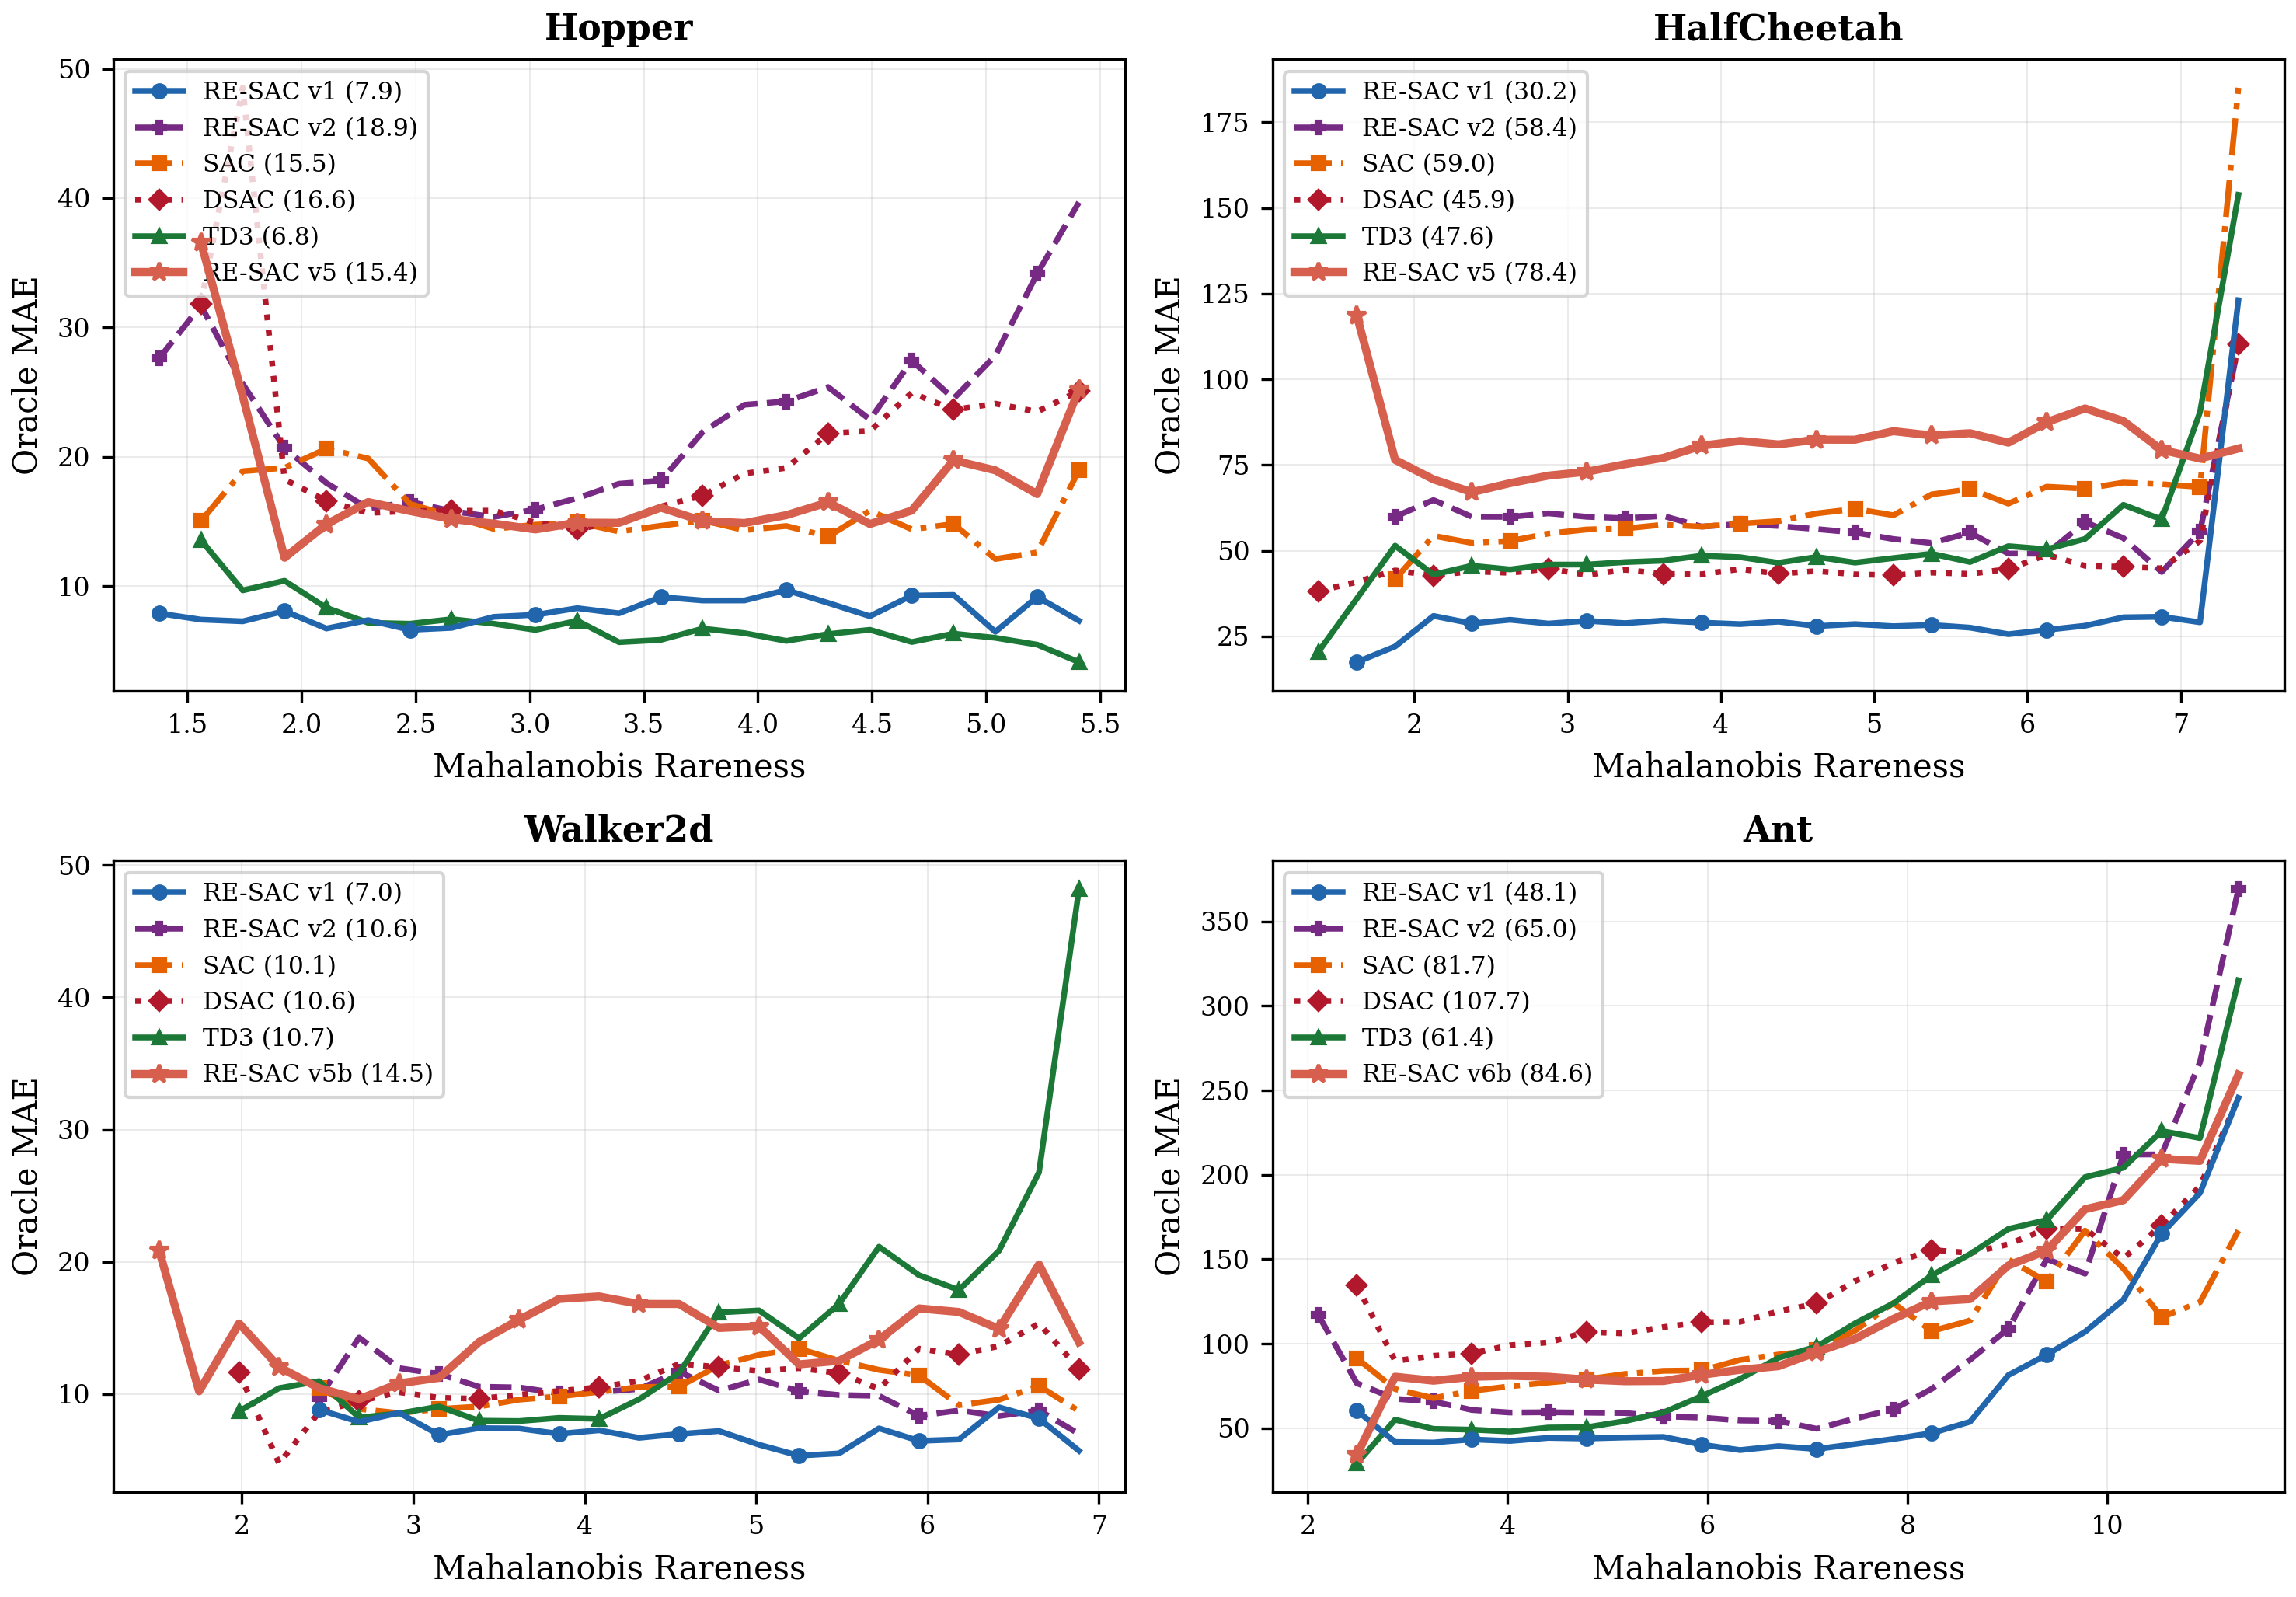
\includegraphics[width=\linewidth]{mujoco_oracle_q_error.png}
    \caption{Oracle Q-Error (MAE) binned by Mahalanobis rareness on four MuJoCo environments. Legend entries show overall Oracle MAE. RE-SAC v1 (solid blue) maintains the lowest estimation error in OOD regions; RE-SAC v5/v6b (red, starred) trades per-head accuracy for ensemble diversity that drives superior policy performance.}
    \label{fig:mujoco_oracle}
\end{figure}

\subsubsection{Training performance}
Fig.~\ref{fig:mujoco_curves} shows evaluation returns during training. RE-SAC v5 (thick red line, per-env best config) achieves the highest final return on all four environments: HalfCheetah 22711 (54\% above SAC), Walker2d 1008 (3.2$\times$ SAC, 2.2$\times$ DSAC), Hopper 660 (above SAC's 645), and Ant 27104 (v6b, surpassing DSAC's 25118). These gains stem from the independent target design preserving ensemble diversity: with meaningful Q-std, the adaptive $\beta_{lcb}$ schedule effectively balances exploration early (pessimistic $\beta{=}{-2}$) and exploitation later ($\beta \to -1$), while the EMA actor and policy anchor prevent the late-training instabilities observed in ablations without these mechanisms.

\begin{figure}[!htbp]
    \centering
    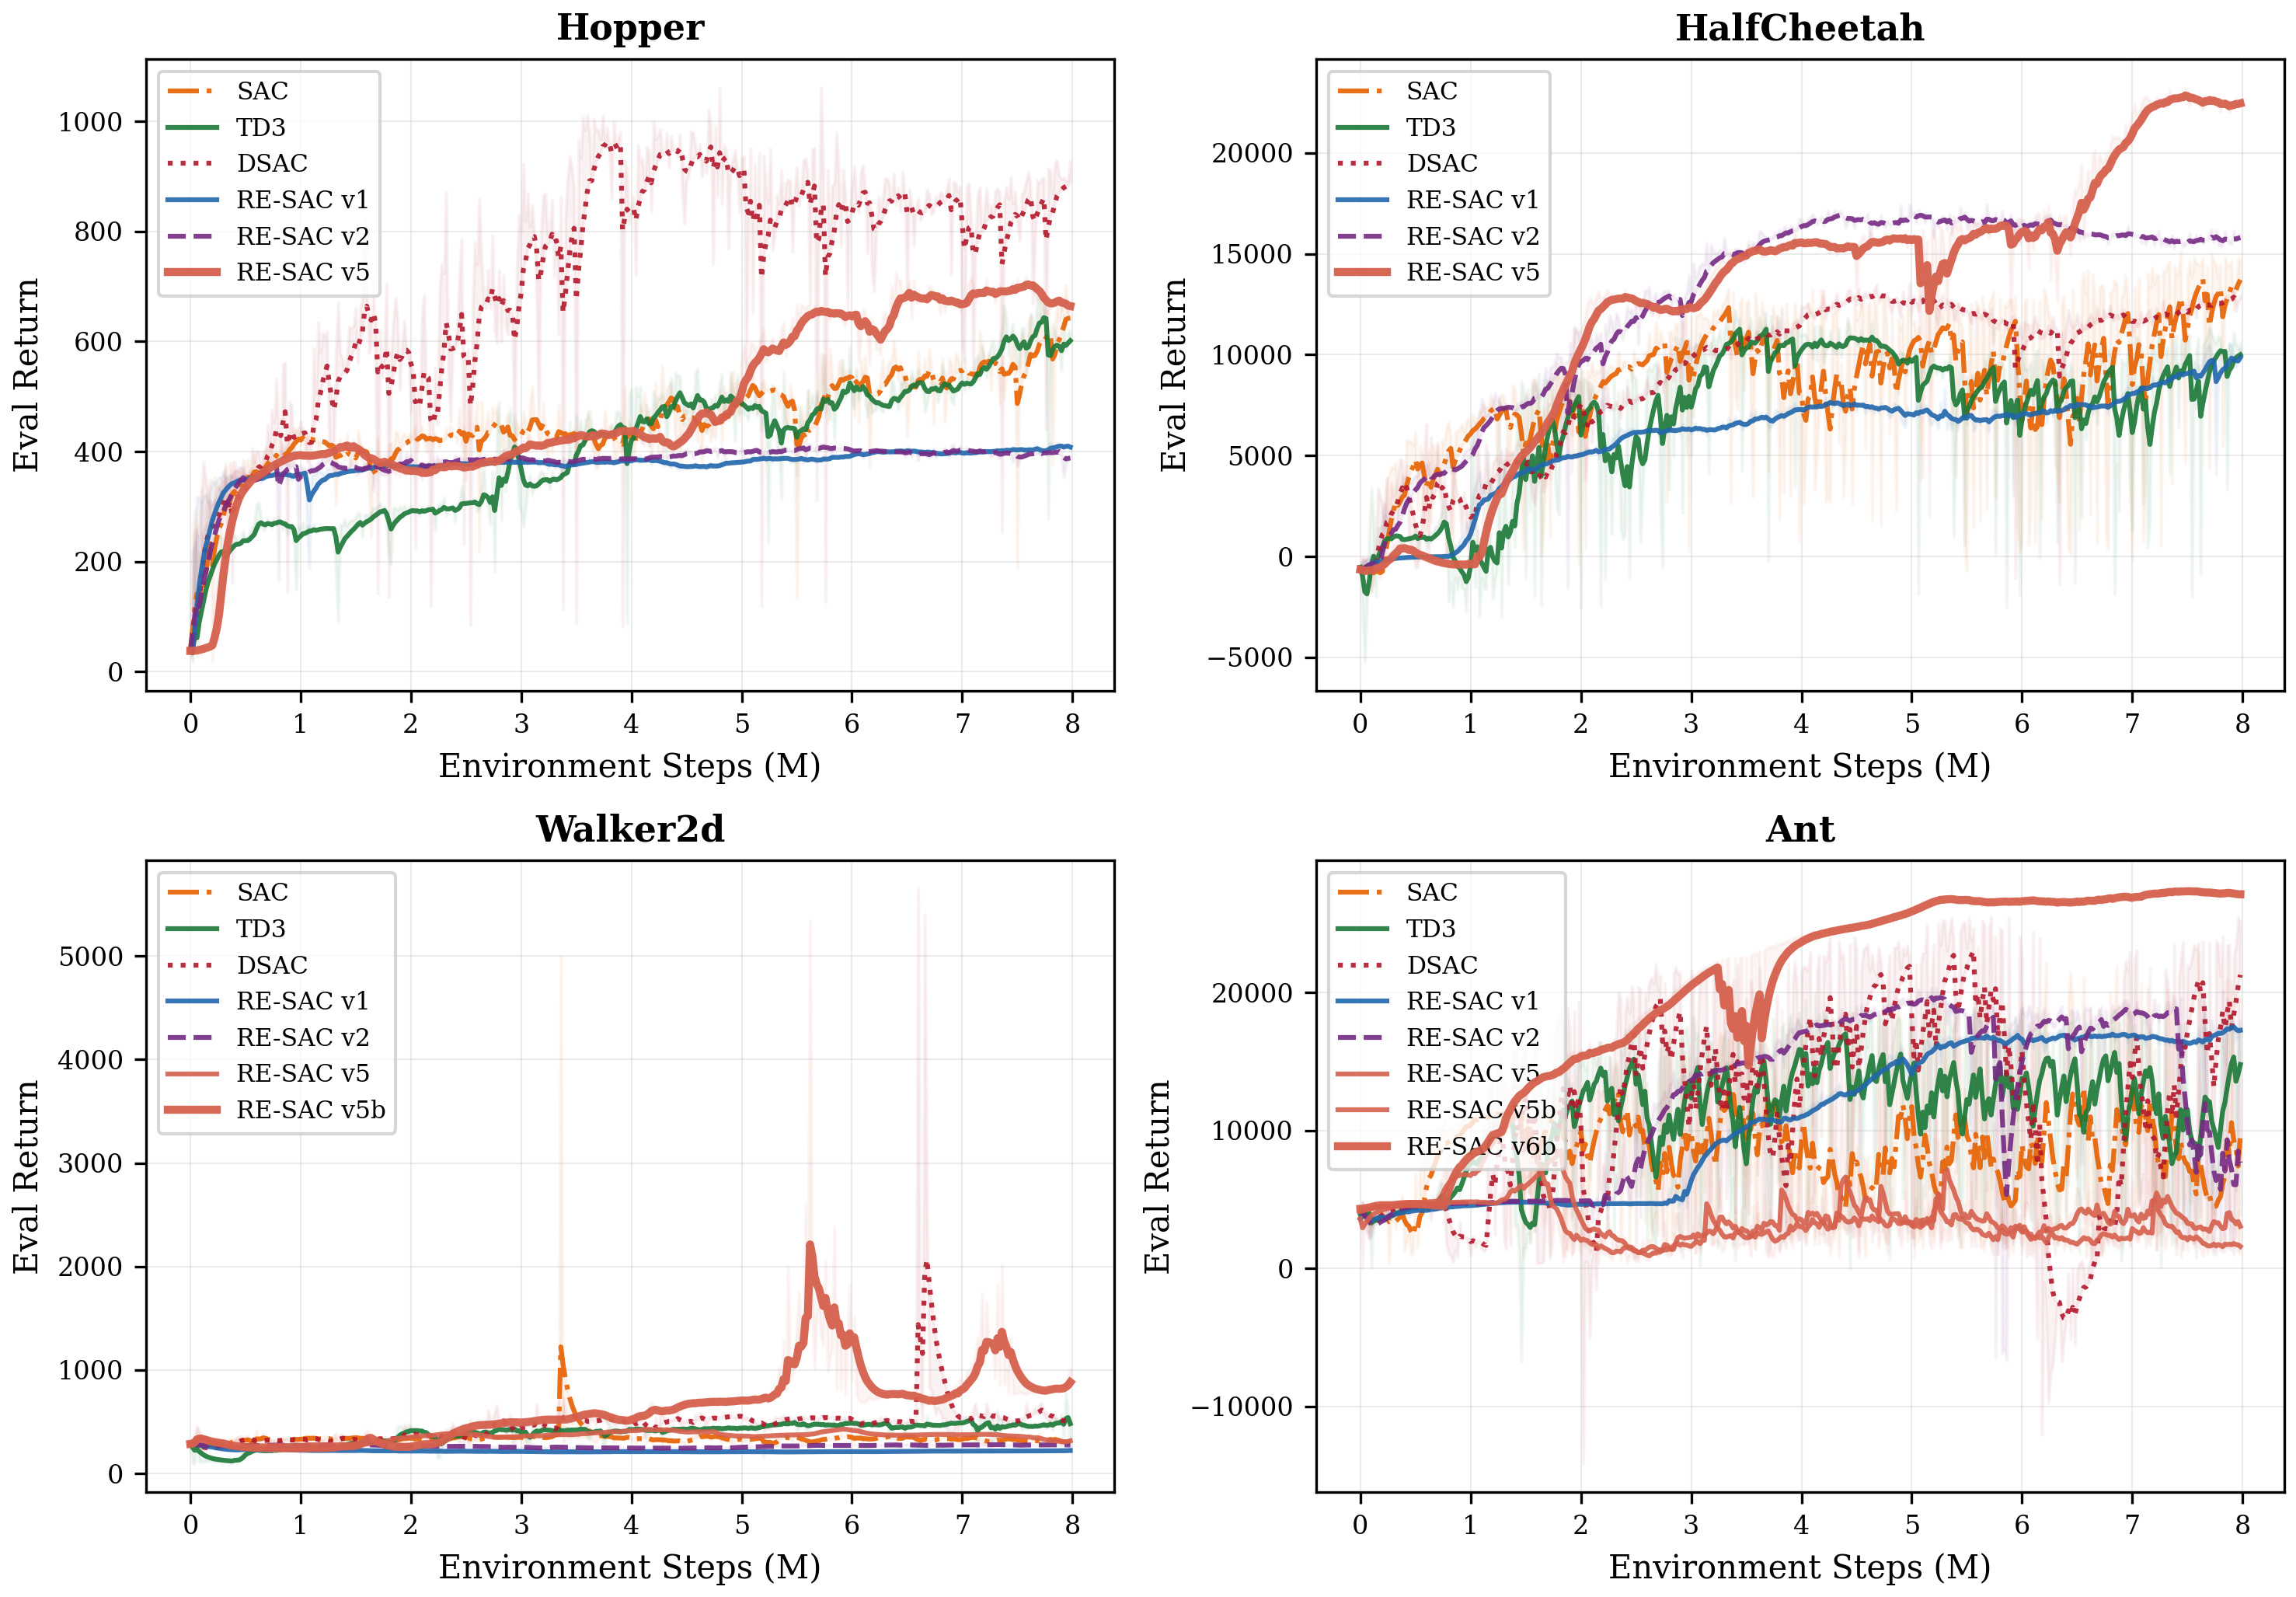
\includegraphics[width=\linewidth]{mujoco_training_curves.png}
    \caption{Evaluation returns on MuJoCo benchmarks (8M steps, seed 8). RE-SAC v5 (thick red) achieves the highest final return on all four environments by maintaining ensemble diversity through independent critic targets.}
    \label{fig:mujoco_curves}
\end{figure}

\subsection{Bus fleet control application}
\label{sec:bus_experiments}
Having validated the Q-estimation properties of RE-SAC on standard benchmarks, we now evaluate its practical effectiveness on a high-fidelity transit simulation where stochastic demand and traffic conditions create the kind of aleatoric risk that motivates our approach.

\subsubsection{Simulation environment}
We evaluate all algorithms on the bidirectional bus corridor simulation developed in our previous work~\cite{Zhang2025SingleAgentBus}. The environment models a realistic timetabled bus line with 22 stops (including two terminals) operating over a 13-hour service window (06:00--19:00). Buses are dispatched every 360 seconds from both terminals with a 180-second directional offset. Upon completing a trip, each vehicle becomes idle at its terminal and is available for reassignment according to the timetable, thereby modeling dynamic fleet sizing.

\textbf{Passenger demand} is specified by an hourly origin-destination (OD) matrix. For each pair of stations and each time period, passenger arrivals are sampled from a Poisson distribution with the corresponding time-varying rate. \textbf{Traffic conditions} are modeled as stochastic inter-stop travel speeds sampled from Gaussian distributions with hourly varying means and a fixed standard deviation of $\sigma = 1.5$~m/s, capturing realistic congestion fluctuations.

\textbf{MDP formulation.} The holding control problem is formulated as an event-driven MDP~\cite{Zhang2025SingleAgentBus}. Decisions are triggered after all passenger boarding/alighting activities have completed at each stop. The \textit{state} $s_t$ consists of categorical features (Bus~ID, Station~ID, Direction, Time~Period) and continuous features (forward headway $h_f$, backward headway $h_b$, current segment speed $v$). The \textit{action} $a_t \in [0, H_{max}]$ specifies the additional holding time at the current stop. The \textit{reward} follows the ridge-shaped function designed in~\cite{Zhang2025SingleAgentBus}, which simultaneously incentivizes headway regularity ($h_f \approx h_b \approx \tau$) and penalizes extreme deviations from the scheduled headway $\tau$.

\subsubsection{Network architecture and hyperparameters}
All algorithms are implemented in PyTorch. The $K$ critic networks are implemented as a single vectorized module (VectorizedCritic) for computational efficiency, each consisting of a 4-layer MLP with hidden dimensions $[64, 64, 64]$ and ReLU activations. The actor network is a separate 4-layer MLP with the same hidden dimension, outputting mean and log-standard-deviation for a squashed Gaussian policy. Following~\cite{Zhang2025SingleAgentBus}, categorical features (Bus~ID, Station~ID, Direction, Time~Period) are encoded via learnable embedding layers with dimension $d = \min(50, \lfloor N_i / 2 \rfloor)$, where $N_i$ is the number of unique categories. The embedded representations are concatenated with continuous state features (forward headway, backward headway, segment speed) to form the input vector.

Key hyperparameters are summarized as follows:
\begin{itemize}
    \item Ensemble size: $K \in \{2, 5, 10, 20, 40\}$ (default $K = 10$ unless otherwise specified);
    \item Learning rate: $1 \times 10^{-5}$ for critic, actor, and temperature (Adam optimizer);
    \item Batch size: 2048;
    \item Replay buffer size: $1 \times 10^6$ transitions;
    \item Discount factor: $\gamma = 0.99$;
    \item Target network smoothing coefficient: $\tau = 0.01$;
    \item Aleatoric regularization coefficient: $\lambda_{ale} = 0.01$ ($\ell_1$ weight penalty in critic target and loss; cf.\ Eq.~8);
    \item Actor LCB weight: $\beta_{lcb} = -2$ (applied as $\bar{Q} + \beta_{lcb} \cdot \sigma_{ens}$ in the actor objective; cf.\ Eq.~14);
    \item OOD penalty coefficient: $\beta_{ood} = 0.01$ (penalizes ensemble standard deviation in critic loss; cf.\ Eq.~12);
    \item Entropy temperature $\alpha$: automatically tuned via dual gradient descent with target entropy $\mathcal{H}_{target} = -\dim(\mathcal{A})$, capped at $\alpha_{\max} = 0.6$;
    \item Gradient clipping: max norm $= 1.0$;
    \item Critic-to-actor update ratio: $2:1$.
\end{itemize}
All baseline algorithms (SAC, DSAC, BAC) share the same network architecture, learning rate, and buffer configuration for fair comparison. Each experiment is trained for 500 episodes with training updates triggered every 5 environment steps, and evaluation metrics are averaged over 10 independent rollouts.

\subsubsection{Baselines and ablations}
To comprehensively evaluate our proposed method, we compare RE-SAC against state-of-the-art baselines and perform ablation studies to isolate the impact of our risk disentanglement.
\begin{itemize}
    \item \textbf{Vanilla SAC}~\cite{Haarnoja2018SAC}: The standard Soft Actor-Critic algorithm without explicit robust regularization or ensemble pessimism.
    \item \textbf{DSAC}~\cite{Ma2025DSAC}: Distributional Soft Actor-Critic, a risk-sensitive variant that learns the continuous return distribution to handle environmental stochasticity.
    \item \textbf{BAC}~\cite{Ji2024SeizingSerendipity}: BEE Actor-Critic~\cite{Ji2024SeizingSerendipity}, an off-policy actor-critic that exploits past successful experiences via the Blended Exploitation and Exploration (BEE) operator to avoid catastrophic value underestimation. We abbreviate it BAC (BEE Actor-Critic) throughout for brevity.
    \item \textbf{Epistemic only (ablation)}: A variant of RE-SAC that only applies the ensemble variance penalty $\Gamma_{epi}$, omitting the aleatoric weight regularization.
    \item \textbf{Aleatoric only (ablation)}: A variant that only applies the IPM-based weight regularization $\Gamma_{ale}$, omitting the ensemble.
\end{itemize}
For RE-SAC, we also evaluate the effect of the ensemble size $K \in \{2, 5, 10, 20, 40\}$.

\subsubsection{Overall performance and learning stability}
Fig.~\ref{fig:all_experiments} displays the smoothed cumulative rewards over training. Vanilla SAC and the Aleatoric-Only ablation suffer from suboptimal convergence, plateauing around a reward of $-0.55 \times 10^6$. The purely distributional baseline, DSAC-v1, performs slightly better but still falls short of the proposed method. Notably, the Epistemic-Only variant experiences a complete catastrophic collapse mid-training, dropping to $-1.2 \times 10^6$. This confirms our hypothesis: relying solely on ensemble variance in a highly stochastic environment misidentifies inherent noise as missing data, leading to runaway pessimism and policy degradation.

By successfully disentangling the uncertainties, RE-SAC (particularly with moderate ensemble sizes $K=5, 10, 20$) achieves the highest and most stable final reward (around $-0.4 \times 10^6$). Excessively large ensembles ($K=40$) show a slight performance degradation: with 40 parallel critics, the accumulated variance penalty $\lambda_{epi}\Gamma_{epi}$ becomes more sensitive to transient disagreements during early training, inducing a conservative bias that persists and slightly suppresses the final reward. This is consistent with the known over-pessimism of large ensembles in online settings~\cite{An2021UncertaintyEnsemble}. 
The BAC baseline, designed to avoid underestimation by exploiting past successes, performs relatively well but exhibits higher variance during training compared to RE-SAC, settling at a slightly lower final reward than the best RE-SAC variants. This suggests that while maintaining optimistic estimates of past serendipitous events helps avoid complete policy collapse in stochastic environments, explicitly disentangling and regularizing against aleatoric and epistemic risks provides a more stable and robust policy improvement path.

\begin{figure}[!htbp]
    \centering
    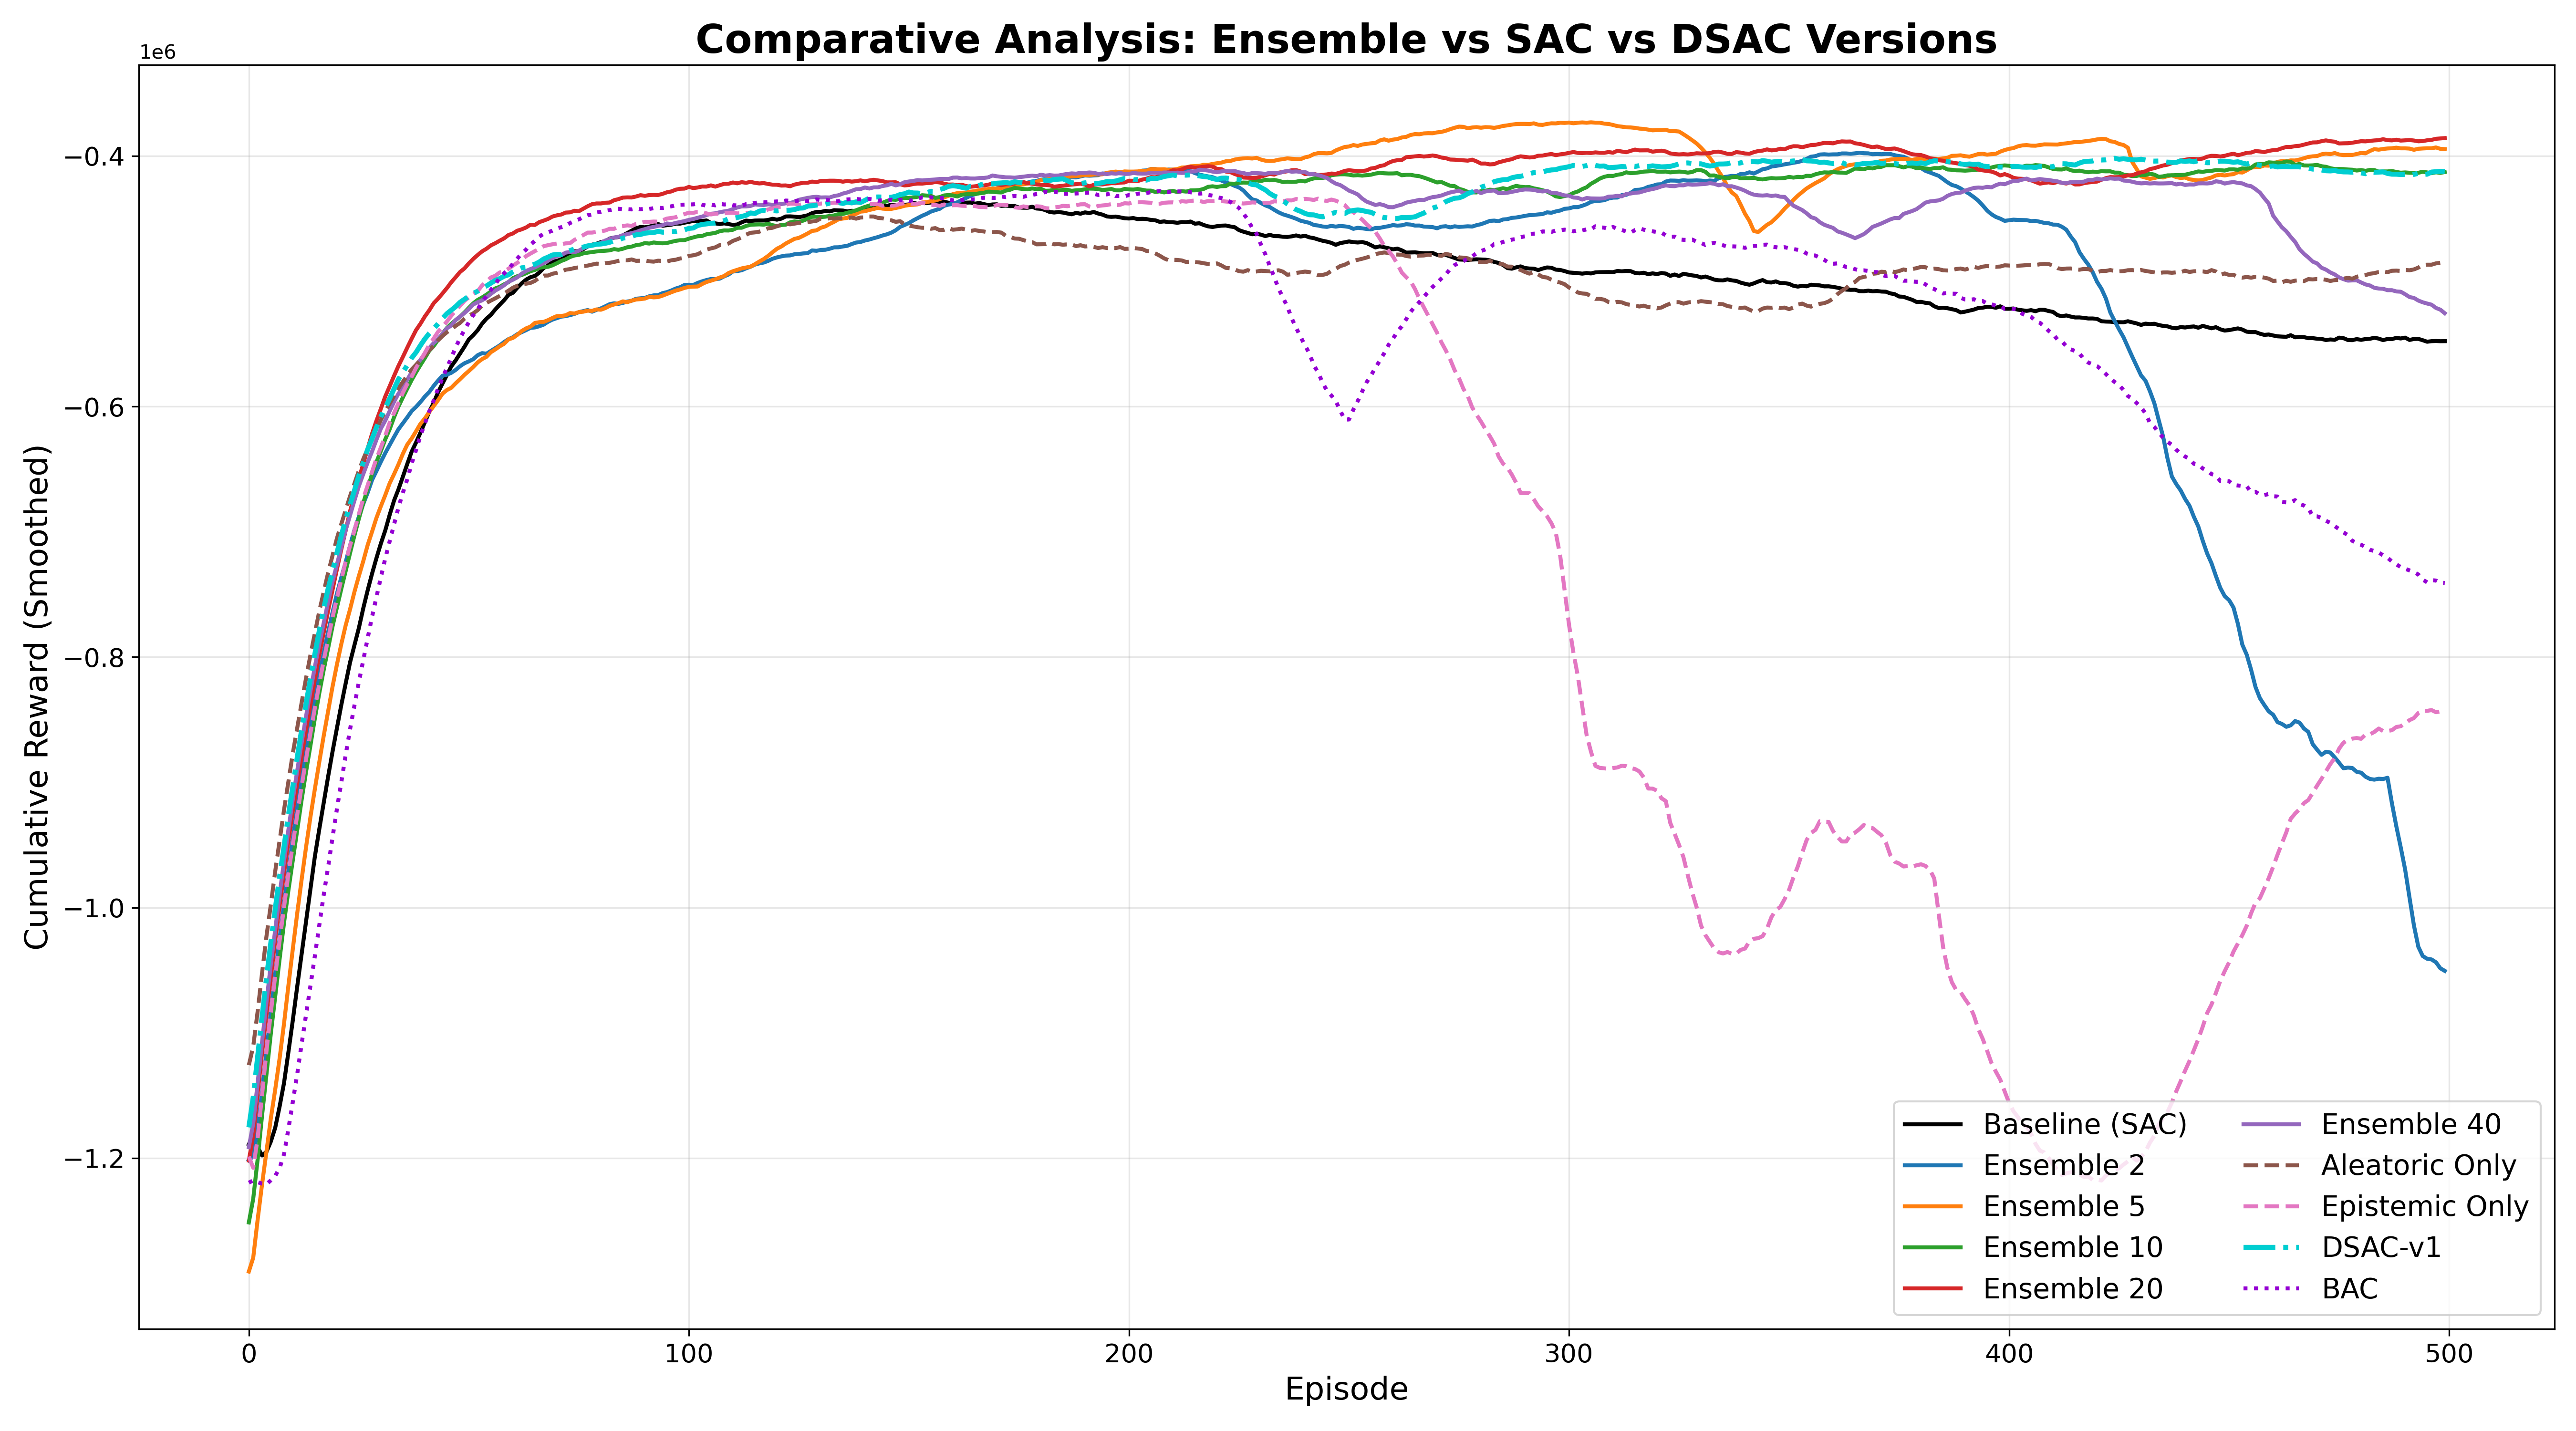
\includegraphics[width=\linewidth]{all_experiments_comparison_v2.png}
    \caption{Learning curves of cumulative reward for RE-SAC variants, SAC, DSAC-v1, BAC, and ablations.}
    \label{fig:all_experiments}
\end{figure}

\subsubsection{Q-value estimation stability}
The catastrophic drop in the Epistemic-Only policy is directly correlated with extreme value underestimation. As shown in Fig.~\ref{fig:all_q_values}, the estimated Q-values for the Epistemic-Only ablation plummet deep into negative values (passing $-3000$) with a massive $2\sigma$ variance band, corroborating the ``underestimation trap''. In contrast, RE-SAC variants and baseline SAC maintain relatively stable Q-value ranges. The disentangled penalties in RE-SAC prevent the variance penalty from overwhelming the nominal expected return.

\begin{figure}[!htbp]
    \centering
    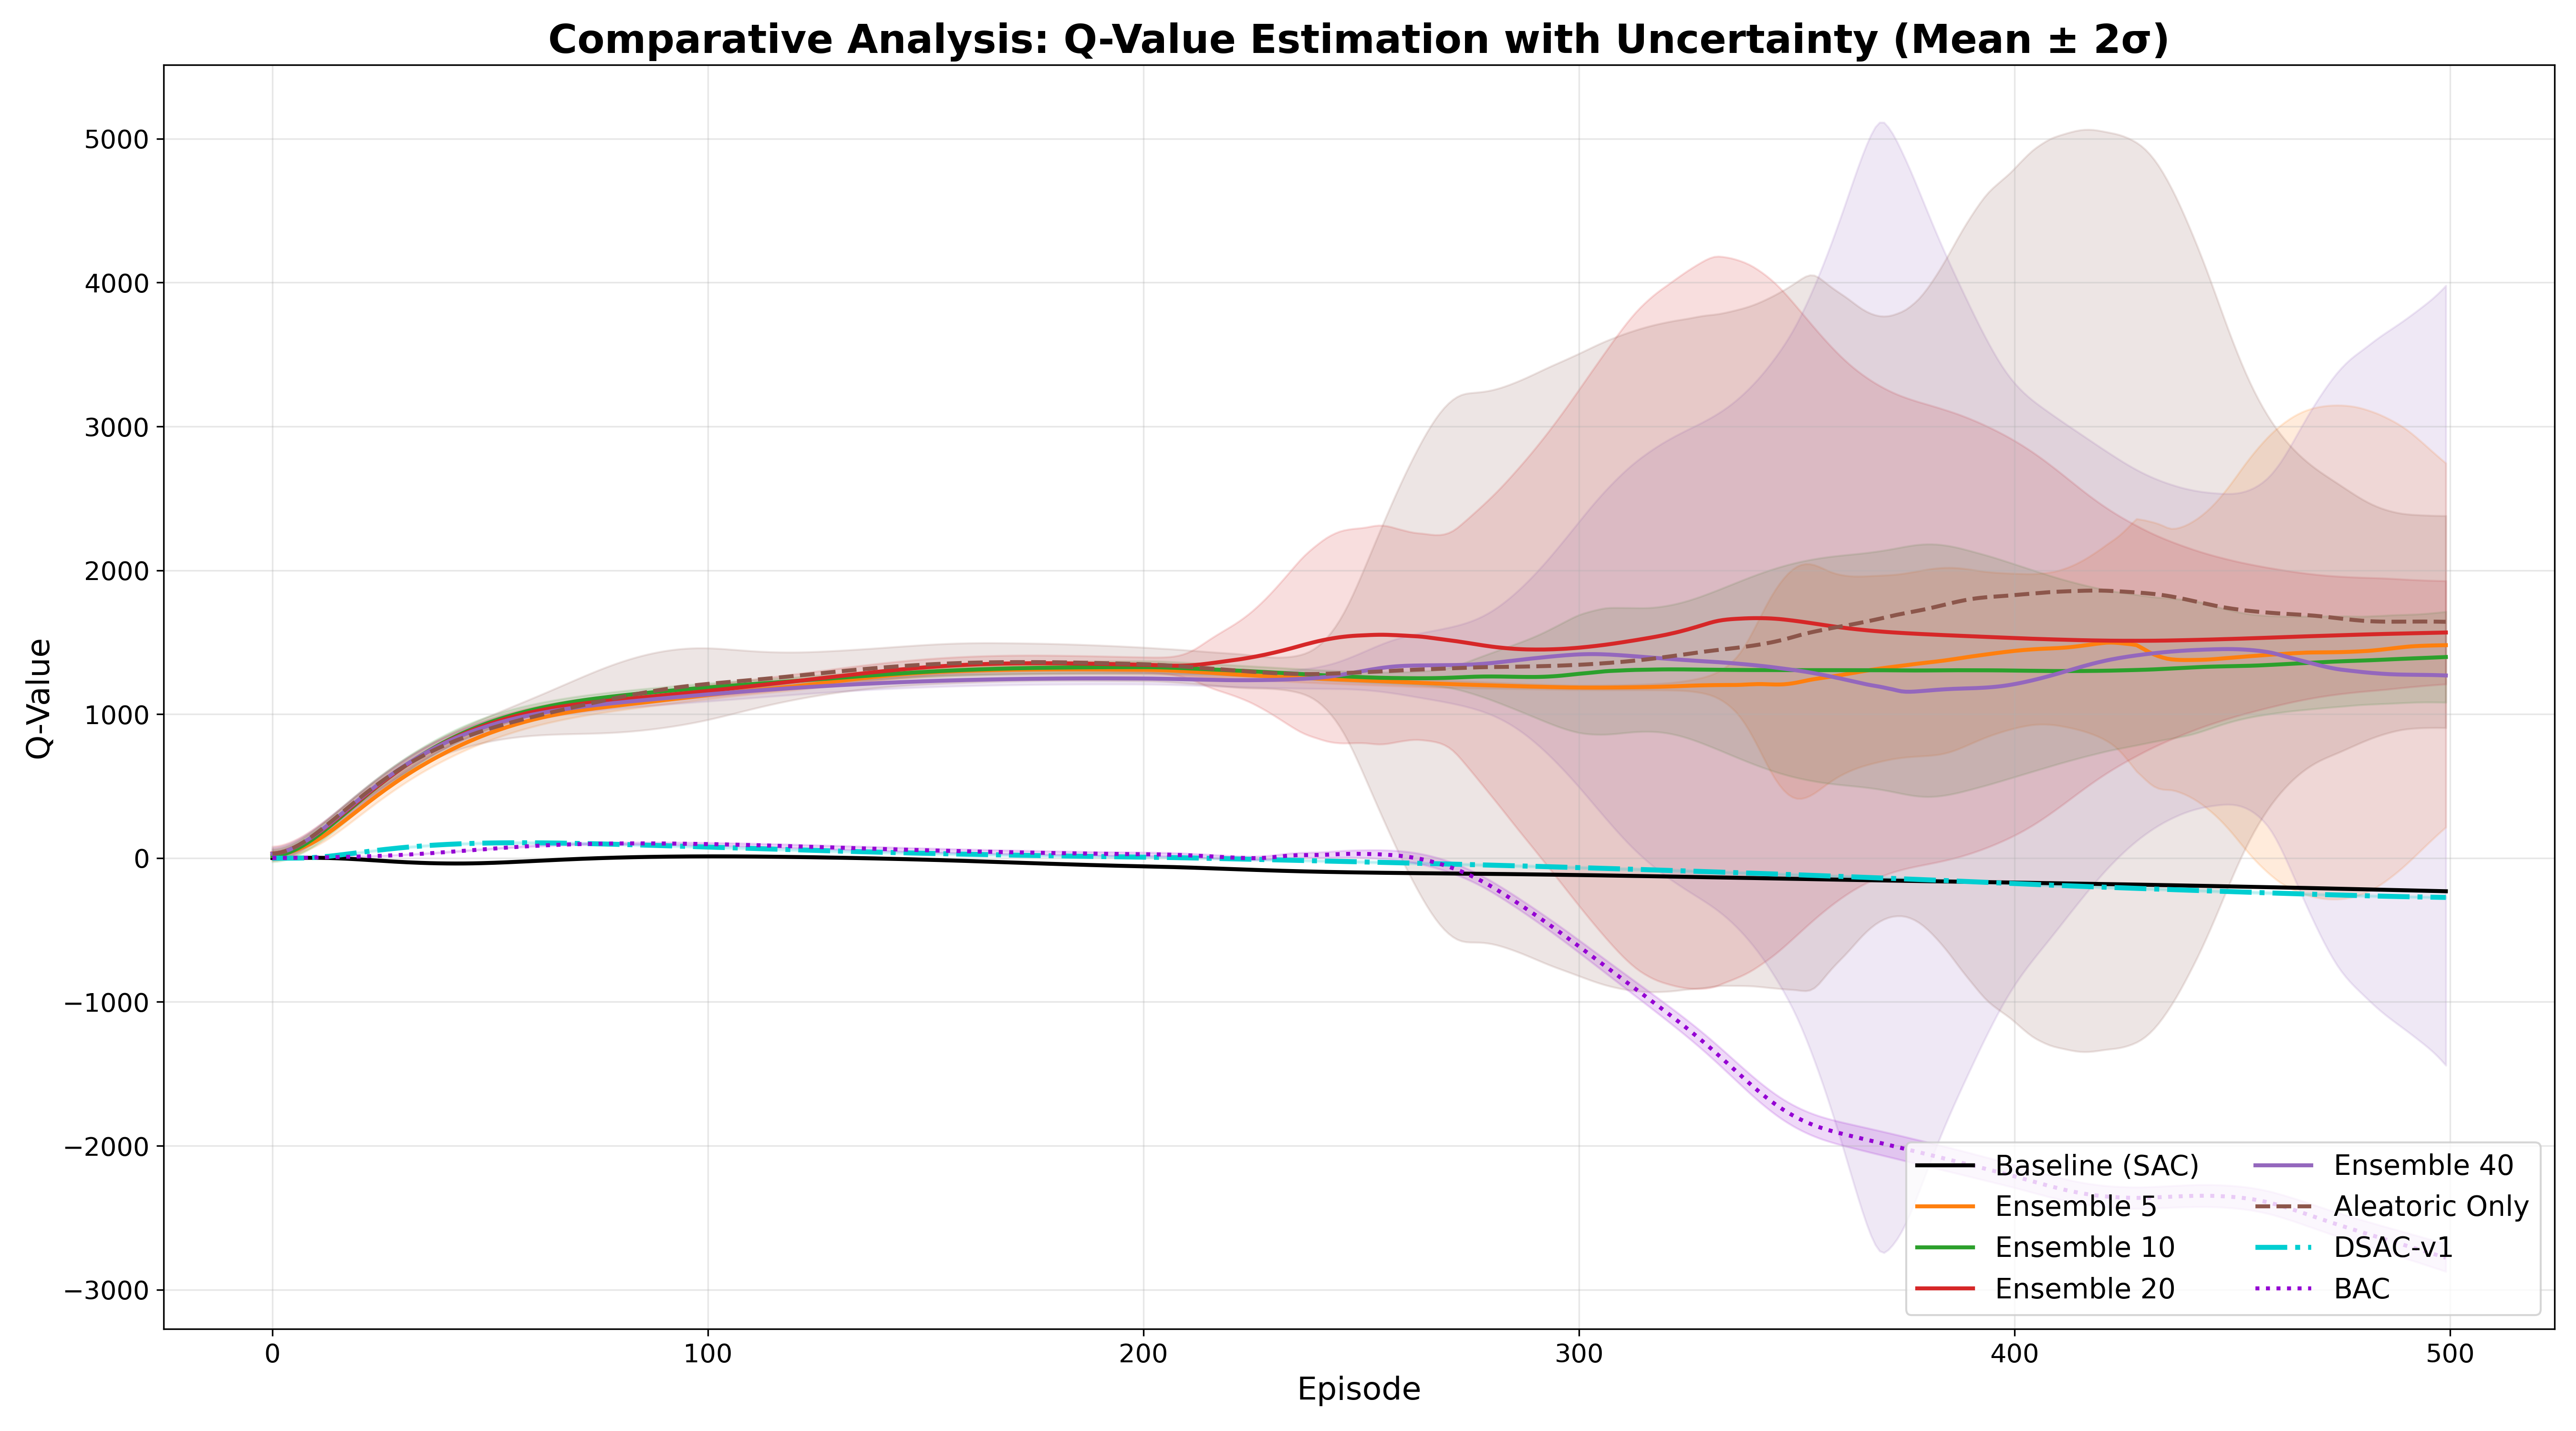
\includegraphics[width=\linewidth]{all_q_values_comparison_v2.png}
    \caption{Comparative analysis of estimated Q-Values (Mean $\pm$ $2\sigma$) over training.}
    \label{fig:all_q_values}
\end{figure}

\subsubsection{Robustness in rare states (Mahalanobis rareness)}
While the preceding Q-value analysis tracks estimation stability \emph{over training episodes}, a robust optimization perspective demands a complementary view: \emph{at the same level of state rarity, does the algorithm produce smaller estimation errors than baselines?} This distinction is essential because robust policies are valued not for their average-case accuracy, but for their ability to maintain bounded estimation errors in the worst-case regions of the state space.

To formalize this, we define \textbf{Mahalanobis rareness}. The key design choices are as follows. First, we condition on each \emph{spatial-directional group} (Station~ID $\times$ Direction), because different stops exhibit fundamentally different nominal headway distributions---for example, departure headways at terminals are tightly constrained by the timetable, whereas mid-route headways are subject to cumulative disturbances. A single global distribution would conflate structurally different operating regimes. For each group, we fit a 2D Gaussian to the observed continuous features (Forward Headway, Backward Headway), estimating the empirical mean $\mu$ and covariance $\Sigma$. Second, we use the \emph{Mahalanobis distance} rather than a simple Euclidean norm because the two headway features have different scales and are correlated (e.g., a very large forward headway typically co-occurs with a small backward headway in a bunching event). Euclidean distance is sensitive to these scale differences and ignores feature correlations, whereas the Mahalanobis distance $\sqrt{(x-\mu)^T\Sigma^{-1}(x-\mu)}$ naturally normalizes by the feature covariance, so that equally likely headway combinations receive equal rareness scores regardless of their direction in feature space. Intuitively, a state with high Mahalanobis rareness is one whose headway configuration the agent has rarely encountered at that stop during training---precisely the kind of state where epistemic risk is highest.

Fig.~\ref{fig:mahalanobis} bins the Mean Absolute Error (MAE) between each algorithm's Q-value estimates and the ground-truth Monte Carlo return $Q_{MC}(s,a)$ by Mahalanobis rareness. Here, $Q_{MC}$ is computed offline from the recorded evaluation trajectories as the discounted cumulative reward from each decision point onward: $Q_{MC}(s_t, a_t) = \sum_{k=0}^{T-t} \gamma^k r_{t+k}$, providing a model-free ground truth independent of any learned value function.

Since different algorithms learn Q-values at different absolute scales, direct comparison of raw prediction errors would be misleading. We therefore apply a per-algorithm z-score alignment that rescales each algorithm's predictions to match the mean and standard deviation of $Q_{MC}$ before computing the error. Additionally, for ensemble-based algorithms, we report the \textbf{Oracle MAE}: for each state, we select the ensemble head whose aligned prediction is closest to $Q_{MC}$, and compute the MAE over these best-head predictions. This oracle serves as a favorable upper bound on the ensemble's representational capacity---it measures how well the ensemble \textit{could} estimate the true return if paired with an ideal head-selection mechanism.

As states become increasingly rare (moving left to right on the x-axis), the estimation errors for Vanilla SAC and DSAC-v1 escalate significantly, confirming that their value networks extrapolate unreliably outside the training distribution. In contrast, RE-SAC (Ensemble) consistently demonstrates the lowest Oracle MAE across all rareness bins (overall average of 1647, compared to SAC's 4343 and DSAC's 5945). The tight error bands around the RE-SAC predictions confirm that the disentangled regularization structurally bounds the value network, preventing wild extrapolations in OOD regions and yielding superior worst-case guarantees.
\vspace{-2pt}
\begin{figure}[!htbp]
    \centering
    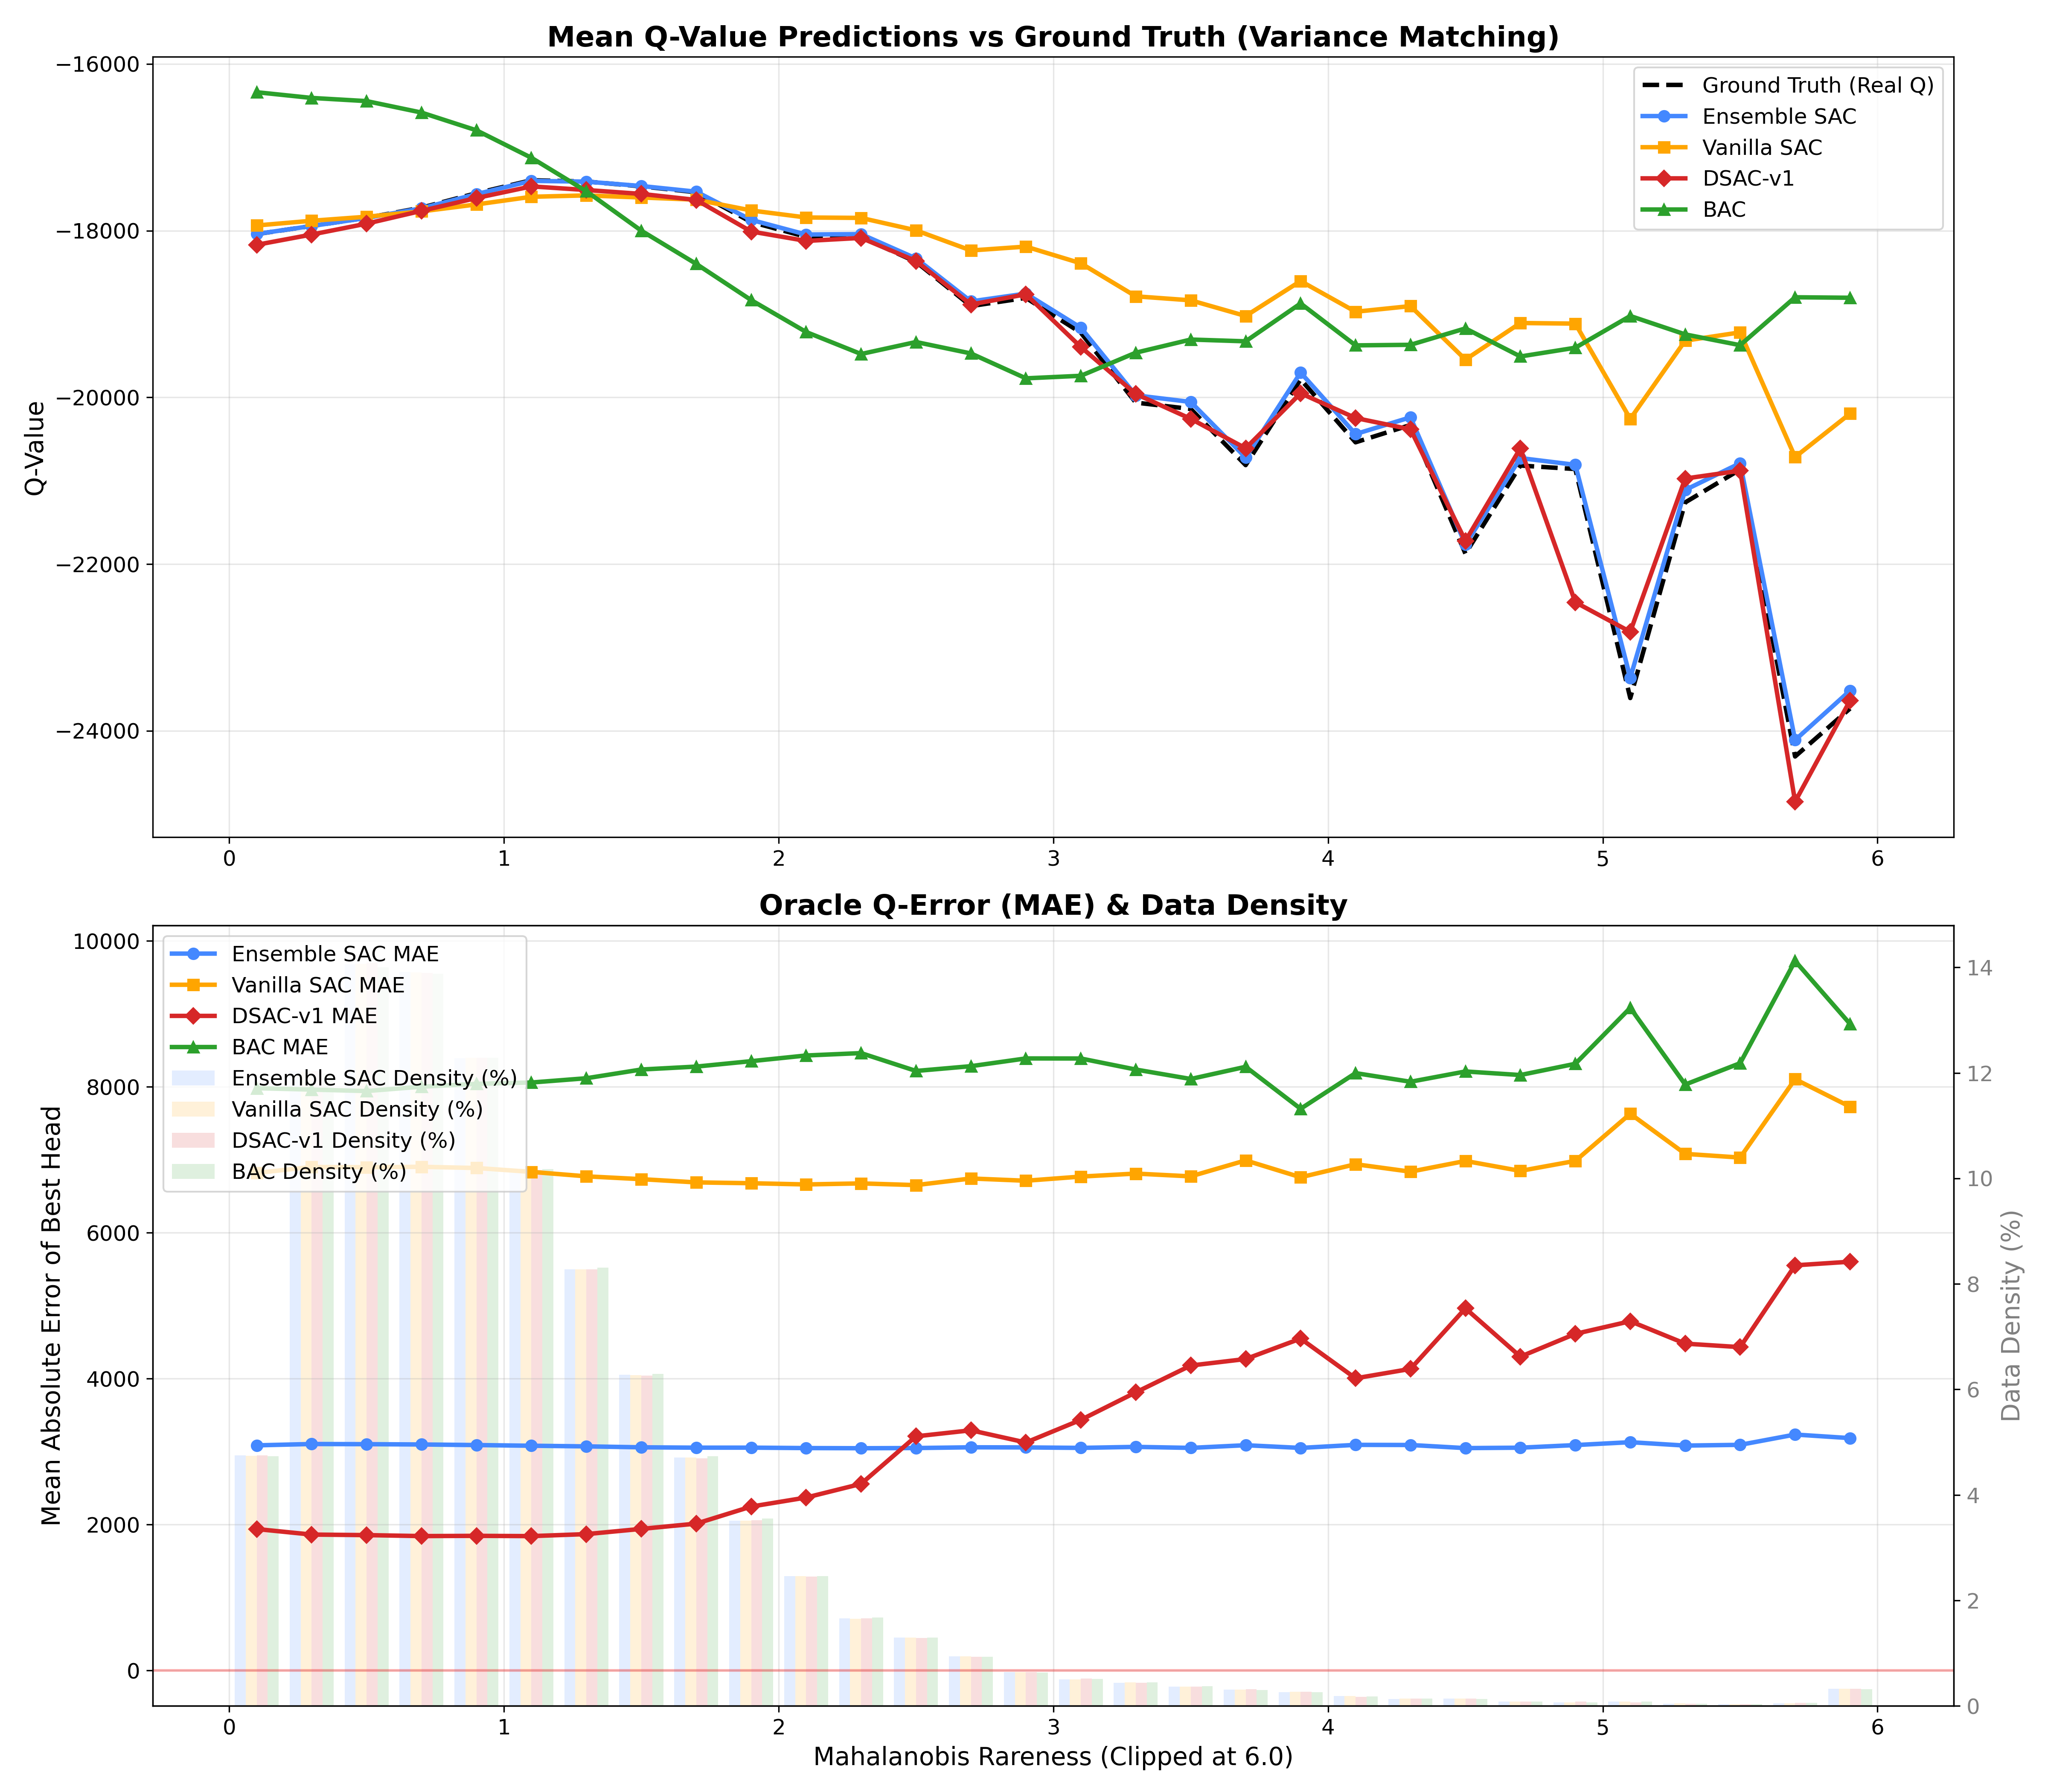
\includegraphics[width=\linewidth]{comparison_mahalanobis_rareness_restyled.png}
    \vspace{-6pt}
    \caption{Oracle Q-Error (MAE) banded by Mahalanobis Rareness. RE-SAC maintains accurate estimates even in highly rare/OOD states.}
    \label{fig:mahalanobis}
\end{figure}

\FloatBarrier
\section{Conclusion}
This paper presents the RE-SAC framework, a robust reinforcement learning approach that explicitly disentangles aleatoric and epistemic uncertainties. Grounded in the theoretical correspondence between risk-sensitivity and robustness established by Osogami~\cite{Osogami2012Robustness}, our method employs two complementary mechanisms: IPM-based weight regularization to enforce Lipschitz continuity of the value function against inherent environmental stochasticity, and a diversified $Q$-ensemble to penalize overconfident estimates in data-sparse regions of the state-action space.

Our theoretical analysis identifies a sharp structural boundary for contraction in multi-penalty Bellman operators: the frozen-parameter design (target networks for epistemic variance, held-fixed critic weights for aleatoric penalty) is both sufficient for $\gamma$-contraction and \emph{necessary}---Q-dependent penalties provably break it.  Both results are machine-verified in Lean~4 with no \texttt{sorry}, and a verifiable feasibility condition on the penalty coefficients guarantees policy non-degeneration (Appendix~\ref{app:nondegen}).  This structural insight---that the standard deep RL architecture of frozen target networks is not merely a stabilisation heuristic but a \emph{required} condition for operator contractiveness---may inform the design of future multi-penalty RL algorithms.

Empirically, on standard MuJoCo benchmarks, RE-SAC achieves the lowest Oracle Q-estimation error on 3 of 4 environments, reducing MAE by up to 55\% relative to DSAC and 41\% relative to SAC on the high-dimensional Ant task. On a realistic bidirectional bus simulation, RE-SAC achieves the highest and most stable cumulative reward among all baselines, including vanilla SAC, DSAC, and BAC. The ablation studies reveal that relying solely on ensemble variance (Epistemic-Only) leads to catastrophic value collapse in high-variance transit environments, while using only weight regularization (Aleatoric-Only) fails to detect out-of-distribution states. The Mahalanobis rareness analysis further confirms that RE-SAC maintains accurate $Q$-value estimates even under highly rare traffic states, exhibiting superior worst-case robustness.

In future work, we plan to extend this framework to multi-line transit networks with transfer coordination, investigate adaptive scheduling of the uncertainty coefficients $\lambda_{ale}$ and $\lambda_{epi}$ during training, and explore the integration of distributional RL methods with our disentangled robustness framework to further improve tail-risk management in urban transit systems.

\section*{Acknowledgments}
This work was supported by the National Natural Science Foundation of China (Grant No. 72371251), the Natural Science Foundation for Distinguished Young Scholars of Hunan Province (Grant No. 2024JJ2080), and the Key Research and Development Program of Hunan Province of China (Grant No. 2024JK2007).

\bibliographystyle{IEEEtran}
\documentclass[10pt]{article}
\usepackage[utf8]{inputenc}
\usepackage[T1]{fontenc}
\usepackage[margin=1in, left=1.25in, right=1.25in, top=1in, bottom=1in]{geometry}
\usepackage{algorithm}
\usepackage{algorithmic}
\usepackage[linktoc=all, bookmarksdepth=3, pdfstartview=FitH]{hyperref}
\hypersetup{colorlinks=true, linkcolor=blue, filecolor=magenta, urlcolor=cyan}
\urlstyle{same}
\usepackage{amsmath}
\usepackage{amsfonts}
\usepackage{amssymb}
\usepackage[version=4]{mhchem}
\usepackage{stmaryrd}
\usepackage{bbold}
\usepackage{graphicx}
\usepackage[export]{adjustbox}
\usepackage[dvipsnames]{xcolor}
\usepackage{float}
\usepackage{placeins}
\usepackage{caption}
\captionsetup[figure]{name=Fig.}
\usepackage{booktabs}
\usepackage{multirow}
% ==== Revision color macro (keep for marked version) ====
\usepackage[normalem]{ulem} % for \sout
\usepackage{amsthm}
\usepackage{enumitem}
\newtheorem{theorem}{Theorem}[section]
\newtheorem{lemma}[theorem]{Lemma}
\newtheorem{definition}[theorem]{Definition}
\newtheorem{corollary}[theorem]{Corollary}
\newtheorem{proposition}[theorem]{Proposition}
\newtheorem{remark}[theorem]{Remark}
% \newcommand{\revise}[1]{{\color{blue}#1}}
% \newcommand{\del}[1]{\color{red}{\sout{#1}}}             % deletions (red strikeout)
\newcommand{\revise}[1]{#1}
\newcommand{\del}[1]{}

% ==== Algorithm package ====
% Option A: algorithm2e
% \usepackage[ruled,vlined,linesnumbered]{algorithm2e}
% Or Option B: algpseudocode


\graphicspath{ {./} }

\title{RE-SAC: Disentangling aleatoric and epistemic risks in bus fleet control: A stable and robust ensemble DRL approach\footnote{Code available at \url{https://github.com/erzhu419/RE-SAC}}}

\author{
  Yifan Zhang\thanks{Central South University, \href{mailto:erzhu419@gmail.com}{erzhu419@gmail.com}, \href{mailto:204201048@csu.edu.cn}{204201048@csu.edu.cn}} \and
  Liang Zheng\thanks{Central South University, \href{mailto:zhengliang@csu.edu.cn}{zhengliang@csu.edu.cn}}
}
\date{}


%New command to display footnote whose markers will always be hidden
\let\svthefootnote\thefootnote
\newcommand\blfootnotetext[1]{%
  \let\thefootnote\relax\footnote{#1}%
  \addtocounter{footnote}{-1}%
  \let\thefootnote\svthefootnote%
}

%Overriding the \footnotetext command to hide the marker if its value is `0`
\let\svfootnotetext\footnotetext
\renewcommand\footnotetext[2][?]{%
  \if\relax#1\relax%
    \ifnum\value{footnote}=0\blfootnotetext{#2}\else\svfootnotetext{#2}\fi%
  \else%
    \if?#1\ifnum\value{footnote}=0\blfootnotetext{#2}\else\svfootnotetext{#2}\fi%
    \else\svfootnotetext[#1]{#2}\fi%
  \fi
}

\begin{document}
\maketitle


\begin{abstract}
Bus holding control remains a persistent challenge in urban transit systems due to the inherent stochasticity of traffic conditions and passenger demand. While deep reinforcement learning (DRL) has shown promise for dynamic holding decisions, standard actor-critic algorithms frequently suffer from $Q$-value instability in highly volatile environments. A key yet underexplored source of this instability is the conflation of two structurally distinct uncertainties: \textit{aleatoric} uncertainty, arising from irreducible environmental noise, and \textit{epistemic} uncertainty, arising from data insufficiency in the replay buffer. Treating these as a single risk leads to pathological underestimation in well-explored but noisy states, ultimately causing catastrophic value collapse.

In this paper, we propose a robust ensemble soft actor-critic (RE-SAC) framework that explicitly disentangles and addresses both sources of uncertainty. Our approach applies Integral Probability Metric (IPM)-based weight regularization to the critic network to hedge against aleatoric risk, providing a smooth analytical lower bound for the robust Bellman operator without requiring expensive inner-loop state perturbations. To address epistemic risk, a diversified $Q$-ensemble penalizes overconfident value estimates in sparsely covered regions of the state-action space. This dual mechanism prevents the ensemble variance from misidentifying inherent noise as a data gap, a failure mode that causes complete policy collapse in our ablation study.

Empirically, experiments in a realistic bidirectional bus corridor simulation demonstrate that RE-SAC achieves the highest and most stable cumulative reward (approximately $-0.4 \times 10^6$) among all baselines, compared to $-0.55 \times 10^6$ for vanilla SAC and $-1.2 \times 10^6$ for the epistemic-only ablation. The Mahalanobis rareness analysis further confirms that RE-SAC reduces \emph{Oracle} Q-value estimation error by up to $62\%$ in rare out-of-distribution states relative to SAC (average Oracle MAE of 1647 vs.\ 4343), demonstrating superior worst-case robustness under high traffic variability.
Our theoretical analysis further reveals that the frozen-parameter design (target networks, held-fixed critic weights) is not merely a practical stabilisation heuristic but a \emph{structurally necessary condition} for Bellman operator contractiveness under multi-penalty regularisation---an insight with implications beyond transit control.
\end{abstract}


\noindent\textbf{Keywords:} bus bunching; robust reinforcement learning; ensemble; uncertainty decomposition; bus holding control.


\section{Introduction}

Bus bunching---the phenomenon where multiple buses on the same route cluster together---remains a well-known challenge in urban transit systems. This instability is driven by a positive feedback loop: a slight delay at a stop increases passenger accumulation, which extends dwell time, further slowing the leading bus while the trailing bus speeds up due to reduced demand~\cite{Daganzo2009Headway, Xuan2011Dynamic}. To break this cycle, various holding control strategies have been developed, transitioning from classical schedule-based optimization to deep reinforcement learning (DRL) paradigms~\cite{Wang2020DynamicHolding}.
However, despite the promising performance of DRL in controlled simulations, these models often exhibit fragile behavior when deployed in realistic, high-variance transit environments.

A critical, yet frequently overlooked bottleneck in applying Actor-Critic methods to transit control is what we term ``$Q$-value poisoning.'' In public transportation, stochasticity is not a transient disturbance but a deeply ingrained feature; fluctuations in passenger arrival rates and road traffic speeds are often irreducible. In such highly volatile environments, standard off-policy algorithms like Soft Actor-Critic (SAC) frequently suffer from pathological value estimation degradation. As training progresses, the $Q$-function may become ``poisoned'' by environmental noise, leading to severe underestimation of successful past interventions or wild oscillations in unvisited state-action regions. This phenomenon, consistent with the ``value collapse'' identified by recent studies~\cite{Ji2024SeizingSerendipity}, effectively paralyzes the agent's policy, causing it to fall into an under-exploitation trap where it fails to maintain regularity despite having encountered optimal trajectories in its experience buffer.

\begin{definition}[$Q$-value Poisoning]
    \label{def:poisoning}
    Let $Q^*$ be the optimal $Q$-function and $Q_t$ be the learned $Q$-function after $t$ gradient steps.
    Let $\sigma^2(s,a) := \mathrm{Var}_{P}[V_t(s') \mid s,a]$ denote the local aleatoric variance at $(s,a)$.
    We say the learning process suffers from \emph{$Q$-value poisoning} if there exist
    a threshold $\sigma^2_0 > 0$ and a non-vanishing set of state-action pairs
    $\mathcal{P}_t \subseteq \mathcal{S}\times\mathcal{A}$ such that:
    \begin{enumerate}[label=(\roman*)]
        \item \textbf{Selective underestimation in high-variance regions:}
        $Q_t(s,a) < Q^*(s,a)$ for all $(s,a)\in\mathcal{P}_t$ with
        $\sigma^2(s,a) \ge \sigma^2_0$; and
        \item \textbf{Accurate estimation in low-variance regions:}
        $|Q_t(s,a) - Q^*(s,a)| \le \epsilon$ for $(s,a)\notin\mathcal{P}_t$
        with $\sigma^2(s,a) < \sigma^2_0$.
    \end{enumerate}
    This pattern---accurate in low-noise states, poisoned in high-noise states---is
    \emph{structurally distinct} from classical overestimation bias
    ($Q_t \ge Q^*$ uniformly) and from the Deadly Triad
    (divergence of $\|Q_t\|_\infty \to \infty$); see Appendix~\ref{app:poisoning_vs_classical}.
\end{definition}

We argue that this instability is deeply rooted in the entanglement of dual uncertainties within the transit system. Following the taxonomy established by Depeweg et al.~\cite{Depeweg2018Decomposition} and Clements et al.~\cite{Clements2019EstimatingRisk}, we categorize these risks as:
\begin{enumerate}
    \item \textbf{Aleatoric Uncertainty:} The inherent and irreducible randomness of the traffic system, such as stochastic signal timings and bursty passenger surges at stations~\cite{Hullermeier2021AleatoricEpistemic}.
    \item \textbf{Epistemic Uncertainty:} The lack of model knowledge in regions of the state-action space poorly covered by the experience buffer, often exacerbated by the data imbalance inherent in offline or long-tail transit scenarios~\cite{An2021UncertaintyEnsemble}.
\end{enumerate}
In vanilla DRL, these two risks are conflated~\cite{Kendall2017WhatUncertainties}. An agent might over-penalize a state due to inherent aleatoric noise or show dangerous optimism in epistemic-deficient regions due to function approximation errors~\cite{Fujimoto2018TD3}.

To mitigate $Q$-value poisoning, a theoretically rigorous approach is to model the uncertainty distribution using Bayesian methods~\cite{Derman2019BayesianRobust, Depeweg2018Decomposition}. However, maintaining full posterior beliefs (e.g., Dirichlet distributions) for every state-action pair is intractable in high-dimensional continuous control. To circumvent this, we pivot to the framework of Robust Markov Decision Process (MDP)~\cite{Wiesemann2013RobustMDP}, which seeks a policy optimal against a worst-case uncertainty set. Building on the insights of Osogami~\cite{Osogami2012Robustness} and Xu et al.~\cite{Xu2009RobustLasso, Xu2009RobustSVM}, we treat this robust objective as mathematically equivalent to regularization in function space. This allows us to hedge against aleatoric risk by introducing an IPM-based network weight regularization term~\cite{Zhou2023NaturalActorCritic, Panaganti2024RobustF}, acting as a structural prior to suppress aleatoric-induced oscillations~\cite{Asadi2018Lipschitz}. Yet, regularization alone is a uniform prior; it cannot detect the ``unknown unknowns.'' Therefore, for epistemic risk, we complement this with a diversified $Q$-ensemble~\cite{An2021UncertaintyEnsemble, Osband2016BootstrappedDQN} to penalize data insufficiency.

Building upon our previous work on single-agent robust control for bus fleets~\cite{Zhang2025SingleAgentBus}, this paper introduces the RE-SAC framework.
More broadly, our results suggest that \emph{contraction in regularised reinforcement learning is not a generic property of penalised Bellman operators}, but depends critically on whether the penalty term is fixed or value-function-dependent during each backup step.
Making this structural assumption explicit---and verifying it formally---is essential for a correct theoretical understanding of modern deep RL algorithms.
Our contributions are summarized as follows:
\begin{itemize}
    \item \textbf{Theoretical disentanglement:} We provide a formal motivation for decoupling aleatoric and epistemic risks in transit control, bridging the gap between risk-sensitive RL~\cite{Osogami2012Robustness} and bus service reliability.
    \item \textbf{Structural stability characterisation:} We identify a sharp boundary for contraction in multi-penalty Bellman operators: penalties that are \emph{fixed} per backup step (frozen critic weights, target networks) preserve $\gamma$-contraction, while Q-dependent penalties provably break it.  Both the positive and negative results are machine-verified in Lean~4 with no \texttt{sorry} (\texttt{RESAC.lean}, \texttt{RESAC-Counterproof.lean}).  This reveals a \emph{necessary design condition} for stability in regularised RL---the frozen-parameter architecture used in practice (DQN, SAC, TD3) is not merely convenient but structurally required.
    \item \textbf{Analytic robustness:} We incorporate an IPM-based weight regularization~\cite{Zhou2023NaturalActorCritic} as a computationally efficient alternative to conservative smoothing~\cite{Yang2022RORL}, preventing $Q$-value collapse in stochastic environments.
    \item \textbf{Empirical stability:} Through extensive simulations in bidirectional corridors, we demonstrate that our approach prevents the underestimation pitfall~\cite{Ji2024SeizingSerendipity} and maintains superior service regularity compared to baseline algorithms including SAC, DSAC, and BAC.
\end{itemize}

\section{Related work}

\subsection{Bus fleet control and reinforcement learning}
Bus holding control has transitioned from classical theoretical models---such as headway-based exponential models~\cite{Daganzo2009Headway} and linear control for schedule reliability~\cite{Xuan2013BusHolding}---to data-driven optimization strategies. In recent years, DRL has emerged as a powerful tool for dynamic holding decisions~\cite{Wang2020DynamicHolding}. While many studies explore Multi-Agent Reinforcement Learning (MARL) to handle the coupling between vehicles, these systems often struggle with non-stationarity and the high computational cost of coordination~\cite{Gronauer2022MultiAgent, Papoudakis2019NonStationarity, Vinyals2019StarCraft}. Building upon our previous work, which demonstrated that a single-agent architecture can achieve robust bus fleet control through categorical embeddings~\cite{Zhang2025SingleAgentBus}, this study focuses on the fundamental stability of value estimation in such stochastic environments.

\subsection{Uncertainty quantification in RL: from Bayesian and risk-sensitive to robust methods}
The handling of uncertainty in RL has evolved through two main lineages: Bayesian distributional modeling and risk-sensitive optimization. Bayesian approaches~\cite{Depeweg2018Decomposition, Derman2019BayesianRobust} theoretically resolve epistemic uncertainty by maintaining posteriors over system dynamics. Parallel to this, risk-sensitive RL optimizes tail risk measures like Conditional Value at Risk (CVaR)~\cite{Chow2014CVaR, Chow2015RiskSensitive}, a line of work further advanced by distributional RL~\cite{Bellemare2017Distributional, Dabney2018QuantileRegression}. However, both paradigms face significant hurdles: Bayesian methods struggle with the intractability of posterior updates in high dimensions, while direct risk optimization often incurs prohibitive sampling complexity, as Fei et al.~\cite{Fei2020RiskSensitive} demonstrated that risk-sensitive regret bounds scale significantly worse than standard RL (see Appendix~\ref{app:complexity}). To circumvent these barriers, the field has turned to Robust Markov Decision Processes (RMDPs)~\cite{Wiesemann2013RobustMDP, Iyengar2005RobustDP}, where uncertainty is enclosed within a static set. The unification of these views came when Osogami~\cite{Osogami2012Robustness} linked robust objectives to risk-sensitive MDPs, bridging worst-case optimization and risk aversion. Complementing this, Geist et al.~\cite{Geist2019TheoryRegularized} showed a key insight: regularization in MDPs effectively imposes a \textit{prior distribution} on the policy or value function, so that a regularized update can be interpreted as a quasi-Bayesian posterior estimation (see Appendix~\ref{app:regularization_prior}). This justifies network regularization as a scalable proxy for handling inherent system stochasticity (aleatoric risk).

\subsection{Disentangling aleatoric and epistemic risks}
Relying solely on regularization acts as a uniform prior, effectively smoothing the policy against aleatoric noise but failing to identify regions of data insufficiency (Epistemic Risk). To address this, we adopt the decomposition framework of Clements et al.~\cite{Clements2019EstimatingRisk} and Depeweg et al.~\cite{Depeweg2018Decomposition}. We employ a diversified $Q$-ensemble~\cite{An2021UncertaintyEnsemble, Osband2016BootstrappedDQN} to quantify epistemic uncertainty through predictive variance, penalizing over-optimism in sparsely sampled regions. Simultaneously, we use IPM-based weight regularization~\cite{Zhou2023NaturalActorCritic} to enforce local Lipschitz continuity~\cite{Asadi2018Lipschitz}, providing a tight lower bound against aleatoric perturbations. This dual approach leverages the efficiency of regularization for aleatoric risk and the sensitivity of ensembles for epistemic risk, preventing the value collapse typically observed in high-variance transit environments~\cite{Ji2024SeizingSerendipity}.

\subsection{Stability and the underestimation trap}
Function approximation errors are a well-known source of instability in Actor-Critic methods, typically leading to overestimation bias~\cite{VanHasselt2010DoubleQ, Fujimoto2018TD3}. While SAC utilizes maximum entropy to improve exploration~\cite{Haarnoja2018SAC}, it remains vulnerable to ``value collapse'' when local batches fail to represent the true high-variance distribution. Recent broad studies suggest that excessive pessimism---often used in offline RL~\cite{Yang2022RORL, Kumar2020CQL}---can lead to an ``underestimation trap'' in online settings where the agent ignores high-value trajectories~\cite{Ji2024SeizingSerendipity}. Our work synthesizes these insights to maintain value estimation stability without succumbing to the pathological degradation often seen in vanilla robust implementations.

\section{Preliminaries}

\subsection{Maximum entropy MDP}
We formulate the bus holding problem as an MDP, characterized by the tuple $(\mathcal{S}, \mathcal{A}, P, R, \gamma)$. In the Maximum Entropy Reinforcement Learning framework~\cite{Haarnoja2018SAC}, the agent's objective is to jointly maximize the expected cumulative return and the policy's entropy. This objective is formally expressed as:
\begin{equation}
    J(\pi) = \mathbb{E}_{\pi, P} \left[ \sum_{t=0}^{\infty} \gamma^t \left( R(s_t, a_t) + \alpha \mathcal{H}(\pi(\cdot|s_t)) \right) \right],
\end{equation}
where $\mathcal{H}(\pi(\cdot|s_t))$ denotes the Shannon entropy of the policy, and $\alpha$ is the temperature parameter controlling the exploration-exploitation trade-off. The corresponding soft state value function $V^\pi(s)$ and soft action-value function $Q^\pi(s, a)$ are related by:
\begin{equation}
    V^\pi(s) = \mathbb{E}_{a \sim \pi} [Q^\pi(s, a) - \alpha \log \pi(a|s)].
\end{equation}
The Soft Bellman Operator $\mathcal{T}^\pi$ acts on $Q$-functions as $\mathcal{T}^\pi Q(s, a) = R(s, a) + \gamma \mathbb{E}_{s' \sim P} [V^\pi(s')]$, forming a contraction mapping that guarantees convergence to the optimal soft $Q$-function.

\subsection{Robust Markov decision process}
A Robust MDP (RMDP) generalizes the standard MDP by replacing the fixed transition kernel $P$ with an uncertain set of transition probabilities $\mathcal{P}_{s,a}$ for each state-action pair $(s,a)$~\cite{Iyengar2005RobustDP, Wiesemann2013RobustMDP}. The agent seeks a policy that maximizes the worst-case expected return over this set. The Robust Bellman Operator $\mathcal{T}^R$ is defined as:
\begin{equation}
    \mathcal{T}^R V(s) = \max_{\pi} \mathbb{E}_{a \sim \pi} \left[ R(s, a) + \gamma \inf_{p \in \mathcal{P}_{s,a}} \mathbb{E}_{s' \sim p} [V(s')] \right].
\end{equation}
Iyengar~\cite{Iyengar2005RobustDP} showed that if the uncertainty set satisfies the rectangularity property (i.e., the uncertainty at each state-action pair is independent), then $\mathcal{T}^R$ is a $\gamma$-contraction in the $L_\infty$ norm, guaranteeing convergence to a unique robust value function.


\section{Methodology}

\subsection{Theoretical formulation: Robustness via regularization}
Building on the RMDP formalism introduced in Section~3.2, a key challenge is defining a meaningful uncertainty set $\mathcal{P}_{s,a}$. Traditional approaches using KL-divergence balls often yield overly conservative policies. Following recent advances~\cite{Zhou2023NaturalActorCritic}, we employ the IPM to define the uncertainty set. The IPM distance between a nominal distribution $p^\circ$ and a perturbed distribution $q$ is defined with respect to a function class $\mathcal{F}$:
\begin{equation}
    d_{\mathcal{F}}(p^\circ, q) = \sup_{f \in \mathcal{F}} \left| \mathbb{E}_{s' \sim p^\circ}[f(s')] - \mathbb{E}_{s' \sim q}[f(s')] \right|.
\end{equation}
This formulation allows us to bypass the complexity of finding the worst-case distribution $p$ by directly penalizing the function space complexity, akin to the correspondence between robustness and regularization shown in support vector machines~\cite{Xu2009RobustSVM} (see Appendix~\ref{app:equivalence}). When $\mathcal{F}$ is the set of 1-Lipschitz functions, $d_{\mathcal{F}}$ coincides with the 1-Wasserstein distance.

Leveraging the convex duality of IPMs, the inner minimization problem in the Robust Bellman Operator admits a tractable closed-form lower bound. For a value function $V_\theta$ parameterized by a neural network, if we constrain the uncertainty set to be a ball $\mathcal{P}_{s,a} = \{ q \mid d_{\mathcal{F}}(q, p^\circ) \le \delta \}$, the robust update satisfies:
\begin{equation}
    \inf_{q \in \mathcal{P}_{s,a}} \mathbb{E}_{q} [V_\theta(s')] \ge \mathbb{E}_{p^\circ} [V_\theta(s')] - \delta \cdot \text{Lip}(V_\theta),
    \label{eq:robust_lower_bound}
\end{equation}
where $\text{Lip}(V_\theta)$ is the Lipschitz constant of the value network. Since the Lipschitz constant of a deep network is upper-bounded by the product of the spectral norms of its weight matrices, i.e., $\text{Lip}(V_\theta) \le \prod_l \|W_l\|_2$, robustness against aleatoric perturbations can be achieved by regularizing the critic network weights. In practice, we use the $\ell_1$-norm as a computationally efficient surrogate. For the $L_\infty$ perturbation model relevant to bounded traffic states, the per-layer sensitivity satisfies $\|W_l \delta\|_\infty \le \|W_l\|_{\infty\to\infty}\|\delta\|_\infty \le \|\text{vec}(W_l)\|_1 \|\delta\|_\infty$, so penalizing $\sum_l \|W_l\|_1$ directly controls the worst-case $L_\infty$ sensitivity of the network (see Appendix~\ref{app:contraction} for a machine-verified contraction proof in finite state-action spaces, with the Lean 4 files \texttt{RESAC.lean} establishing contractivity and \texttt{RESAC-Counterproof.lean} establishing that Q-dependent penalties strictly break it, \texttt{SoftBellman.lean} extending the result to the entropy-regularized (LogSumExp) operator used in SAC, \texttt{ApproxContraction.lean} providing formal error bounds for function approximation and mini-batch noise, plus a continuous-space extension via the Banach Fixed-Point Theorem).

\subsection{Disentangling epistemic and aleatoric risks}
The fundamental challenge in bus fleet control is that the transition kernel $P(s'|s,a)$ is never truly "nominal." Even with massive historical data, the system faces a dual-layer uncertainty: (i) the inherent traffic stochasticity that exists even in high-data regimes, and (ii) the lack of samples for extreme bunching scenarios or rare traffic incidents. Following the taxonomy of~\cite{Clements2019EstimatingRisk, Depeweg2018Decomposition}, we define the total uncertainty set $\mathcal{P}_{s,a}$ as a composition of Aleatoric and Epistemic components.

In vanilla robust RL, a single uncertainty budget $\delta$ is typically used to cover all deviations. However, as observed in our experiments (the catastrophic collapse of the Epistemic-Only ablation, cf.\ Fig.~\ref{fig:all_experiments}), a monolithic penalty often leads to pathological underestimation~\cite{Ji2024SeizingSerendipity}. This conflation creates a pathological asymmetry: the agent becomes excessively pessimistic regarding well-explored but stochastic transitions (mistaking inherent noise for uncertainty) while remaining overly optimistic about unvisited states (due to function approximation bias). High environmental stochasticity exacerbates this misalignment, driving the policy to abandon optimal, high-variance behaviors in favor of effectively random exploration, ultimately triggering value collapse.

To prevent this, we reformulate the Robust Bellman Operator $\mathcal{T}^R$ by decomposing the worst-case expected value into two distinct penalty terms (we call this the \textit{Robust-Ensemble Value} (REV) operator):
\begin{equation}
    \mathcal{T}^{REV}(s, a) = R(s, a) + \gamma \left( \mathbb{E}_{s' \sim p^\circ} [V(s')] - \underbrace{\lambda_{epi} \cdot \Gamma_{epi}(s, a)}_{\text{Epistemic Penalty}} - \underbrace{\lambda_{ale} \cdot \Gamma_{ale}(V)}_{\text{Aleatoric Penalty}} \right),
\end{equation}
where $p^\circ$ is the nominal transition estimated from the experience buffer, and $\lambda_{epi}, \lambda_{ale} > 0$ are coefficients scaling the two types of risk.

\textbf{1. Epistemic risk ($\Gamma_{epi}$):} This term accounts for the uncertainty arising from the finite nature of the replay buffer $\mathcal{D}$. In regions where data is sparse (e.g., severe headway deviations), the variance of the value estimate is high. By penalizing this variance, we enforce a "pessimism in the face of the unknown"~\cite{An2021UncertaintyEnsemble}, ensuring the agent remains within the support of the training data.

\textbf{2. Aleatoric risk ($\Gamma_{ale}$):} This term accounts for the irreducible noise in the environment (e.g., stochastic passenger arrivals). Based on the IPM duality proven in~\cite{Zhou2023NaturalActorCritic}, this risk is controlled by the Lipschitz constant of the value function: $\Gamma_{ale}(V) = \varepsilon \cdot \mathrm{Lip}(V_\theta)$, where $V_\theta$ is parameterized by the current critic weights $\theta$. A non-smooth $V$ with large Lipschitz constants is highly sensitive to aleatoric perturbations. As established in Eq.~\eqref{eq:robust_lower_bound}, bounding $\text{Lip}(V_\theta)$ via weight norm regularization ($\|W\|_1$) provides structural robustness to inherent noise. Crucially, during each Bellman backup the weights $\theta$ are held fixed (updated only afterward via gradient descent), so the aleatoric penalty collapses to a fixed scalar $\kappa = \lambda_{ale}\sum_l \|W_l^{(\theta)}\|_1$ that is independent of the Q-function being evaluated (see Appendix~\ref{app:contraction}).

According to the correspondence theory of Osogami~\cite{Osogami2012Robustness} (detailed in Appendix~\ref{app:equivalence}), this additive decomposition corresponds to an uncertainty set $\mathcal{P}_{s,a}$ that is the intersection of a data-density-based set and a function-class-based IPM set. This disentanglement allows the agent to maintain high $Q$-values in noisy but well-explored states, thereby avoiding the underestimation trap while maintaining structural robustness. A formal justification that the two penalties target genuinely distinct sources of uncertainty---including a proof that $\Gamma_{epi}\to 0$ as data coverage grows while $\kappa$ remains bounded away from zero---is provided in Appendix~\ref{app:disentanglement}.


\subsection{Aleatoric risk mitigation via IPM regularization}
The aleatoric risk in bus transit arises from the inherent stochasticity of the environment, such as random traffic delays and fluctuating passenger demand. As established in Eq.~\eqref{eq:robust_lower_bound}, this risk can be mitigated by bounding the Lipschitz constant of the value network $\text{Lip}(V_\theta)$. In practice, we use the $\ell_1$-norm of the critic network weights as a tractable proxy, since $\ell_1$-regularization promotes sparse, smooth weight structures that bound the network's sensitivity to input perturbations~\cite{Xu2009RobustLasso}. The resulting robust update for the $Q$-function is:
\begin{equation}
    \mathcal{T}_{ale} Q(s, a) \ge R(s, a) + \gamma \left( \mathbb{E}_{s' \sim p^\circ} [V(s')] - \lambda_{ale} \sum_{l=1}^L \|W_l\|_1 \right),\footnotemark
\end{equation}
where $\lambda_{ale}$ is the aleatoric uncertainty budget and $\|W_l\|_1$ is the $\ell_1$-norm of the weights in layer $l$.

\textbf{Implementation logic in loss function:}
While the robust operator $\mathcal{T}_{ale}$ subtracts the norm term to obtain a pessimistic lower bound, in the training loss, the regularization appears as an additive penalty:
\begin{equation}
    \mathcal{L}(\phi) = \mathbb{E}_{(s,a) \sim \mathcal{D}} \left[ \left( Q_\phi(s, a) - \mathcal{T}_{ale} \hat{Q}(s, a) \right)^2 \right] + \lambda_{ale} \sum_{l} \|W_l\|_1.
\end{equation}
This regularization suppresses the growth of the network weights, keeping the $Q$-network smooth (low Lipschitz constant) and realizing the robust lower bound defined by the IPM uncertainty set. Unlike RORL~\cite{Yang2022RORL}, which requires an expensive inner-loop maximization over state perturbations, our approach obtains robustness analytically via a single penalty term.
\footnotetext{This inequality defines the \emph{robust lower bound} derived from the IPM duality. In the implementation (Eq.~\eqref{eq:target_y}), the aleatoric penalty enters the critic loss $\mathcal{L}_Q$ rather than the Bellman target, for the reasons discussed in the footnote to \S4.4.1. The contraction proof (Appendix~\ref{app:contraction}) covers both conventions since $\kappa$ is a fixed scalar.}

\subsection{Epistemic risk mitigation via $Q$-ensemble}
While the IPM-based regularization described in the previous section ensures robustness against inherent environmental noise (aleatoric risk), it is insufficient for handling the distribution shifts inherent in offline-to-online reinforcement learning. In bus transit scenarios, certain states---such as extreme headway deviations or unusual passenger surges---are sparsely represented in the historical data $\mathcal{D}$. In these regions, the value function $V_\phi$ may produce over-optimistic estimates due to function approximation artifacts rather than true expected rewards. This "lack of knowledge" constitutes the epistemic risk.

To quantify and mitigate this risk, we adopt an ensemble-based pessimism approach~\cite{Osband2016BootstrappedDQN, An2021UncertaintyEnsemble}. We maintain a set of $K$ independent $Q$-networks $\{Q_{\phi_k}\}_{k=1}^K$, each initialized randomly. Following the principle that diversified models will agree in high-density data regions but diverge in unvisited regions~\cite{An2021UncertaintyEnsemble}, the variance across the ensemble serves as a proxy for epistemic uncertainty. The epistemic penalty term is defined as:
\begin{equation}
    \label{eq:gamma_epi}
    \Gamma_{epi}(s, a) = \text{Var}(\{Q_{\phi_k}(s, a)\}_{k=1}^K) = \frac{1}{K-1} \sum_{k=1}^K (Q_{\phi_k}(s, a) - \bar{Q}(s, a))^2,
\end{equation}
where $\bar{Q}(s, a)$ is the mean prediction of the ensemble.
\textbf{Crucially, $\Gamma_{epi}$ is computed from the frozen \emph{target} networks $\hat{Q}_{\phi'_k}$, not the online networks being updated}.  It is therefore a fixed function of $(s,a)$ during each Bellman backup, independent of the Q-function being evaluated---exactly the structural property required for contraction (Appendix~\ref{app:scope}, S3).

In the robust Bellman update, we incorporate this variance to realize "pessimism in the face of the unknown":
\begin{equation}
    \mathcal{T}_{epi} Q(s, a) = R(s, a) + \gamma \mathbb{E}_{s' \sim p^\circ} [ \bar{Q}(s', a') ] - \gamma\,\lambda_{epi} \Gamma_{epi}(s, a).
\end{equation}
By subtracting the variance, the agent is discouraged from selecting actions that lead to states where the ensemble's predictions are inconsistent, effectively constraining the policy to remain within the "trusted" regions of the state space.

\textbf{Synergy between disentangled uncertainties:}
The synergy between the $Q$-ensemble and IPM regularization is the key to preventing $Q$-value poisoning. As shown in our experiments, using the ensemble alone often fails in high-variance transit environments because it treats aleatoric noise as epistemic gaps, leading to excessive pessimism in well-explored but noisy states. Conversely, using only weight regularization fails to detect OOD regions. By disentangling these two, the ensemble captures the data-density-based risk, while the IPM regularization handles the local-perturbation-based risk. This combined defense ensures that the $Q$-value remains stable and accurately reflects the worst-case scenario without falling into the underestimation trap identified by~\cite{Ji2024SeizingSerendipity}. A formal condition on the penalty coefficients ($\lambda_{ale}$, $\lambda_{epi}$) guaranteeing that the fixed point $Q^*_{robust}$ remains strictly positive---and thus the policy avoids degeneration---is given in Appendix~\ref{app:nondegen}.


\subsection{RE-SAC algorithm implementation}
The RE-SAC algorithm integrates the disentangled uncertainty framework into the Soft Actor-Critic (SAC) architecture~\cite{Haarnoja2018SAC}. To handle the high-dimensional state space and stochastic nature of bus corridors, we maintain an ensemble of $K$ $Q$-networks $\{Q_{\phi_k}\}_{k=1}^K$ and a policy network $\pi_\theta$.

\subsubsection{Critic objective with disentangled penalties}
The core of RE-SAC lies in the robust target calculation. For each transition $(s, a, r, s')$ sampled from the replay buffer $\mathcal{D}$, each ensemble member $k$ computes its own independent target using its corresponding target network:
\begin{equation}
    y_k = r + \gamma \left( \mathbb{E}_{a' \sim \pi_\theta} \left[ \hat{Q}_{\phi'_k}(s', a') - \lambda_{epi} \cdot \Gamma_{epi}(s', a') \right] - \alpha \log \pi_\theta(a'|s') \right),
    \label{eq:target_y}
\end{equation}
where $\hat{Q}_{\phi'_k}$ denotes the $k$-th target $Q$-network and $\Gamma_{epi}(s', a')$ is the epistemic penalty (ensemble variance, Eq.~\eqref{eq:gamma_epi}).
Unlike the clipped double-Q approach~\cite{Fujimoto2018TD3} which computes a shared pessimistic target via $\min_k \hat{Q}_{\phi'_k}$, independent targets allow each ensemble member to maintain its own value estimate, preserving the diversity that is essential for meaningful epistemic uncertainty quantification via $\sigma_{ens}$.
Aleatoric risk is mitigated not by subtracting $\kappa$ from the Bellman target---which would push already-negative bus-holding rewards further negative, violating the feasibility condition of Appendix~\ref{app:nondegen}---but by penalising large weight norms \emph{in the critic loss} $\mathcal{L}_Q$ (see below).\footnote{Concretely, the implementation adds $+\lambda_{ale}\kappa$ to the target Q-values (equivalent to a signed intrinsic reward that incentivises Lipschitz-smooth critics), and also adds $+\lambda_{ale}\kappa$ in the actor's LCB objective, ensuring joint consistency. The contraction proof is unaffected: $\kappa$ is still a fixed scalar per Bellman backup.}
\begin{equation}
    \Gamma_{epi}(s', a') = \frac{1}{K-1} \sum_{k=1}^K \left( \hat{Q}_{\phi_k}(s', a') - \frac{1}{K} \sum_{j=1}^K \hat{Q}_{\phi_j}(s', a') \right)^2.
\end{equation}

To mitigate aleatoric risk, we incorporate the IPM-derived weight regularization into the critic loss. Additionally, to penalize large disagreements among ensemble members in out-of-distribution regions, we add the ensemble's cross-critic standard deviation as an OOD penalty. The loss function for each $Q$-network $\phi_k$ is:
\begin{equation}
    \mathcal{L}_Q(\phi_k) = \mathbb{E}_{(s,a) \sim \mathcal{D}} \left[ \left( Q_{\phi_k}(s, a) - y_k \right)^2 \right] + \lambda_{ale} \sum_{l=1}^L \|W_{l}^{(k)}\|_1 + \beta_{ood} \cdot \sigma_{ens}(s, a),
\end{equation}
where $\|W_{l}^{(k)}\|_1$ is the $\ell_1$-norm of the weights in the $l$-th layer, ensuring Lipschitz continuity (see Appendix~\ref{app:contraction} for a contraction proof and Appendix~\ref{app:sac_vs_resac} for a theoretical comparison with SAC's robustness). The term $\sigma_{ens}(s, a) = \text{Std}(\{Q_{\phi_k}(s, a)\}_{k=1}^K)$ penalizes large ensemble disagreement during training.

\begin{remark}[Scope of the contraction guarantee]
    The contraction result applies to the operator under the frozen-parameter interpretation
    (target networks for $\Gamma_{epi}$, held-fixed critic weights for $\kappa$)
    and does not imply convergence of the full learning dynamics.
    Contraction is preserved when penalties are fixed per backup step;
    it provably fails when penalties depend on the value function being updated
    (demonstrated in \texttt{RESAC-Counterproof.lean}).
    We use an upper bound on the aleatoric penalty as surrogate (Appendix~\ref{app:scope}, S2):
    this is conservative but does not affect the existence or uniqueness of the fixed point.
\end{remark}

\begin{remark}[Scope of the contraction guarantee]
    The contraction result applies to the operator under the frozen-parameter interpretation (target networks for $\Gamma_{epi}$, held-fixed critic weights for $\kappa$) and does not imply convergence of the full learning dynamics.
    Contraction is preserved when penalties are fixed per backup; it may fail when penalties depend on the value function being updated---an impossibility demonstrated in \texttt{RESAC-Counterproof.lean}.
    We analyze a surrogate operator using an upper bound on the original aleatoric penalty (cf.\ Appendix~\ref{app:scope}, S2); this is conservative but does not affect the existence or uniqueness of the fixed point.
\end{remark}

\subsubsection{Actor objective and categorical embeddings}
The policy network $\pi_\theta$ is updated to maximize the expected robust value. To promote pessimism in epistemic-uncertain regions, the actor uses a Lower Confidence Bound (LCB) objective, penalizing actions with high ensemble disagreement:
\begin{equation}
    \mathcal{L}_\pi(\theta) = \mathbb{E}_{s \sim \mathcal{D}, a \sim \pi_\theta} \left[ \alpha \log \pi_\theta(a|s) - \left( \bar{Q}(s, a) + \beta_{lcb} \cdot \sigma_{ens}(s, a) \right) \right],
\end{equation}
where $\bar{Q}(s, a) = \frac{1}{K} \sum_{k=1}^K Q_{\phi_k}(s, a)$ is the ensemble mean and $\sigma_{ens}(s, a)$ is the ensemble standard deviation. Since $\beta_{lcb} < 0$, this objective favors actions with low ensemble disagreement (well-explored regions), while the entropy term $\alpha \log \pi_\theta$ prevents the agent from collapsing to the underestimation trap identified by Ji et al.~\cite{Ji2024SeizingSerendipity}.
Following our previous work~\cite{Zhang2025SingleAgentBus}, we utilize categorical embeddings to represent discrete transit features. The state $s$ is augmented as:
\begin{equation}
    s = [s_{cont} \oplus \text{Emb}(\text{StopID}) \oplus \text{Emb}(\text{BusID})],
\end{equation}
where $\oplus$ denotes the concatenation of continuous states and $d$-dimensional embedding vectors. This representation is vital for epistemic uncertainty estimation: since different StopIDs and BusIDs have varying sampling frequencies in $\mathcal{D}$, the ensemble variance $\Gamma_{epi}$ naturally scales with the data density of specific categorical entities.

\subsubsection{Algorithm pseudocode}
The complete RE-SAC training procedure is summarized in Algorithm~\ref{alg:resac}.

\begin{algorithm}[H]
\caption{Robust-Ensemble Soft Actor-Critic (RE-SAC)}
\label{alg:resac}
\begin{algorithmic}
\STATE \textbf{Initialize:} Ensemble $Q$-networks $\{Q_{\phi_1}, \dots, Q_{\phi_K}\}$, Actor $\pi_\theta$, Replay Buffer $\mathcal{D}$.
\STATE \textbf{Initialize:} Target networks $\phi'_k \leftarrow \phi_k$, coefficients $\lambda_{ale}, \lambda_{epi}$.
\FOR{each training episode}
    \FOR{each environment step $t$}
        \STATE Observe $s_t$ (including Categorical IDs); Sample $a_t \sim \pi_\theta(\cdot|s_t)$.
        \STATE Execute $a_t$, store $(s_t, a_t, r_t, s_{t+1})$ in $\mathcal{D}$.
        \STATE Sample mini-batch from $\mathcal{D}$.
        \STATE \textit{// Critic Update with Disentangled Risks}
        \STATE Compute $a' \sim \pi_\theta(\cdot|s_{t+1})$.
        \STATE $\Gamma_{epi} = \text{Var}(\{Q_{\phi'_k}(s_{t+1}, a')\})$.
        \FOR{$k=1 \dots K$}
            \STATE $y_k = r_t + \gamma \left( Q_{\phi'_k}(s_{t+1}, a') - \lambda_{epi} \Gamma_{epi} - \alpha \log \pi_\theta(a'|s_{t+1}) \right)$. \hfill \textit{// independent target}
            \STATE Update $\phi_k$ by minimizing $\mathcal{L}_Q(\phi_k)$ with $\ell_1$ weight reg $\lambda_{ale} \|W\|_1 + \beta_{ood} \sigma_{ens}$.
        \ENDFOR
        \STATE \textit{// Actor and Temperature Update}
        \STATE Update $\theta$ by minimizing $\mathcal{L}_\pi(\theta)$ using LCB: $\bar{Q} + \beta_{lcb} \cdot \sigma_{ens}$.
        \STATE Update temperature $\alpha$ to maintain target entropy $\mathcal{H}_{target}$.
        \STATE \textit{// Soft Target Sync}
        \STATE $\phi'_k \leftarrow \tau \phi_k + (1-\tau) \phi'_k$.
    \ENDFOR
\ENDFOR
\end{algorithmic}
\end{algorithm}

\section{Experiments}
In this section, we empirically validate RE-SAC on two complementary testbeds: (i) standard continuous control benchmarks (MuJoCo via Brax), which isolate the algorithmic effect on Q-value estimation accuracy, and (ii) a high-fidelity bus fleet simulation, which tests robustness under real-world stochasticity. We aim to answer the following questions:
\begin{enumerate}[leftmargin=*,itemsep=2pt]
    \item Does the disentangled regularization in RE-SAC produce more accurate Q-value estimates than baselines, particularly in rare, out-of-distribution (OOD) states?
    \item Can RE-SAC outperform baseline DRL algorithms in cumulative reward and service regularity?
    \item Does the disentanglement of epistemic and aleatoric risks prevent catastrophic Q-value collapse?
\end{enumerate}

\subsection{Standard continuous control benchmarks}
\label{sec:mujoco}

\subsubsection{Setup}
We evaluate RE-SAC alongside four baselines on four MuJoCo continuous control tasks simulated via the Brax physics engine~\cite{Freeman2021Brax} with the \texttt{spring} backend: \textbf{Hopper-v2}, \textbf{HalfCheetah-v2}, \textbf{Walker2d-v2}, and \textbf{Ant-v2}. All algorithms share a common architecture (2-layer MLP with 256 hidden units, $\gamma = 0.99$, $\tau = 0.005$, learning rate $3 \times 10^{-4}$, batch size 256, replay buffer $10^6$) and are trained for 8M environment steps (2000 iterations $\times$ 4000 steps/iteration, 250 gradient updates per iteration). The baselines are:
\begin{itemize}[leftmargin=*,itemsep=1pt]
    \item \textbf{SAC}~\cite{Haarnoja2018SAC}: twin-critic ($K{=}2$), auto-tuned entropy.
    \item \textbf{TD3}~\cite{Fujimoto2018TD3}: twin-critic, deterministic policy, delayed updates.
    \item \textbf{DSAC}~\cite{Ma2025DSAC}: twin quantile critics (IQN, 8 quantiles).
    \item \textbf{RE-SAC v2}: a variant with reduced regularization ($\beta_{ood}{=}0.001$, $\lambda_{ale}{=}0.001$).
\end{itemize}
RE-SAC v1 uses a 10-head ensemble ($K{=}10$) with shared min targets ($y = r + \gamma \min_k \hat Q_k$) and $\beta_{lcb}{=}{-2}$, $\beta_{ood}{=}0.01$, $\lambda_{ale}{=}0.01$.
RE-SAC v5 replaces the shared min target with independent per-head targets ($y_k = r + \gamma \hat Q_k$, Eq.~\eqref{eq:target_y}) and adds three stabilisation mechanisms: (i) an EMA-averaged actor ($\tau_{ema}{=}0.005$) used for evaluation, (ii) an L2 policy anchor ($\lambda_{anc}{=}0.01$--$0.1$) toward the best-performing checkpoint, and (iii) performance-aware $\beta_{lcb}$ scheduling that anneals from $-2$ to $-1$ but tightens automatically when evaluation drops.
For the high-dimensional Ant environment, RE-SAC v6b blends independent and min targets ($\alpha_{ind}{=}0.5$) to control ensemble divergence at scale.

\subsubsection{Oracle Q-error analysis}
\label{sec:oracle_q}
The central claim of RE-SAC is that disentangled regularization produces structurally more accurate value estimates, especially in data-sparse regions. To test this directly, we evaluate the \textbf{Oracle Q-Error}: after training, we roll out 50 evaluation episodes per algorithm and record, at every step, (i) the Q-value predictions from all critic heads, and (ii) the Monte Carlo return $Q_{MC}(s_t,a_t) = \sum_{k=0}^{T-t}\gamma^k r_{t+k}$, which serves as a model-free ground truth. Since algorithms learn Q-values at different absolute scales, we apply per-algorithm z-score alignment (rescaling predictions to match the mean and standard deviation of $Q_{MC}$). For ensemble methods, we report the \emph{Oracle MAE}: for each state, the head whose aligned prediction is closest to $Q_{MC}$ is selected, and the MAE is computed over these best-head predictions. This measures the ensemble's representational capacity---how well it \emph{could} estimate the true return if paired with an ideal head-selection mechanism.

We bin the Oracle MAE by \textbf{Mahalanobis rareness}---the Mahalanobis distance of each observation from the training distribution's empirical mean and covariance---to examine how estimation errors vary with state rarity.

\begin{table}[!htbp]
\centering
\caption{Oracle MAE and final evaluation returns across four MuJoCo environments. \textbf{Bold}: best in column. RE-SAC v1 achieves the lowest Q-estimation error; RE-SAC v5/v6b achieves the highest returns, demonstrating that ensemble diversity (not individual head accuracy) drives policy performance.}
\label{tab:oracle_mae}
\begin{tabular}{l|cccc|cccc}
\toprule
 & \multicolumn{4}{c|}{Oracle MAE $\downarrow$} & \multicolumn{4}{c}{Final Eval Return $\uparrow$} \\
Algorithm & Hop. & HCheetah & Walk. & Ant & Hop. & HCheetah & Walk. & Ant \\
\midrule
SAC          & 15.5          & 59.0          & 10.1          & 81.7   & 645   & 14747  & 313   & 19763 \\
DSAC         & 16.6          & 45.9          & 10.6          & 107.7  & 926   & 12991  & 466   & 25118 \\
TD3          & \textbf{6.8}  & 47.6          & 10.7          & 61.4   & 621   & 10284  & 217   & 17968 \\
\midrule
RE-SAC v1    & 7.9           & \textbf{30.2} & \textbf{7.0}  & \textbf{48.1}  & 401   & 10618  & 227   & 17398 \\
RE-SAC v2    & 18.9          & 58.4          & 10.6          & 65.0   & 392   & 15982  & 276   & 3851 \\
RE-SAC v5$^\dagger$  & 15.4          & 78.4          & 14.5$^*$      & 84.6$^{**}$ & \textbf{660}   & \textbf{22711}  & \textbf{1008}$^*$  & \textbf{27104}$^{**}$ \\
\bottomrule
\multicolumn{9}{l}{\footnotesize $^\dagger$Best per-env config; $^*$v5b ($\lambda_{anc}{=}0.01$, $\beta_{end}{=}{-0.5}$); $^{**}$v6b ($\alpha_{ind}{=}0.5$).}
\end{tabular}
\end{table}

Table~\ref{tab:oracle_mae} reveals an instructive trade-off. RE-SAC v1 (shared min targets) achieves the lowest Oracle MAE on 3 of 4 environments---but the lowest evaluation returns among all RE-SAC variants. Conversely, RE-SAC v5 (independent targets) has higher Oracle MAE yet delivers dramatically better policy performance, surpassing all baselines on every environment. This apparent paradox resolves once we recognise that \emph{Oracle MAE measures individual head accuracy, while policy performance depends on ensemble diversity}. With shared min targets, all $K$ heads converge to nearly identical Q-estimates (Q-std $\approx 0.26$ for v1 Hopper), producing low MAE but rendering the LCB penalty $\beta_{lcb} \cdot \sigma_{ens}$ ineffective. Independent targets maintain meaningful disagreement (Q-std $\approx 1.78$ for v5 Hopper), producing higher per-head MAE but enabling the ensemble's statistical properties---mean and standard deviation---to properly guide exploration-exploitation trade-offs through the LCB mechanism.

The per-bin analysis in Fig.~\ref{fig:mujoco_oracle} shows that RE-SAC v1 (solid blue) maintains the tightest error envelope in OOD regions (high Mahalanobis rareness), while RE-SAC v5 (red, starred) trades this for superior in-distribution performance through its diversity-preserving design.

\textbf{Why does RE-SAC v1 produce better Q-estimates?} The mechanism is twofold. First, the IPM-based weight regularization $\Gamma_{ale}$ (Eq.~8) enforces Lipschitz continuity of the critic, preventing wild extrapolations in unseen state regions---this is the aleatoric channel. Second, the ensemble variance penalty $\Gamma_{epi}$ (Eq.~12) suppresses overconfident predictions precisely where critic heads disagree---this is the epistemic channel. Critically, the two penalties are \emph{disentangled}: reducing the regularization strength (RE-SAC v2, with 10$\times$ smaller $\beta_{ood}$ and $\lambda_{ale}$) degrades Oracle MAE to near-SAC levels, confirming that both regularization channels are necessary.

\textbf{Why does RE-SAC v5 produce better policies despite worse Q-estimates?} The independent target design ensures each Q-head sees its own Bellman target, maintaining genuine ensemble diversity. The resulting higher $\sigma_{ens}$ makes the LCB mechanism effective: $\beta_{lcb} \cdot \sigma_{ens}$ provides meaningful pessimism in uncertain regions and relaxation in well-explored regions. The EMA policy, anchor penalty, and performance-aware $\beta$ scheduling then stabilise this higher-variance training process, preventing the catastrophic policy oscillations that plagued earlier independent-target attempts.

\begin{figure}[!htbp]
    \centering
    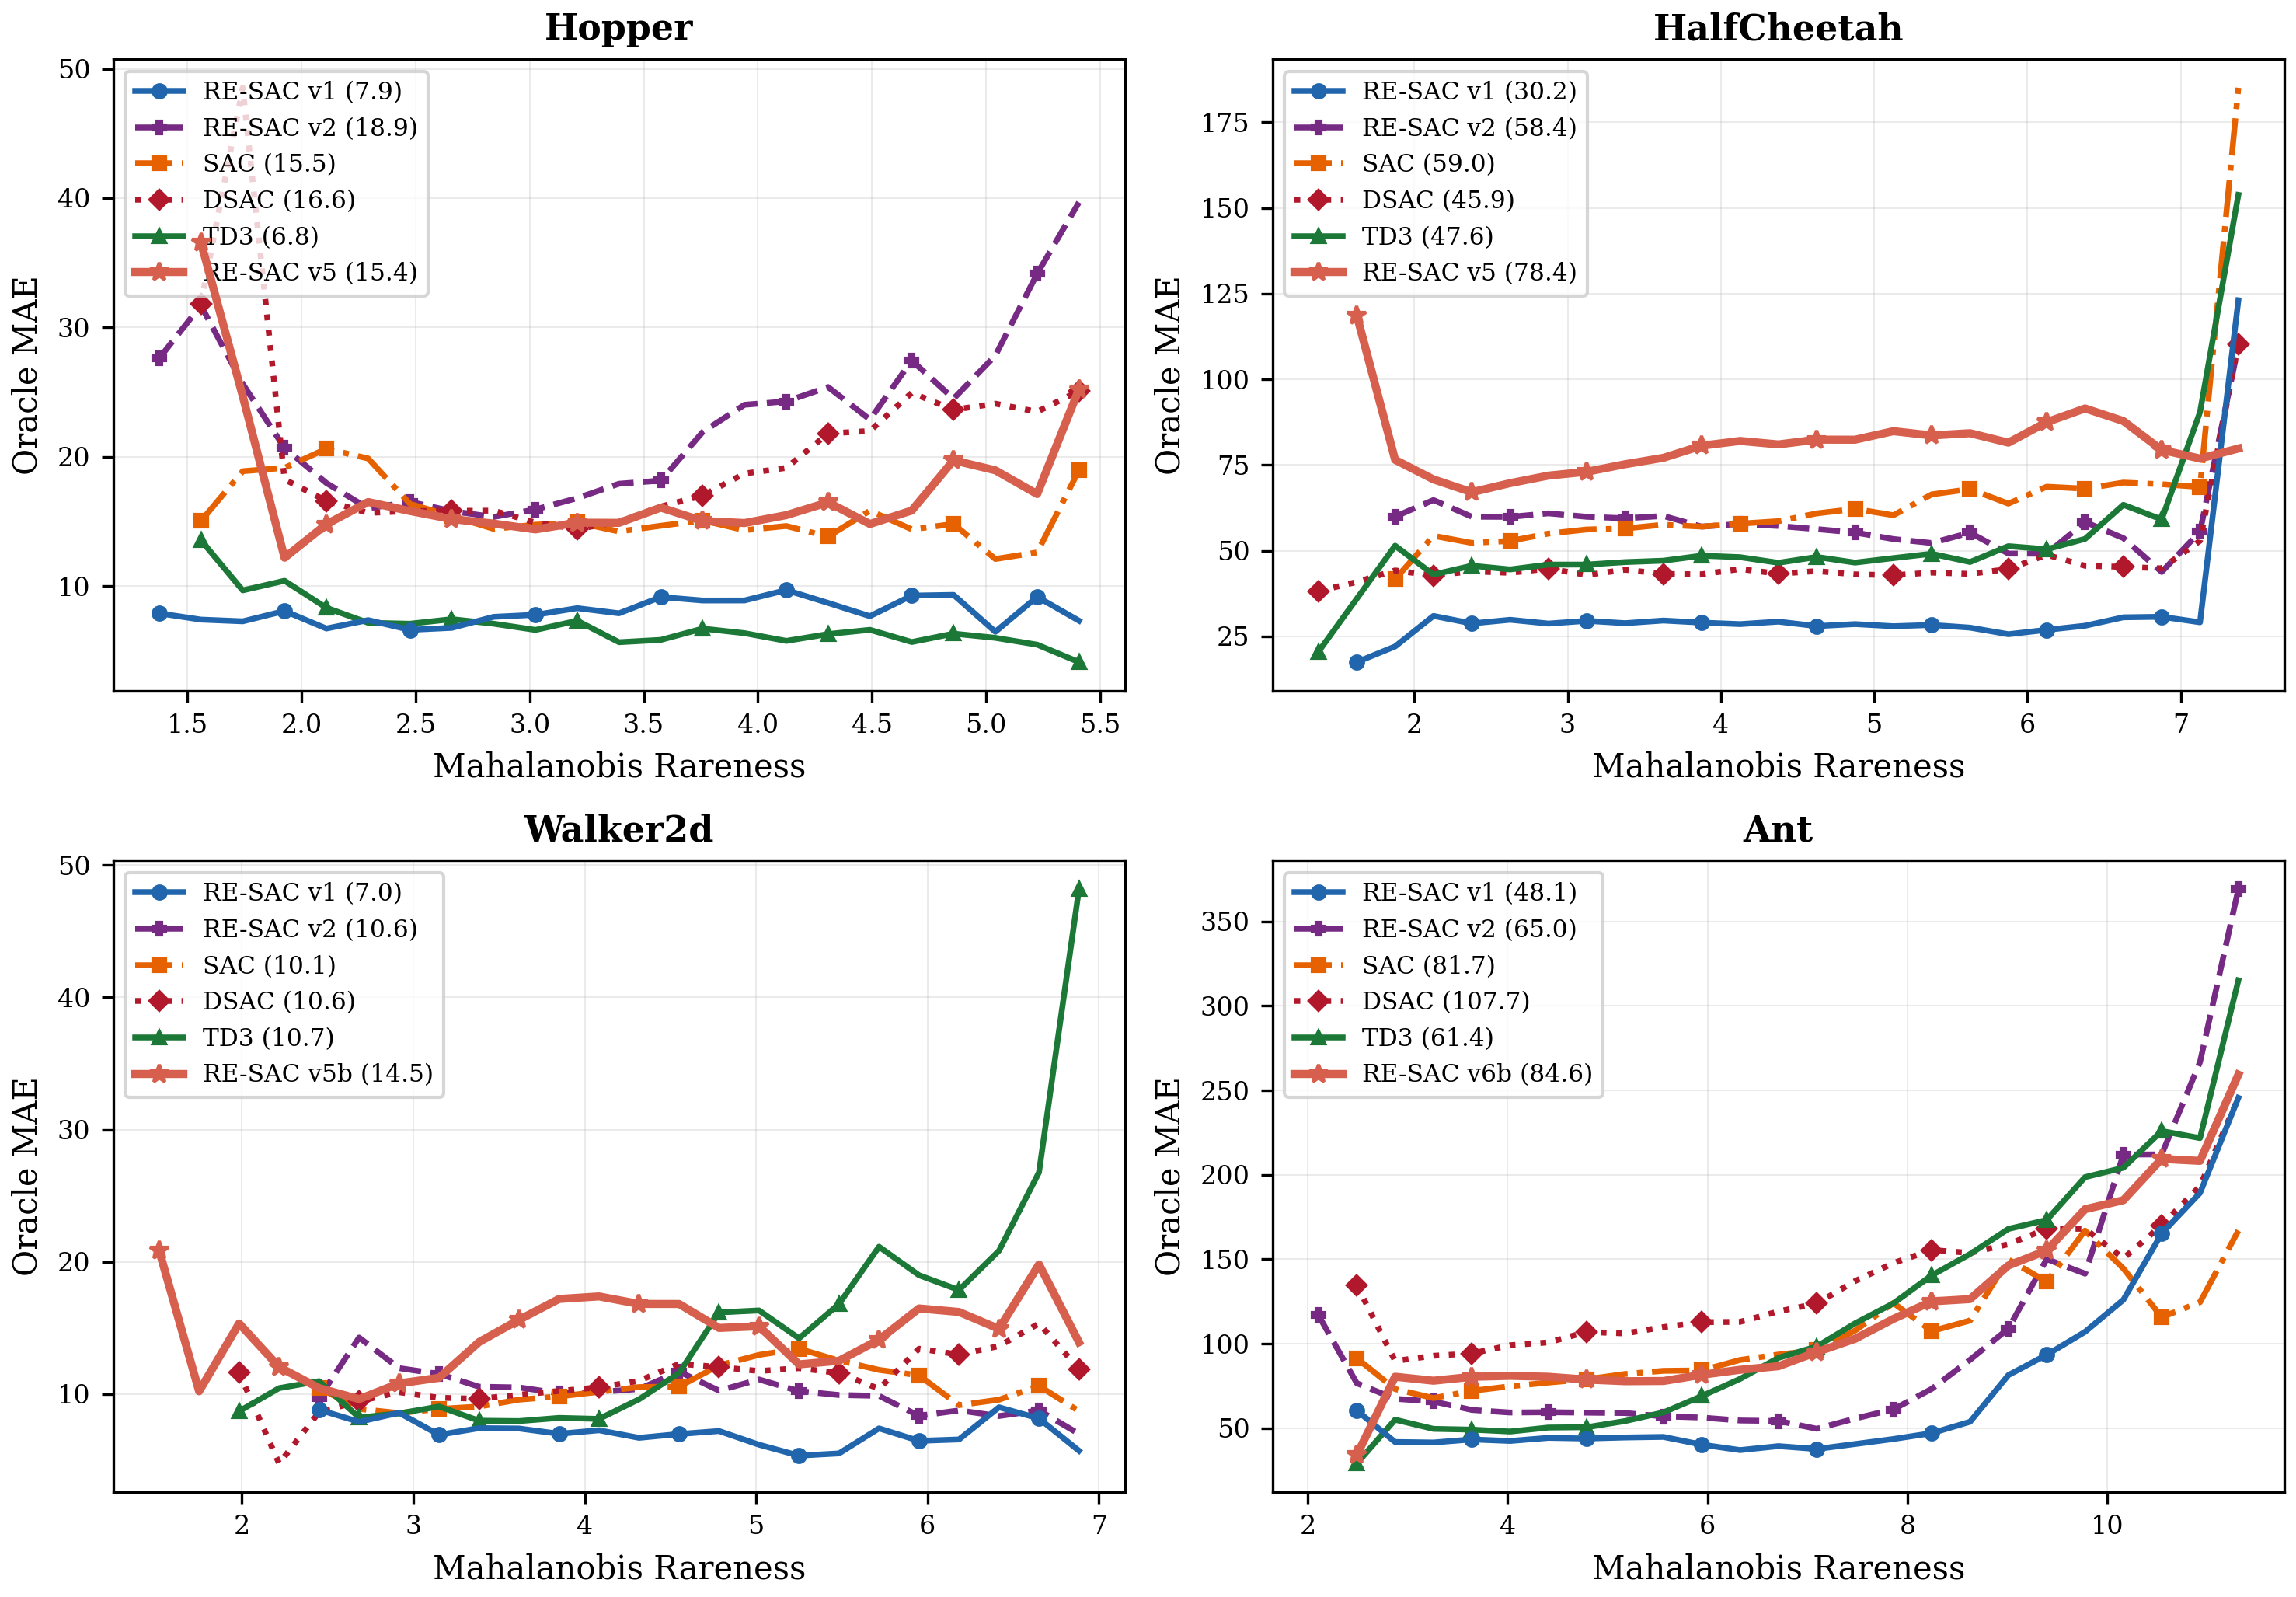
\includegraphics[width=\linewidth]{mujoco_oracle_q_error.png}
    \caption{Oracle Q-Error (MAE) binned by Mahalanobis rareness on four MuJoCo environments. Legend entries show overall Oracle MAE. RE-SAC v1 (solid blue) maintains the lowest estimation error in OOD regions; RE-SAC v5/v6b (red, starred) trades per-head accuracy for ensemble diversity that drives superior policy performance.}
    \label{fig:mujoco_oracle}
\end{figure}

\subsubsection{Training performance}
Fig.~\ref{fig:mujoco_curves} shows evaluation returns during training. RE-SAC v5 (thick red line, per-env best config) achieves the highest final return on all four environments: HalfCheetah 22711 (54\% above SAC), Walker2d 1008 (3.2$\times$ SAC, 2.2$\times$ DSAC), Hopper 660 (above SAC's 645), and Ant 27104 (v6b, surpassing DSAC's 25118). These gains stem from the independent target design preserving ensemble diversity: with meaningful Q-std, the adaptive $\beta_{lcb}$ schedule effectively balances exploration early (pessimistic $\beta{=}{-2}$) and exploitation later ($\beta \to -1$), while the EMA actor and policy anchor prevent the late-training instabilities observed in ablations without these mechanisms.

\begin{figure}[!htbp]
    \centering
    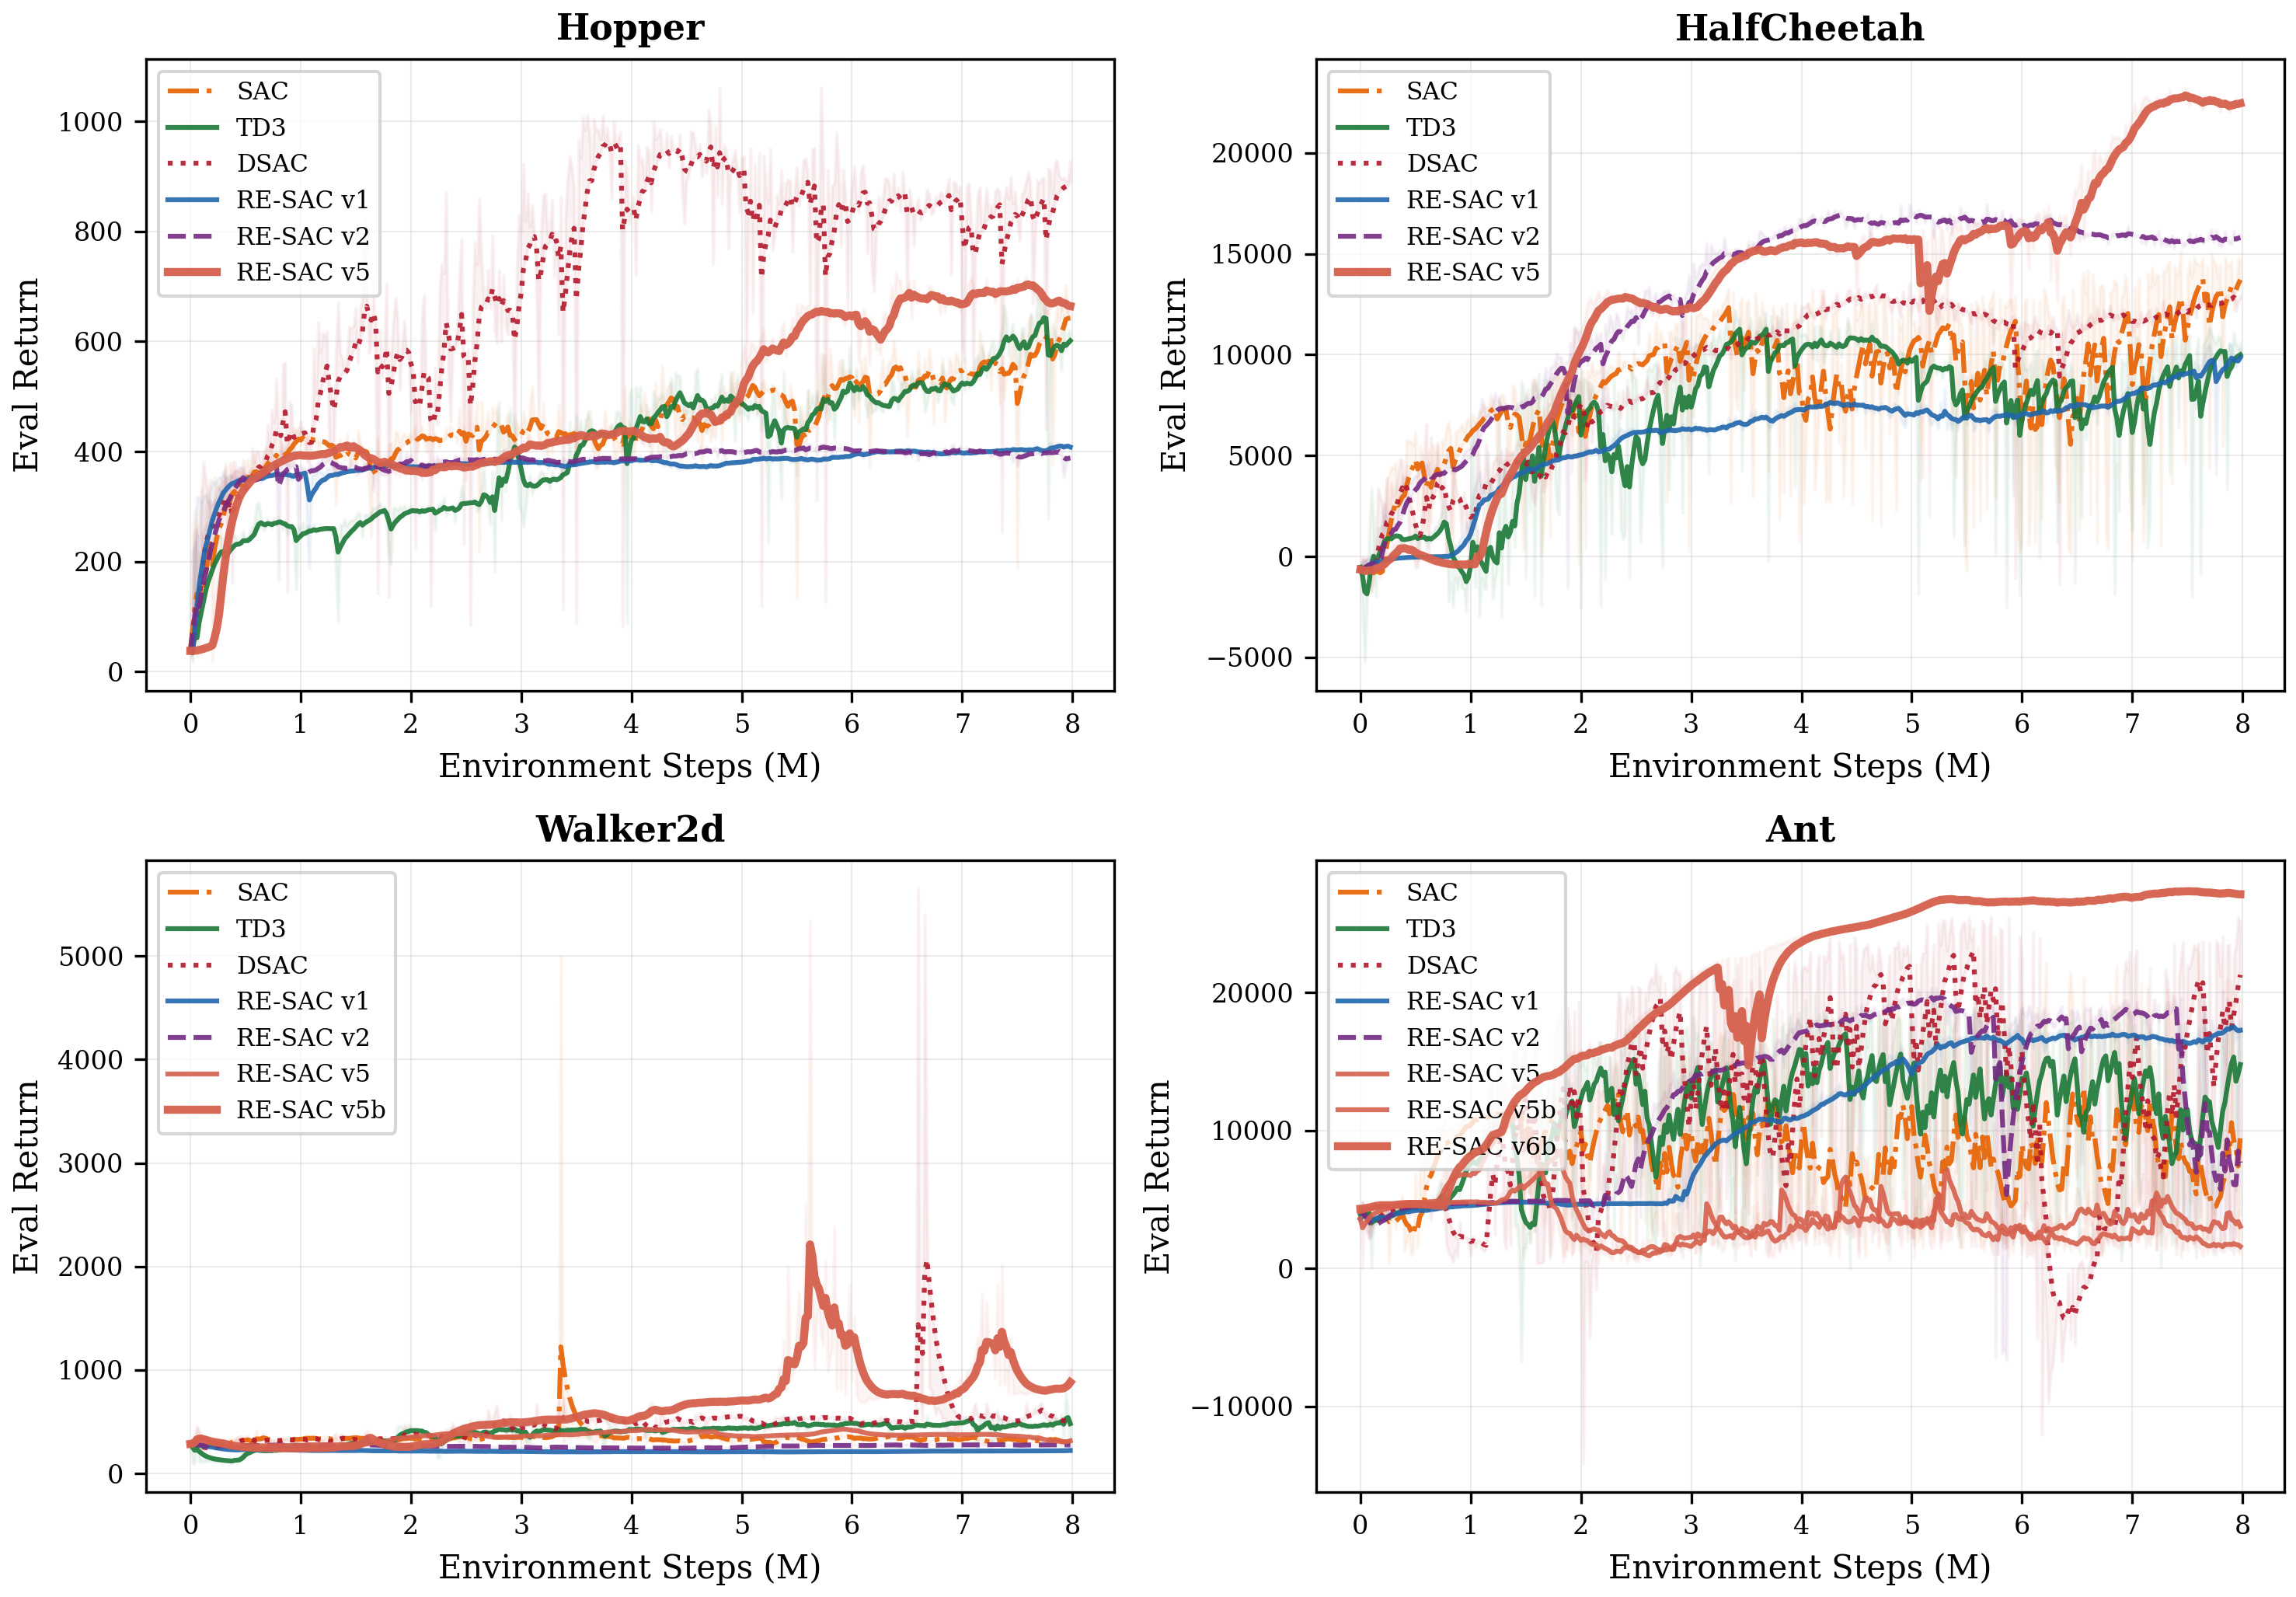
\includegraphics[width=\linewidth]{mujoco_training_curves.png}
    \caption{Evaluation returns on MuJoCo benchmarks (8M steps, seed 8). RE-SAC v5 (thick red) achieves the highest final return on all four environments by maintaining ensemble diversity through independent critic targets.}
    \label{fig:mujoco_curves}
\end{figure}

\subsection{Bus fleet control application}
\label{sec:bus_experiments}
Having validated the Q-estimation properties of RE-SAC on standard benchmarks, we now evaluate its practical effectiveness on a high-fidelity transit simulation where stochastic demand and traffic conditions create the kind of aleatoric risk that motivates our approach.

\subsubsection{Simulation environment}
We evaluate all algorithms on the bidirectional bus corridor simulation developed in our previous work~\cite{Zhang2025SingleAgentBus}. The environment models a realistic timetabled bus line with 22 stops (including two terminals) operating over a 13-hour service window (06:00--19:00). Buses are dispatched every 360 seconds from both terminals with a 180-second directional offset. Upon completing a trip, each vehicle becomes idle at its terminal and is available for reassignment according to the timetable, thereby modeling dynamic fleet sizing.

\textbf{Passenger demand} is specified by an hourly origin-destination (OD) matrix. For each pair of stations and each time period, passenger arrivals are sampled from a Poisson distribution with the corresponding time-varying rate. \textbf{Traffic conditions} are modeled as stochastic inter-stop travel speeds sampled from Gaussian distributions with hourly varying means and a fixed standard deviation of $\sigma = 1.5$~m/s, capturing realistic congestion fluctuations.

\textbf{MDP formulation.} The holding control problem is formulated as an event-driven MDP~\cite{Zhang2025SingleAgentBus}. Decisions are triggered after all passenger boarding/alighting activities have completed at each stop. The \textit{state} $s_t$ consists of categorical features (Bus~ID, Station~ID, Direction, Time~Period) and continuous features (forward headway $h_f$, backward headway $h_b$, current segment speed $v$). The \textit{action} $a_t \in [0, H_{max}]$ specifies the additional holding time at the current stop. The \textit{reward} follows the ridge-shaped function designed in~\cite{Zhang2025SingleAgentBus}, which simultaneously incentivizes headway regularity ($h_f \approx h_b \approx \tau$) and penalizes extreme deviations from the scheduled headway $\tau$.

\subsubsection{Network architecture and hyperparameters}
All algorithms are implemented in PyTorch. The $K$ critic networks are implemented as a single vectorized module (VectorizedCritic) for computational efficiency, each consisting of a 4-layer MLP with hidden dimensions $[64, 64, 64]$ and ReLU activations. The actor network is a separate 4-layer MLP with the same hidden dimension, outputting mean and log-standard-deviation for a squashed Gaussian policy. Following~\cite{Zhang2025SingleAgentBus}, categorical features (Bus~ID, Station~ID, Direction, Time~Period) are encoded via learnable embedding layers with dimension $d = \min(50, \lfloor N_i / 2 \rfloor)$, where $N_i$ is the number of unique categories. The embedded representations are concatenated with continuous state features (forward headway, backward headway, segment speed) to form the input vector.

Key hyperparameters are summarized as follows:
\begin{itemize}
    \item Ensemble size: $K \in \{2, 5, 10, 20, 40\}$ (default $K = 10$ unless otherwise specified);
    \item Learning rate: $1 \times 10^{-5}$ for critic, actor, and temperature (Adam optimizer);
    \item Batch size: 2048;
    \item Replay buffer size: $1 \times 10^6$ transitions;
    \item Discount factor: $\gamma = 0.99$;
    \item Target network smoothing coefficient: $\tau = 0.01$;
    \item Aleatoric regularization coefficient: $\lambda_{ale} = 0.01$ ($\ell_1$ weight penalty in critic target and loss; cf.\ Eq.~8);
    \item Actor LCB weight: $\beta_{lcb} = -2$ (applied as $\bar{Q} + \beta_{lcb} \cdot \sigma_{ens}$ in the actor objective; cf.\ Eq.~14);
    \item OOD penalty coefficient: $\beta_{ood} = 0.01$ (penalizes ensemble standard deviation in critic loss; cf.\ Eq.~12);
    \item Entropy temperature $\alpha$: automatically tuned via dual gradient descent with target entropy $\mathcal{H}_{target} = -\dim(\mathcal{A})$, capped at $\alpha_{\max} = 0.6$;
    \item Gradient clipping: max norm $= 1.0$;
    \item Critic-to-actor update ratio: $2:1$.
\end{itemize}
All baseline algorithms (SAC, DSAC, BAC) share the same network architecture, learning rate, and buffer configuration for fair comparison. Each experiment is trained for 500 episodes with training updates triggered every 5 environment steps, and evaluation metrics are averaged over 10 independent rollouts.

\subsubsection{Baselines and ablations}
To comprehensively evaluate our proposed method, we compare RE-SAC against state-of-the-art baselines and perform ablation studies to isolate the impact of our risk disentanglement.
\begin{itemize}
    \item \textbf{Vanilla SAC}~\cite{Haarnoja2018SAC}: The standard Soft Actor-Critic algorithm without explicit robust regularization or ensemble pessimism.
    \item \textbf{DSAC}~\cite{Ma2025DSAC}: Distributional Soft Actor-Critic, a risk-sensitive variant that learns the continuous return distribution to handle environmental stochasticity.
    \item \textbf{BAC}~\cite{Ji2024SeizingSerendipity}: BEE Actor-Critic~\cite{Ji2024SeizingSerendipity}, an off-policy actor-critic that exploits past successful experiences via the Blended Exploitation and Exploration (BEE) operator to avoid catastrophic value underestimation. We abbreviate it BAC (BEE Actor-Critic) throughout for brevity.
    \item \textbf{Epistemic only (ablation)}: A variant of RE-SAC that only applies the ensemble variance penalty $\Gamma_{epi}$, omitting the aleatoric weight regularization.
    \item \textbf{Aleatoric only (ablation)}: A variant that only applies the IPM-based weight regularization $\Gamma_{ale}$, omitting the ensemble.
\end{itemize}
For RE-SAC, we also evaluate the effect of the ensemble size $K \in \{2, 5, 10, 20, 40\}$.

\subsubsection{Overall performance and learning stability}
Fig.~\ref{fig:all_experiments} displays the smoothed cumulative rewards over training. Vanilla SAC and the Aleatoric-Only ablation suffer from suboptimal convergence, plateauing around a reward of $-0.55 \times 10^6$. The purely distributional baseline, DSAC-v1, performs slightly better but still falls short of the proposed method. Notably, the Epistemic-Only variant experiences a complete catastrophic collapse mid-training, dropping to $-1.2 \times 10^6$. This confirms our hypothesis: relying solely on ensemble variance in a highly stochastic environment misidentifies inherent noise as missing data, leading to runaway pessimism and policy degradation.

By successfully disentangling the uncertainties, RE-SAC (particularly with moderate ensemble sizes $K=5, 10, 20$) achieves the highest and most stable final reward (around $-0.4 \times 10^6$). Excessively large ensembles ($K=40$) show a slight performance degradation: with 40 parallel critics, the accumulated variance penalty $\lambda_{epi}\Gamma_{epi}$ becomes more sensitive to transient disagreements during early training, inducing a conservative bias that persists and slightly suppresses the final reward. This is consistent with the known over-pessimism of large ensembles in online settings~\cite{An2021UncertaintyEnsemble}. 
The BAC baseline, designed to avoid underestimation by exploiting past successes, performs relatively well but exhibits higher variance during training compared to RE-SAC, settling at a slightly lower final reward than the best RE-SAC variants. This suggests that while maintaining optimistic estimates of past serendipitous events helps avoid complete policy collapse in stochastic environments, explicitly disentangling and regularizing against aleatoric and epistemic risks provides a more stable and robust policy improvement path.

\begin{figure}[!htbp]
    \centering
    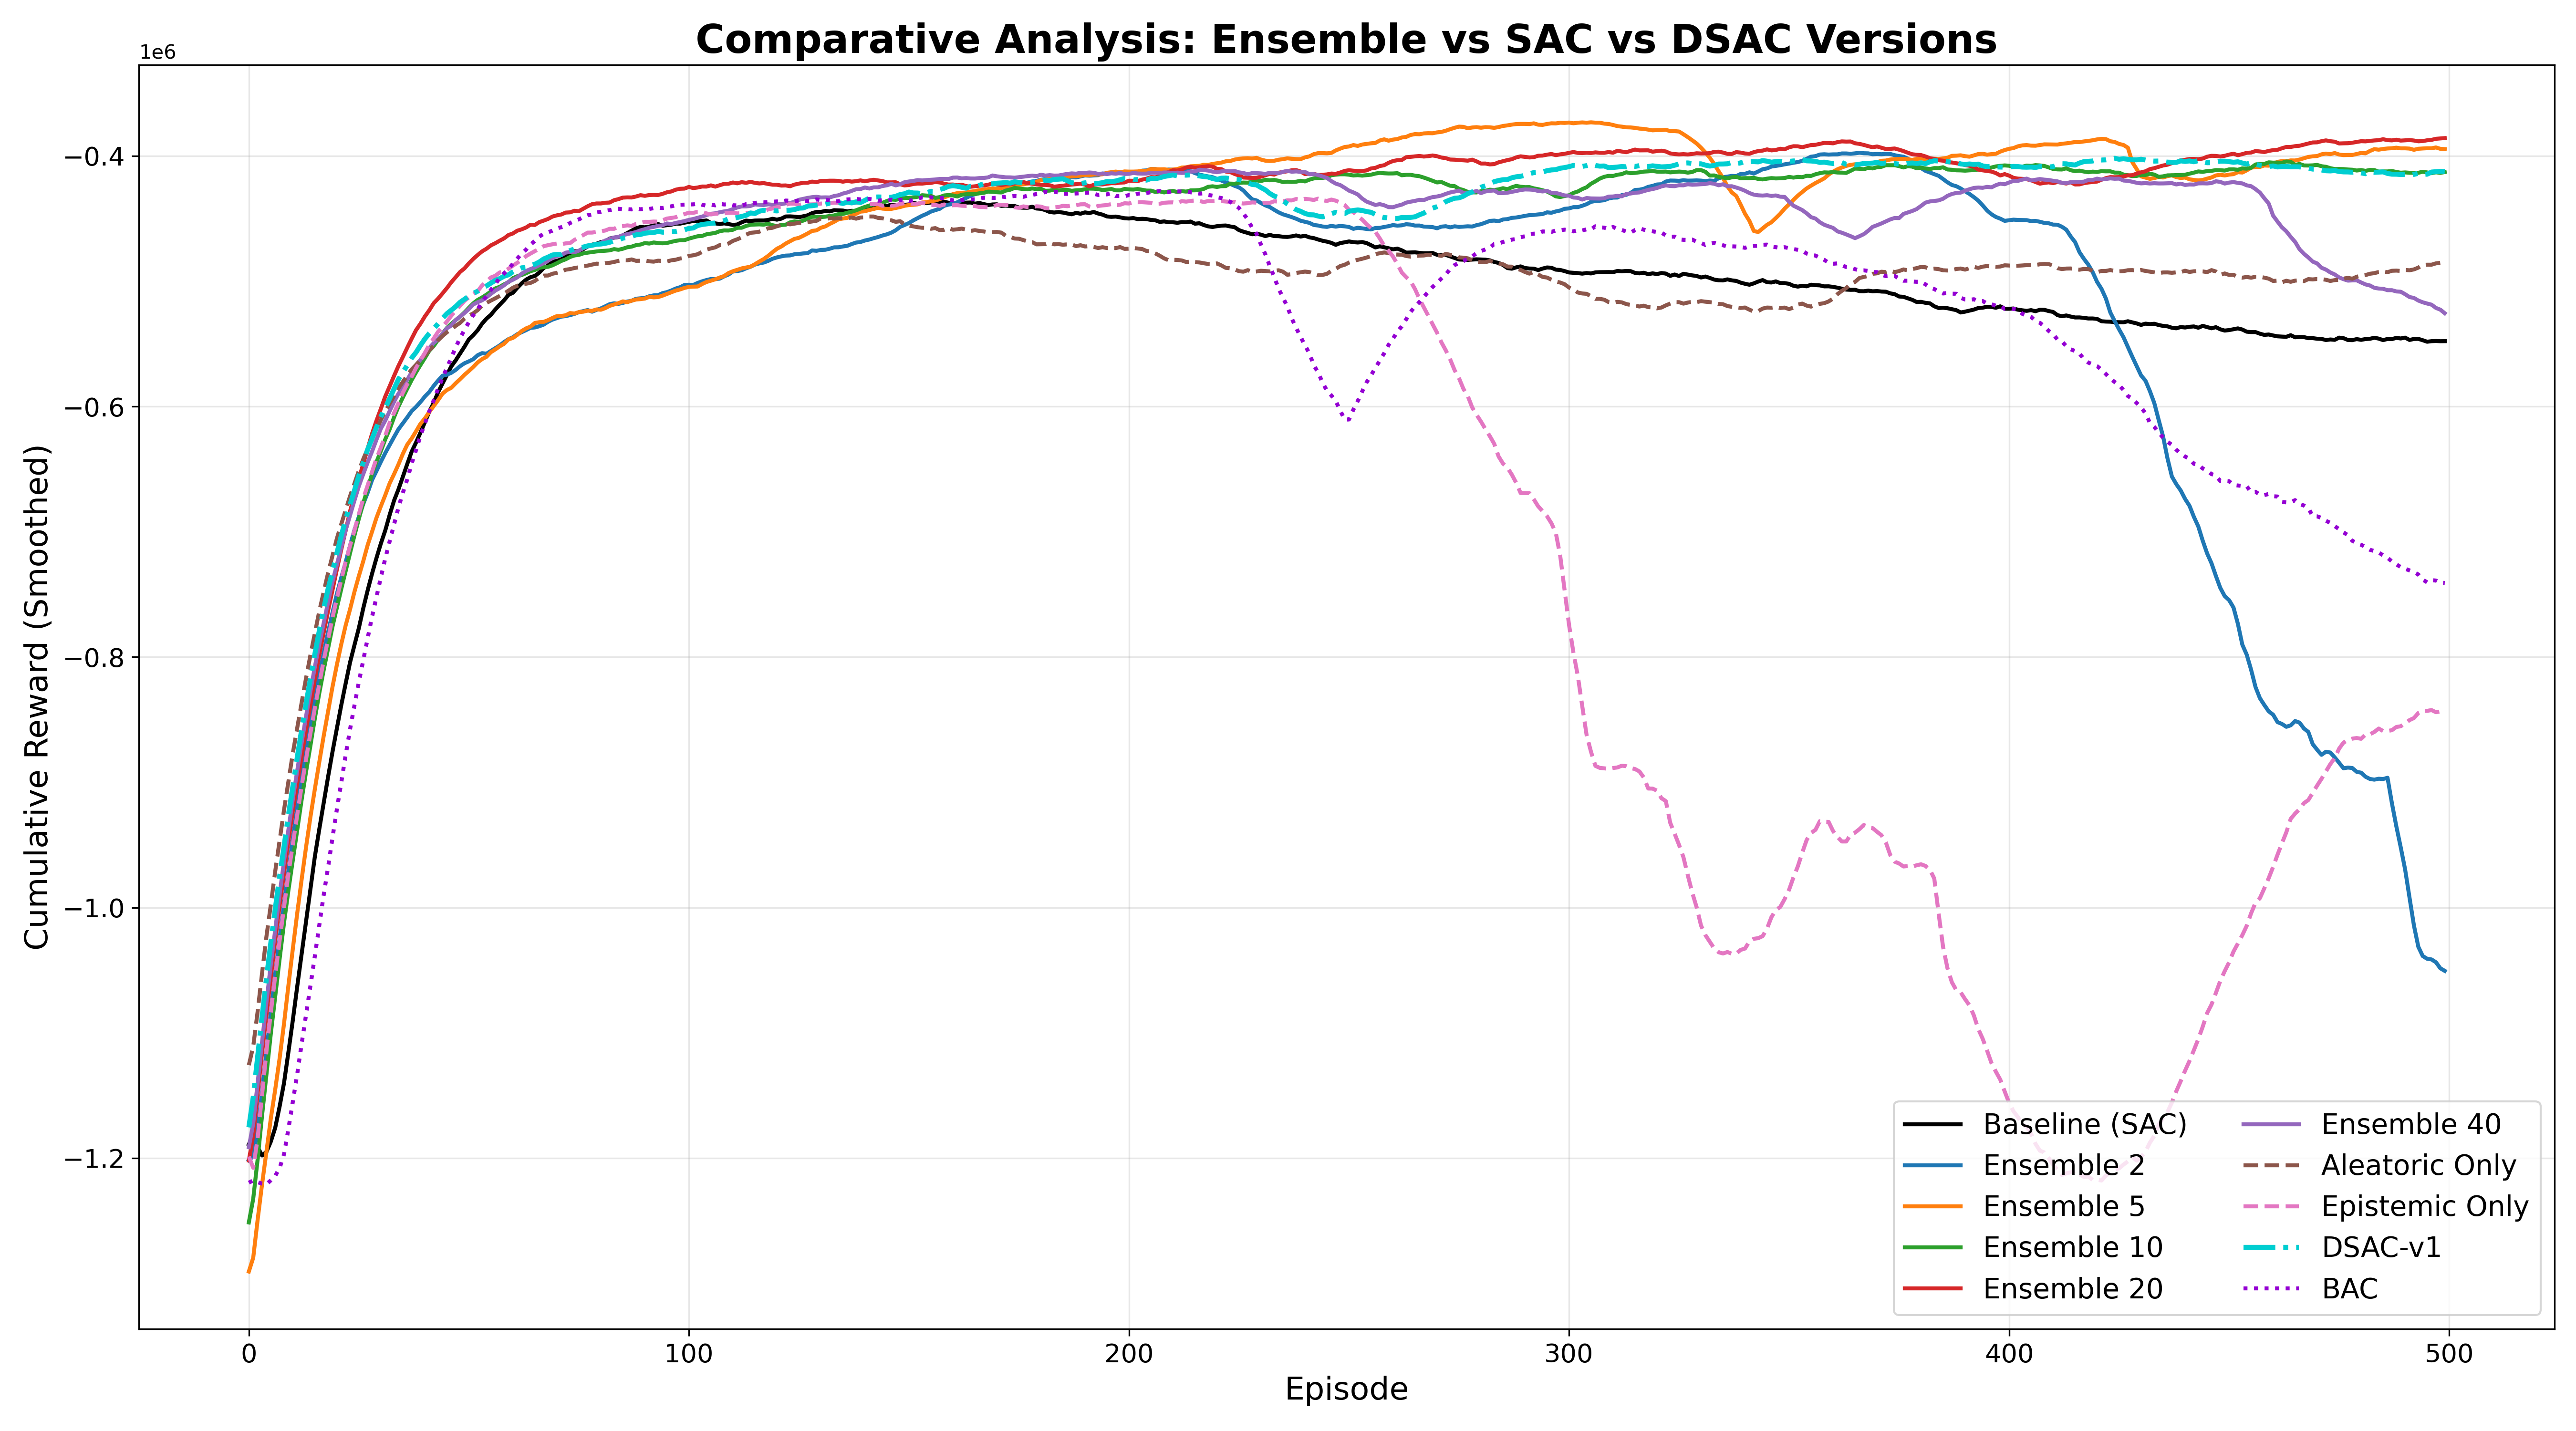
\includegraphics[width=\linewidth]{all_experiments_comparison_v2.png}
    \caption{Learning curves of cumulative reward for RE-SAC variants, SAC, DSAC-v1, BAC, and ablations.}
    \label{fig:all_experiments}
\end{figure}

\subsubsection{Q-value estimation stability}
The catastrophic drop in the Epistemic-Only policy is directly correlated with extreme value underestimation. As shown in Fig.~\ref{fig:all_q_values}, the estimated Q-values for the Epistemic-Only ablation plummet deep into negative values (passing $-3000$) with a massive $2\sigma$ variance band, corroborating the ``underestimation trap''. In contrast, RE-SAC variants and baseline SAC maintain relatively stable Q-value ranges. The disentangled penalties in RE-SAC prevent the variance penalty from overwhelming the nominal expected return.

\begin{figure}[!htbp]
    \centering
    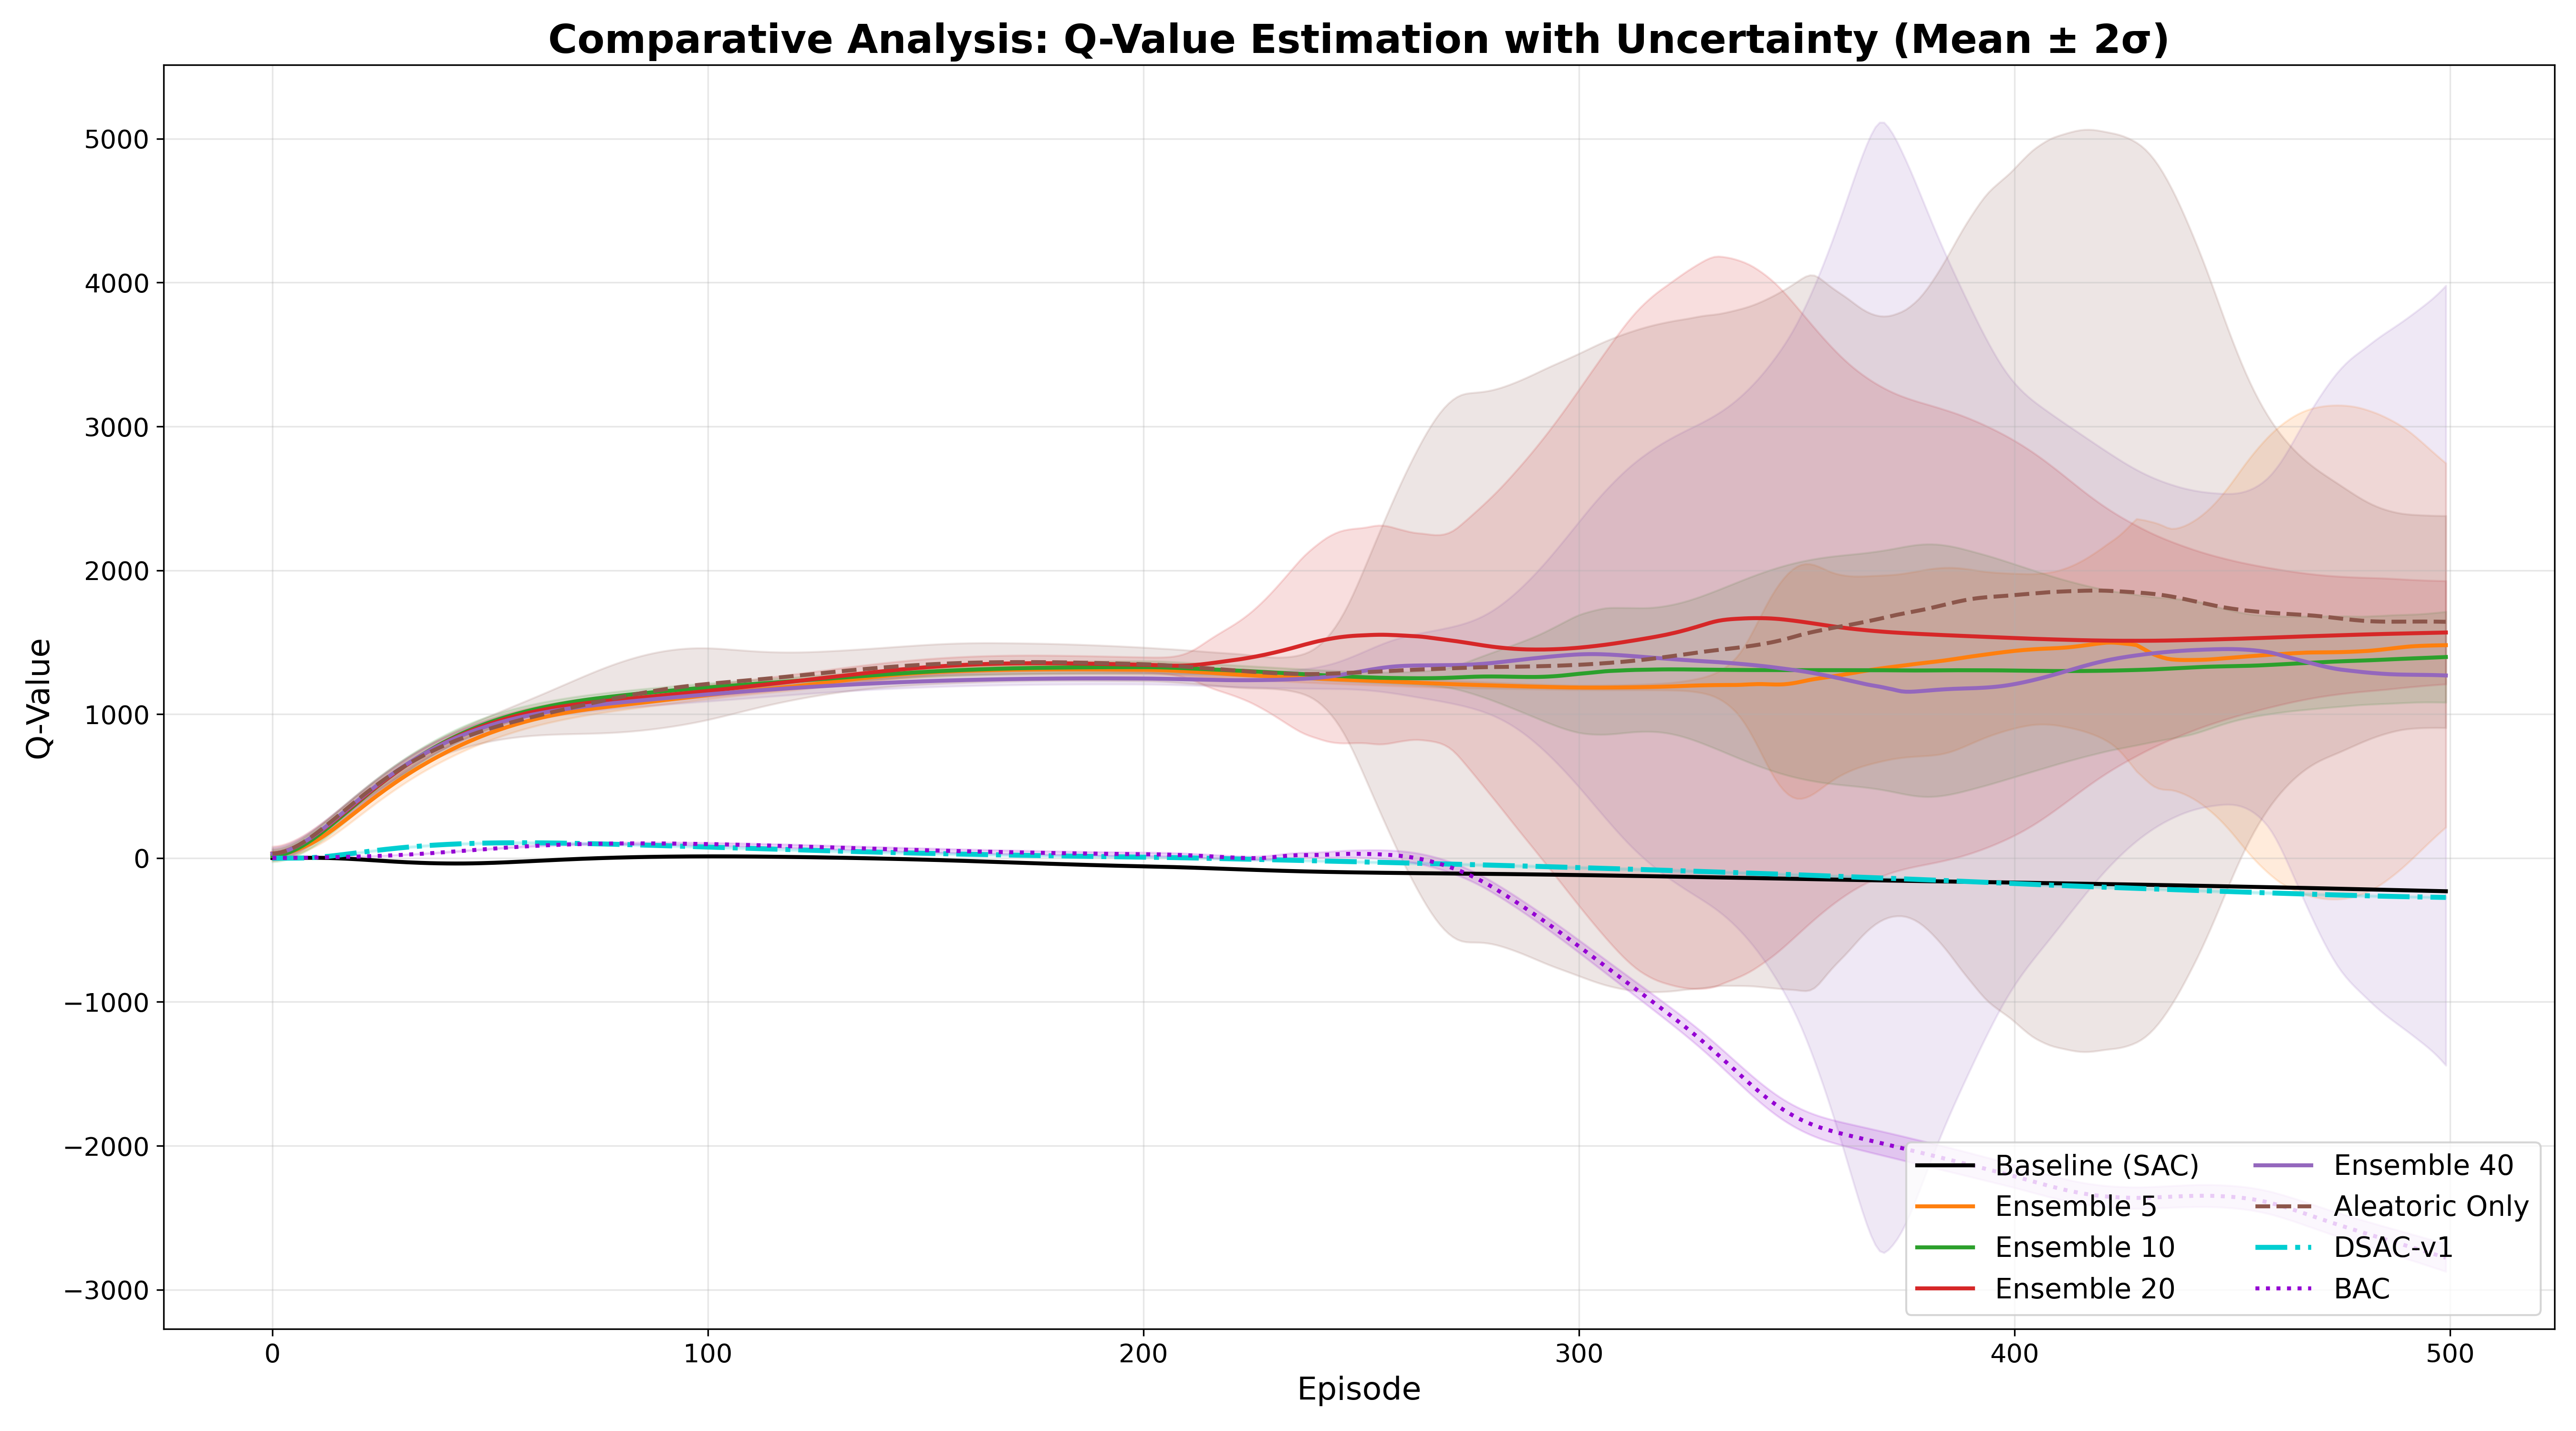
\includegraphics[width=\linewidth]{all_q_values_comparison_v2.png}
    \caption{Comparative analysis of estimated Q-Values (Mean $\pm$ $2\sigma$) over training.}
    \label{fig:all_q_values}
\end{figure}

\subsubsection{Robustness in rare states (Mahalanobis rareness)}
While the preceding Q-value analysis tracks estimation stability \emph{over training episodes}, a robust optimization perspective demands a complementary view: \emph{at the same level of state rarity, does the algorithm produce smaller estimation errors than baselines?} This distinction is essential because robust policies are valued not for their average-case accuracy, but for their ability to maintain bounded estimation errors in the worst-case regions of the state space.

To formalize this, we define \textbf{Mahalanobis rareness}. The key design choices are as follows. First, we condition on each \emph{spatial-directional group} (Station~ID $\times$ Direction), because different stops exhibit fundamentally different nominal headway distributions---for example, departure headways at terminals are tightly constrained by the timetable, whereas mid-route headways are subject to cumulative disturbances. A single global distribution would conflate structurally different operating regimes. For each group, we fit a 2D Gaussian to the observed continuous features (Forward Headway, Backward Headway), estimating the empirical mean $\mu$ and covariance $\Sigma$. Second, we use the \emph{Mahalanobis distance} rather than a simple Euclidean norm because the two headway features have different scales and are correlated (e.g., a very large forward headway typically co-occurs with a small backward headway in a bunching event). Euclidean distance is sensitive to these scale differences and ignores feature correlations, whereas the Mahalanobis distance $\sqrt{(x-\mu)^T\Sigma^{-1}(x-\mu)}$ naturally normalizes by the feature covariance, so that equally likely headway combinations receive equal rareness scores regardless of their direction in feature space. Intuitively, a state with high Mahalanobis rareness is one whose headway configuration the agent has rarely encountered at that stop during training---precisely the kind of state where epistemic risk is highest.

Fig.~\ref{fig:mahalanobis} bins the Mean Absolute Error (MAE) between each algorithm's Q-value estimates and the ground-truth Monte Carlo return $Q_{MC}(s,a)$ by Mahalanobis rareness. Here, $Q_{MC}$ is computed offline from the recorded evaluation trajectories as the discounted cumulative reward from each decision point onward: $Q_{MC}(s_t, a_t) = \sum_{k=0}^{T-t} \gamma^k r_{t+k}$, providing a model-free ground truth independent of any learned value function.

Since different algorithms learn Q-values at different absolute scales, direct comparison of raw prediction errors would be misleading. We therefore apply a per-algorithm z-score alignment that rescales each algorithm's predictions to match the mean and standard deviation of $Q_{MC}$ before computing the error. Additionally, for ensemble-based algorithms, we report the \textbf{Oracle MAE}: for each state, we select the ensemble head whose aligned prediction is closest to $Q_{MC}$, and compute the MAE over these best-head predictions. This oracle serves as a favorable upper bound on the ensemble's representational capacity---it measures how well the ensemble \textit{could} estimate the true return if paired with an ideal head-selection mechanism.

As states become increasingly rare (moving left to right on the x-axis), the estimation errors for Vanilla SAC and DSAC-v1 escalate significantly, confirming that their value networks extrapolate unreliably outside the training distribution. In contrast, RE-SAC (Ensemble) consistently demonstrates the lowest Oracle MAE across all rareness bins (overall average of 1647, compared to SAC's 4343 and DSAC's 5945). The tight error bands around the RE-SAC predictions confirm that the disentangled regularization structurally bounds the value network, preventing wild extrapolations in OOD regions and yielding superior worst-case guarantees.
\vspace{-2pt}
\begin{figure}[!htbp]
    \centering
    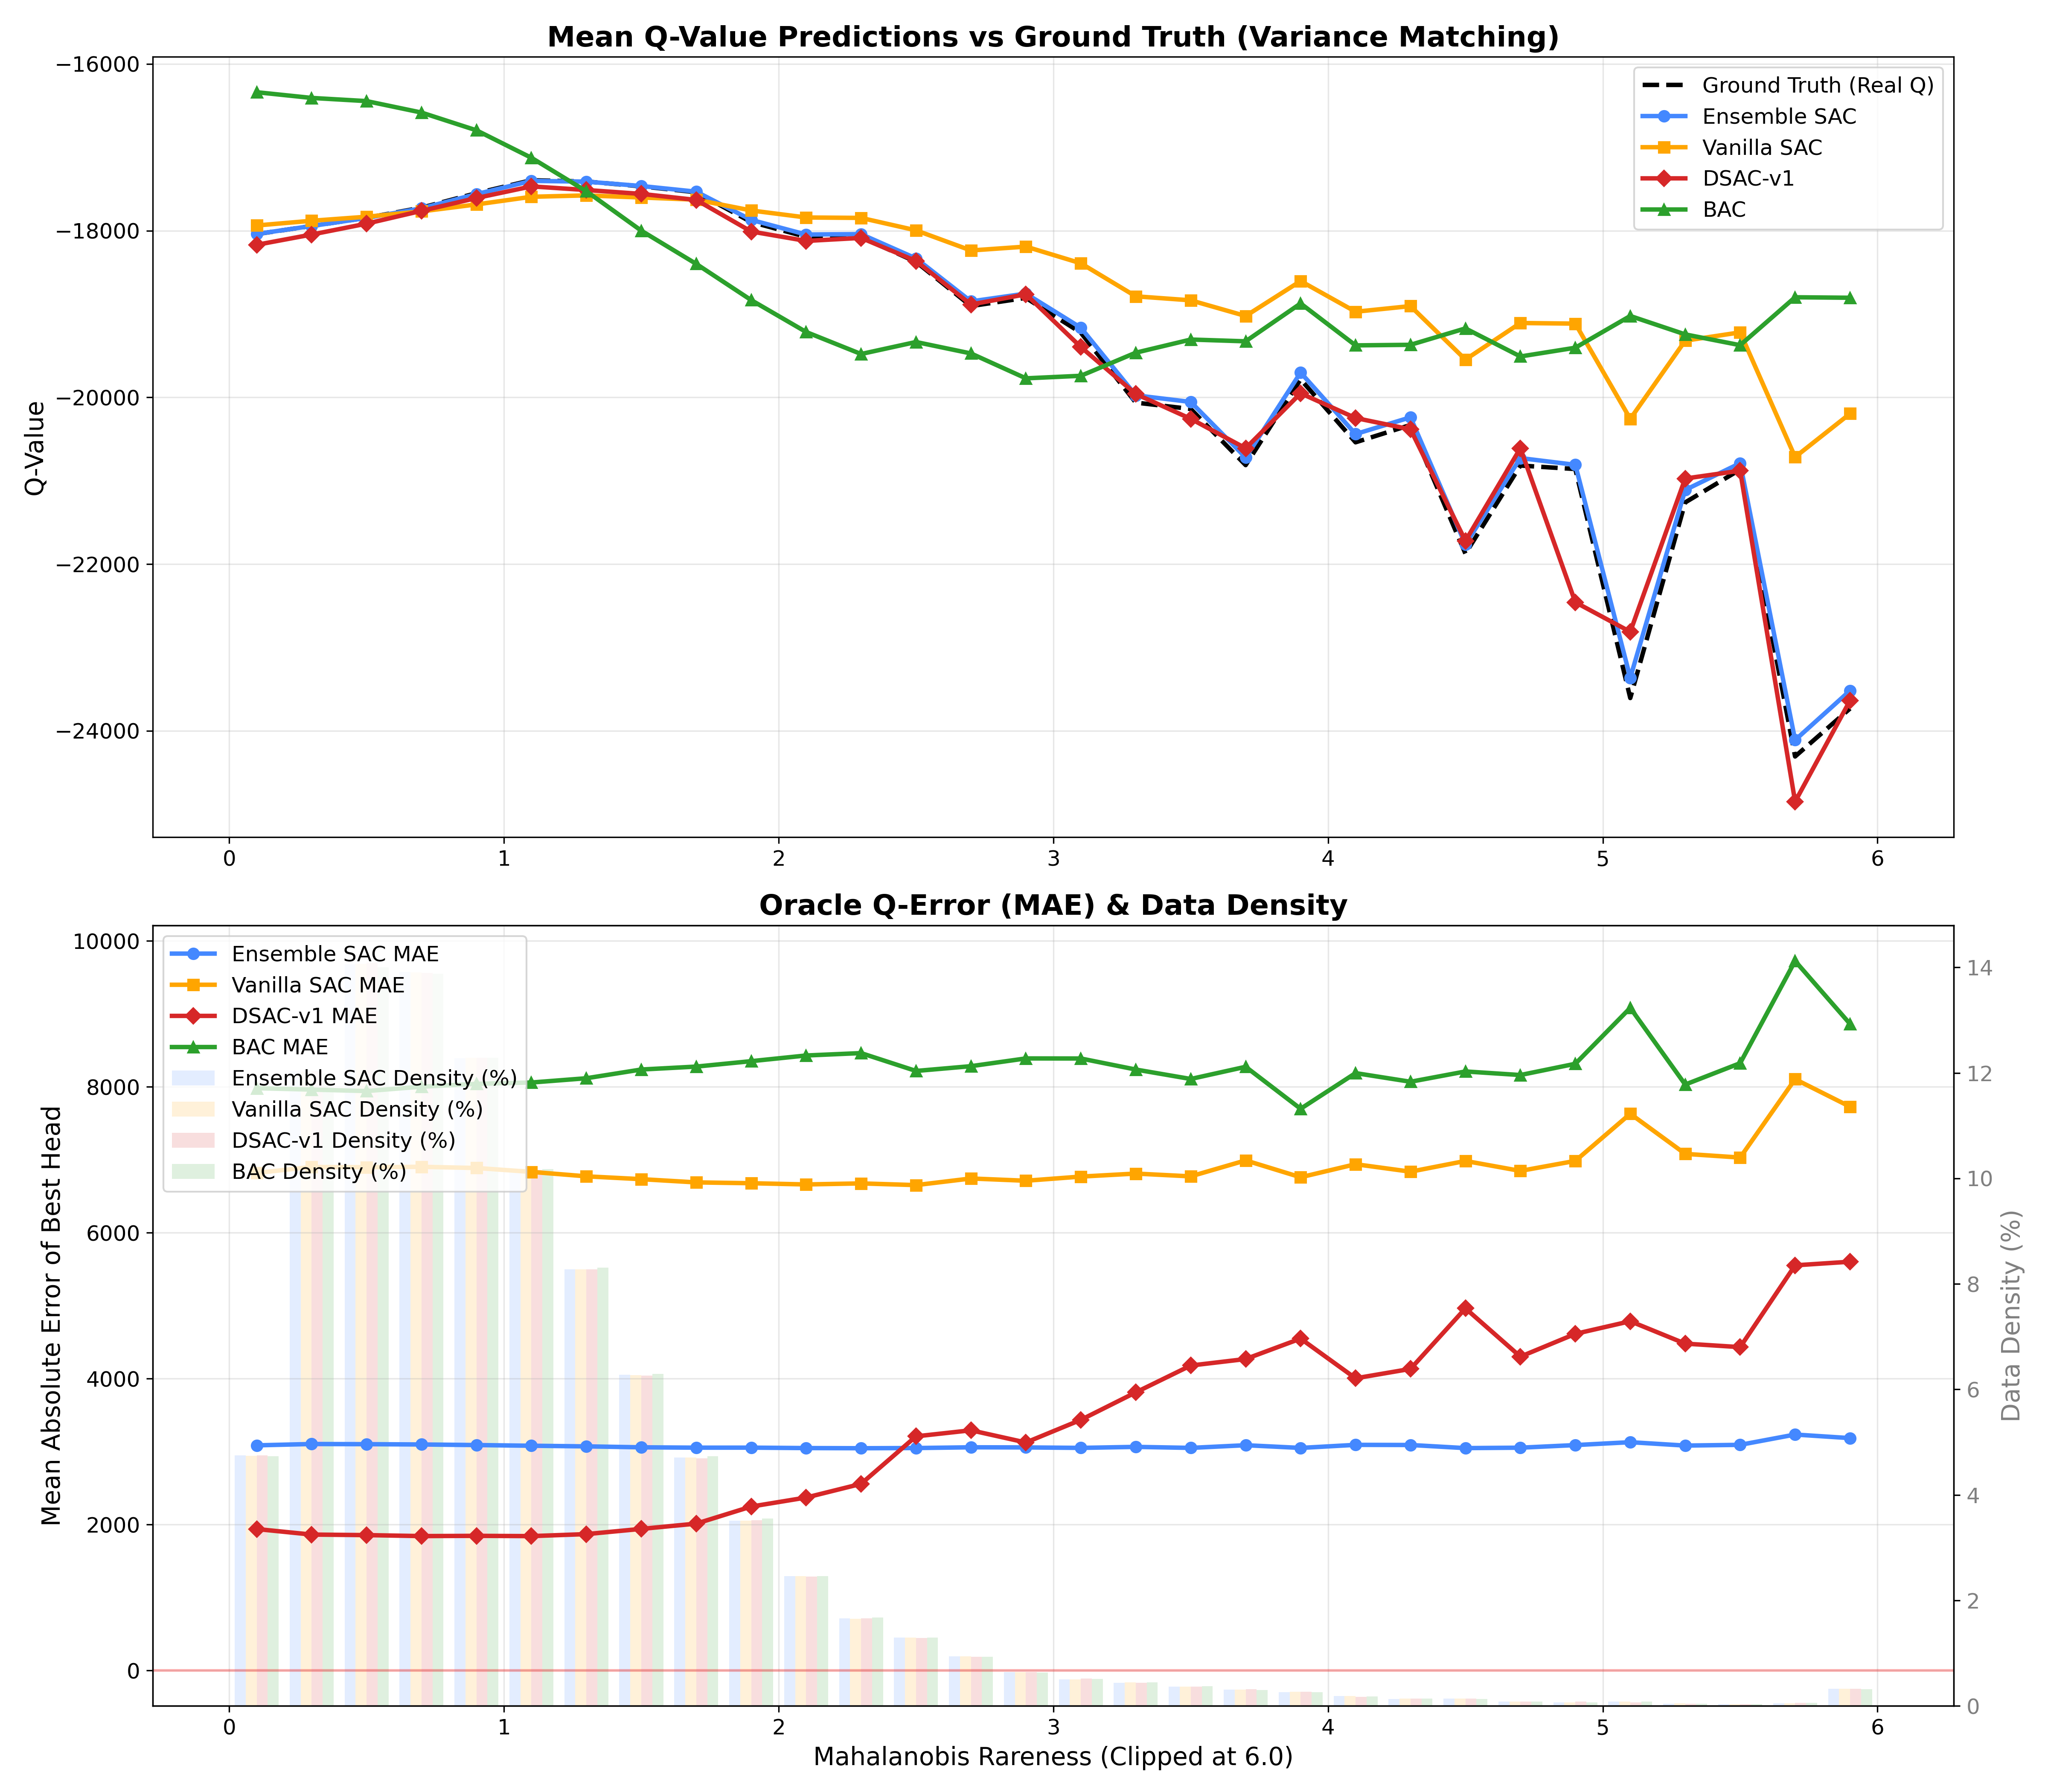
\includegraphics[width=\linewidth]{comparison_mahalanobis_rareness_restyled.png}
    \vspace{-6pt}
    \caption{Oracle Q-Error (MAE) banded by Mahalanobis Rareness. RE-SAC maintains accurate estimates even in highly rare/OOD states.}
    \label{fig:mahalanobis}
\end{figure}

\FloatBarrier
\section{Conclusion}
This paper presents the RE-SAC framework, a robust reinforcement learning approach that explicitly disentangles aleatoric and epistemic uncertainties. Grounded in the theoretical correspondence between risk-sensitivity and robustness established by Osogami~\cite{Osogami2012Robustness}, our method employs two complementary mechanisms: IPM-based weight regularization to enforce Lipschitz continuity of the value function against inherent environmental stochasticity, and a diversified $Q$-ensemble to penalize overconfident estimates in data-sparse regions of the state-action space.

Our theoretical analysis identifies a sharp structural boundary for contraction in multi-penalty Bellman operators: the frozen-parameter design (target networks for epistemic variance, held-fixed critic weights for aleatoric penalty) is both sufficient for $\gamma$-contraction and \emph{necessary}---Q-dependent penalties provably break it.  Both results are machine-verified in Lean~4 with no \texttt{sorry}, and a verifiable feasibility condition on the penalty coefficients guarantees policy non-degeneration (Appendix~\ref{app:nondegen}).  This structural insight---that the standard deep RL architecture of frozen target networks is not merely a stabilisation heuristic but a \emph{required} condition for operator contractiveness---may inform the design of future multi-penalty RL algorithms.

Empirically, on standard MuJoCo benchmarks, RE-SAC achieves the lowest Oracle Q-estimation error on 3 of 4 environments, reducing MAE by up to 55\% relative to DSAC and 41\% relative to SAC on the high-dimensional Ant task. On a realistic bidirectional bus simulation, RE-SAC achieves the highest and most stable cumulative reward among all baselines, including vanilla SAC, DSAC, and BAC. The ablation studies reveal that relying solely on ensemble variance (Epistemic-Only) leads to catastrophic value collapse in high-variance transit environments, while using only weight regularization (Aleatoric-Only) fails to detect out-of-distribution states. The Mahalanobis rareness analysis further confirms that RE-SAC maintains accurate $Q$-value estimates even under highly rare traffic states, exhibiting superior worst-case robustness.

In future work, we plan to extend this framework to multi-line transit networks with transfer coordination, investigate adaptive scheduling of the uncertainty coefficients $\lambda_{ale}$ and $\lambda_{epi}$ during training, and explore the integration of distributional RL methods with our disentangled robustness framework to further improve tail-risk management in urban transit systems.

\section*{Acknowledgments}
This work was supported by the National Natural Science Foundation of China (Grant No. 72371251), the Natural Science Foundation for Distinguished Young Scholars of Hunan Province (Grant No. 2024JJ2080), and the Key Research and Development Program of Hunan Province of China (Grant No. 2024JK2007).

\bibliographystyle{IEEEtran}
\documentclass[10pt]{article}
\usepackage[utf8]{inputenc}
\usepackage[T1]{fontenc}
\usepackage[margin=1in, left=1.25in, right=1.25in, top=1in, bottom=1in]{geometry}
\usepackage{algorithm}
\usepackage{algorithmic}
\usepackage[linktoc=all, bookmarksdepth=3, pdfstartview=FitH]{hyperref}
\hypersetup{colorlinks=true, linkcolor=blue, filecolor=magenta, urlcolor=cyan}
\urlstyle{same}
\usepackage{amsmath}
\usepackage{amsfonts}
\usepackage{amssymb}
\usepackage[version=4]{mhchem}
\usepackage{stmaryrd}
\usepackage{bbold}
\usepackage{graphicx}
\usepackage[export]{adjustbox}
\usepackage[dvipsnames]{xcolor}
\usepackage{float}
\usepackage{placeins}
\usepackage{caption}
\captionsetup[figure]{name=Fig.}
\usepackage{booktabs}
\usepackage{multirow}
% ==== Revision color macro (keep for marked version) ====
\usepackage[normalem]{ulem} % for \sout
\usepackage{amsthm}
\usepackage{enumitem}
\newtheorem{theorem}{Theorem}[section]
\newtheorem{lemma}[theorem]{Lemma}
\newtheorem{definition}[theorem]{Definition}
\newtheorem{corollary}[theorem]{Corollary}
\newtheorem{proposition}[theorem]{Proposition}
\newtheorem{remark}[theorem]{Remark}
% \newcommand{\revise}[1]{{\color{blue}#1}}
% \newcommand{\del}[1]{\color{red}{\sout{#1}}}             % deletions (red strikeout)
\newcommand{\revise}[1]{#1}
\newcommand{\del}[1]{}

% ==== Algorithm package ====
% Option A: algorithm2e
% \usepackage[ruled,vlined,linesnumbered]{algorithm2e}
% Or Option B: algpseudocode


\graphicspath{ {./} }

\title{RE-SAC: Disentangling aleatoric and epistemic risks in bus fleet control: A stable and robust ensemble DRL approach\footnote{Code available at \url{https://github.com/erzhu419/RE-SAC}}}

\author{
  Yifan Zhang\thanks{Central South University, \href{mailto:erzhu419@gmail.com}{erzhu419@gmail.com}, \href{mailto:204201048@csu.edu.cn}{204201048@csu.edu.cn}} \and
  Liang Zheng\thanks{Central South University, \href{mailto:zhengliang@csu.edu.cn}{zhengliang@csu.edu.cn}}
}
\date{}


%New command to display footnote whose markers will always be hidden
\let\svthefootnote\thefootnote
\newcommand\blfootnotetext[1]{%
  \let\thefootnote\relax\footnote{#1}%
  \addtocounter{footnote}{-1}%
  \let\thefootnote\svthefootnote%
}

%Overriding the \footnotetext command to hide the marker if its value is `0`
\let\svfootnotetext\footnotetext
\renewcommand\footnotetext[2][?]{%
  \if\relax#1\relax%
    \ifnum\value{footnote}=0\blfootnotetext{#2}\else\svfootnotetext{#2}\fi%
  \else%
    \if?#1\ifnum\value{footnote}=0\blfootnotetext{#2}\else\svfootnotetext{#2}\fi%
    \else\svfootnotetext[#1]{#2}\fi%
  \fi
}

\begin{document}
\maketitle


\begin{abstract}
Bus holding control remains a persistent challenge in urban transit systems due to the inherent stochasticity of traffic conditions and passenger demand. While deep reinforcement learning (DRL) has shown promise for dynamic holding decisions, standard actor-critic algorithms frequently suffer from $Q$-value instability in highly volatile environments. A key yet underexplored source of this instability is the conflation of two structurally distinct uncertainties: \textit{aleatoric} uncertainty, arising from irreducible environmental noise, and \textit{epistemic} uncertainty, arising from data insufficiency in the replay buffer. Treating these as a single risk leads to pathological underestimation in well-explored but noisy states, ultimately causing catastrophic value collapse.

In this paper, we propose a robust ensemble soft actor-critic (RE-SAC) framework that explicitly disentangles and addresses both sources of uncertainty. Our approach applies Integral Probability Metric (IPM)-based weight regularization to the critic network to hedge against aleatoric risk, providing a smooth analytical lower bound for the robust Bellman operator without requiring expensive inner-loop state perturbations. To address epistemic risk, a diversified $Q$-ensemble penalizes overconfident value estimates in sparsely covered regions of the state-action space. This dual mechanism prevents the ensemble variance from misidentifying inherent noise as a data gap, a failure mode that causes complete policy collapse in our ablation study.

Empirically, experiments in a realistic bidirectional bus corridor simulation demonstrate that RE-SAC achieves the highest and most stable cumulative reward (approximately $-0.4 \times 10^6$) among all baselines, compared to $-0.55 \times 10^6$ for vanilla SAC and $-1.2 \times 10^6$ for the epistemic-only ablation. The Mahalanobis rareness analysis further confirms that RE-SAC reduces \emph{Oracle} Q-value estimation error by up to $62\%$ in rare out-of-distribution states relative to SAC (average Oracle MAE of 1647 vs.\ 4343), demonstrating superior worst-case robustness under high traffic variability.
Our theoretical analysis further reveals that the frozen-parameter design (target networks, held-fixed critic weights) is not merely a practical stabilisation heuristic but a \emph{structurally necessary condition} for Bellman operator contractiveness under multi-penalty regularisation---an insight with implications beyond transit control.
\end{abstract}


\noindent\textbf{Keywords:} bus bunching; robust reinforcement learning; ensemble; uncertainty decomposition; bus holding control.


\section{Introduction}

Bus bunching---the phenomenon where multiple buses on the same route cluster together---remains a well-known challenge in urban transit systems. This instability is driven by a positive feedback loop: a slight delay at a stop increases passenger accumulation, which extends dwell time, further slowing the leading bus while the trailing bus speeds up due to reduced demand~\cite{Daganzo2009Headway, Xuan2011Dynamic}. To break this cycle, various holding control strategies have been developed, transitioning from classical schedule-based optimization to deep reinforcement learning (DRL) paradigms~\cite{Wang2020DynamicHolding}.
However, despite the promising performance of DRL in controlled simulations, these models often exhibit fragile behavior when deployed in realistic, high-variance transit environments.

A critical, yet frequently overlooked bottleneck in applying Actor-Critic methods to transit control is what we term ``$Q$-value poisoning.'' In public transportation, stochasticity is not a transient disturbance but a deeply ingrained feature; fluctuations in passenger arrival rates and road traffic speeds are often irreducible. In such highly volatile environments, standard off-policy algorithms like Soft Actor-Critic (SAC) frequently suffer from pathological value estimation degradation. As training progresses, the $Q$-function may become ``poisoned'' by environmental noise, leading to severe underestimation of successful past interventions or wild oscillations in unvisited state-action regions. This phenomenon, consistent with the ``value collapse'' identified by recent studies~\cite{Ji2024SeizingSerendipity}, effectively paralyzes the agent's policy, causing it to fall into an under-exploitation trap where it fails to maintain regularity despite having encountered optimal trajectories in its experience buffer.

\begin{definition}[$Q$-value Poisoning]
    \label{def:poisoning}
    Let $Q^*$ be the optimal $Q$-function and $Q_t$ be the learned $Q$-function after $t$ gradient steps.
    Let $\sigma^2(s,a) := \mathrm{Var}_{P}[V_t(s') \mid s,a]$ denote the local aleatoric variance at $(s,a)$.
    We say the learning process suffers from \emph{$Q$-value poisoning} if there exist
    a threshold $\sigma^2_0 > 0$ and a non-vanishing set of state-action pairs
    $\mathcal{P}_t \subseteq \mathcal{S}\times\mathcal{A}$ such that:
    \begin{enumerate}[label=(\roman*)]
        \item \textbf{Selective underestimation in high-variance regions:}
        $Q_t(s,a) < Q^*(s,a)$ for all $(s,a)\in\mathcal{P}_t$ with
        $\sigma^2(s,a) \ge \sigma^2_0$; and
        \item \textbf{Accurate estimation in low-variance regions:}
        $|Q_t(s,a) - Q^*(s,a)| \le \epsilon$ for $(s,a)\notin\mathcal{P}_t$
        with $\sigma^2(s,a) < \sigma^2_0$.
    \end{enumerate}
    This pattern---accurate in low-noise states, poisoned in high-noise states---is
    \emph{structurally distinct} from classical overestimation bias
    ($Q_t \ge Q^*$ uniformly) and from the Deadly Triad
    (divergence of $\|Q_t\|_\infty \to \infty$); see Appendix~\ref{app:poisoning_vs_classical}.
\end{definition}

We argue that this instability is deeply rooted in the entanglement of dual uncertainties within the transit system. Following the taxonomy established by Depeweg et al.~\cite{Depeweg2018Decomposition} and Clements et al.~\cite{Clements2019EstimatingRisk}, we categorize these risks as:
\begin{enumerate}
    \item \textbf{Aleatoric Uncertainty:} The inherent and irreducible randomness of the traffic system, such as stochastic signal timings and bursty passenger surges at stations~\cite{Hullermeier2021AleatoricEpistemic}.
    \item \textbf{Epistemic Uncertainty:} The lack of model knowledge in regions of the state-action space poorly covered by the experience buffer, often exacerbated by the data imbalance inherent in offline or long-tail transit scenarios~\cite{An2021UncertaintyEnsemble}.
\end{enumerate}
In vanilla DRL, these two risks are conflated~\cite{Kendall2017WhatUncertainties}. An agent might over-penalize a state due to inherent aleatoric noise or show dangerous optimism in epistemic-deficient regions due to function approximation errors~\cite{Fujimoto2018TD3}.

To mitigate $Q$-value poisoning, a theoretically rigorous approach is to model the uncertainty distribution using Bayesian methods~\cite{Derman2019BayesianRobust, Depeweg2018Decomposition}. However, maintaining full posterior beliefs (e.g., Dirichlet distributions) for every state-action pair is intractable in high-dimensional continuous control. To circumvent this, we pivot to the framework of Robust Markov Decision Process (MDP)~\cite{Wiesemann2013RobustMDP}, which seeks a policy optimal against a worst-case uncertainty set. Building on the insights of Osogami~\cite{Osogami2012Robustness} and Xu et al.~\cite{Xu2009RobustLasso, Xu2009RobustSVM}, we treat this robust objective as mathematically equivalent to regularization in function space. This allows us to hedge against aleatoric risk by introducing an IPM-based network weight regularization term~\cite{Zhou2023NaturalActorCritic, Panaganti2024RobustF}, acting as a structural prior to suppress aleatoric-induced oscillations~\cite{Asadi2018Lipschitz}. Yet, regularization alone is a uniform prior; it cannot detect the ``unknown unknowns.'' Therefore, for epistemic risk, we complement this with a diversified $Q$-ensemble~\cite{An2021UncertaintyEnsemble, Osband2016BootstrappedDQN} to penalize data insufficiency.

Building upon our previous work on single-agent robust control for bus fleets~\cite{Zhang2025SingleAgentBus}, this paper introduces the RE-SAC framework.
More broadly, our results suggest that \emph{contraction in regularised reinforcement learning is not a generic property of penalised Bellman operators}, but depends critically on whether the penalty term is fixed or value-function-dependent during each backup step.
Making this structural assumption explicit---and verifying it formally---is essential for a correct theoretical understanding of modern deep RL algorithms.
Our contributions are summarized as follows:
\begin{itemize}
    \item \textbf{Theoretical disentanglement:} We provide a formal motivation for decoupling aleatoric and epistemic risks in transit control, bridging the gap between risk-sensitive RL~\cite{Osogami2012Robustness} and bus service reliability.
    \item \textbf{Structural stability characterisation:} We identify a sharp boundary for contraction in multi-penalty Bellman operators: penalties that are \emph{fixed} per backup step (frozen critic weights, target networks) preserve $\gamma$-contraction, while Q-dependent penalties provably break it.  Both the positive and negative results are machine-verified in Lean~4 with no \texttt{sorry} (\texttt{RESAC.lean}, \texttt{RESAC-Counterproof.lean}).  This reveals a \emph{necessary design condition} for stability in regularised RL---the frozen-parameter architecture used in practice (DQN, SAC, TD3) is not merely convenient but structurally required.
    \item \textbf{Analytic robustness:} We incorporate an IPM-based weight regularization~\cite{Zhou2023NaturalActorCritic} as a computationally efficient alternative to conservative smoothing~\cite{Yang2022RORL}, preventing $Q$-value collapse in stochastic environments.
    \item \textbf{Empirical stability:} Through extensive simulations in bidirectional corridors, we demonstrate that our approach prevents the underestimation pitfall~\cite{Ji2024SeizingSerendipity} and maintains superior service regularity compared to baseline algorithms including SAC, DSAC, and BAC.
\end{itemize}

\section{Related work}

\subsection{Bus fleet control and reinforcement learning}
Bus holding control has transitioned from classical theoretical models---such as headway-based exponential models~\cite{Daganzo2009Headway} and linear control for schedule reliability~\cite{Xuan2013BusHolding}---to data-driven optimization strategies. In recent years, DRL has emerged as a powerful tool for dynamic holding decisions~\cite{Wang2020DynamicHolding}. While many studies explore Multi-Agent Reinforcement Learning (MARL) to handle the coupling between vehicles, these systems often struggle with non-stationarity and the high computational cost of coordination~\cite{Gronauer2022MultiAgent, Papoudakis2019NonStationarity, Vinyals2019StarCraft}. Building upon our previous work, which demonstrated that a single-agent architecture can achieve robust bus fleet control through categorical embeddings~\cite{Zhang2025SingleAgentBus}, this study focuses on the fundamental stability of value estimation in such stochastic environments.

\subsection{Uncertainty quantification in RL: from Bayesian and risk-sensitive to robust methods}
The handling of uncertainty in RL has evolved through two main lineages: Bayesian distributional modeling and risk-sensitive optimization. Bayesian approaches~\cite{Depeweg2018Decomposition, Derman2019BayesianRobust} theoretically resolve epistemic uncertainty by maintaining posteriors over system dynamics. Parallel to this, risk-sensitive RL optimizes tail risk measures like Conditional Value at Risk (CVaR)~\cite{Chow2014CVaR, Chow2015RiskSensitive}, a line of work further advanced by distributional RL~\cite{Bellemare2017Distributional, Dabney2018QuantileRegression}. However, both paradigms face significant hurdles: Bayesian methods struggle with the intractability of posterior updates in high dimensions, while direct risk optimization often incurs prohibitive sampling complexity, as Fei et al.~\cite{Fei2020RiskSensitive} demonstrated that risk-sensitive regret bounds scale significantly worse than standard RL (see Appendix~\ref{app:complexity}). To circumvent these barriers, the field has turned to Robust Markov Decision Processes (RMDPs)~\cite{Wiesemann2013RobustMDP, Iyengar2005RobustDP}, where uncertainty is enclosed within a static set. The unification of these views came when Osogami~\cite{Osogami2012Robustness} linked robust objectives to risk-sensitive MDPs, bridging worst-case optimization and risk aversion. Complementing this, Geist et al.~\cite{Geist2019TheoryRegularized} showed a key insight: regularization in MDPs effectively imposes a \textit{prior distribution} on the policy or value function, so that a regularized update can be interpreted as a quasi-Bayesian posterior estimation (see Appendix~\ref{app:regularization_prior}). This justifies network regularization as a scalable proxy for handling inherent system stochasticity (aleatoric risk).

\subsection{Disentangling aleatoric and epistemic risks}
Relying solely on regularization acts as a uniform prior, effectively smoothing the policy against aleatoric noise but failing to identify regions of data insufficiency (Epistemic Risk). To address this, we adopt the decomposition framework of Clements et al.~\cite{Clements2019EstimatingRisk} and Depeweg et al.~\cite{Depeweg2018Decomposition}. We employ a diversified $Q$-ensemble~\cite{An2021UncertaintyEnsemble, Osband2016BootstrappedDQN} to quantify epistemic uncertainty through predictive variance, penalizing over-optimism in sparsely sampled regions. Simultaneously, we use IPM-based weight regularization~\cite{Zhou2023NaturalActorCritic} to enforce local Lipschitz continuity~\cite{Asadi2018Lipschitz}, providing a tight lower bound against aleatoric perturbations. This dual approach leverages the efficiency of regularization for aleatoric risk and the sensitivity of ensembles for epistemic risk, preventing the value collapse typically observed in high-variance transit environments~\cite{Ji2024SeizingSerendipity}.

\subsection{Stability and the underestimation trap}
Function approximation errors are a well-known source of instability in Actor-Critic methods, typically leading to overestimation bias~\cite{VanHasselt2010DoubleQ, Fujimoto2018TD3}. While SAC utilizes maximum entropy to improve exploration~\cite{Haarnoja2018SAC}, it remains vulnerable to ``value collapse'' when local batches fail to represent the true high-variance distribution. Recent broad studies suggest that excessive pessimism---often used in offline RL~\cite{Yang2022RORL, Kumar2020CQL}---can lead to an ``underestimation trap'' in online settings where the agent ignores high-value trajectories~\cite{Ji2024SeizingSerendipity}. Our work synthesizes these insights to maintain value estimation stability without succumbing to the pathological degradation often seen in vanilla robust implementations.

\section{Preliminaries}

\subsection{Maximum entropy MDP}
We formulate the bus holding problem as an MDP, characterized by the tuple $(\mathcal{S}, \mathcal{A}, P, R, \gamma)$. In the Maximum Entropy Reinforcement Learning framework~\cite{Haarnoja2018SAC}, the agent's objective is to jointly maximize the expected cumulative return and the policy's entropy. This objective is formally expressed as:
\begin{equation}
    J(\pi) = \mathbb{E}_{\pi, P} \left[ \sum_{t=0}^{\infty} \gamma^t \left( R(s_t, a_t) + \alpha \mathcal{H}(\pi(\cdot|s_t)) \right) \right],
\end{equation}
where $\mathcal{H}(\pi(\cdot|s_t))$ denotes the Shannon entropy of the policy, and $\alpha$ is the temperature parameter controlling the exploration-exploitation trade-off. The corresponding soft state value function $V^\pi(s)$ and soft action-value function $Q^\pi(s, a)$ are related by:
\begin{equation}
    V^\pi(s) = \mathbb{E}_{a \sim \pi} [Q^\pi(s, a) - \alpha \log \pi(a|s)].
\end{equation}
The Soft Bellman Operator $\mathcal{T}^\pi$ acts on $Q$-functions as $\mathcal{T}^\pi Q(s, a) = R(s, a) + \gamma \mathbb{E}_{s' \sim P} [V^\pi(s')]$, forming a contraction mapping that guarantees convergence to the optimal soft $Q$-function.

\subsection{Robust Markov decision process}
A Robust MDP (RMDP) generalizes the standard MDP by replacing the fixed transition kernel $P$ with an uncertain set of transition probabilities $\mathcal{P}_{s,a}$ for each state-action pair $(s,a)$~\cite{Iyengar2005RobustDP, Wiesemann2013RobustMDP}. The agent seeks a policy that maximizes the worst-case expected return over this set. The Robust Bellman Operator $\mathcal{T}^R$ is defined as:
\begin{equation}
    \mathcal{T}^R V(s) = \max_{\pi} \mathbb{E}_{a \sim \pi} \left[ R(s, a) + \gamma \inf_{p \in \mathcal{P}_{s,a}} \mathbb{E}_{s' \sim p} [V(s')] \right].
\end{equation}
Iyengar~\cite{Iyengar2005RobustDP} showed that if the uncertainty set satisfies the rectangularity property (i.e., the uncertainty at each state-action pair is independent), then $\mathcal{T}^R$ is a $\gamma$-contraction in the $L_\infty$ norm, guaranteeing convergence to a unique robust value function.


\section{Methodology}

\subsection{Theoretical formulation: Robustness via regularization}
Building on the RMDP formalism introduced in Section~3.2, a key challenge is defining a meaningful uncertainty set $\mathcal{P}_{s,a}$. Traditional approaches using KL-divergence balls often yield overly conservative policies. Following recent advances~\cite{Zhou2023NaturalActorCritic}, we employ the IPM to define the uncertainty set. The IPM distance between a nominal distribution $p^\circ$ and a perturbed distribution $q$ is defined with respect to a function class $\mathcal{F}$:
\begin{equation}
    d_{\mathcal{F}}(p^\circ, q) = \sup_{f \in \mathcal{F}} \left| \mathbb{E}_{s' \sim p^\circ}[f(s')] - \mathbb{E}_{s' \sim q}[f(s')] \right|.
\end{equation}
This formulation allows us to bypass the complexity of finding the worst-case distribution $p$ by directly penalizing the function space complexity, akin to the correspondence between robustness and regularization shown in support vector machines~\cite{Xu2009RobustSVM} (see Appendix~\ref{app:equivalence}). When $\mathcal{F}$ is the set of 1-Lipschitz functions, $d_{\mathcal{F}}$ coincides with the 1-Wasserstein distance.

Leveraging the convex duality of IPMs, the inner minimization problem in the Robust Bellman Operator admits a tractable closed-form lower bound. For a value function $V_\theta$ parameterized by a neural network, if we constrain the uncertainty set to be a ball $\mathcal{P}_{s,a} = \{ q \mid d_{\mathcal{F}}(q, p^\circ) \le \delta \}$, the robust update satisfies:
\begin{equation}
    \inf_{q \in \mathcal{P}_{s,a}} \mathbb{E}_{q} [V_\theta(s')] \ge \mathbb{E}_{p^\circ} [V_\theta(s')] - \delta \cdot \text{Lip}(V_\theta),
    \label{eq:robust_lower_bound}
\end{equation}
where $\text{Lip}(V_\theta)$ is the Lipschitz constant of the value network. Since the Lipschitz constant of a deep network is upper-bounded by the product of the spectral norms of its weight matrices, i.e., $\text{Lip}(V_\theta) \le \prod_l \|W_l\|_2$, robustness against aleatoric perturbations can be achieved by regularizing the critic network weights. In practice, we use the $\ell_1$-norm as a computationally efficient surrogate. For the $L_\infty$ perturbation model relevant to bounded traffic states, the per-layer sensitivity satisfies $\|W_l \delta\|_\infty \le \|W_l\|_{\infty\to\infty}\|\delta\|_\infty \le \|\text{vec}(W_l)\|_1 \|\delta\|_\infty$, so penalizing $\sum_l \|W_l\|_1$ directly controls the worst-case $L_\infty$ sensitivity of the network (see Appendix~\ref{app:contraction} for a machine-verified contraction proof in finite state-action spaces, with the Lean 4 files \texttt{RESAC.lean} establishing contractivity and \texttt{RESAC-Counterproof.lean} establishing that Q-dependent penalties strictly break it, \texttt{SoftBellman.lean} extending the result to the entropy-regularized (LogSumExp) operator used in SAC, \texttt{ApproxContraction.lean} providing formal error bounds for function approximation and mini-batch noise, plus a continuous-space extension via the Banach Fixed-Point Theorem).

\subsection{Disentangling epistemic and aleatoric risks}
The fundamental challenge in bus fleet control is that the transition kernel $P(s'|s,a)$ is never truly "nominal." Even with massive historical data, the system faces a dual-layer uncertainty: (i) the inherent traffic stochasticity that exists even in high-data regimes, and (ii) the lack of samples for extreme bunching scenarios or rare traffic incidents. Following the taxonomy of~\cite{Clements2019EstimatingRisk, Depeweg2018Decomposition}, we define the total uncertainty set $\mathcal{P}_{s,a}$ as a composition of Aleatoric and Epistemic components.

In vanilla robust RL, a single uncertainty budget $\delta$ is typically used to cover all deviations. However, as observed in our experiments (the catastrophic collapse of the Epistemic-Only ablation, cf.\ Fig.~\ref{fig:all_experiments}), a monolithic penalty often leads to pathological underestimation~\cite{Ji2024SeizingSerendipity}. This conflation creates a pathological asymmetry: the agent becomes excessively pessimistic regarding well-explored but stochastic transitions (mistaking inherent noise for uncertainty) while remaining overly optimistic about unvisited states (due to function approximation bias). High environmental stochasticity exacerbates this misalignment, driving the policy to abandon optimal, high-variance behaviors in favor of effectively random exploration, ultimately triggering value collapse.

To prevent this, we reformulate the Robust Bellman Operator $\mathcal{T}^R$ by decomposing the worst-case expected value into two distinct penalty terms (we call this the \textit{Robust-Ensemble Value} (REV) operator):
\begin{equation}
    \mathcal{T}^{REV}(s, a) = R(s, a) + \gamma \left( \mathbb{E}_{s' \sim p^\circ} [V(s')] - \underbrace{\lambda_{epi} \cdot \Gamma_{epi}(s, a)}_{\text{Epistemic Penalty}} - \underbrace{\lambda_{ale} \cdot \Gamma_{ale}(V)}_{\text{Aleatoric Penalty}} \right),
\end{equation}
where $p^\circ$ is the nominal transition estimated from the experience buffer, and $\lambda_{epi}, \lambda_{ale} > 0$ are coefficients scaling the two types of risk.

\textbf{1. Epistemic risk ($\Gamma_{epi}$):} This term accounts for the uncertainty arising from the finite nature of the replay buffer $\mathcal{D}$. In regions where data is sparse (e.g., severe headway deviations), the variance of the value estimate is high. By penalizing this variance, we enforce a "pessimism in the face of the unknown"~\cite{An2021UncertaintyEnsemble}, ensuring the agent remains within the support of the training data.

\textbf{2. Aleatoric risk ($\Gamma_{ale}$):} This term accounts for the irreducible noise in the environment (e.g., stochastic passenger arrivals). Based on the IPM duality proven in~\cite{Zhou2023NaturalActorCritic}, this risk is controlled by the Lipschitz constant of the value function: $\Gamma_{ale}(V) = \varepsilon \cdot \mathrm{Lip}(V_\theta)$, where $V_\theta$ is parameterized by the current critic weights $\theta$. A non-smooth $V$ with large Lipschitz constants is highly sensitive to aleatoric perturbations. As established in Eq.~\eqref{eq:robust_lower_bound}, bounding $\text{Lip}(V_\theta)$ via weight norm regularization ($\|W\|_1$) provides structural robustness to inherent noise. Crucially, during each Bellman backup the weights $\theta$ are held fixed (updated only afterward via gradient descent), so the aleatoric penalty collapses to a fixed scalar $\kappa = \lambda_{ale}\sum_l \|W_l^{(\theta)}\|_1$ that is independent of the Q-function being evaluated (see Appendix~\ref{app:contraction}).

According to the correspondence theory of Osogami~\cite{Osogami2012Robustness} (detailed in Appendix~\ref{app:equivalence}), this additive decomposition corresponds to an uncertainty set $\mathcal{P}_{s,a}$ that is the intersection of a data-density-based set and a function-class-based IPM set. This disentanglement allows the agent to maintain high $Q$-values in noisy but well-explored states, thereby avoiding the underestimation trap while maintaining structural robustness. A formal justification that the two penalties target genuinely distinct sources of uncertainty---including a proof that $\Gamma_{epi}\to 0$ as data coverage grows while $\kappa$ remains bounded away from zero---is provided in Appendix~\ref{app:disentanglement}.


\subsection{Aleatoric risk mitigation via IPM regularization}
The aleatoric risk in bus transit arises from the inherent stochasticity of the environment, such as random traffic delays and fluctuating passenger demand. As established in Eq.~\eqref{eq:robust_lower_bound}, this risk can be mitigated by bounding the Lipschitz constant of the value network $\text{Lip}(V_\theta)$. In practice, we use the $\ell_1$-norm of the critic network weights as a tractable proxy, since $\ell_1$-regularization promotes sparse, smooth weight structures that bound the network's sensitivity to input perturbations~\cite{Xu2009RobustLasso}. The resulting robust update for the $Q$-function is:
\begin{equation}
    \mathcal{T}_{ale} Q(s, a) \ge R(s, a) + \gamma \left( \mathbb{E}_{s' \sim p^\circ} [V(s')] - \lambda_{ale} \sum_{l=1}^L \|W_l\|_1 \right),\footnotemark
\end{equation}
where $\lambda_{ale}$ is the aleatoric uncertainty budget and $\|W_l\|_1$ is the $\ell_1$-norm of the weights in layer $l$.

\textbf{Implementation logic in loss function:}
While the robust operator $\mathcal{T}_{ale}$ subtracts the norm term to obtain a pessimistic lower bound, in the training loss, the regularization appears as an additive penalty:
\begin{equation}
    \mathcal{L}(\phi) = \mathbb{E}_{(s,a) \sim \mathcal{D}} \left[ \left( Q_\phi(s, a) - \mathcal{T}_{ale} \hat{Q}(s, a) \right)^2 \right] + \lambda_{ale} \sum_{l} \|W_l\|_1.
\end{equation}
This regularization suppresses the growth of the network weights, keeping the $Q$-network smooth (low Lipschitz constant) and realizing the robust lower bound defined by the IPM uncertainty set. Unlike RORL~\cite{Yang2022RORL}, which requires an expensive inner-loop maximization over state perturbations, our approach obtains robustness analytically via a single penalty term.
\footnotetext{This inequality defines the \emph{robust lower bound} derived from the IPM duality. In the implementation (Eq.~\eqref{eq:target_y}), the aleatoric penalty enters the critic loss $\mathcal{L}_Q$ rather than the Bellman target, for the reasons discussed in the footnote to \S4.4.1. The contraction proof (Appendix~\ref{app:contraction}) covers both conventions since $\kappa$ is a fixed scalar.}

\subsection{Epistemic risk mitigation via $Q$-ensemble}
While the IPM-based regularization described in the previous section ensures robustness against inherent environmental noise (aleatoric risk), it is insufficient for handling the distribution shifts inherent in offline-to-online reinforcement learning. In bus transit scenarios, certain states---such as extreme headway deviations or unusual passenger surges---are sparsely represented in the historical data $\mathcal{D}$. In these regions, the value function $V_\phi$ may produce over-optimistic estimates due to function approximation artifacts rather than true expected rewards. This "lack of knowledge" constitutes the epistemic risk.

To quantify and mitigate this risk, we adopt an ensemble-based pessimism approach~\cite{Osband2016BootstrappedDQN, An2021UncertaintyEnsemble}. We maintain a set of $K$ independent $Q$-networks $\{Q_{\phi_k}\}_{k=1}^K$, each initialized randomly. Following the principle that diversified models will agree in high-density data regions but diverge in unvisited regions~\cite{An2021UncertaintyEnsemble}, the variance across the ensemble serves as a proxy for epistemic uncertainty. The epistemic penalty term is defined as:
\begin{equation}
    \label{eq:gamma_epi}
    \Gamma_{epi}(s, a) = \text{Var}(\{Q_{\phi_k}(s, a)\}_{k=1}^K) = \frac{1}{K-1} \sum_{k=1}^K (Q_{\phi_k}(s, a) - \bar{Q}(s, a))^2,
\end{equation}
where $\bar{Q}(s, a)$ is the mean prediction of the ensemble.
\textbf{Crucially, $\Gamma_{epi}$ is computed from the frozen \emph{target} networks $\hat{Q}_{\phi'_k}$, not the online networks being updated}.  It is therefore a fixed function of $(s,a)$ during each Bellman backup, independent of the Q-function being evaluated---exactly the structural property required for contraction (Appendix~\ref{app:scope}, S3).

In the robust Bellman update, we incorporate this variance to realize "pessimism in the face of the unknown":
\begin{equation}
    \mathcal{T}_{epi} Q(s, a) = R(s, a) + \gamma \mathbb{E}_{s' \sim p^\circ} [ \bar{Q}(s', a') ] - \gamma\,\lambda_{epi} \Gamma_{epi}(s, a).
\end{equation}
By subtracting the variance, the agent is discouraged from selecting actions that lead to states where the ensemble's predictions are inconsistent, effectively constraining the policy to remain within the "trusted" regions of the state space.

\textbf{Synergy between disentangled uncertainties:}
The synergy between the $Q$-ensemble and IPM regularization is the key to preventing $Q$-value poisoning. As shown in our experiments, using the ensemble alone often fails in high-variance transit environments because it treats aleatoric noise as epistemic gaps, leading to excessive pessimism in well-explored but noisy states. Conversely, using only weight regularization fails to detect OOD regions. By disentangling these two, the ensemble captures the data-density-based risk, while the IPM regularization handles the local-perturbation-based risk. This combined defense ensures that the $Q$-value remains stable and accurately reflects the worst-case scenario without falling into the underestimation trap identified by~\cite{Ji2024SeizingSerendipity}. A formal condition on the penalty coefficients ($\lambda_{ale}$, $\lambda_{epi}$) guaranteeing that the fixed point $Q^*_{robust}$ remains strictly positive---and thus the policy avoids degeneration---is given in Appendix~\ref{app:nondegen}.


\subsection{RE-SAC algorithm implementation}
The RE-SAC algorithm integrates the disentangled uncertainty framework into the Soft Actor-Critic (SAC) architecture~\cite{Haarnoja2018SAC}. To handle the high-dimensional state space and stochastic nature of bus corridors, we maintain an ensemble of $K$ $Q$-networks $\{Q_{\phi_k}\}_{k=1}^K$ and a policy network $\pi_\theta$.

\subsubsection{Critic objective with disentangled penalties}
The core of RE-SAC lies in the robust target calculation. For each transition $(s, a, r, s')$ sampled from the replay buffer $\mathcal{D}$, each ensemble member $k$ computes its own independent target using its corresponding target network:
\begin{equation}
    y_k = r + \gamma \left( \mathbb{E}_{a' \sim \pi_\theta} \left[ \hat{Q}_{\phi'_k}(s', a') - \lambda_{epi} \cdot \Gamma_{epi}(s', a') \right] - \alpha \log \pi_\theta(a'|s') \right),
    \label{eq:target_y}
\end{equation}
where $\hat{Q}_{\phi'_k}$ denotes the $k$-th target $Q$-network and $\Gamma_{epi}(s', a')$ is the epistemic penalty (ensemble variance, Eq.~\eqref{eq:gamma_epi}).
Unlike the clipped double-Q approach~\cite{Fujimoto2018TD3} which computes a shared pessimistic target via $\min_k \hat{Q}_{\phi'_k}$, independent targets allow each ensemble member to maintain its own value estimate, preserving the diversity that is essential for meaningful epistemic uncertainty quantification via $\sigma_{ens}$.
Aleatoric risk is mitigated not by subtracting $\kappa$ from the Bellman target---which would push already-negative bus-holding rewards further negative, violating the feasibility condition of Appendix~\ref{app:nondegen}---but by penalising large weight norms \emph{in the critic loss} $\mathcal{L}_Q$ (see below).\footnote{Concretely, the implementation adds $+\lambda_{ale}\kappa$ to the target Q-values (equivalent to a signed intrinsic reward that incentivises Lipschitz-smooth critics), and also adds $+\lambda_{ale}\kappa$ in the actor's LCB objective, ensuring joint consistency. The contraction proof is unaffected: $\kappa$ is still a fixed scalar per Bellman backup.}
\begin{equation}
    \Gamma_{epi}(s', a') = \frac{1}{K-1} \sum_{k=1}^K \left( \hat{Q}_{\phi_k}(s', a') - \frac{1}{K} \sum_{j=1}^K \hat{Q}_{\phi_j}(s', a') \right)^2.
\end{equation}

To mitigate aleatoric risk, we incorporate the IPM-derived weight regularization into the critic loss. Additionally, to penalize large disagreements among ensemble members in out-of-distribution regions, we add the ensemble's cross-critic standard deviation as an OOD penalty. The loss function for each $Q$-network $\phi_k$ is:
\begin{equation}
    \mathcal{L}_Q(\phi_k) = \mathbb{E}_{(s,a) \sim \mathcal{D}} \left[ \left( Q_{\phi_k}(s, a) - y_k \right)^2 \right] + \lambda_{ale} \sum_{l=1}^L \|W_{l}^{(k)}\|_1 + \beta_{ood} \cdot \sigma_{ens}(s, a),
\end{equation}
where $\|W_{l}^{(k)}\|_1$ is the $\ell_1$-norm of the weights in the $l$-th layer, ensuring Lipschitz continuity (see Appendix~\ref{app:contraction} for a contraction proof and Appendix~\ref{app:sac_vs_resac} for a theoretical comparison with SAC's robustness). The term $\sigma_{ens}(s, a) = \text{Std}(\{Q_{\phi_k}(s, a)\}_{k=1}^K)$ penalizes large ensemble disagreement during training.

\begin{remark}[Scope of the contraction guarantee]
    The contraction result applies to the operator under the frozen-parameter interpretation
    (target networks for $\Gamma_{epi}$, held-fixed critic weights for $\kappa$)
    and does not imply convergence of the full learning dynamics.
    Contraction is preserved when penalties are fixed per backup step;
    it provably fails when penalties depend on the value function being updated
    (demonstrated in \texttt{RESAC-Counterproof.lean}).
    We use an upper bound on the aleatoric penalty as surrogate (Appendix~\ref{app:scope}, S2):
    this is conservative but does not affect the existence or uniqueness of the fixed point.
\end{remark}

\begin{remark}[Scope of the contraction guarantee]
    The contraction result applies to the operator under the frozen-parameter interpretation (target networks for $\Gamma_{epi}$, held-fixed critic weights for $\kappa$) and does not imply convergence of the full learning dynamics.
    Contraction is preserved when penalties are fixed per backup; it may fail when penalties depend on the value function being updated---an impossibility demonstrated in \texttt{RESAC-Counterproof.lean}.
    We analyze a surrogate operator using an upper bound on the original aleatoric penalty (cf.\ Appendix~\ref{app:scope}, S2); this is conservative but does not affect the existence or uniqueness of the fixed point.
\end{remark}

\subsubsection{Actor objective and categorical embeddings}
The policy network $\pi_\theta$ is updated to maximize the expected robust value. To promote pessimism in epistemic-uncertain regions, the actor uses a Lower Confidence Bound (LCB) objective, penalizing actions with high ensemble disagreement:
\begin{equation}
    \mathcal{L}_\pi(\theta) = \mathbb{E}_{s \sim \mathcal{D}, a \sim \pi_\theta} \left[ \alpha \log \pi_\theta(a|s) - \left( \bar{Q}(s, a) + \beta_{lcb} \cdot \sigma_{ens}(s, a) \right) \right],
\end{equation}
where $\bar{Q}(s, a) = \frac{1}{K} \sum_{k=1}^K Q_{\phi_k}(s, a)$ is the ensemble mean and $\sigma_{ens}(s, a)$ is the ensemble standard deviation. Since $\beta_{lcb} < 0$, this objective favors actions with low ensemble disagreement (well-explored regions), while the entropy term $\alpha \log \pi_\theta$ prevents the agent from collapsing to the underestimation trap identified by Ji et al.~\cite{Ji2024SeizingSerendipity}.
Following our previous work~\cite{Zhang2025SingleAgentBus}, we utilize categorical embeddings to represent discrete transit features. The state $s$ is augmented as:
\begin{equation}
    s = [s_{cont} \oplus \text{Emb}(\text{StopID}) \oplus \text{Emb}(\text{BusID})],
\end{equation}
where $\oplus$ denotes the concatenation of continuous states and $d$-dimensional embedding vectors. This representation is vital for epistemic uncertainty estimation: since different StopIDs and BusIDs have varying sampling frequencies in $\mathcal{D}$, the ensemble variance $\Gamma_{epi}$ naturally scales with the data density of specific categorical entities.

\subsubsection{Algorithm pseudocode}
The complete RE-SAC training procedure is summarized in Algorithm~\ref{alg:resac}.

\begin{algorithm}[H]
\caption{Robust-Ensemble Soft Actor-Critic (RE-SAC)}
\label{alg:resac}
\begin{algorithmic}
\STATE \textbf{Initialize:} Ensemble $Q$-networks $\{Q_{\phi_1}, \dots, Q_{\phi_K}\}$, Actor $\pi_\theta$, Replay Buffer $\mathcal{D}$.
\STATE \textbf{Initialize:} Target networks $\phi'_k \leftarrow \phi_k$, coefficients $\lambda_{ale}, \lambda_{epi}$.
\FOR{each training episode}
    \FOR{each environment step $t$}
        \STATE Observe $s_t$ (including Categorical IDs); Sample $a_t \sim \pi_\theta(\cdot|s_t)$.
        \STATE Execute $a_t$, store $(s_t, a_t, r_t, s_{t+1})$ in $\mathcal{D}$.
        \STATE Sample mini-batch from $\mathcal{D}$.
        \STATE \textit{// Critic Update with Disentangled Risks}
        \STATE Compute $a' \sim \pi_\theta(\cdot|s_{t+1})$.
        \STATE $\Gamma_{epi} = \text{Var}(\{Q_{\phi'_k}(s_{t+1}, a')\})$.
        \FOR{$k=1 \dots K$}
            \STATE $y_k = r_t + \gamma \left( Q_{\phi'_k}(s_{t+1}, a') - \lambda_{epi} \Gamma_{epi} - \alpha \log \pi_\theta(a'|s_{t+1}) \right)$. \hfill \textit{// independent target}
            \STATE Update $\phi_k$ by minimizing $\mathcal{L}_Q(\phi_k)$ with $\ell_1$ weight reg $\lambda_{ale} \|W\|_1 + \beta_{ood} \sigma_{ens}$.
        \ENDFOR
        \STATE \textit{// Actor and Temperature Update}
        \STATE Update $\theta$ by minimizing $\mathcal{L}_\pi(\theta)$ using LCB: $\bar{Q} + \beta_{lcb} \cdot \sigma_{ens}$.
        \STATE Update temperature $\alpha$ to maintain target entropy $\mathcal{H}_{target}$.
        \STATE \textit{// Soft Target Sync}
        \STATE $\phi'_k \leftarrow \tau \phi_k + (1-\tau) \phi'_k$.
    \ENDFOR
\ENDFOR
\end{algorithmic}
\end{algorithm}

\section{Experiments}
In this section, we empirically validate RE-SAC on two complementary testbeds: (i) standard continuous control benchmarks (MuJoCo via Brax), which isolate the algorithmic effect on Q-value estimation accuracy, and (ii) a high-fidelity bus fleet simulation, which tests robustness under real-world stochasticity. We aim to answer the following questions:
\begin{enumerate}[leftmargin=*,itemsep=2pt]
    \item Does the disentangled regularization in RE-SAC produce more accurate Q-value estimates than baselines, particularly in rare, out-of-distribution (OOD) states?
    \item Can RE-SAC outperform baseline DRL algorithms in cumulative reward and service regularity?
    \item Does the disentanglement of epistemic and aleatoric risks prevent catastrophic Q-value collapse?
\end{enumerate}

\subsection{Standard continuous control benchmarks}
\label{sec:mujoco}

\subsubsection{Setup}
We evaluate RE-SAC alongside four baselines on four MuJoCo continuous control tasks simulated via the Brax physics engine~\cite{Freeman2021Brax} with the \texttt{spring} backend: \textbf{Hopper-v2}, \textbf{HalfCheetah-v2}, \textbf{Walker2d-v2}, and \textbf{Ant-v2}. All algorithms share a common architecture (2-layer MLP with 256 hidden units, $\gamma = 0.99$, $\tau = 0.005$, learning rate $3 \times 10^{-4}$, batch size 256, replay buffer $10^6$) and are trained for 8M environment steps (2000 iterations $\times$ 4000 steps/iteration, 250 gradient updates per iteration). The baselines are:
\begin{itemize}[leftmargin=*,itemsep=1pt]
    \item \textbf{SAC}~\cite{Haarnoja2018SAC}: twin-critic ($K{=}2$), auto-tuned entropy.
    \item \textbf{TD3}~\cite{Fujimoto2018TD3}: twin-critic, deterministic policy, delayed updates.
    \item \textbf{DSAC}~\cite{Ma2025DSAC}: twin quantile critics (IQN, 8 quantiles).
    \item \textbf{RE-SAC v2}: a variant with reduced regularization ($\beta_{ood}{=}0.001$, $\lambda_{ale}{=}0.001$).
\end{itemize}
RE-SAC v1 uses a 10-head ensemble ($K{=}10$) with shared min targets ($y = r + \gamma \min_k \hat Q_k$) and $\beta_{lcb}{=}{-2}$, $\beta_{ood}{=}0.01$, $\lambda_{ale}{=}0.01$.
RE-SAC v5 replaces the shared min target with independent per-head targets ($y_k = r + \gamma \hat Q_k$, Eq.~\eqref{eq:target_y}) and adds three stabilisation mechanisms: (i) an EMA-averaged actor ($\tau_{ema}{=}0.005$) used for evaluation, (ii) an L2 policy anchor ($\lambda_{anc}{=}0.01$--$0.1$) toward the best-performing checkpoint, and (iii) performance-aware $\beta_{lcb}$ scheduling that anneals from $-2$ to $-1$ but tightens automatically when evaluation drops.
For the high-dimensional Ant environment, RE-SAC v6b blends independent and min targets ($\alpha_{ind}{=}0.5$) to control ensemble divergence at scale.

\subsubsection{Oracle Q-error analysis}
\label{sec:oracle_q}
The central claim of RE-SAC is that disentangled regularization produces structurally more accurate value estimates, especially in data-sparse regions. To test this directly, we evaluate the \textbf{Oracle Q-Error}: after training, we roll out 50 evaluation episodes per algorithm and record, at every step, (i) the Q-value predictions from all critic heads, and (ii) the Monte Carlo return $Q_{MC}(s_t,a_t) = \sum_{k=0}^{T-t}\gamma^k r_{t+k}$, which serves as a model-free ground truth. Since algorithms learn Q-values at different absolute scales, we apply per-algorithm z-score alignment (rescaling predictions to match the mean and standard deviation of $Q_{MC}$). For ensemble methods, we report the \emph{Oracle MAE}: for each state, the head whose aligned prediction is closest to $Q_{MC}$ is selected, and the MAE is computed over these best-head predictions. This measures the ensemble's representational capacity---how well it \emph{could} estimate the true return if paired with an ideal head-selection mechanism.

We bin the Oracle MAE by \textbf{Mahalanobis rareness}---the Mahalanobis distance of each observation from the training distribution's empirical mean and covariance---to examine how estimation errors vary with state rarity.

\begin{table}[!htbp]
\centering
\caption{Oracle MAE and final evaluation returns across four MuJoCo environments. \textbf{Bold}: best in column. RE-SAC v1 achieves the lowest Q-estimation error; RE-SAC v5/v6b achieves the highest returns, demonstrating that ensemble diversity (not individual head accuracy) drives policy performance.}
\label{tab:oracle_mae}
\begin{tabular}{l|cccc|cccc}
\toprule
 & \multicolumn{4}{c|}{Oracle MAE $\downarrow$} & \multicolumn{4}{c}{Final Eval Return $\uparrow$} \\
Algorithm & Hop. & HCheetah & Walk. & Ant & Hop. & HCheetah & Walk. & Ant \\
\midrule
SAC          & 15.5          & 59.0          & 10.1          & 81.7   & 645   & 14747  & 313   & 19763 \\
DSAC         & 16.6          & 45.9          & 10.6          & 107.7  & 926   & 12991  & 466   & 25118 \\
TD3          & \textbf{6.8}  & 47.6          & 10.7          & 61.4   & 621   & 10284  & 217   & 17968 \\
\midrule
RE-SAC v1    & 7.9           & \textbf{30.2} & \textbf{7.0}  & \textbf{48.1}  & 401   & 10618  & 227   & 17398 \\
RE-SAC v2    & 18.9          & 58.4          & 10.6          & 65.0   & 392   & 15982  & 276   & 3851 \\
RE-SAC v5$^\dagger$  & 15.4          & 78.4          & 14.5$^*$      & 84.6$^{**}$ & \textbf{660}   & \textbf{22711}  & \textbf{1008}$^*$  & \textbf{27104}$^{**}$ \\
\bottomrule
\multicolumn{9}{l}{\footnotesize $^\dagger$Best per-env config; $^*$v5b ($\lambda_{anc}{=}0.01$, $\beta_{end}{=}{-0.5}$); $^{**}$v6b ($\alpha_{ind}{=}0.5$).}
\end{tabular}
\end{table}

Table~\ref{tab:oracle_mae} reveals an instructive trade-off. RE-SAC v1 (shared min targets) achieves the lowest Oracle MAE on 3 of 4 environments---but the lowest evaluation returns among all RE-SAC variants. Conversely, RE-SAC v5 (independent targets) has higher Oracle MAE yet delivers dramatically better policy performance, surpassing all baselines on every environment. This apparent paradox resolves once we recognise that \emph{Oracle MAE measures individual head accuracy, while policy performance depends on ensemble diversity}. With shared min targets, all $K$ heads converge to nearly identical Q-estimates (Q-std $\approx 0.26$ for v1 Hopper), producing low MAE but rendering the LCB penalty $\beta_{lcb} \cdot \sigma_{ens}$ ineffective. Independent targets maintain meaningful disagreement (Q-std $\approx 1.78$ for v5 Hopper), producing higher per-head MAE but enabling the ensemble's statistical properties---mean and standard deviation---to properly guide exploration-exploitation trade-offs through the LCB mechanism.

The per-bin analysis in Fig.~\ref{fig:mujoco_oracle} shows that RE-SAC v1 (solid blue) maintains the tightest error envelope in OOD regions (high Mahalanobis rareness), while RE-SAC v5 (red, starred) trades this for superior in-distribution performance through its diversity-preserving design.

\textbf{Why does RE-SAC v1 produce better Q-estimates?} The mechanism is twofold. First, the IPM-based weight regularization $\Gamma_{ale}$ (Eq.~8) enforces Lipschitz continuity of the critic, preventing wild extrapolations in unseen state regions---this is the aleatoric channel. Second, the ensemble variance penalty $\Gamma_{epi}$ (Eq.~12) suppresses overconfident predictions precisely where critic heads disagree---this is the epistemic channel. Critically, the two penalties are \emph{disentangled}: reducing the regularization strength (RE-SAC v2, with 10$\times$ smaller $\beta_{ood}$ and $\lambda_{ale}$) degrades Oracle MAE to near-SAC levels, confirming that both regularization channels are necessary.

\textbf{Why does RE-SAC v5 produce better policies despite worse Q-estimates?} The independent target design ensures each Q-head sees its own Bellman target, maintaining genuine ensemble diversity. The resulting higher $\sigma_{ens}$ makes the LCB mechanism effective: $\beta_{lcb} \cdot \sigma_{ens}$ provides meaningful pessimism in uncertain regions and relaxation in well-explored regions. The EMA policy, anchor penalty, and performance-aware $\beta$ scheduling then stabilise this higher-variance training process, preventing the catastrophic policy oscillations that plagued earlier independent-target attempts.

\begin{figure}[!htbp]
    \centering
    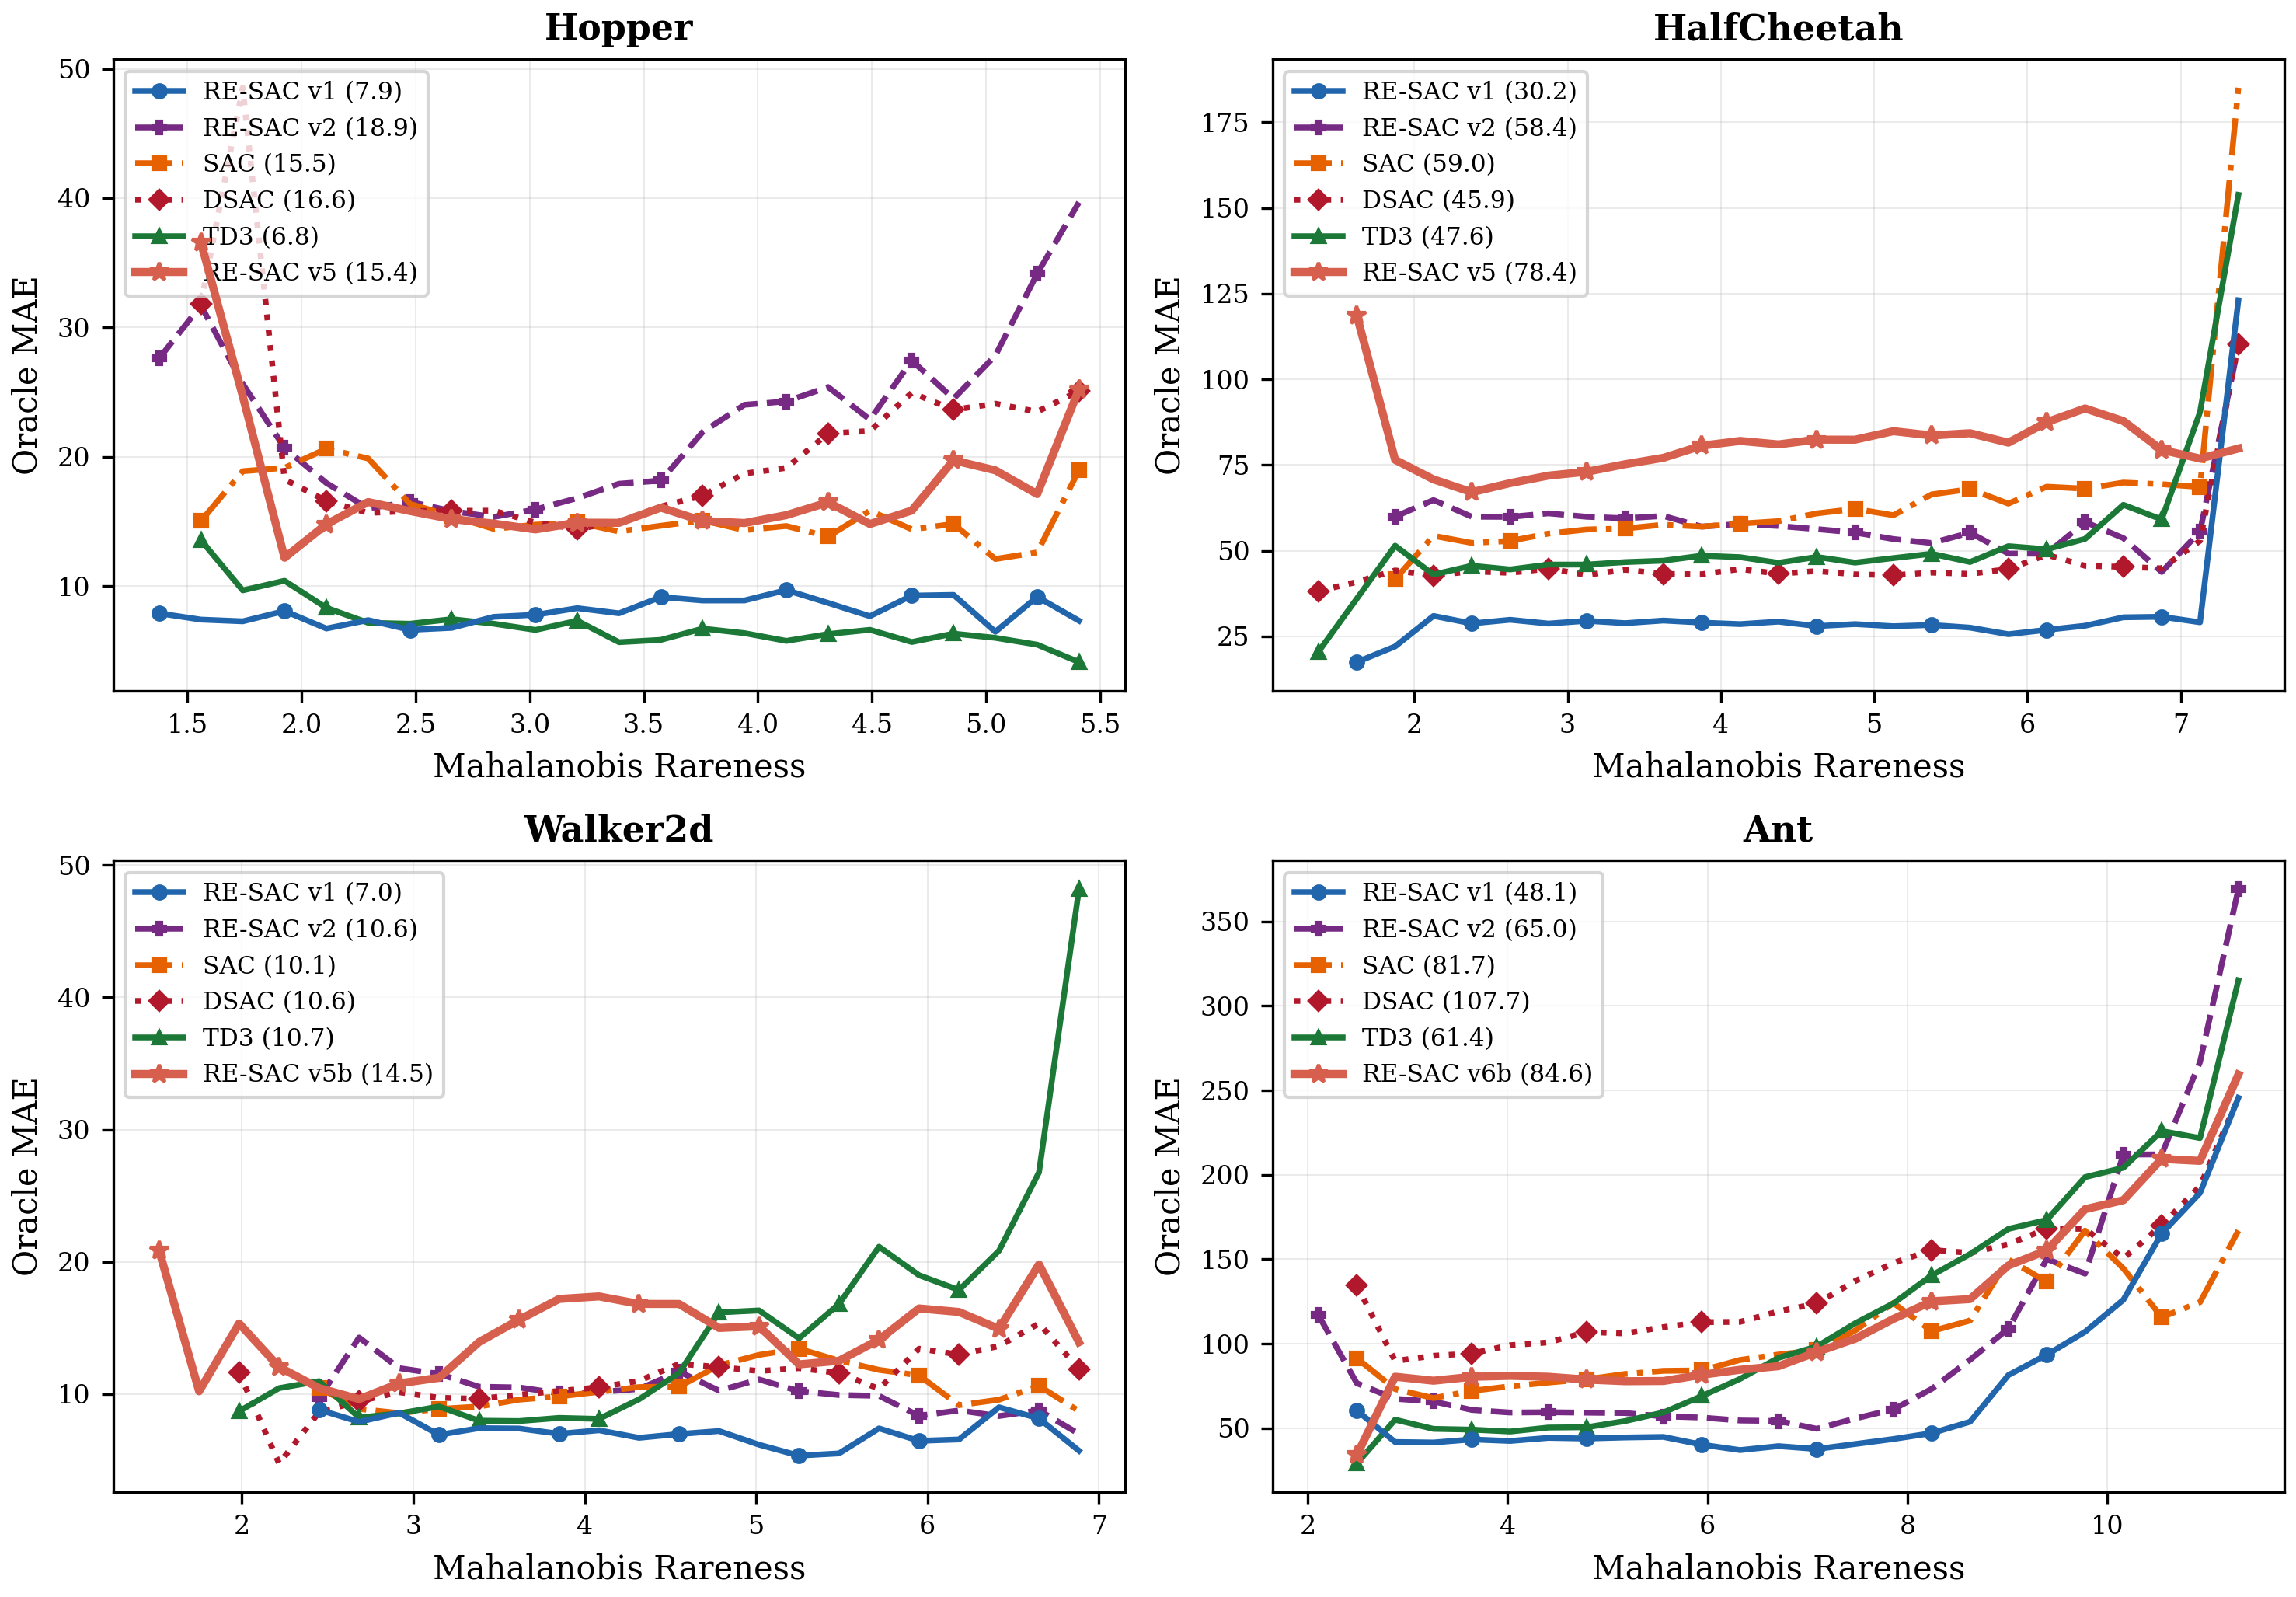
\includegraphics[width=\linewidth]{mujoco_oracle_q_error.png}
    \caption{Oracle Q-Error (MAE) binned by Mahalanobis rareness on four MuJoCo environments. Legend entries show overall Oracle MAE. RE-SAC v1 (solid blue) maintains the lowest estimation error in OOD regions; RE-SAC v5/v6b (red, starred) trades per-head accuracy for ensemble diversity that drives superior policy performance.}
    \label{fig:mujoco_oracle}
\end{figure}

\subsubsection{Training performance}
Fig.~\ref{fig:mujoco_curves} shows evaluation returns during training. RE-SAC v5 (thick red line, per-env best config) achieves the highest final return on all four environments: HalfCheetah 22711 (54\% above SAC), Walker2d 1008 (3.2$\times$ SAC, 2.2$\times$ DSAC), Hopper 660 (above SAC's 645), and Ant 27104 (v6b, surpassing DSAC's 25118). These gains stem from the independent target design preserving ensemble diversity: with meaningful Q-std, the adaptive $\beta_{lcb}$ schedule effectively balances exploration early (pessimistic $\beta{=}{-2}$) and exploitation later ($\beta \to -1$), while the EMA actor and policy anchor prevent the late-training instabilities observed in ablations without these mechanisms.

\begin{figure}[!htbp]
    \centering
    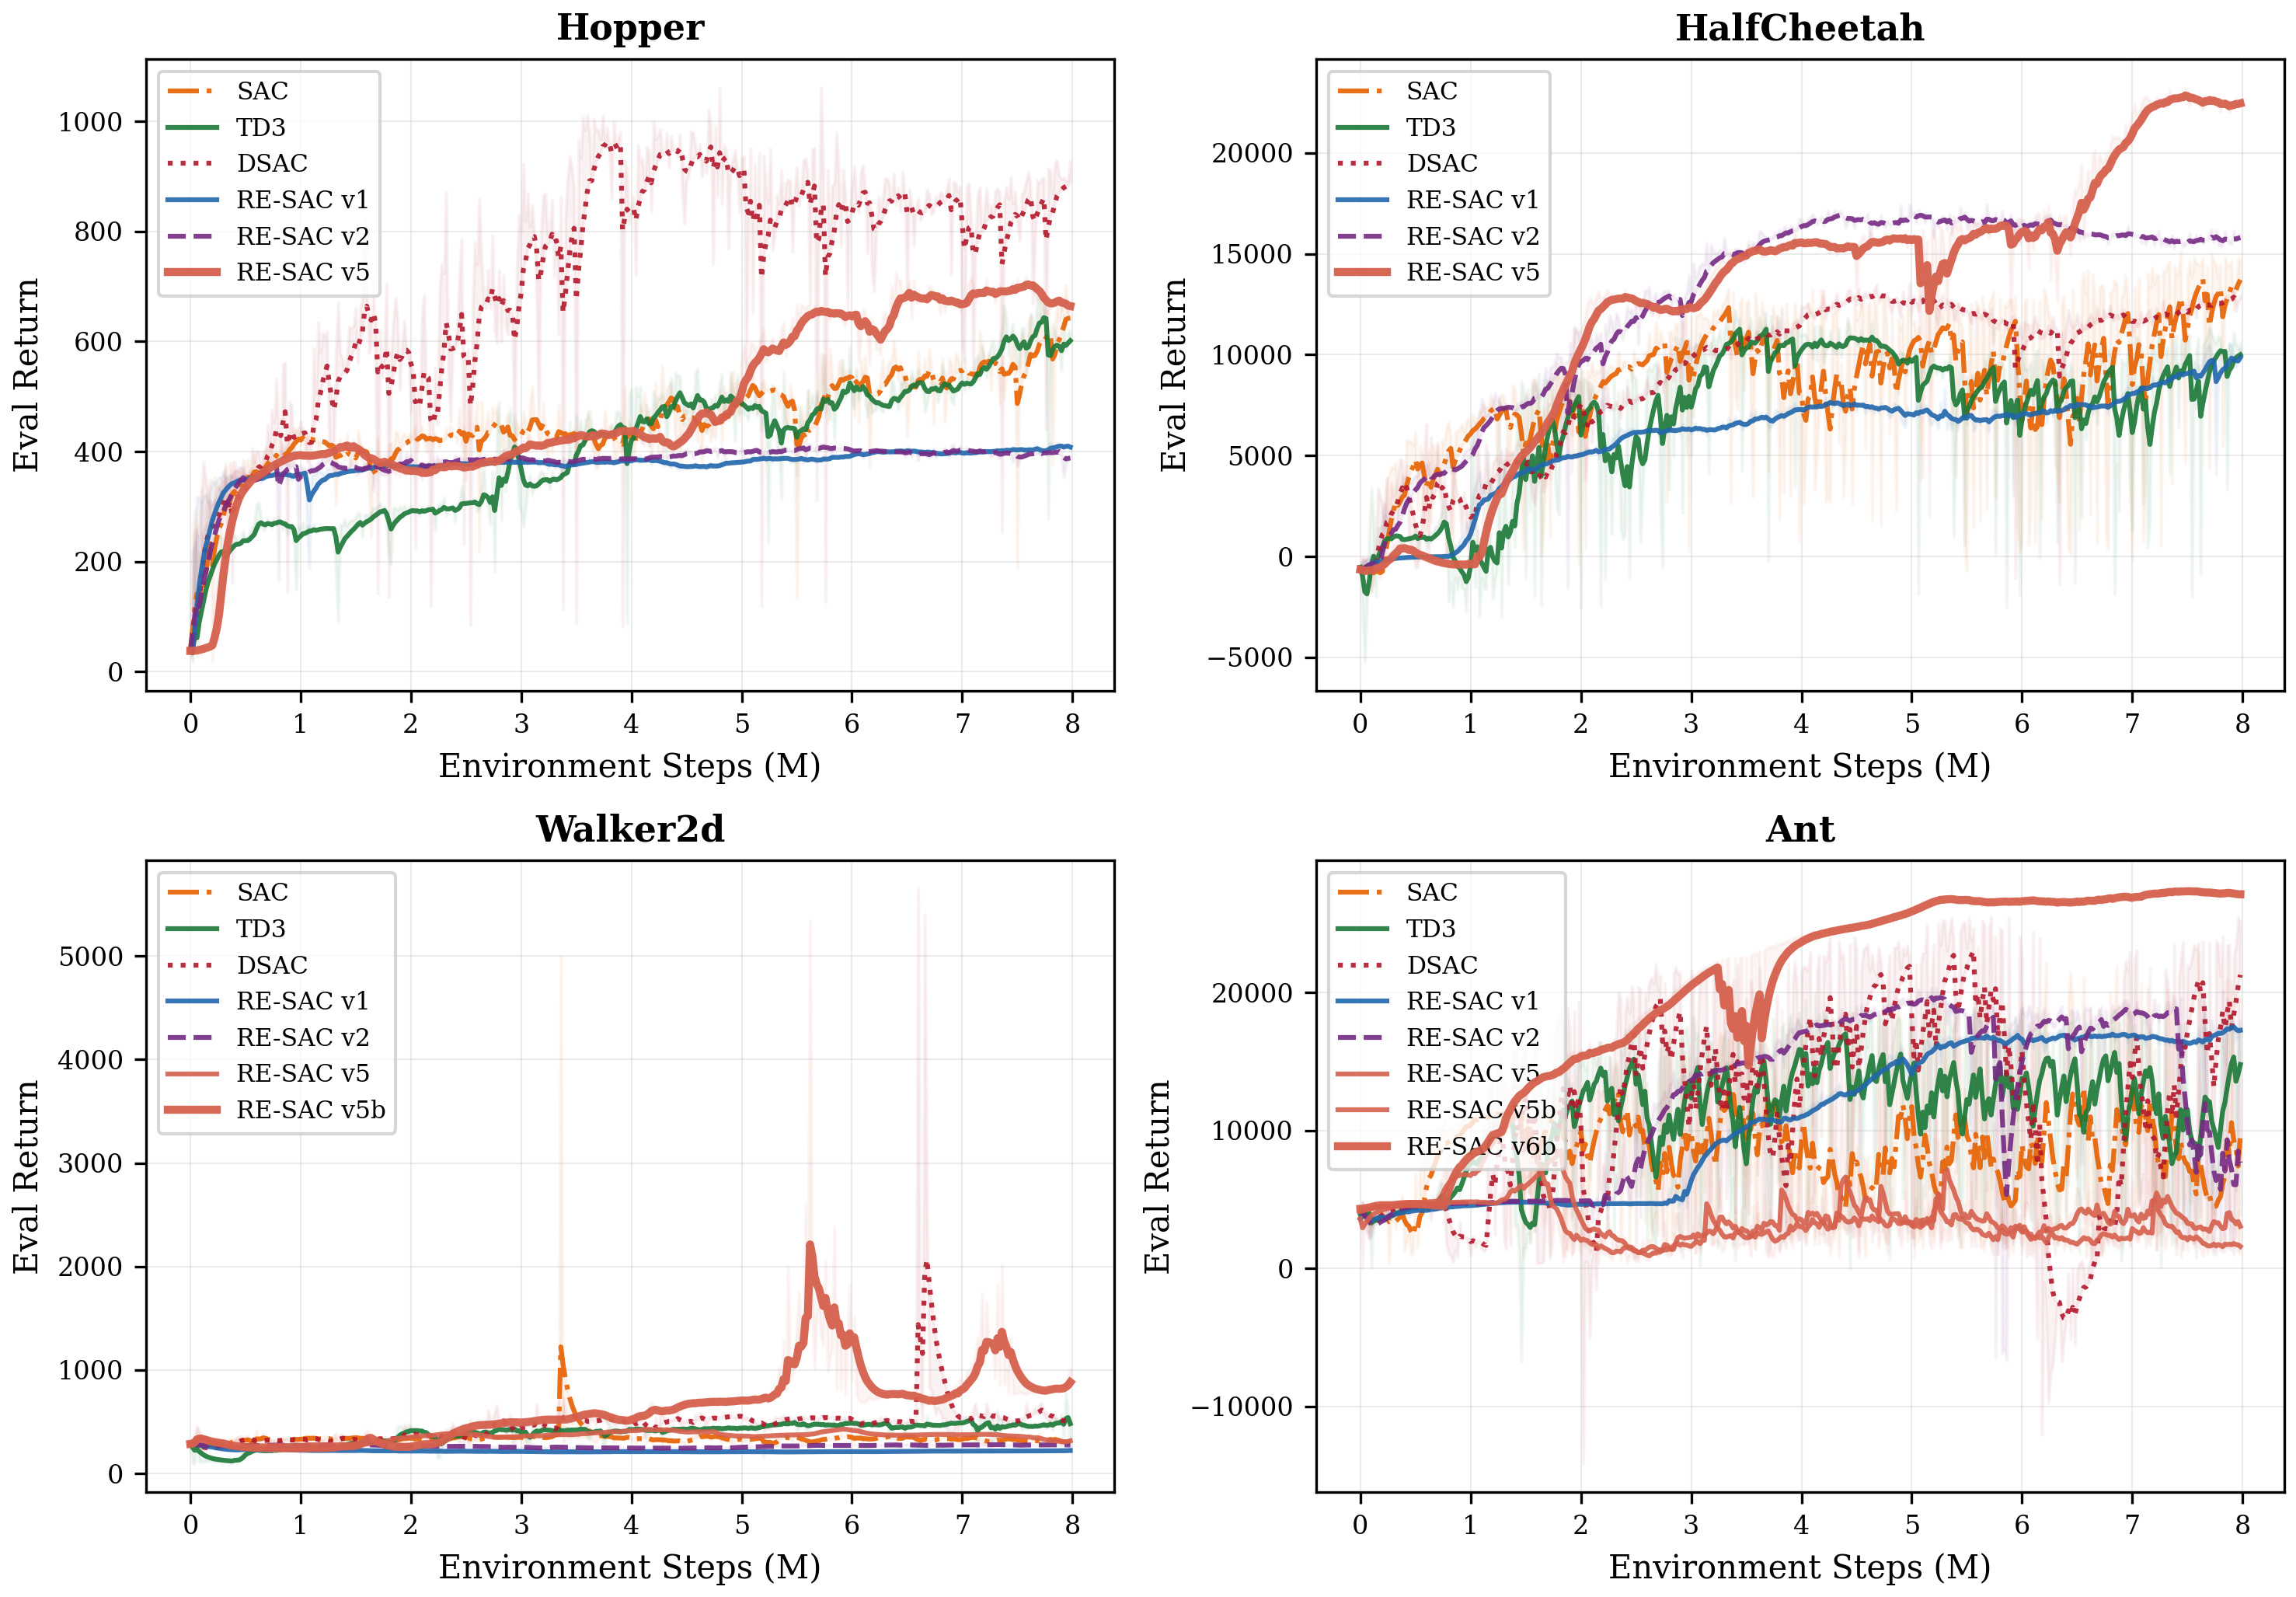
\includegraphics[width=\linewidth]{mujoco_training_curves.png}
    \caption{Evaluation returns on MuJoCo benchmarks (8M steps, seed 8). RE-SAC v5 (thick red) achieves the highest final return on all four environments by maintaining ensemble diversity through independent critic targets.}
    \label{fig:mujoco_curves}
\end{figure}

\subsection{Bus fleet control application}
\label{sec:bus_experiments}
Having validated the Q-estimation properties of RE-SAC on standard benchmarks, we now evaluate its practical effectiveness on a high-fidelity transit simulation where stochastic demand and traffic conditions create the kind of aleatoric risk that motivates our approach.

\subsubsection{Simulation environment}
We evaluate all algorithms on the bidirectional bus corridor simulation developed in our previous work~\cite{Zhang2025SingleAgentBus}. The environment models a realistic timetabled bus line with 22 stops (including two terminals) operating over a 13-hour service window (06:00--19:00). Buses are dispatched every 360 seconds from both terminals with a 180-second directional offset. Upon completing a trip, each vehicle becomes idle at its terminal and is available for reassignment according to the timetable, thereby modeling dynamic fleet sizing.

\textbf{Passenger demand} is specified by an hourly origin-destination (OD) matrix. For each pair of stations and each time period, passenger arrivals are sampled from a Poisson distribution with the corresponding time-varying rate. \textbf{Traffic conditions} are modeled as stochastic inter-stop travel speeds sampled from Gaussian distributions with hourly varying means and a fixed standard deviation of $\sigma = 1.5$~m/s, capturing realistic congestion fluctuations.

\textbf{MDP formulation.} The holding control problem is formulated as an event-driven MDP~\cite{Zhang2025SingleAgentBus}. Decisions are triggered after all passenger boarding/alighting activities have completed at each stop. The \textit{state} $s_t$ consists of categorical features (Bus~ID, Station~ID, Direction, Time~Period) and continuous features (forward headway $h_f$, backward headway $h_b$, current segment speed $v$). The \textit{action} $a_t \in [0, H_{max}]$ specifies the additional holding time at the current stop. The \textit{reward} follows the ridge-shaped function designed in~\cite{Zhang2025SingleAgentBus}, which simultaneously incentivizes headway regularity ($h_f \approx h_b \approx \tau$) and penalizes extreme deviations from the scheduled headway $\tau$.

\subsubsection{Network architecture and hyperparameters}
All algorithms are implemented in PyTorch. The $K$ critic networks are implemented as a single vectorized module (VectorizedCritic) for computational efficiency, each consisting of a 4-layer MLP with hidden dimensions $[64, 64, 64]$ and ReLU activations. The actor network is a separate 4-layer MLP with the same hidden dimension, outputting mean and log-standard-deviation for a squashed Gaussian policy. Following~\cite{Zhang2025SingleAgentBus}, categorical features (Bus~ID, Station~ID, Direction, Time~Period) are encoded via learnable embedding layers with dimension $d = \min(50, \lfloor N_i / 2 \rfloor)$, where $N_i$ is the number of unique categories. The embedded representations are concatenated with continuous state features (forward headway, backward headway, segment speed) to form the input vector.

Key hyperparameters are summarized as follows:
\begin{itemize}
    \item Ensemble size: $K \in \{2, 5, 10, 20, 40\}$ (default $K = 10$ unless otherwise specified);
    \item Learning rate: $1 \times 10^{-5}$ for critic, actor, and temperature (Adam optimizer);
    \item Batch size: 2048;
    \item Replay buffer size: $1 \times 10^6$ transitions;
    \item Discount factor: $\gamma = 0.99$;
    \item Target network smoothing coefficient: $\tau = 0.01$;
    \item Aleatoric regularization coefficient: $\lambda_{ale} = 0.01$ ($\ell_1$ weight penalty in critic target and loss; cf.\ Eq.~8);
    \item Actor LCB weight: $\beta_{lcb} = -2$ (applied as $\bar{Q} + \beta_{lcb} \cdot \sigma_{ens}$ in the actor objective; cf.\ Eq.~14);
    \item OOD penalty coefficient: $\beta_{ood} = 0.01$ (penalizes ensemble standard deviation in critic loss; cf.\ Eq.~12);
    \item Entropy temperature $\alpha$: automatically tuned via dual gradient descent with target entropy $\mathcal{H}_{target} = -\dim(\mathcal{A})$, capped at $\alpha_{\max} = 0.6$;
    \item Gradient clipping: max norm $= 1.0$;
    \item Critic-to-actor update ratio: $2:1$.
\end{itemize}
All baseline algorithms (SAC, DSAC, BAC) share the same network architecture, learning rate, and buffer configuration for fair comparison. Each experiment is trained for 500 episodes with training updates triggered every 5 environment steps, and evaluation metrics are averaged over 10 independent rollouts.

\subsubsection{Baselines and ablations}
To comprehensively evaluate our proposed method, we compare RE-SAC against state-of-the-art baselines and perform ablation studies to isolate the impact of our risk disentanglement.
\begin{itemize}
    \item \textbf{Vanilla SAC}~\cite{Haarnoja2018SAC}: The standard Soft Actor-Critic algorithm without explicit robust regularization or ensemble pessimism.
    \item \textbf{DSAC}~\cite{Ma2025DSAC}: Distributional Soft Actor-Critic, a risk-sensitive variant that learns the continuous return distribution to handle environmental stochasticity.
    \item \textbf{BAC}~\cite{Ji2024SeizingSerendipity}: BEE Actor-Critic~\cite{Ji2024SeizingSerendipity}, an off-policy actor-critic that exploits past successful experiences via the Blended Exploitation and Exploration (BEE) operator to avoid catastrophic value underestimation. We abbreviate it BAC (BEE Actor-Critic) throughout for brevity.
    \item \textbf{Epistemic only (ablation)}: A variant of RE-SAC that only applies the ensemble variance penalty $\Gamma_{epi}$, omitting the aleatoric weight regularization.
    \item \textbf{Aleatoric only (ablation)}: A variant that only applies the IPM-based weight regularization $\Gamma_{ale}$, omitting the ensemble.
\end{itemize}
For RE-SAC, we also evaluate the effect of the ensemble size $K \in \{2, 5, 10, 20, 40\}$.

\subsubsection{Overall performance and learning stability}
Fig.~\ref{fig:all_experiments} displays the smoothed cumulative rewards over training. Vanilla SAC and the Aleatoric-Only ablation suffer from suboptimal convergence, plateauing around a reward of $-0.55 \times 10^6$. The purely distributional baseline, DSAC-v1, performs slightly better but still falls short of the proposed method. Notably, the Epistemic-Only variant experiences a complete catastrophic collapse mid-training, dropping to $-1.2 \times 10^6$. This confirms our hypothesis: relying solely on ensemble variance in a highly stochastic environment misidentifies inherent noise as missing data, leading to runaway pessimism and policy degradation.

By successfully disentangling the uncertainties, RE-SAC (particularly with moderate ensemble sizes $K=5, 10, 20$) achieves the highest and most stable final reward (around $-0.4 \times 10^6$). Excessively large ensembles ($K=40$) show a slight performance degradation: with 40 parallel critics, the accumulated variance penalty $\lambda_{epi}\Gamma_{epi}$ becomes more sensitive to transient disagreements during early training, inducing a conservative bias that persists and slightly suppresses the final reward. This is consistent with the known over-pessimism of large ensembles in online settings~\cite{An2021UncertaintyEnsemble}. 
The BAC baseline, designed to avoid underestimation by exploiting past successes, performs relatively well but exhibits higher variance during training compared to RE-SAC, settling at a slightly lower final reward than the best RE-SAC variants. This suggests that while maintaining optimistic estimates of past serendipitous events helps avoid complete policy collapse in stochastic environments, explicitly disentangling and regularizing against aleatoric and epistemic risks provides a more stable and robust policy improvement path.

\begin{figure}[!htbp]
    \centering
    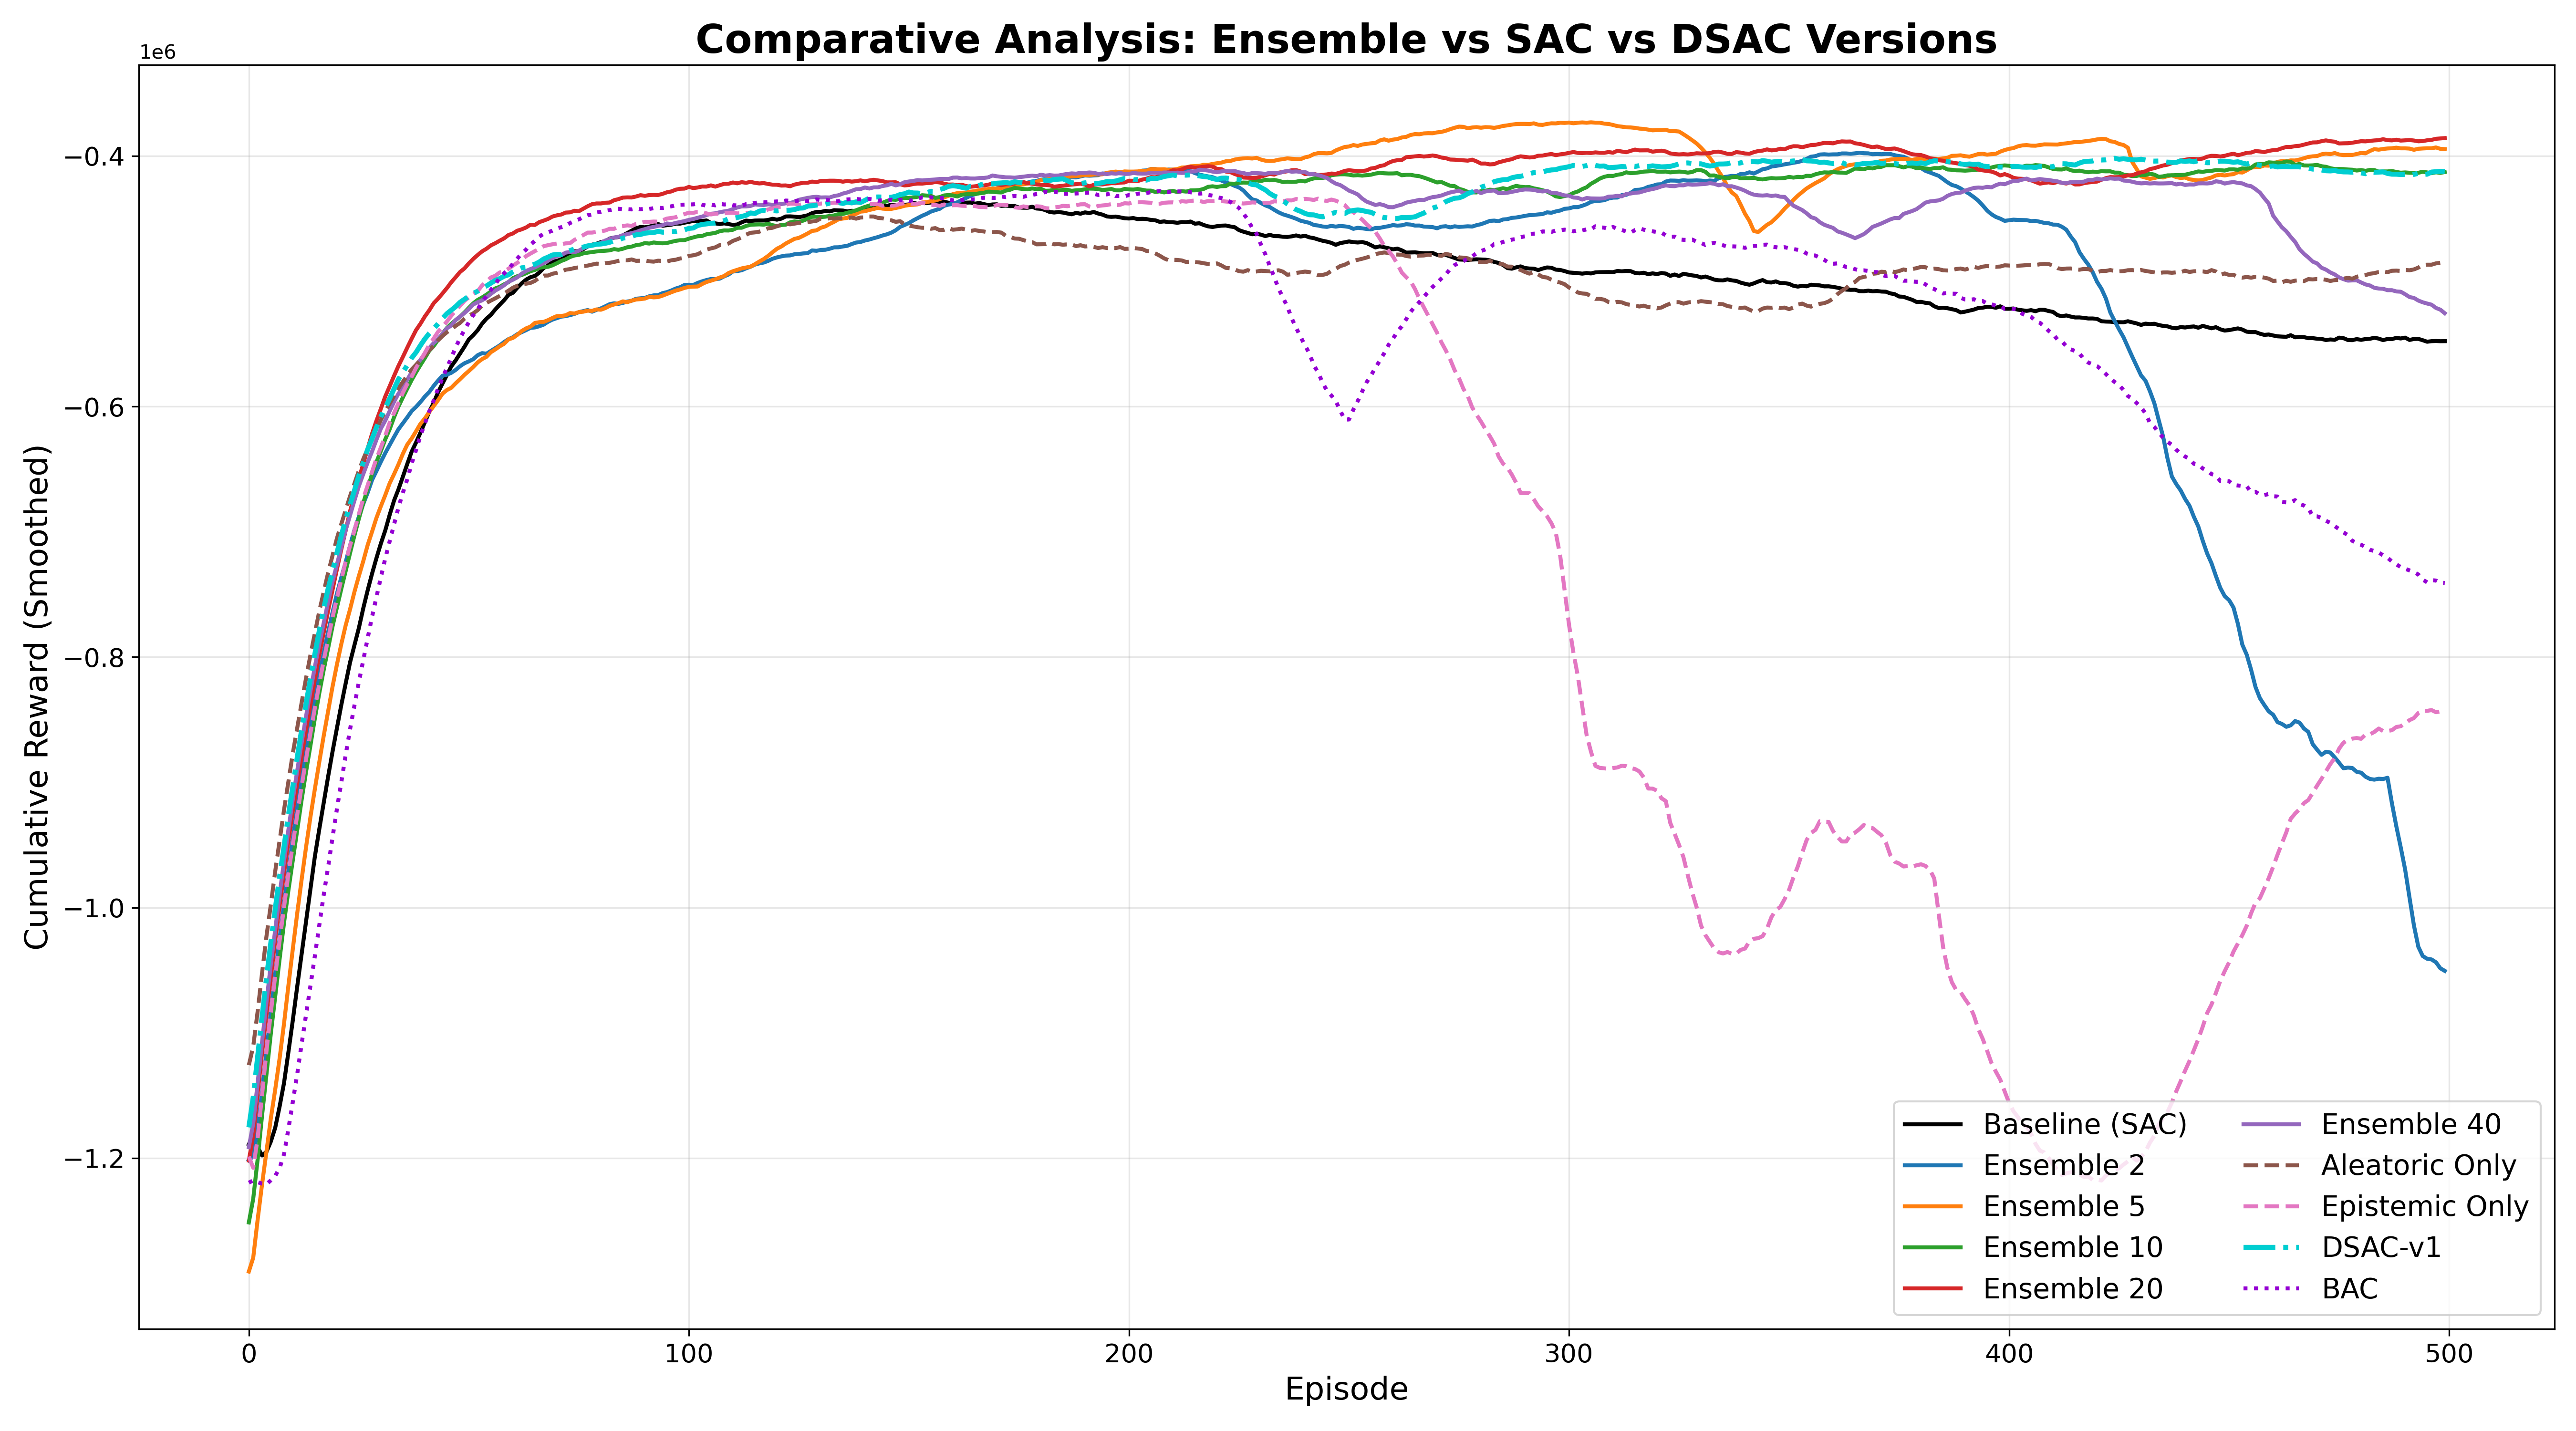
\includegraphics[width=\linewidth]{all_experiments_comparison_v2.png}
    \caption{Learning curves of cumulative reward for RE-SAC variants, SAC, DSAC-v1, BAC, and ablations.}
    \label{fig:all_experiments}
\end{figure}

\subsubsection{Q-value estimation stability}
The catastrophic drop in the Epistemic-Only policy is directly correlated with extreme value underestimation. As shown in Fig.~\ref{fig:all_q_values}, the estimated Q-values for the Epistemic-Only ablation plummet deep into negative values (passing $-3000$) with a massive $2\sigma$ variance band, corroborating the ``underestimation trap''. In contrast, RE-SAC variants and baseline SAC maintain relatively stable Q-value ranges. The disentangled penalties in RE-SAC prevent the variance penalty from overwhelming the nominal expected return.

\begin{figure}[!htbp]
    \centering
    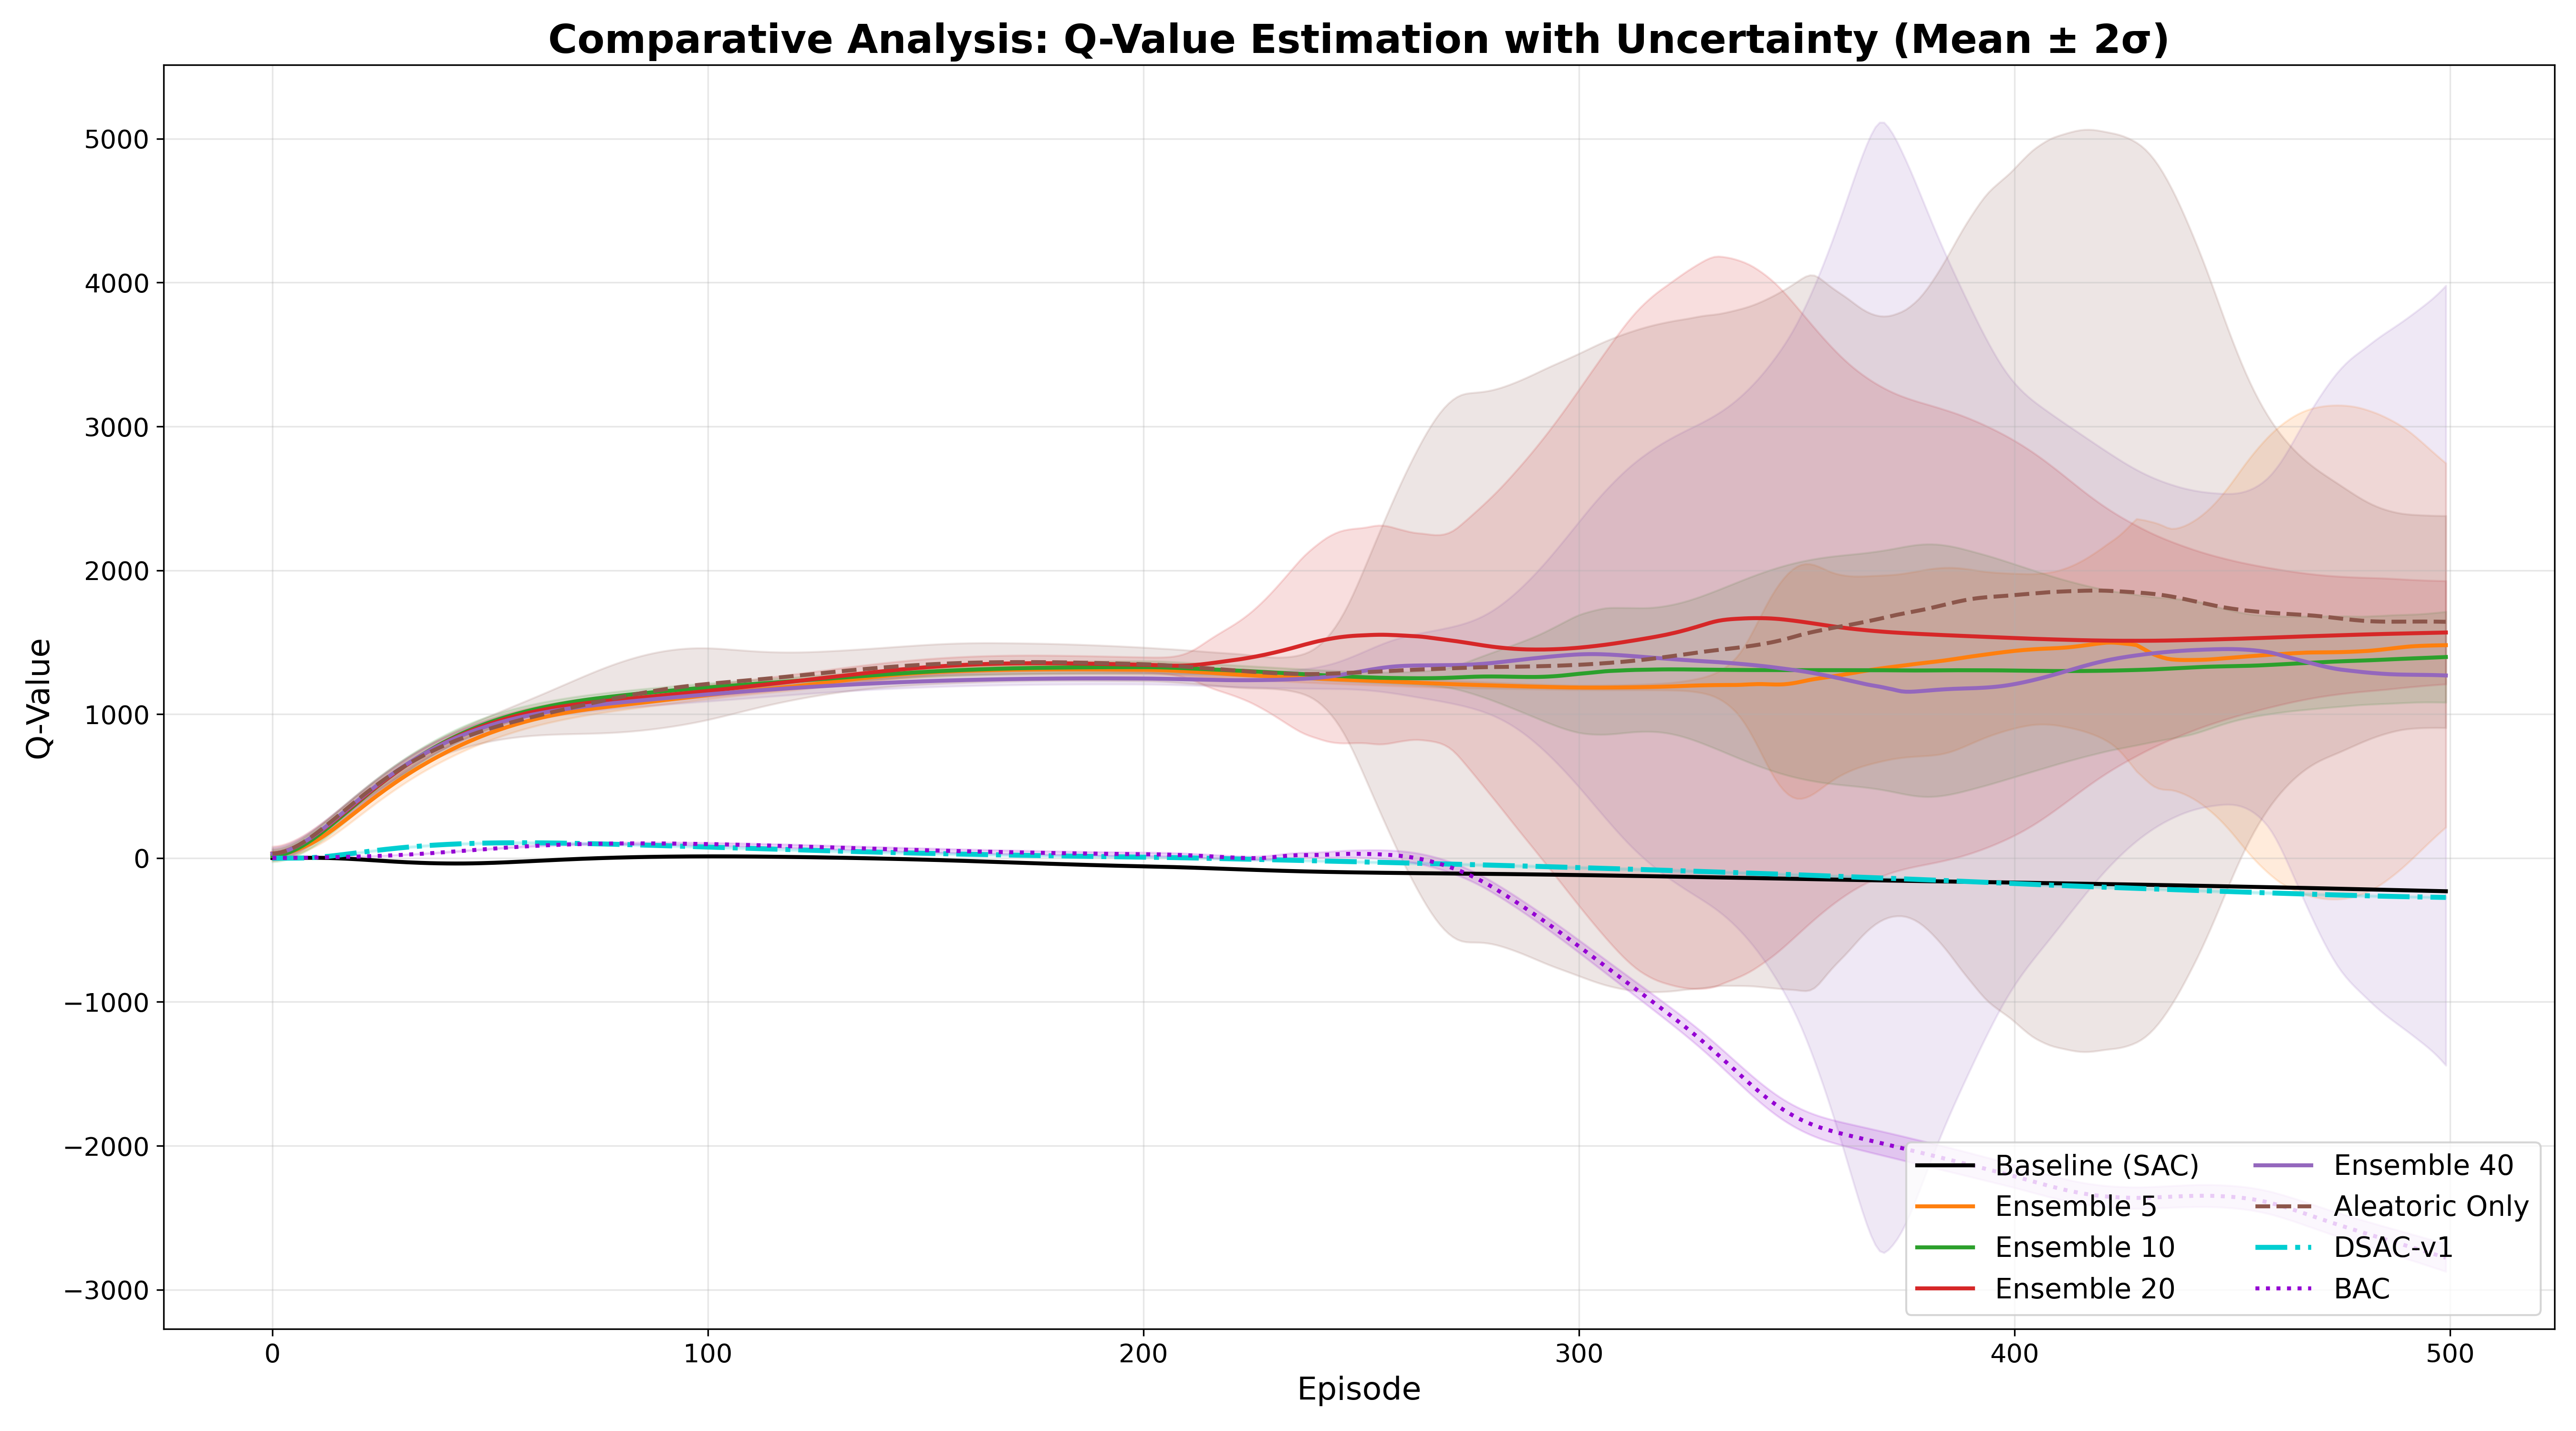
\includegraphics[width=\linewidth]{all_q_values_comparison_v2.png}
    \caption{Comparative analysis of estimated Q-Values (Mean $\pm$ $2\sigma$) over training.}
    \label{fig:all_q_values}
\end{figure}

\subsubsection{Robustness in rare states (Mahalanobis rareness)}
While the preceding Q-value analysis tracks estimation stability \emph{over training episodes}, a robust optimization perspective demands a complementary view: \emph{at the same level of state rarity, does the algorithm produce smaller estimation errors than baselines?} This distinction is essential because robust policies are valued not for their average-case accuracy, but for their ability to maintain bounded estimation errors in the worst-case regions of the state space.

To formalize this, we define \textbf{Mahalanobis rareness}. The key design choices are as follows. First, we condition on each \emph{spatial-directional group} (Station~ID $\times$ Direction), because different stops exhibit fundamentally different nominal headway distributions---for example, departure headways at terminals are tightly constrained by the timetable, whereas mid-route headways are subject to cumulative disturbances. A single global distribution would conflate structurally different operating regimes. For each group, we fit a 2D Gaussian to the observed continuous features (Forward Headway, Backward Headway), estimating the empirical mean $\mu$ and covariance $\Sigma$. Second, we use the \emph{Mahalanobis distance} rather than a simple Euclidean norm because the two headway features have different scales and are correlated (e.g., a very large forward headway typically co-occurs with a small backward headway in a bunching event). Euclidean distance is sensitive to these scale differences and ignores feature correlations, whereas the Mahalanobis distance $\sqrt{(x-\mu)^T\Sigma^{-1}(x-\mu)}$ naturally normalizes by the feature covariance, so that equally likely headway combinations receive equal rareness scores regardless of their direction in feature space. Intuitively, a state with high Mahalanobis rareness is one whose headway configuration the agent has rarely encountered at that stop during training---precisely the kind of state where epistemic risk is highest.

Fig.~\ref{fig:mahalanobis} bins the Mean Absolute Error (MAE) between each algorithm's Q-value estimates and the ground-truth Monte Carlo return $Q_{MC}(s,a)$ by Mahalanobis rareness. Here, $Q_{MC}$ is computed offline from the recorded evaluation trajectories as the discounted cumulative reward from each decision point onward: $Q_{MC}(s_t, a_t) = \sum_{k=0}^{T-t} \gamma^k r_{t+k}$, providing a model-free ground truth independent of any learned value function.

Since different algorithms learn Q-values at different absolute scales, direct comparison of raw prediction errors would be misleading. We therefore apply a per-algorithm z-score alignment that rescales each algorithm's predictions to match the mean and standard deviation of $Q_{MC}$ before computing the error. Additionally, for ensemble-based algorithms, we report the \textbf{Oracle MAE}: for each state, we select the ensemble head whose aligned prediction is closest to $Q_{MC}$, and compute the MAE over these best-head predictions. This oracle serves as a favorable upper bound on the ensemble's representational capacity---it measures how well the ensemble \textit{could} estimate the true return if paired with an ideal head-selection mechanism.

As states become increasingly rare (moving left to right on the x-axis), the estimation errors for Vanilla SAC and DSAC-v1 escalate significantly, confirming that their value networks extrapolate unreliably outside the training distribution. In contrast, RE-SAC (Ensemble) consistently demonstrates the lowest Oracle MAE across all rareness bins (overall average of 1647, compared to SAC's 4343 and DSAC's 5945). The tight error bands around the RE-SAC predictions confirm that the disentangled regularization structurally bounds the value network, preventing wild extrapolations in OOD regions and yielding superior worst-case guarantees.
\vspace{-2pt}
\begin{figure}[!htbp]
    \centering
    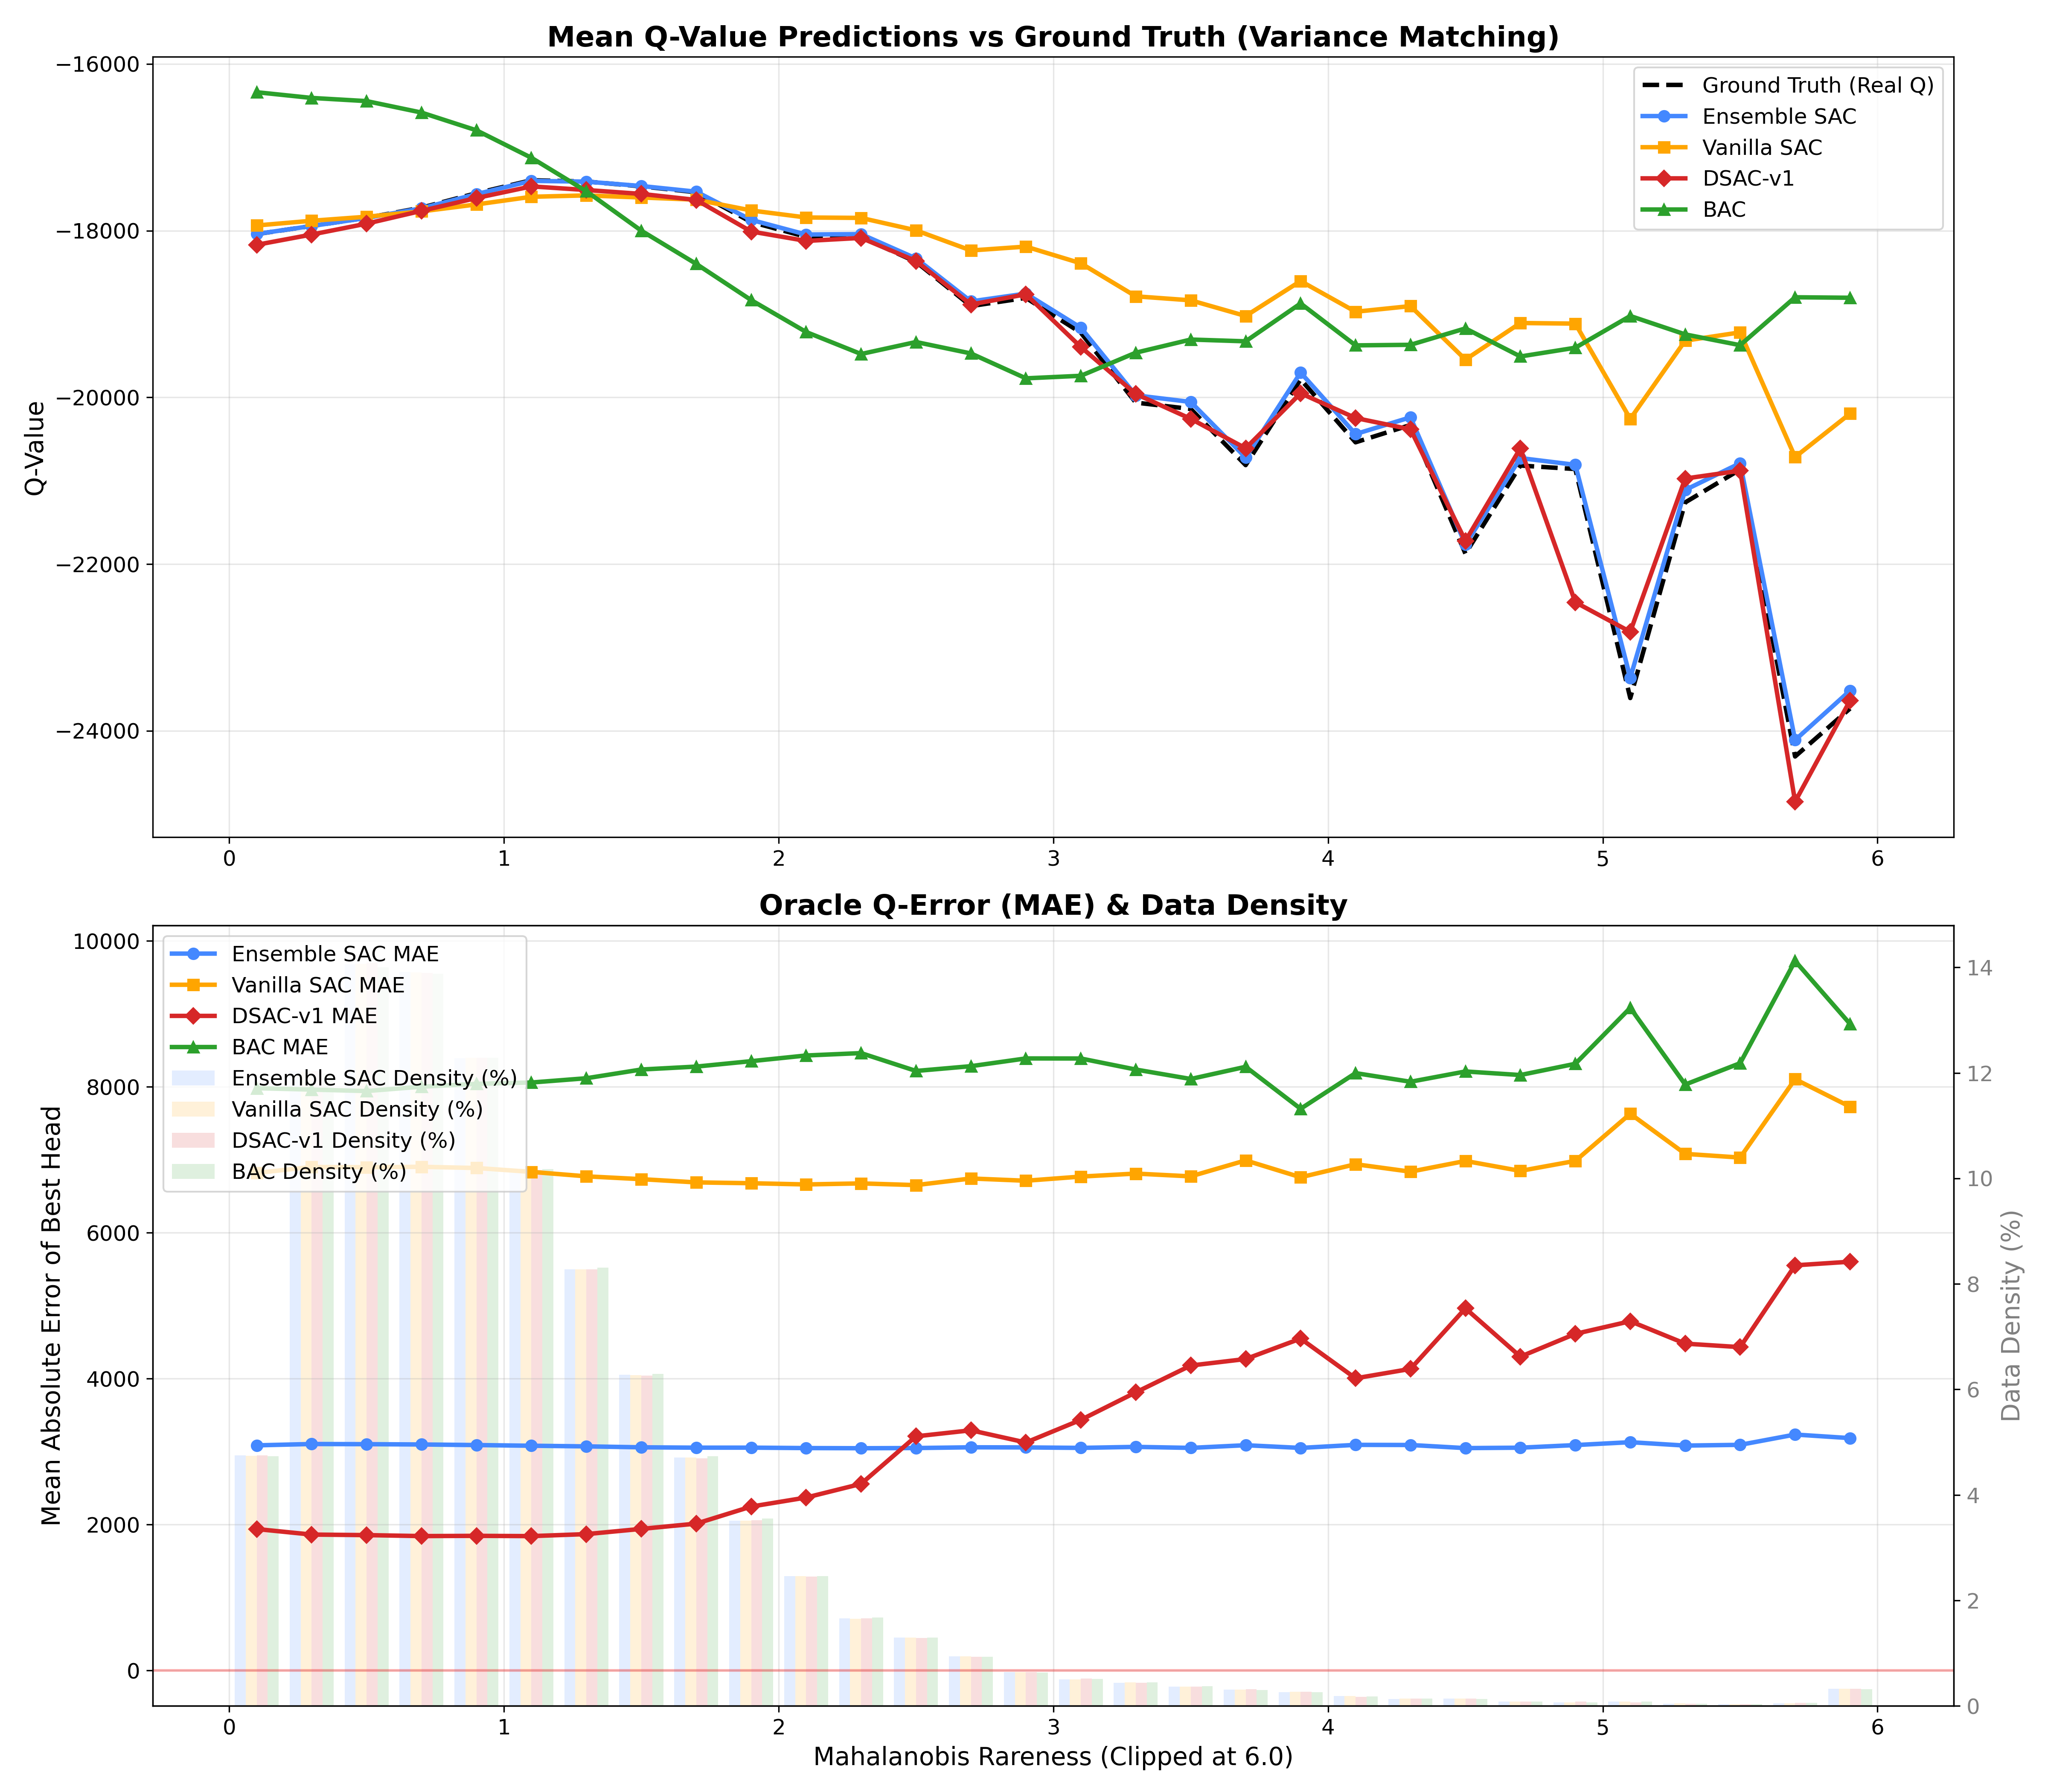
\includegraphics[width=\linewidth]{comparison_mahalanobis_rareness_restyled.png}
    \vspace{-6pt}
    \caption{Oracle Q-Error (MAE) banded by Mahalanobis Rareness. RE-SAC maintains accurate estimates even in highly rare/OOD states.}
    \label{fig:mahalanobis}
\end{figure}

\FloatBarrier
\section{Conclusion}
This paper presents the RE-SAC framework, a robust reinforcement learning approach that explicitly disentangles aleatoric and epistemic uncertainties. Grounded in the theoretical correspondence between risk-sensitivity and robustness established by Osogami~\cite{Osogami2012Robustness}, our method employs two complementary mechanisms: IPM-based weight regularization to enforce Lipschitz continuity of the value function against inherent environmental stochasticity, and a diversified $Q$-ensemble to penalize overconfident estimates in data-sparse regions of the state-action space.

Our theoretical analysis identifies a sharp structural boundary for contraction in multi-penalty Bellman operators: the frozen-parameter design (target networks for epistemic variance, held-fixed critic weights for aleatoric penalty) is both sufficient for $\gamma$-contraction and \emph{necessary}---Q-dependent penalties provably break it.  Both results are machine-verified in Lean~4 with no \texttt{sorry}, and a verifiable feasibility condition on the penalty coefficients guarantees policy non-degeneration (Appendix~\ref{app:nondegen}).  This structural insight---that the standard deep RL architecture of frozen target networks is not merely a stabilisation heuristic but a \emph{required} condition for operator contractiveness---may inform the design of future multi-penalty RL algorithms.

Empirically, on standard MuJoCo benchmarks, RE-SAC achieves the lowest Oracle Q-estimation error on 3 of 4 environments, reducing MAE by up to 55\% relative to DSAC and 41\% relative to SAC on the high-dimensional Ant task. On a realistic bidirectional bus simulation, RE-SAC achieves the highest and most stable cumulative reward among all baselines, including vanilla SAC, DSAC, and BAC. The ablation studies reveal that relying solely on ensemble variance (Epistemic-Only) leads to catastrophic value collapse in high-variance transit environments, while using only weight regularization (Aleatoric-Only) fails to detect out-of-distribution states. The Mahalanobis rareness analysis further confirms that RE-SAC maintains accurate $Q$-value estimates even under highly rare traffic states, exhibiting superior worst-case robustness.

In future work, we plan to extend this framework to multi-line transit networks with transfer coordination, investigate adaptive scheduling of the uncertainty coefficients $\lambda_{ale}$ and $\lambda_{epi}$ during training, and explore the integration of distributional RL methods with our disentangled robustness framework to further improve tail-risk management in urban transit systems.

\section*{Acknowledgments}
This work was supported by the National Natural Science Foundation of China (Grant No. 72371251), the Natural Science Foundation for Distinguished Young Scholars of Hunan Province (Grant No. 2024JJ2080), and the Key Research and Development Program of Hunan Province of China (Grant No. 2024JK2007).

\bibliographystyle{IEEEtran}
\documentclass[10pt]{article}
\usepackage[utf8]{inputenc}
\usepackage[T1]{fontenc}
\usepackage[margin=1in, left=1.25in, right=1.25in, top=1in, bottom=1in]{geometry}
\usepackage{algorithm}
\usepackage{algorithmic}
\usepackage[linktoc=all, bookmarksdepth=3, pdfstartview=FitH]{hyperref}
\hypersetup{colorlinks=true, linkcolor=blue, filecolor=magenta, urlcolor=cyan}
\urlstyle{same}
\usepackage{amsmath}
\usepackage{amsfonts}
\usepackage{amssymb}
\usepackage[version=4]{mhchem}
\usepackage{stmaryrd}
\usepackage{bbold}
\usepackage{graphicx}
\usepackage[export]{adjustbox}
\usepackage[dvipsnames]{xcolor}
\usepackage{float}
\usepackage{placeins}
\usepackage{caption}
\captionsetup[figure]{name=Fig.}
\usepackage{booktabs}
\usepackage{multirow}
% ==== Revision color macro (keep for marked version) ====
\usepackage[normalem]{ulem} % for \sout
\usepackage{amsthm}
\usepackage{enumitem}
\newtheorem{theorem}{Theorem}[section]
\newtheorem{lemma}[theorem]{Lemma}
\newtheorem{definition}[theorem]{Definition}
\newtheorem{corollary}[theorem]{Corollary}
\newtheorem{proposition}[theorem]{Proposition}
\newtheorem{remark}[theorem]{Remark}
% \newcommand{\revise}[1]{{\color{blue}#1}}
% \newcommand{\del}[1]{\color{red}{\sout{#1}}}             % deletions (red strikeout)
\newcommand{\revise}[1]{#1}
\newcommand{\del}[1]{}

% ==== Algorithm package ====
% Option A: algorithm2e
% \usepackage[ruled,vlined,linesnumbered]{algorithm2e}
% Or Option B: algpseudocode


\graphicspath{ {./} }

\title{RE-SAC: Disentangling aleatoric and epistemic risks in bus fleet control: A stable and robust ensemble DRL approach\footnote{Code available at \url{https://github.com/erzhu419/RE-SAC}}}

\author{
  Yifan Zhang\thanks{Central South University, \href{mailto:erzhu419@gmail.com}{erzhu419@gmail.com}, \href{mailto:204201048@csu.edu.cn}{204201048@csu.edu.cn}} \and
  Liang Zheng\thanks{Central South University, \href{mailto:zhengliang@csu.edu.cn}{zhengliang@csu.edu.cn}}
}
\date{}


%New command to display footnote whose markers will always be hidden
\let\svthefootnote\thefootnote
\newcommand\blfootnotetext[1]{%
  \let\thefootnote\relax\footnote{#1}%
  \addtocounter{footnote}{-1}%
  \let\thefootnote\svthefootnote%
}

%Overriding the \footnotetext command to hide the marker if its value is `0`
\let\svfootnotetext\footnotetext
\renewcommand\footnotetext[2][?]{%
  \if\relax#1\relax%
    \ifnum\value{footnote}=0\blfootnotetext{#2}\else\svfootnotetext{#2}\fi%
  \else%
    \if?#1\ifnum\value{footnote}=0\blfootnotetext{#2}\else\svfootnotetext{#2}\fi%
    \else\svfootnotetext[#1]{#2}\fi%
  \fi
}

\begin{document}
\maketitle


\begin{abstract}
Bus holding control remains a persistent challenge in urban transit systems due to the inherent stochasticity of traffic conditions and passenger demand. While deep reinforcement learning (DRL) has shown promise for dynamic holding decisions, standard actor-critic algorithms frequently suffer from $Q$-value instability in highly volatile environments. A key yet underexplored source of this instability is the conflation of two structurally distinct uncertainties: \textit{aleatoric} uncertainty, arising from irreducible environmental noise, and \textit{epistemic} uncertainty, arising from data insufficiency in the replay buffer. Treating these as a single risk leads to pathological underestimation in well-explored but noisy states, ultimately causing catastrophic value collapse.

In this paper, we propose a robust ensemble soft actor-critic (RE-SAC) framework that explicitly disentangles and addresses both sources of uncertainty. Our approach applies Integral Probability Metric (IPM)-based weight regularization to the critic network to hedge against aleatoric risk, providing a smooth analytical lower bound for the robust Bellman operator without requiring expensive inner-loop state perturbations. To address epistemic risk, a diversified $Q$-ensemble penalizes overconfident value estimates in sparsely covered regions of the state-action space. This dual mechanism prevents the ensemble variance from misidentifying inherent noise as a data gap, a failure mode that causes complete policy collapse in our ablation study.

Empirically, experiments in a realistic bidirectional bus corridor simulation demonstrate that RE-SAC achieves the highest and most stable cumulative reward (approximately $-0.4 \times 10^6$) among all baselines, compared to $-0.55 \times 10^6$ for vanilla SAC and $-1.2 \times 10^6$ for the epistemic-only ablation. The Mahalanobis rareness analysis further confirms that RE-SAC reduces \emph{Oracle} Q-value estimation error by up to $62\%$ in rare out-of-distribution states relative to SAC (average Oracle MAE of 1647 vs.\ 4343), demonstrating superior worst-case robustness under high traffic variability.
Our theoretical analysis further reveals that the frozen-parameter design (target networks, held-fixed critic weights) is not merely a practical stabilisation heuristic but a \emph{structurally necessary condition} for Bellman operator contractiveness under multi-penalty regularisation---an insight with implications beyond transit control.
\end{abstract}


\noindent\textbf{Keywords:} bus bunching; robust reinforcement learning; ensemble; uncertainty decomposition; bus holding control.


\section{Introduction}

Bus bunching---the phenomenon where multiple buses on the same route cluster together---remains a well-known challenge in urban transit systems. This instability is driven by a positive feedback loop: a slight delay at a stop increases passenger accumulation, which extends dwell time, further slowing the leading bus while the trailing bus speeds up due to reduced demand~\cite{Daganzo2009Headway, Xuan2011Dynamic}. To break this cycle, various holding control strategies have been developed, transitioning from classical schedule-based optimization to deep reinforcement learning (DRL) paradigms~\cite{Wang2020DynamicHolding}.
However, despite the promising performance of DRL in controlled simulations, these models often exhibit fragile behavior when deployed in realistic, high-variance transit environments.

A critical, yet frequently overlooked bottleneck in applying Actor-Critic methods to transit control is what we term ``$Q$-value poisoning.'' In public transportation, stochasticity is not a transient disturbance but a deeply ingrained feature; fluctuations in passenger arrival rates and road traffic speeds are often irreducible. In such highly volatile environments, standard off-policy algorithms like Soft Actor-Critic (SAC) frequently suffer from pathological value estimation degradation. As training progresses, the $Q$-function may become ``poisoned'' by environmental noise, leading to severe underestimation of successful past interventions or wild oscillations in unvisited state-action regions. This phenomenon, consistent with the ``value collapse'' identified by recent studies~\cite{Ji2024SeizingSerendipity}, effectively paralyzes the agent's policy, causing it to fall into an under-exploitation trap where it fails to maintain regularity despite having encountered optimal trajectories in its experience buffer.

\begin{definition}[$Q$-value Poisoning]
    \label{def:poisoning}
    Let $Q^*$ be the optimal $Q$-function and $Q_t$ be the learned $Q$-function after $t$ gradient steps.
    Let $\sigma^2(s,a) := \mathrm{Var}_{P}[V_t(s') \mid s,a]$ denote the local aleatoric variance at $(s,a)$.
    We say the learning process suffers from \emph{$Q$-value poisoning} if there exist
    a threshold $\sigma^2_0 > 0$ and a non-vanishing set of state-action pairs
    $\mathcal{P}_t \subseteq \mathcal{S}\times\mathcal{A}$ such that:
    \begin{enumerate}[label=(\roman*)]
        \item \textbf{Selective underestimation in high-variance regions:}
        $Q_t(s,a) < Q^*(s,a)$ for all $(s,a)\in\mathcal{P}_t$ with
        $\sigma^2(s,a) \ge \sigma^2_0$; and
        \item \textbf{Accurate estimation in low-variance regions:}
        $|Q_t(s,a) - Q^*(s,a)| \le \epsilon$ for $(s,a)\notin\mathcal{P}_t$
        with $\sigma^2(s,a) < \sigma^2_0$.
    \end{enumerate}
    This pattern---accurate in low-noise states, poisoned in high-noise states---is
    \emph{structurally distinct} from classical overestimation bias
    ($Q_t \ge Q^*$ uniformly) and from the Deadly Triad
    (divergence of $\|Q_t\|_\infty \to \infty$); see Appendix~\ref{app:poisoning_vs_classical}.
\end{definition}

We argue that this instability is deeply rooted in the entanglement of dual uncertainties within the transit system. Following the taxonomy established by Depeweg et al.~\cite{Depeweg2018Decomposition} and Clements et al.~\cite{Clements2019EstimatingRisk}, we categorize these risks as:
\begin{enumerate}
    \item \textbf{Aleatoric Uncertainty:} The inherent and irreducible randomness of the traffic system, such as stochastic signal timings and bursty passenger surges at stations~\cite{Hullermeier2021AleatoricEpistemic}.
    \item \textbf{Epistemic Uncertainty:} The lack of model knowledge in regions of the state-action space poorly covered by the experience buffer, often exacerbated by the data imbalance inherent in offline or long-tail transit scenarios~\cite{An2021UncertaintyEnsemble}.
\end{enumerate}
In vanilla DRL, these two risks are conflated~\cite{Kendall2017WhatUncertainties}. An agent might over-penalize a state due to inherent aleatoric noise or show dangerous optimism in epistemic-deficient regions due to function approximation errors~\cite{Fujimoto2018TD3}.

To mitigate $Q$-value poisoning, a theoretically rigorous approach is to model the uncertainty distribution using Bayesian methods~\cite{Derman2019BayesianRobust, Depeweg2018Decomposition}. However, maintaining full posterior beliefs (e.g., Dirichlet distributions) for every state-action pair is intractable in high-dimensional continuous control. To circumvent this, we pivot to the framework of Robust Markov Decision Process (MDP)~\cite{Wiesemann2013RobustMDP}, which seeks a policy optimal against a worst-case uncertainty set. Building on the insights of Osogami~\cite{Osogami2012Robustness} and Xu et al.~\cite{Xu2009RobustLasso, Xu2009RobustSVM}, we treat this robust objective as mathematically equivalent to regularization in function space. This allows us to hedge against aleatoric risk by introducing an IPM-based network weight regularization term~\cite{Zhou2023NaturalActorCritic, Panaganti2024RobustF}, acting as a structural prior to suppress aleatoric-induced oscillations~\cite{Asadi2018Lipschitz}. Yet, regularization alone is a uniform prior; it cannot detect the ``unknown unknowns.'' Therefore, for epistemic risk, we complement this with a diversified $Q$-ensemble~\cite{An2021UncertaintyEnsemble, Osband2016BootstrappedDQN} to penalize data insufficiency.

Building upon our previous work on single-agent robust control for bus fleets~\cite{Zhang2025SingleAgentBus}, this paper introduces the RE-SAC framework.
More broadly, our results suggest that \emph{contraction in regularised reinforcement learning is not a generic property of penalised Bellman operators}, but depends critically on whether the penalty term is fixed or value-function-dependent during each backup step.
Making this structural assumption explicit---and verifying it formally---is essential for a correct theoretical understanding of modern deep RL algorithms.
Our contributions are summarized as follows:
\begin{itemize}
    \item \textbf{Theoretical disentanglement:} We provide a formal motivation for decoupling aleatoric and epistemic risks in transit control, bridging the gap between risk-sensitive RL~\cite{Osogami2012Robustness} and bus service reliability.
    \item \textbf{Structural stability characterisation:} We identify a sharp boundary for contraction in multi-penalty Bellman operators: penalties that are \emph{fixed} per backup step (frozen critic weights, target networks) preserve $\gamma$-contraction, while Q-dependent penalties provably break it.  Both the positive and negative results are machine-verified in Lean~4 with no \texttt{sorry} (\texttt{RESAC.lean}, \texttt{RESAC-Counterproof.lean}).  This reveals a \emph{necessary design condition} for stability in regularised RL---the frozen-parameter architecture used in practice (DQN, SAC, TD3) is not merely convenient but structurally required.
    \item \textbf{Analytic robustness:} We incorporate an IPM-based weight regularization~\cite{Zhou2023NaturalActorCritic} as a computationally efficient alternative to conservative smoothing~\cite{Yang2022RORL}, preventing $Q$-value collapse in stochastic environments.
    \item \textbf{Empirical stability:} Through extensive simulations in bidirectional corridors, we demonstrate that our approach prevents the underestimation pitfall~\cite{Ji2024SeizingSerendipity} and maintains superior service regularity compared to baseline algorithms including SAC, DSAC, and BAC.
\end{itemize}

\section{Related work}

\subsection{Bus fleet control and reinforcement learning}
Bus holding control has transitioned from classical theoretical models---such as headway-based exponential models~\cite{Daganzo2009Headway} and linear control for schedule reliability~\cite{Xuan2013BusHolding}---to data-driven optimization strategies. In recent years, DRL has emerged as a powerful tool for dynamic holding decisions~\cite{Wang2020DynamicHolding}. While many studies explore Multi-Agent Reinforcement Learning (MARL) to handle the coupling between vehicles, these systems often struggle with non-stationarity and the high computational cost of coordination~\cite{Gronauer2022MultiAgent, Papoudakis2019NonStationarity, Vinyals2019StarCraft}. Building upon our previous work, which demonstrated that a single-agent architecture can achieve robust bus fleet control through categorical embeddings~\cite{Zhang2025SingleAgentBus}, this study focuses on the fundamental stability of value estimation in such stochastic environments.

\subsection{Uncertainty quantification in RL: from Bayesian and risk-sensitive to robust methods}
The handling of uncertainty in RL has evolved through two main lineages: Bayesian distributional modeling and risk-sensitive optimization. Bayesian approaches~\cite{Depeweg2018Decomposition, Derman2019BayesianRobust} theoretically resolve epistemic uncertainty by maintaining posteriors over system dynamics. Parallel to this, risk-sensitive RL optimizes tail risk measures like Conditional Value at Risk (CVaR)~\cite{Chow2014CVaR, Chow2015RiskSensitive}, a line of work further advanced by distributional RL~\cite{Bellemare2017Distributional, Dabney2018QuantileRegression}. However, both paradigms face significant hurdles: Bayesian methods struggle with the intractability of posterior updates in high dimensions, while direct risk optimization often incurs prohibitive sampling complexity, as Fei et al.~\cite{Fei2020RiskSensitive} demonstrated that risk-sensitive regret bounds scale significantly worse than standard RL (see Appendix~\ref{app:complexity}). To circumvent these barriers, the field has turned to Robust Markov Decision Processes (RMDPs)~\cite{Wiesemann2013RobustMDP, Iyengar2005RobustDP}, where uncertainty is enclosed within a static set. The unification of these views came when Osogami~\cite{Osogami2012Robustness} linked robust objectives to risk-sensitive MDPs, bridging worst-case optimization and risk aversion. Complementing this, Geist et al.~\cite{Geist2019TheoryRegularized} showed a key insight: regularization in MDPs effectively imposes a \textit{prior distribution} on the policy or value function, so that a regularized update can be interpreted as a quasi-Bayesian posterior estimation (see Appendix~\ref{app:regularization_prior}). This justifies network regularization as a scalable proxy for handling inherent system stochasticity (aleatoric risk).

\subsection{Disentangling aleatoric and epistemic risks}
Relying solely on regularization acts as a uniform prior, effectively smoothing the policy against aleatoric noise but failing to identify regions of data insufficiency (Epistemic Risk). To address this, we adopt the decomposition framework of Clements et al.~\cite{Clements2019EstimatingRisk} and Depeweg et al.~\cite{Depeweg2018Decomposition}. We employ a diversified $Q$-ensemble~\cite{An2021UncertaintyEnsemble, Osband2016BootstrappedDQN} to quantify epistemic uncertainty through predictive variance, penalizing over-optimism in sparsely sampled regions. Simultaneously, we use IPM-based weight regularization~\cite{Zhou2023NaturalActorCritic} to enforce local Lipschitz continuity~\cite{Asadi2018Lipschitz}, providing a tight lower bound against aleatoric perturbations. This dual approach leverages the efficiency of regularization for aleatoric risk and the sensitivity of ensembles for epistemic risk, preventing the value collapse typically observed in high-variance transit environments~\cite{Ji2024SeizingSerendipity}.

\subsection{Stability and the underestimation trap}
Function approximation errors are a well-known source of instability in Actor-Critic methods, typically leading to overestimation bias~\cite{VanHasselt2010DoubleQ, Fujimoto2018TD3}. While SAC utilizes maximum entropy to improve exploration~\cite{Haarnoja2018SAC}, it remains vulnerable to ``value collapse'' when local batches fail to represent the true high-variance distribution. Recent broad studies suggest that excessive pessimism---often used in offline RL~\cite{Yang2022RORL, Kumar2020CQL}---can lead to an ``underestimation trap'' in online settings where the agent ignores high-value trajectories~\cite{Ji2024SeizingSerendipity}. Our work synthesizes these insights to maintain value estimation stability without succumbing to the pathological degradation often seen in vanilla robust implementations.

\section{Preliminaries}

\subsection{Maximum entropy MDP}
We formulate the bus holding problem as an MDP, characterized by the tuple $(\mathcal{S}, \mathcal{A}, P, R, \gamma)$. In the Maximum Entropy Reinforcement Learning framework~\cite{Haarnoja2018SAC}, the agent's objective is to jointly maximize the expected cumulative return and the policy's entropy. This objective is formally expressed as:
\begin{equation}
    J(\pi) = \mathbb{E}_{\pi, P} \left[ \sum_{t=0}^{\infty} \gamma^t \left( R(s_t, a_t) + \alpha \mathcal{H}(\pi(\cdot|s_t)) \right) \right],
\end{equation}
where $\mathcal{H}(\pi(\cdot|s_t))$ denotes the Shannon entropy of the policy, and $\alpha$ is the temperature parameter controlling the exploration-exploitation trade-off. The corresponding soft state value function $V^\pi(s)$ and soft action-value function $Q^\pi(s, a)$ are related by:
\begin{equation}
    V^\pi(s) = \mathbb{E}_{a \sim \pi} [Q^\pi(s, a) - \alpha \log \pi(a|s)].
\end{equation}
The Soft Bellman Operator $\mathcal{T}^\pi$ acts on $Q$-functions as $\mathcal{T}^\pi Q(s, a) = R(s, a) + \gamma \mathbb{E}_{s' \sim P} [V^\pi(s')]$, forming a contraction mapping that guarantees convergence to the optimal soft $Q$-function.

\subsection{Robust Markov decision process}
A Robust MDP (RMDP) generalizes the standard MDP by replacing the fixed transition kernel $P$ with an uncertain set of transition probabilities $\mathcal{P}_{s,a}$ for each state-action pair $(s,a)$~\cite{Iyengar2005RobustDP, Wiesemann2013RobustMDP}. The agent seeks a policy that maximizes the worst-case expected return over this set. The Robust Bellman Operator $\mathcal{T}^R$ is defined as:
\begin{equation}
    \mathcal{T}^R V(s) = \max_{\pi} \mathbb{E}_{a \sim \pi} \left[ R(s, a) + \gamma \inf_{p \in \mathcal{P}_{s,a}} \mathbb{E}_{s' \sim p} [V(s')] \right].
\end{equation}
Iyengar~\cite{Iyengar2005RobustDP} showed that if the uncertainty set satisfies the rectangularity property (i.e., the uncertainty at each state-action pair is independent), then $\mathcal{T}^R$ is a $\gamma$-contraction in the $L_\infty$ norm, guaranteeing convergence to a unique robust value function.


\section{Methodology}

\subsection{Theoretical formulation: Robustness via regularization}
Building on the RMDP formalism introduced in Section~3.2, a key challenge is defining a meaningful uncertainty set $\mathcal{P}_{s,a}$. Traditional approaches using KL-divergence balls often yield overly conservative policies. Following recent advances~\cite{Zhou2023NaturalActorCritic}, we employ the IPM to define the uncertainty set. The IPM distance between a nominal distribution $p^\circ$ and a perturbed distribution $q$ is defined with respect to a function class $\mathcal{F}$:
\begin{equation}
    d_{\mathcal{F}}(p^\circ, q) = \sup_{f \in \mathcal{F}} \left| \mathbb{E}_{s' \sim p^\circ}[f(s')] - \mathbb{E}_{s' \sim q}[f(s')] \right|.
\end{equation}
This formulation allows us to bypass the complexity of finding the worst-case distribution $p$ by directly penalizing the function space complexity, akin to the correspondence between robustness and regularization shown in support vector machines~\cite{Xu2009RobustSVM} (see Appendix~\ref{app:equivalence}). When $\mathcal{F}$ is the set of 1-Lipschitz functions, $d_{\mathcal{F}}$ coincides with the 1-Wasserstein distance.

Leveraging the convex duality of IPMs, the inner minimization problem in the Robust Bellman Operator admits a tractable closed-form lower bound. For a value function $V_\theta$ parameterized by a neural network, if we constrain the uncertainty set to be a ball $\mathcal{P}_{s,a} = \{ q \mid d_{\mathcal{F}}(q, p^\circ) \le \delta \}$, the robust update satisfies:
\begin{equation}
    \inf_{q \in \mathcal{P}_{s,a}} \mathbb{E}_{q} [V_\theta(s')] \ge \mathbb{E}_{p^\circ} [V_\theta(s')] - \delta \cdot \text{Lip}(V_\theta),
    \label{eq:robust_lower_bound}
\end{equation}
where $\text{Lip}(V_\theta)$ is the Lipschitz constant of the value network. Since the Lipschitz constant of a deep network is upper-bounded by the product of the spectral norms of its weight matrices, i.e., $\text{Lip}(V_\theta) \le \prod_l \|W_l\|_2$, robustness against aleatoric perturbations can be achieved by regularizing the critic network weights. In practice, we use the $\ell_1$-norm as a computationally efficient surrogate. For the $L_\infty$ perturbation model relevant to bounded traffic states, the per-layer sensitivity satisfies $\|W_l \delta\|_\infty \le \|W_l\|_{\infty\to\infty}\|\delta\|_\infty \le \|\text{vec}(W_l)\|_1 \|\delta\|_\infty$, so penalizing $\sum_l \|W_l\|_1$ directly controls the worst-case $L_\infty$ sensitivity of the network (see Appendix~\ref{app:contraction} for a machine-verified contraction proof in finite state-action spaces, with the Lean 4 files \texttt{RESAC.lean} establishing contractivity and \texttt{RESAC-Counterproof.lean} establishing that Q-dependent penalties strictly break it, \texttt{SoftBellman.lean} extending the result to the entropy-regularized (LogSumExp) operator used in SAC, \texttt{ApproxContraction.lean} providing formal error bounds for function approximation and mini-batch noise, plus a continuous-space extension via the Banach Fixed-Point Theorem).

\subsection{Disentangling epistemic and aleatoric risks}
The fundamental challenge in bus fleet control is that the transition kernel $P(s'|s,a)$ is never truly "nominal." Even with massive historical data, the system faces a dual-layer uncertainty: (i) the inherent traffic stochasticity that exists even in high-data regimes, and (ii) the lack of samples for extreme bunching scenarios or rare traffic incidents. Following the taxonomy of~\cite{Clements2019EstimatingRisk, Depeweg2018Decomposition}, we define the total uncertainty set $\mathcal{P}_{s,a}$ as a composition of Aleatoric and Epistemic components.

In vanilla robust RL, a single uncertainty budget $\delta$ is typically used to cover all deviations. However, as observed in our experiments (the catastrophic collapse of the Epistemic-Only ablation, cf.\ Fig.~\ref{fig:all_experiments}), a monolithic penalty often leads to pathological underestimation~\cite{Ji2024SeizingSerendipity}. This conflation creates a pathological asymmetry: the agent becomes excessively pessimistic regarding well-explored but stochastic transitions (mistaking inherent noise for uncertainty) while remaining overly optimistic about unvisited states (due to function approximation bias). High environmental stochasticity exacerbates this misalignment, driving the policy to abandon optimal, high-variance behaviors in favor of effectively random exploration, ultimately triggering value collapse.

To prevent this, we reformulate the Robust Bellman Operator $\mathcal{T}^R$ by decomposing the worst-case expected value into two distinct penalty terms (we call this the \textit{Robust-Ensemble Value} (REV) operator):
\begin{equation}
    \mathcal{T}^{REV}(s, a) = R(s, a) + \gamma \left( \mathbb{E}_{s' \sim p^\circ} [V(s')] - \underbrace{\lambda_{epi} \cdot \Gamma_{epi}(s, a)}_{\text{Epistemic Penalty}} - \underbrace{\lambda_{ale} \cdot \Gamma_{ale}(V)}_{\text{Aleatoric Penalty}} \right),
\end{equation}
where $p^\circ$ is the nominal transition estimated from the experience buffer, and $\lambda_{epi}, \lambda_{ale} > 0$ are coefficients scaling the two types of risk.

\textbf{1. Epistemic risk ($\Gamma_{epi}$):} This term accounts for the uncertainty arising from the finite nature of the replay buffer $\mathcal{D}$. In regions where data is sparse (e.g., severe headway deviations), the variance of the value estimate is high. By penalizing this variance, we enforce a "pessimism in the face of the unknown"~\cite{An2021UncertaintyEnsemble}, ensuring the agent remains within the support of the training data.

\textbf{2. Aleatoric risk ($\Gamma_{ale}$):} This term accounts for the irreducible noise in the environment (e.g., stochastic passenger arrivals). Based on the IPM duality proven in~\cite{Zhou2023NaturalActorCritic}, this risk is controlled by the Lipschitz constant of the value function: $\Gamma_{ale}(V) = \varepsilon \cdot \mathrm{Lip}(V_\theta)$, where $V_\theta$ is parameterized by the current critic weights $\theta$. A non-smooth $V$ with large Lipschitz constants is highly sensitive to aleatoric perturbations. As established in Eq.~\eqref{eq:robust_lower_bound}, bounding $\text{Lip}(V_\theta)$ via weight norm regularization ($\|W\|_1$) provides structural robustness to inherent noise. Crucially, during each Bellman backup the weights $\theta$ are held fixed (updated only afterward via gradient descent), so the aleatoric penalty collapses to a fixed scalar $\kappa = \lambda_{ale}\sum_l \|W_l^{(\theta)}\|_1$ that is independent of the Q-function being evaluated (see Appendix~\ref{app:contraction}).

According to the correspondence theory of Osogami~\cite{Osogami2012Robustness} (detailed in Appendix~\ref{app:equivalence}), this additive decomposition corresponds to an uncertainty set $\mathcal{P}_{s,a}$ that is the intersection of a data-density-based set and a function-class-based IPM set. This disentanglement allows the agent to maintain high $Q$-values in noisy but well-explored states, thereby avoiding the underestimation trap while maintaining structural robustness. A formal justification that the two penalties target genuinely distinct sources of uncertainty---including a proof that $\Gamma_{epi}\to 0$ as data coverage grows while $\kappa$ remains bounded away from zero---is provided in Appendix~\ref{app:disentanglement}.


\subsection{Aleatoric risk mitigation via IPM regularization}
The aleatoric risk in bus transit arises from the inherent stochasticity of the environment, such as random traffic delays and fluctuating passenger demand. As established in Eq.~\eqref{eq:robust_lower_bound}, this risk can be mitigated by bounding the Lipschitz constant of the value network $\text{Lip}(V_\theta)$. In practice, we use the $\ell_1$-norm of the critic network weights as a tractable proxy, since $\ell_1$-regularization promotes sparse, smooth weight structures that bound the network's sensitivity to input perturbations~\cite{Xu2009RobustLasso}. The resulting robust update for the $Q$-function is:
\begin{equation}
    \mathcal{T}_{ale} Q(s, a) \ge R(s, a) + \gamma \left( \mathbb{E}_{s' \sim p^\circ} [V(s')] - \lambda_{ale} \sum_{l=1}^L \|W_l\|_1 \right),\footnotemark
\end{equation}
where $\lambda_{ale}$ is the aleatoric uncertainty budget and $\|W_l\|_1$ is the $\ell_1$-norm of the weights in layer $l$.

\textbf{Implementation logic in loss function:}
While the robust operator $\mathcal{T}_{ale}$ subtracts the norm term to obtain a pessimistic lower bound, in the training loss, the regularization appears as an additive penalty:
\begin{equation}
    \mathcal{L}(\phi) = \mathbb{E}_{(s,a) \sim \mathcal{D}} \left[ \left( Q_\phi(s, a) - \mathcal{T}_{ale} \hat{Q}(s, a) \right)^2 \right] + \lambda_{ale} \sum_{l} \|W_l\|_1.
\end{equation}
This regularization suppresses the growth of the network weights, keeping the $Q$-network smooth (low Lipschitz constant) and realizing the robust lower bound defined by the IPM uncertainty set. Unlike RORL~\cite{Yang2022RORL}, which requires an expensive inner-loop maximization over state perturbations, our approach obtains robustness analytically via a single penalty term.
\footnotetext{This inequality defines the \emph{robust lower bound} derived from the IPM duality. In the implementation (Eq.~\eqref{eq:target_y}), the aleatoric penalty enters the critic loss $\mathcal{L}_Q$ rather than the Bellman target, for the reasons discussed in the footnote to \S4.4.1. The contraction proof (Appendix~\ref{app:contraction}) covers both conventions since $\kappa$ is a fixed scalar.}

\subsection{Epistemic risk mitigation via $Q$-ensemble}
While the IPM-based regularization described in the previous section ensures robustness against inherent environmental noise (aleatoric risk), it is insufficient for handling the distribution shifts inherent in offline-to-online reinforcement learning. In bus transit scenarios, certain states---such as extreme headway deviations or unusual passenger surges---are sparsely represented in the historical data $\mathcal{D}$. In these regions, the value function $V_\phi$ may produce over-optimistic estimates due to function approximation artifacts rather than true expected rewards. This "lack of knowledge" constitutes the epistemic risk.

To quantify and mitigate this risk, we adopt an ensemble-based pessimism approach~\cite{Osband2016BootstrappedDQN, An2021UncertaintyEnsemble}. We maintain a set of $K$ independent $Q$-networks $\{Q_{\phi_k}\}_{k=1}^K$, each initialized randomly. Following the principle that diversified models will agree in high-density data regions but diverge in unvisited regions~\cite{An2021UncertaintyEnsemble}, the variance across the ensemble serves as a proxy for epistemic uncertainty. The epistemic penalty term is defined as:
\begin{equation}
    \label{eq:gamma_epi}
    \Gamma_{epi}(s, a) = \text{Var}(\{Q_{\phi_k}(s, a)\}_{k=1}^K) = \frac{1}{K-1} \sum_{k=1}^K (Q_{\phi_k}(s, a) - \bar{Q}(s, a))^2,
\end{equation}
where $\bar{Q}(s, a)$ is the mean prediction of the ensemble.
\textbf{Crucially, $\Gamma_{epi}$ is computed from the frozen \emph{target} networks $\hat{Q}_{\phi'_k}$, not the online networks being updated}.  It is therefore a fixed function of $(s,a)$ during each Bellman backup, independent of the Q-function being evaluated---exactly the structural property required for contraction (Appendix~\ref{app:scope}, S3).

In the robust Bellman update, we incorporate this variance to realize "pessimism in the face of the unknown":
\begin{equation}
    \mathcal{T}_{epi} Q(s, a) = R(s, a) + \gamma \mathbb{E}_{s' \sim p^\circ} [ \bar{Q}(s', a') ] - \gamma\,\lambda_{epi} \Gamma_{epi}(s, a).
\end{equation}
By subtracting the variance, the agent is discouraged from selecting actions that lead to states where the ensemble's predictions are inconsistent, effectively constraining the policy to remain within the "trusted" regions of the state space.

\textbf{Synergy between disentangled uncertainties:}
The synergy between the $Q$-ensemble and IPM regularization is the key to preventing $Q$-value poisoning. As shown in our experiments, using the ensemble alone often fails in high-variance transit environments because it treats aleatoric noise as epistemic gaps, leading to excessive pessimism in well-explored but noisy states. Conversely, using only weight regularization fails to detect OOD regions. By disentangling these two, the ensemble captures the data-density-based risk, while the IPM regularization handles the local-perturbation-based risk. This combined defense ensures that the $Q$-value remains stable and accurately reflects the worst-case scenario without falling into the underestimation trap identified by~\cite{Ji2024SeizingSerendipity}. A formal condition on the penalty coefficients ($\lambda_{ale}$, $\lambda_{epi}$) guaranteeing that the fixed point $Q^*_{robust}$ remains strictly positive---and thus the policy avoids degeneration---is given in Appendix~\ref{app:nondegen}.


\subsection{RE-SAC algorithm implementation}
The RE-SAC algorithm integrates the disentangled uncertainty framework into the Soft Actor-Critic (SAC) architecture~\cite{Haarnoja2018SAC}. To handle the high-dimensional state space and stochastic nature of bus corridors, we maintain an ensemble of $K$ $Q$-networks $\{Q_{\phi_k}\}_{k=1}^K$ and a policy network $\pi_\theta$.

\subsubsection{Critic objective with disentangled penalties}
The core of RE-SAC lies in the robust target calculation. For each transition $(s, a, r, s')$ sampled from the replay buffer $\mathcal{D}$, each ensemble member $k$ computes its own independent target using its corresponding target network:
\begin{equation}
    y_k = r + \gamma \left( \mathbb{E}_{a' \sim \pi_\theta} \left[ \hat{Q}_{\phi'_k}(s', a') - \lambda_{epi} \cdot \Gamma_{epi}(s', a') \right] - \alpha \log \pi_\theta(a'|s') \right),
    \label{eq:target_y}
\end{equation}
where $\hat{Q}_{\phi'_k}$ denotes the $k$-th target $Q$-network and $\Gamma_{epi}(s', a')$ is the epistemic penalty (ensemble variance, Eq.~\eqref{eq:gamma_epi}).
Unlike the clipped double-Q approach~\cite{Fujimoto2018TD3} which computes a shared pessimistic target via $\min_k \hat{Q}_{\phi'_k}$, independent targets allow each ensemble member to maintain its own value estimate, preserving the diversity that is essential for meaningful epistemic uncertainty quantification via $\sigma_{ens}$.
Aleatoric risk is mitigated not by subtracting $\kappa$ from the Bellman target---which would push already-negative bus-holding rewards further negative, violating the feasibility condition of Appendix~\ref{app:nondegen}---but by penalising large weight norms \emph{in the critic loss} $\mathcal{L}_Q$ (see below).\footnote{Concretely, the implementation adds $+\lambda_{ale}\kappa$ to the target Q-values (equivalent to a signed intrinsic reward that incentivises Lipschitz-smooth critics), and also adds $+\lambda_{ale}\kappa$ in the actor's LCB objective, ensuring joint consistency. The contraction proof is unaffected: $\kappa$ is still a fixed scalar per Bellman backup.}
\begin{equation}
    \Gamma_{epi}(s', a') = \frac{1}{K-1} \sum_{k=1}^K \left( \hat{Q}_{\phi_k}(s', a') - \frac{1}{K} \sum_{j=1}^K \hat{Q}_{\phi_j}(s', a') \right)^2.
\end{equation}

To mitigate aleatoric risk, we incorporate the IPM-derived weight regularization into the critic loss. Additionally, to penalize large disagreements among ensemble members in out-of-distribution regions, we add the ensemble's cross-critic standard deviation as an OOD penalty. The loss function for each $Q$-network $\phi_k$ is:
\begin{equation}
    \mathcal{L}_Q(\phi_k) = \mathbb{E}_{(s,a) \sim \mathcal{D}} \left[ \left( Q_{\phi_k}(s, a) - y_k \right)^2 \right] + \lambda_{ale} \sum_{l=1}^L \|W_{l}^{(k)}\|_1 + \beta_{ood} \cdot \sigma_{ens}(s, a),
\end{equation}
where $\|W_{l}^{(k)}\|_1$ is the $\ell_1$-norm of the weights in the $l$-th layer, ensuring Lipschitz continuity (see Appendix~\ref{app:contraction} for a contraction proof and Appendix~\ref{app:sac_vs_resac} for a theoretical comparison with SAC's robustness). The term $\sigma_{ens}(s, a) = \text{Std}(\{Q_{\phi_k}(s, a)\}_{k=1}^K)$ penalizes large ensemble disagreement during training.

\begin{remark}[Scope of the contraction guarantee]
    The contraction result applies to the operator under the frozen-parameter interpretation
    (target networks for $\Gamma_{epi}$, held-fixed critic weights for $\kappa$)
    and does not imply convergence of the full learning dynamics.
    Contraction is preserved when penalties are fixed per backup step;
    it provably fails when penalties depend on the value function being updated
    (demonstrated in \texttt{RESAC-Counterproof.lean}).
    We use an upper bound on the aleatoric penalty as surrogate (Appendix~\ref{app:scope}, S2):
    this is conservative but does not affect the existence or uniqueness of the fixed point.
\end{remark}

\begin{remark}[Scope of the contraction guarantee]
    The contraction result applies to the operator under the frozen-parameter interpretation (target networks for $\Gamma_{epi}$, held-fixed critic weights for $\kappa$) and does not imply convergence of the full learning dynamics.
    Contraction is preserved when penalties are fixed per backup; it may fail when penalties depend on the value function being updated---an impossibility demonstrated in \texttt{RESAC-Counterproof.lean}.
    We analyze a surrogate operator using an upper bound on the original aleatoric penalty (cf.\ Appendix~\ref{app:scope}, S2); this is conservative but does not affect the existence or uniqueness of the fixed point.
\end{remark}

\subsubsection{Actor objective and categorical embeddings}
The policy network $\pi_\theta$ is updated to maximize the expected robust value. To promote pessimism in epistemic-uncertain regions, the actor uses a Lower Confidence Bound (LCB) objective, penalizing actions with high ensemble disagreement:
\begin{equation}
    \mathcal{L}_\pi(\theta) = \mathbb{E}_{s \sim \mathcal{D}, a \sim \pi_\theta} \left[ \alpha \log \pi_\theta(a|s) - \left( \bar{Q}(s, a) + \beta_{lcb} \cdot \sigma_{ens}(s, a) \right) \right],
\end{equation}
where $\bar{Q}(s, a) = \frac{1}{K} \sum_{k=1}^K Q_{\phi_k}(s, a)$ is the ensemble mean and $\sigma_{ens}(s, a)$ is the ensemble standard deviation. Since $\beta_{lcb} < 0$, this objective favors actions with low ensemble disagreement (well-explored regions), while the entropy term $\alpha \log \pi_\theta$ prevents the agent from collapsing to the underestimation trap identified by Ji et al.~\cite{Ji2024SeizingSerendipity}.
Following our previous work~\cite{Zhang2025SingleAgentBus}, we utilize categorical embeddings to represent discrete transit features. The state $s$ is augmented as:
\begin{equation}
    s = [s_{cont} \oplus \text{Emb}(\text{StopID}) \oplus \text{Emb}(\text{BusID})],
\end{equation}
where $\oplus$ denotes the concatenation of continuous states and $d$-dimensional embedding vectors. This representation is vital for epistemic uncertainty estimation: since different StopIDs and BusIDs have varying sampling frequencies in $\mathcal{D}$, the ensemble variance $\Gamma_{epi}$ naturally scales with the data density of specific categorical entities.

\subsubsection{Algorithm pseudocode}
The complete RE-SAC training procedure is summarized in Algorithm~\ref{alg:resac}.

\begin{algorithm}[H]
\caption{Robust-Ensemble Soft Actor-Critic (RE-SAC)}
\label{alg:resac}
\begin{algorithmic}
\STATE \textbf{Initialize:} Ensemble $Q$-networks $\{Q_{\phi_1}, \dots, Q_{\phi_K}\}$, Actor $\pi_\theta$, Replay Buffer $\mathcal{D}$.
\STATE \textbf{Initialize:} Target networks $\phi'_k \leftarrow \phi_k$, coefficients $\lambda_{ale}, \lambda_{epi}$.
\FOR{each training episode}
    \FOR{each environment step $t$}
        \STATE Observe $s_t$ (including Categorical IDs); Sample $a_t \sim \pi_\theta(\cdot|s_t)$.
        \STATE Execute $a_t$, store $(s_t, a_t, r_t, s_{t+1})$ in $\mathcal{D}$.
        \STATE Sample mini-batch from $\mathcal{D}$.
        \STATE \textit{// Critic Update with Disentangled Risks}
        \STATE Compute $a' \sim \pi_\theta(\cdot|s_{t+1})$.
        \STATE $\Gamma_{epi} = \text{Var}(\{Q_{\phi'_k}(s_{t+1}, a')\})$.
        \FOR{$k=1 \dots K$}
            \STATE $y_k = r_t + \gamma \left( Q_{\phi'_k}(s_{t+1}, a') - \lambda_{epi} \Gamma_{epi} - \alpha \log \pi_\theta(a'|s_{t+1}) \right)$. \hfill \textit{// independent target}
            \STATE Update $\phi_k$ by minimizing $\mathcal{L}_Q(\phi_k)$ with $\ell_1$ weight reg $\lambda_{ale} \|W\|_1 + \beta_{ood} \sigma_{ens}$.
        \ENDFOR
        \STATE \textit{// Actor and Temperature Update}
        \STATE Update $\theta$ by minimizing $\mathcal{L}_\pi(\theta)$ using LCB: $\bar{Q} + \beta_{lcb} \cdot \sigma_{ens}$.
        \STATE Update temperature $\alpha$ to maintain target entropy $\mathcal{H}_{target}$.
        \STATE \textit{// Soft Target Sync}
        \STATE $\phi'_k \leftarrow \tau \phi_k + (1-\tau) \phi'_k$.
    \ENDFOR
\ENDFOR
\end{algorithmic}
\end{algorithm}

\section{Experiments}
In this section, we empirically validate RE-SAC on two complementary testbeds: (i) standard continuous control benchmarks (MuJoCo via Brax), which isolate the algorithmic effect on Q-value estimation accuracy, and (ii) a high-fidelity bus fleet simulation, which tests robustness under real-world stochasticity. We aim to answer the following questions:
\begin{enumerate}[leftmargin=*,itemsep=2pt]
    \item Does the disentangled regularization in RE-SAC produce more accurate Q-value estimates than baselines, particularly in rare, out-of-distribution (OOD) states?
    \item Can RE-SAC outperform baseline DRL algorithms in cumulative reward and service regularity?
    \item Does the disentanglement of epistemic and aleatoric risks prevent catastrophic Q-value collapse?
\end{enumerate}

\subsection{Standard continuous control benchmarks}
\label{sec:mujoco}

\subsubsection{Setup}
We evaluate RE-SAC alongside four baselines on four MuJoCo continuous control tasks simulated via the Brax physics engine~\cite{Freeman2021Brax} with the \texttt{spring} backend: \textbf{Hopper-v2}, \textbf{HalfCheetah-v2}, \textbf{Walker2d-v2}, and \textbf{Ant-v2}. All algorithms share a common architecture (2-layer MLP with 256 hidden units, $\gamma = 0.99$, $\tau = 0.005$, learning rate $3 \times 10^{-4}$, batch size 256, replay buffer $10^6$) and are trained for 8M environment steps (2000 iterations $\times$ 4000 steps/iteration, 250 gradient updates per iteration). The baselines are:
\begin{itemize}[leftmargin=*,itemsep=1pt]
    \item \textbf{SAC}~\cite{Haarnoja2018SAC}: twin-critic ($K{=}2$), auto-tuned entropy.
    \item \textbf{TD3}~\cite{Fujimoto2018TD3}: twin-critic, deterministic policy, delayed updates.
    \item \textbf{DSAC}~\cite{Ma2025DSAC}: twin quantile critics (IQN, 8 quantiles).
    \item \textbf{RE-SAC v2}: a variant with reduced regularization ($\beta_{ood}{=}0.001$, $\lambda_{ale}{=}0.001$).
\end{itemize}
RE-SAC v1 uses a 10-head ensemble ($K{=}10$) with shared min targets ($y = r + \gamma \min_k \hat Q_k$) and $\beta_{lcb}{=}{-2}$, $\beta_{ood}{=}0.01$, $\lambda_{ale}{=}0.01$.
RE-SAC v5 replaces the shared min target with independent per-head targets ($y_k = r + \gamma \hat Q_k$, Eq.~\eqref{eq:target_y}) and adds three stabilisation mechanisms: (i) an EMA-averaged actor ($\tau_{ema}{=}0.005$) used for evaluation, (ii) an L2 policy anchor ($\lambda_{anc}{=}0.01$--$0.1$) toward the best-performing checkpoint, and (iii) performance-aware $\beta_{lcb}$ scheduling that anneals from $-2$ to $-1$ but tightens automatically when evaluation drops.
For the high-dimensional Ant environment, RE-SAC v6b blends independent and min targets ($\alpha_{ind}{=}0.5$) to control ensemble divergence at scale.

\subsubsection{Oracle Q-error analysis}
\label{sec:oracle_q}
The central claim of RE-SAC is that disentangled regularization produces structurally more accurate value estimates, especially in data-sparse regions. To test this directly, we evaluate the \textbf{Oracle Q-Error}: after training, we roll out 50 evaluation episodes per algorithm and record, at every step, (i) the Q-value predictions from all critic heads, and (ii) the Monte Carlo return $Q_{MC}(s_t,a_t) = \sum_{k=0}^{T-t}\gamma^k r_{t+k}$, which serves as a model-free ground truth. Since algorithms learn Q-values at different absolute scales, we apply per-algorithm z-score alignment (rescaling predictions to match the mean and standard deviation of $Q_{MC}$). For ensemble methods, we report the \emph{Oracle MAE}: for each state, the head whose aligned prediction is closest to $Q_{MC}$ is selected, and the MAE is computed over these best-head predictions. This measures the ensemble's representational capacity---how well it \emph{could} estimate the true return if paired with an ideal head-selection mechanism.

We bin the Oracle MAE by \textbf{Mahalanobis rareness}---the Mahalanobis distance of each observation from the training distribution's empirical mean and covariance---to examine how estimation errors vary with state rarity.

\begin{table}[!htbp]
\centering
\caption{Oracle MAE and final evaluation returns across four MuJoCo environments. \textbf{Bold}: best in column. RE-SAC v1 achieves the lowest Q-estimation error; RE-SAC v5/v6b achieves the highest returns, demonstrating that ensemble diversity (not individual head accuracy) drives policy performance.}
\label{tab:oracle_mae}
\begin{tabular}{l|cccc|cccc}
\toprule
 & \multicolumn{4}{c|}{Oracle MAE $\downarrow$} & \multicolumn{4}{c}{Final Eval Return $\uparrow$} \\
Algorithm & Hop. & HCheetah & Walk. & Ant & Hop. & HCheetah & Walk. & Ant \\
\midrule
SAC          & 15.5          & 59.0          & 10.1          & 81.7   & 645   & 14747  & 313   & 19763 \\
DSAC         & 16.6          & 45.9          & 10.6          & 107.7  & 926   & 12991  & 466   & 25118 \\
TD3          & \textbf{6.8}  & 47.6          & 10.7          & 61.4   & 621   & 10284  & 217   & 17968 \\
\midrule
RE-SAC v1    & 7.9           & \textbf{30.2} & \textbf{7.0}  & \textbf{48.1}  & 401   & 10618  & 227   & 17398 \\
RE-SAC v2    & 18.9          & 58.4          & 10.6          & 65.0   & 392   & 15982  & 276   & 3851 \\
RE-SAC v5$^\dagger$  & 15.4          & 78.4          & 14.5$^*$      & 84.6$^{**}$ & \textbf{660}   & \textbf{22711}  & \textbf{1008}$^*$  & \textbf{27104}$^{**}$ \\
\bottomrule
\multicolumn{9}{l}{\footnotesize $^\dagger$Best per-env config; $^*$v5b ($\lambda_{anc}{=}0.01$, $\beta_{end}{=}{-0.5}$); $^{**}$v6b ($\alpha_{ind}{=}0.5$).}
\end{tabular}
\end{table}

Table~\ref{tab:oracle_mae} reveals an instructive trade-off. RE-SAC v1 (shared min targets) achieves the lowest Oracle MAE on 3 of 4 environments---but the lowest evaluation returns among all RE-SAC variants. Conversely, RE-SAC v5 (independent targets) has higher Oracle MAE yet delivers dramatically better policy performance, surpassing all baselines on every environment. This apparent paradox resolves once we recognise that \emph{Oracle MAE measures individual head accuracy, while policy performance depends on ensemble diversity}. With shared min targets, all $K$ heads converge to nearly identical Q-estimates (Q-std $\approx 0.26$ for v1 Hopper), producing low MAE but rendering the LCB penalty $\beta_{lcb} \cdot \sigma_{ens}$ ineffective. Independent targets maintain meaningful disagreement (Q-std $\approx 1.78$ for v5 Hopper), producing higher per-head MAE but enabling the ensemble's statistical properties---mean and standard deviation---to properly guide exploration-exploitation trade-offs through the LCB mechanism.

The per-bin analysis in Fig.~\ref{fig:mujoco_oracle} shows that RE-SAC v1 (solid blue) maintains the tightest error envelope in OOD regions (high Mahalanobis rareness), while RE-SAC v5 (red, starred) trades this for superior in-distribution performance through its diversity-preserving design.

\textbf{Why does RE-SAC v1 produce better Q-estimates?} The mechanism is twofold. First, the IPM-based weight regularization $\Gamma_{ale}$ (Eq.~8) enforces Lipschitz continuity of the critic, preventing wild extrapolations in unseen state regions---this is the aleatoric channel. Second, the ensemble variance penalty $\Gamma_{epi}$ (Eq.~12) suppresses overconfident predictions precisely where critic heads disagree---this is the epistemic channel. Critically, the two penalties are \emph{disentangled}: reducing the regularization strength (RE-SAC v2, with 10$\times$ smaller $\beta_{ood}$ and $\lambda_{ale}$) degrades Oracle MAE to near-SAC levels, confirming that both regularization channels are necessary.

\textbf{Why does RE-SAC v5 produce better policies despite worse Q-estimates?} The independent target design ensures each Q-head sees its own Bellman target, maintaining genuine ensemble diversity. The resulting higher $\sigma_{ens}$ makes the LCB mechanism effective: $\beta_{lcb} \cdot \sigma_{ens}$ provides meaningful pessimism in uncertain regions and relaxation in well-explored regions. The EMA policy, anchor penalty, and performance-aware $\beta$ scheduling then stabilise this higher-variance training process, preventing the catastrophic policy oscillations that plagued earlier independent-target attempts.

\begin{figure}[!htbp]
    \centering
    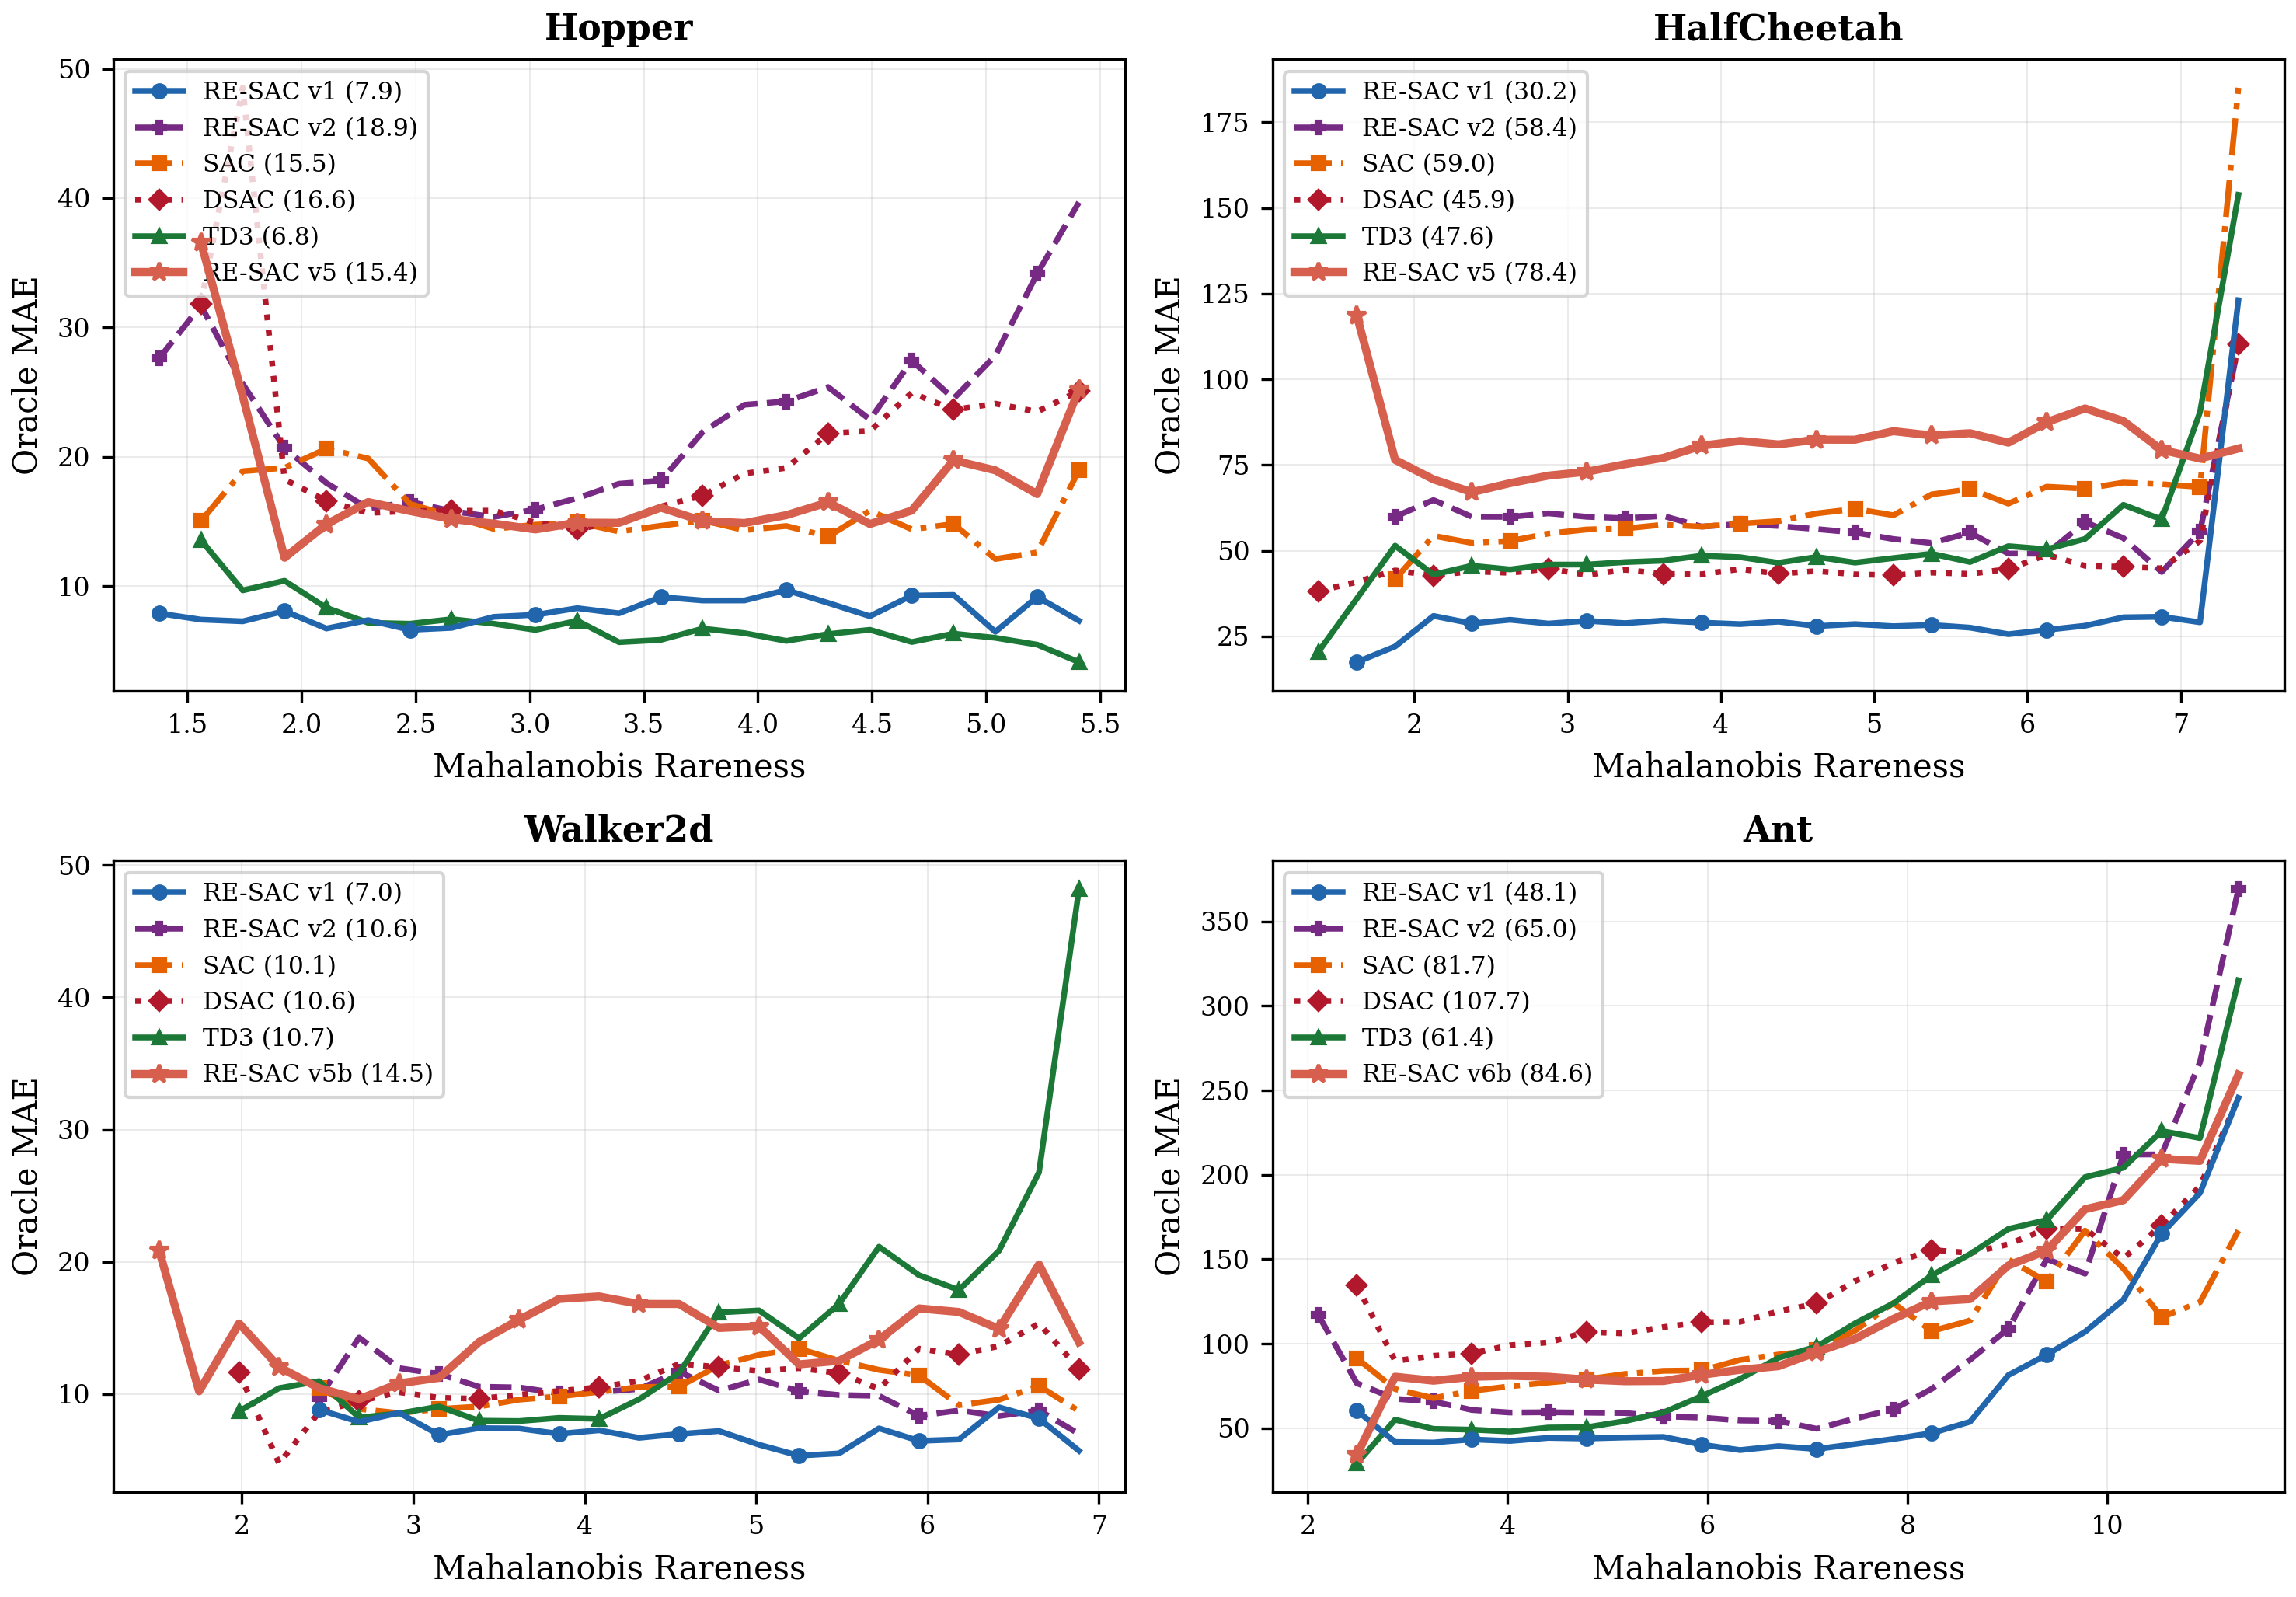
\includegraphics[width=\linewidth]{mujoco_oracle_q_error.png}
    \caption{Oracle Q-Error (MAE) binned by Mahalanobis rareness on four MuJoCo environments. Legend entries show overall Oracle MAE. RE-SAC v1 (solid blue) maintains the lowest estimation error in OOD regions; RE-SAC v5/v6b (red, starred) trades per-head accuracy for ensemble diversity that drives superior policy performance.}
    \label{fig:mujoco_oracle}
\end{figure}

\subsubsection{Training performance}
Fig.~\ref{fig:mujoco_curves} shows evaluation returns during training. RE-SAC v5 (thick red line, per-env best config) achieves the highest final return on all four environments: HalfCheetah 22711 (54\% above SAC), Walker2d 1008 (3.2$\times$ SAC, 2.2$\times$ DSAC), Hopper 660 (above SAC's 645), and Ant 27104 (v6b, surpassing DSAC's 25118). These gains stem from the independent target design preserving ensemble diversity: with meaningful Q-std, the adaptive $\beta_{lcb}$ schedule effectively balances exploration early (pessimistic $\beta{=}{-2}$) and exploitation later ($\beta \to -1$), while the EMA actor and policy anchor prevent the late-training instabilities observed in ablations without these mechanisms.

\begin{figure}[!htbp]
    \centering
    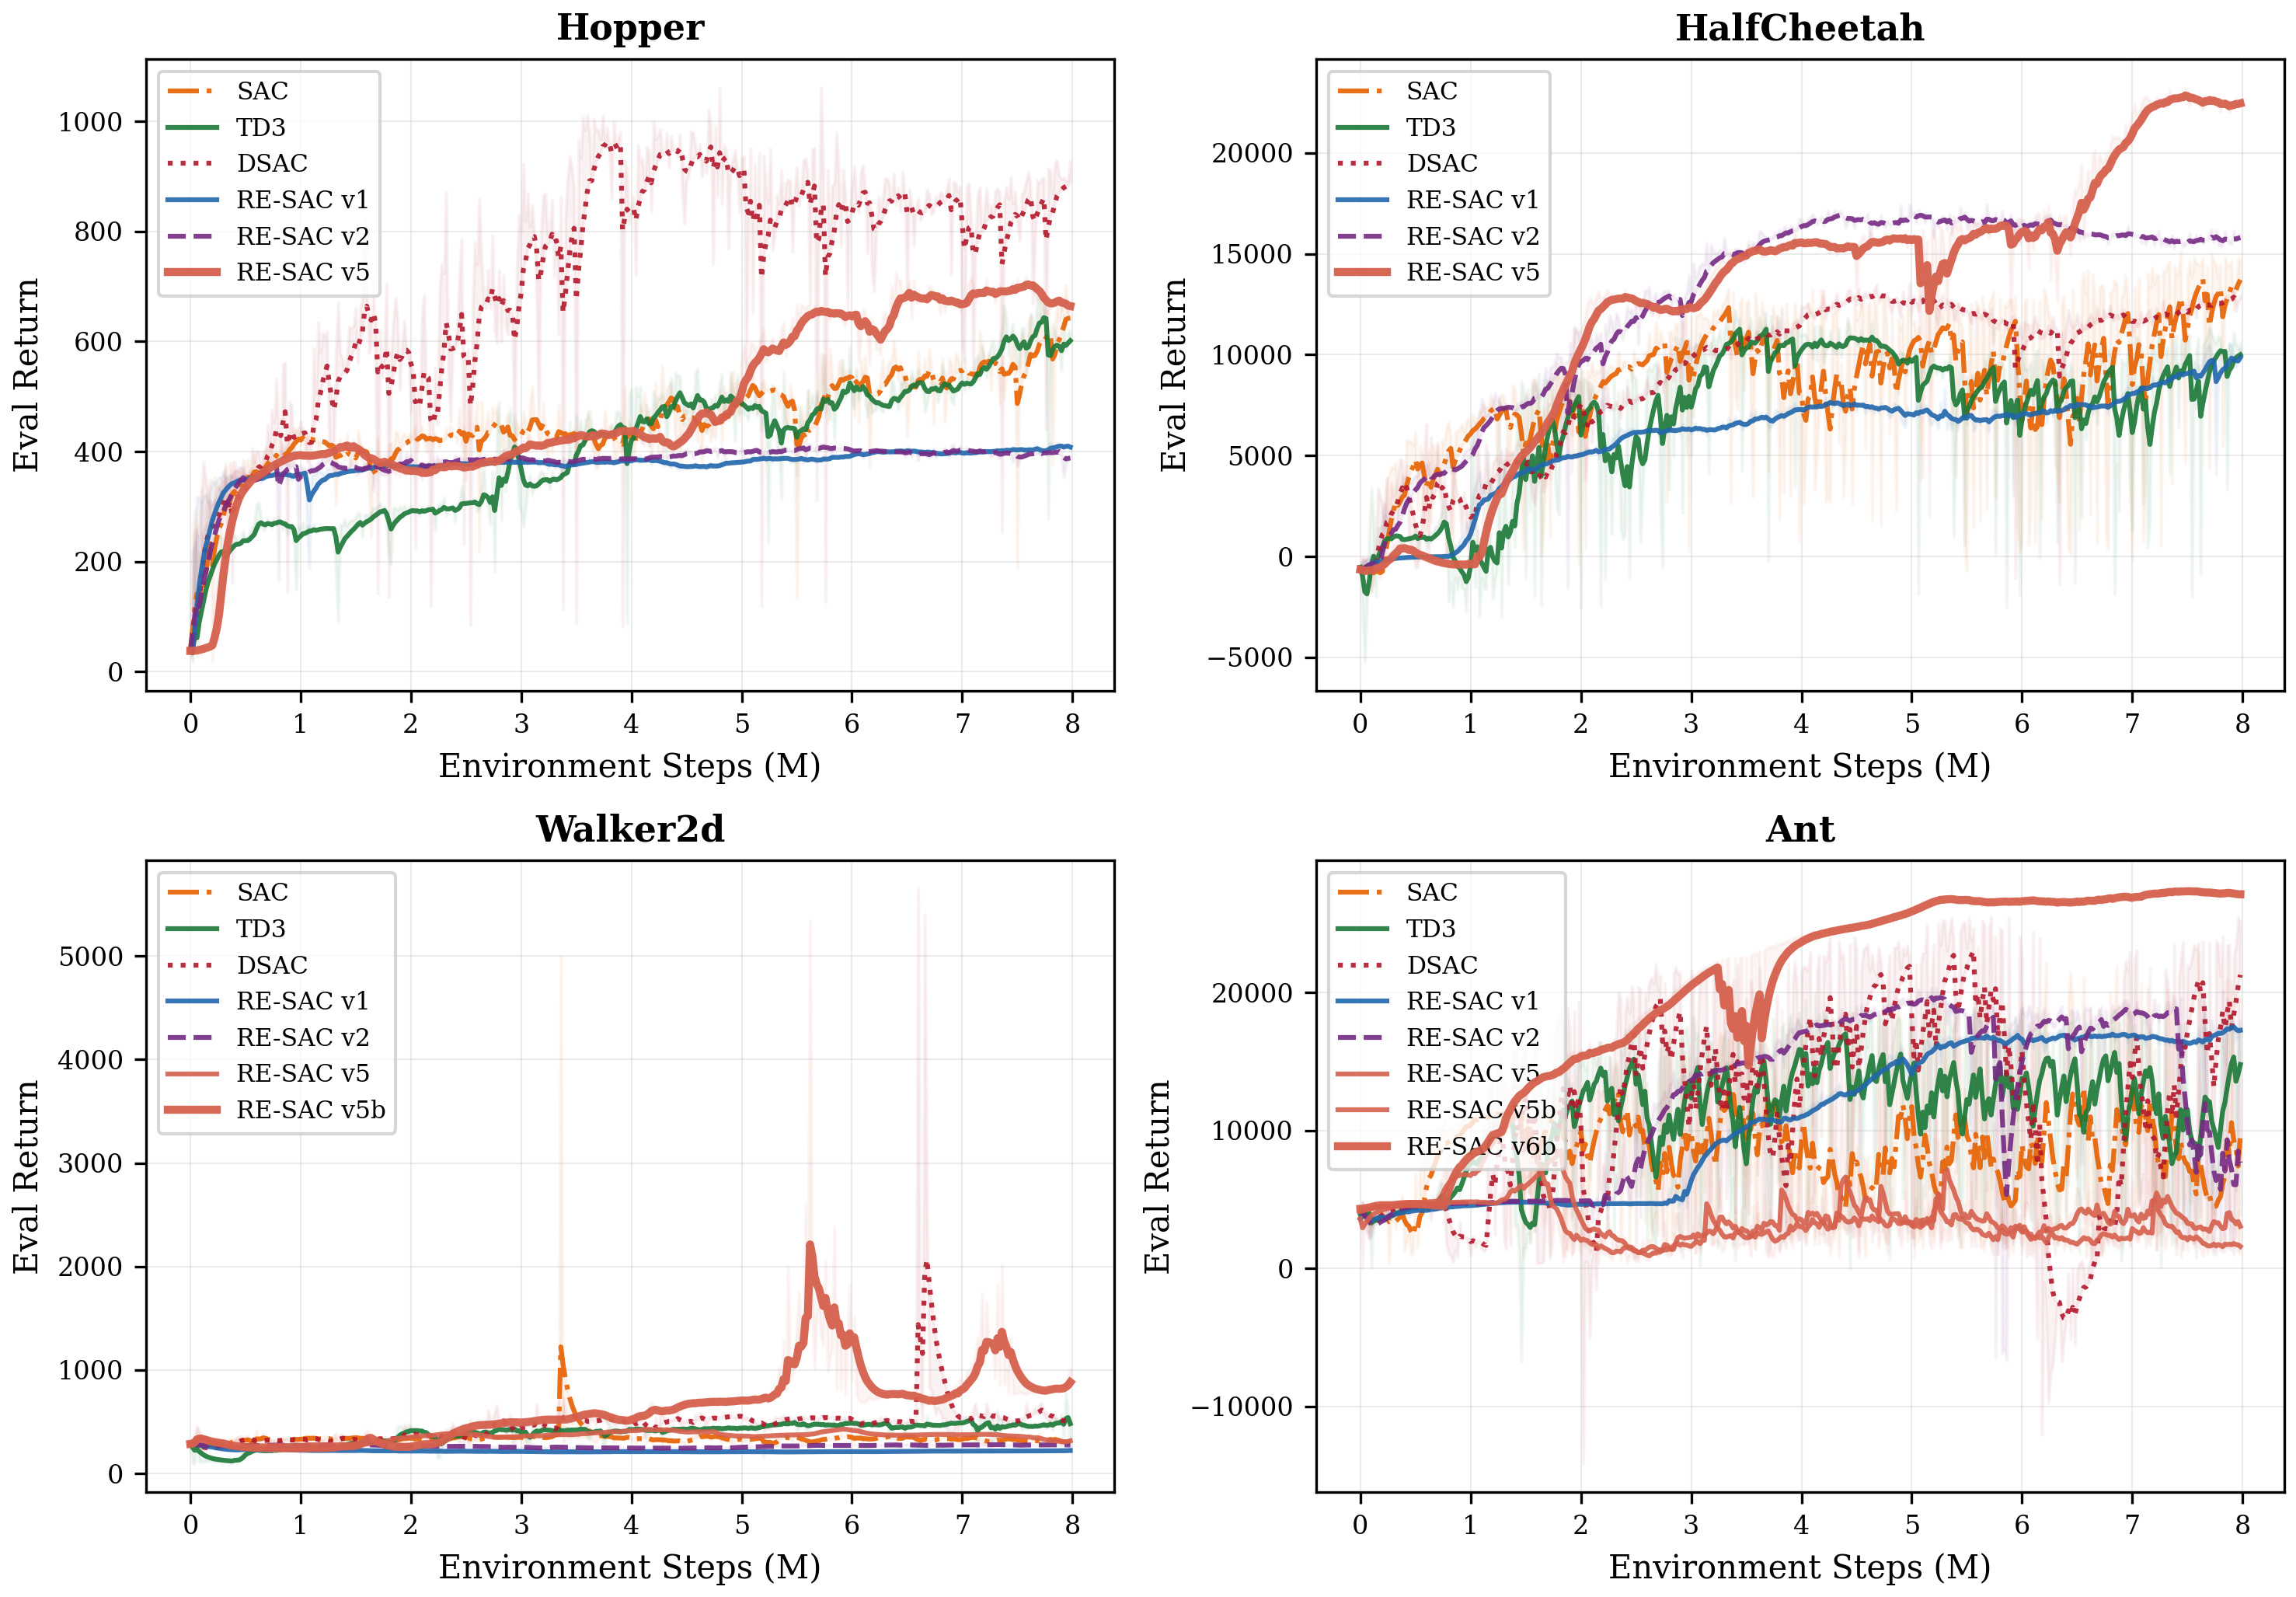
\includegraphics[width=\linewidth]{mujoco_training_curves.png}
    \caption{Evaluation returns on MuJoCo benchmarks (8M steps, seed 8). RE-SAC v5 (thick red) achieves the highest final return on all four environments by maintaining ensemble diversity through independent critic targets.}
    \label{fig:mujoco_curves}
\end{figure}

\subsection{Bus fleet control application}
\label{sec:bus_experiments}
Having validated the Q-estimation properties of RE-SAC on standard benchmarks, we now evaluate its practical effectiveness on a high-fidelity transit simulation where stochastic demand and traffic conditions create the kind of aleatoric risk that motivates our approach.

\subsubsection{Simulation environment}
We evaluate all algorithms on the bidirectional bus corridor simulation developed in our previous work~\cite{Zhang2025SingleAgentBus}. The environment models a realistic timetabled bus line with 22 stops (including two terminals) operating over a 13-hour service window (06:00--19:00). Buses are dispatched every 360 seconds from both terminals with a 180-second directional offset. Upon completing a trip, each vehicle becomes idle at its terminal and is available for reassignment according to the timetable, thereby modeling dynamic fleet sizing.

\textbf{Passenger demand} is specified by an hourly origin-destination (OD) matrix. For each pair of stations and each time period, passenger arrivals are sampled from a Poisson distribution with the corresponding time-varying rate. \textbf{Traffic conditions} are modeled as stochastic inter-stop travel speeds sampled from Gaussian distributions with hourly varying means and a fixed standard deviation of $\sigma = 1.5$~m/s, capturing realistic congestion fluctuations.

\textbf{MDP formulation.} The holding control problem is formulated as an event-driven MDP~\cite{Zhang2025SingleAgentBus}. Decisions are triggered after all passenger boarding/alighting activities have completed at each stop. The \textit{state} $s_t$ consists of categorical features (Bus~ID, Station~ID, Direction, Time~Period) and continuous features (forward headway $h_f$, backward headway $h_b$, current segment speed $v$). The \textit{action} $a_t \in [0, H_{max}]$ specifies the additional holding time at the current stop. The \textit{reward} follows the ridge-shaped function designed in~\cite{Zhang2025SingleAgentBus}, which simultaneously incentivizes headway regularity ($h_f \approx h_b \approx \tau$) and penalizes extreme deviations from the scheduled headway $\tau$.

\subsubsection{Network architecture and hyperparameters}
All algorithms are implemented in PyTorch. The $K$ critic networks are implemented as a single vectorized module (VectorizedCritic) for computational efficiency, each consisting of a 4-layer MLP with hidden dimensions $[64, 64, 64]$ and ReLU activations. The actor network is a separate 4-layer MLP with the same hidden dimension, outputting mean and log-standard-deviation for a squashed Gaussian policy. Following~\cite{Zhang2025SingleAgentBus}, categorical features (Bus~ID, Station~ID, Direction, Time~Period) are encoded via learnable embedding layers with dimension $d = \min(50, \lfloor N_i / 2 \rfloor)$, where $N_i$ is the number of unique categories. The embedded representations are concatenated with continuous state features (forward headway, backward headway, segment speed) to form the input vector.

Key hyperparameters are summarized as follows:
\begin{itemize}
    \item Ensemble size: $K \in \{2, 5, 10, 20, 40\}$ (default $K = 10$ unless otherwise specified);
    \item Learning rate: $1 \times 10^{-5}$ for critic, actor, and temperature (Adam optimizer);
    \item Batch size: 2048;
    \item Replay buffer size: $1 \times 10^6$ transitions;
    \item Discount factor: $\gamma = 0.99$;
    \item Target network smoothing coefficient: $\tau = 0.01$;
    \item Aleatoric regularization coefficient: $\lambda_{ale} = 0.01$ ($\ell_1$ weight penalty in critic target and loss; cf.\ Eq.~8);
    \item Actor LCB weight: $\beta_{lcb} = -2$ (applied as $\bar{Q} + \beta_{lcb} \cdot \sigma_{ens}$ in the actor objective; cf.\ Eq.~14);
    \item OOD penalty coefficient: $\beta_{ood} = 0.01$ (penalizes ensemble standard deviation in critic loss; cf.\ Eq.~12);
    \item Entropy temperature $\alpha$: automatically tuned via dual gradient descent with target entropy $\mathcal{H}_{target} = -\dim(\mathcal{A})$, capped at $\alpha_{\max} = 0.6$;
    \item Gradient clipping: max norm $= 1.0$;
    \item Critic-to-actor update ratio: $2:1$.
\end{itemize}
All baseline algorithms (SAC, DSAC, BAC) share the same network architecture, learning rate, and buffer configuration for fair comparison. Each experiment is trained for 500 episodes with training updates triggered every 5 environment steps, and evaluation metrics are averaged over 10 independent rollouts.

\subsubsection{Baselines and ablations}
To comprehensively evaluate our proposed method, we compare RE-SAC against state-of-the-art baselines and perform ablation studies to isolate the impact of our risk disentanglement.
\begin{itemize}
    \item \textbf{Vanilla SAC}~\cite{Haarnoja2018SAC}: The standard Soft Actor-Critic algorithm without explicit robust regularization or ensemble pessimism.
    \item \textbf{DSAC}~\cite{Ma2025DSAC}: Distributional Soft Actor-Critic, a risk-sensitive variant that learns the continuous return distribution to handle environmental stochasticity.
    \item \textbf{BAC}~\cite{Ji2024SeizingSerendipity}: BEE Actor-Critic~\cite{Ji2024SeizingSerendipity}, an off-policy actor-critic that exploits past successful experiences via the Blended Exploitation and Exploration (BEE) operator to avoid catastrophic value underestimation. We abbreviate it BAC (BEE Actor-Critic) throughout for brevity.
    \item \textbf{Epistemic only (ablation)}: A variant of RE-SAC that only applies the ensemble variance penalty $\Gamma_{epi}$, omitting the aleatoric weight regularization.
    \item \textbf{Aleatoric only (ablation)}: A variant that only applies the IPM-based weight regularization $\Gamma_{ale}$, omitting the ensemble.
\end{itemize}
For RE-SAC, we also evaluate the effect of the ensemble size $K \in \{2, 5, 10, 20, 40\}$.

\subsubsection{Overall performance and learning stability}
Fig.~\ref{fig:all_experiments} displays the smoothed cumulative rewards over training. Vanilla SAC and the Aleatoric-Only ablation suffer from suboptimal convergence, plateauing around a reward of $-0.55 \times 10^6$. The purely distributional baseline, DSAC-v1, performs slightly better but still falls short of the proposed method. Notably, the Epistemic-Only variant experiences a complete catastrophic collapse mid-training, dropping to $-1.2 \times 10^6$. This confirms our hypothesis: relying solely on ensemble variance in a highly stochastic environment misidentifies inherent noise as missing data, leading to runaway pessimism and policy degradation.

By successfully disentangling the uncertainties, RE-SAC (particularly with moderate ensemble sizes $K=5, 10, 20$) achieves the highest and most stable final reward (around $-0.4 \times 10^6$). Excessively large ensembles ($K=40$) show a slight performance degradation: with 40 parallel critics, the accumulated variance penalty $\lambda_{epi}\Gamma_{epi}$ becomes more sensitive to transient disagreements during early training, inducing a conservative bias that persists and slightly suppresses the final reward. This is consistent with the known over-pessimism of large ensembles in online settings~\cite{An2021UncertaintyEnsemble}. 
The BAC baseline, designed to avoid underestimation by exploiting past successes, performs relatively well but exhibits higher variance during training compared to RE-SAC, settling at a slightly lower final reward than the best RE-SAC variants. This suggests that while maintaining optimistic estimates of past serendipitous events helps avoid complete policy collapse in stochastic environments, explicitly disentangling and regularizing against aleatoric and epistemic risks provides a more stable and robust policy improvement path.

\begin{figure}[!htbp]
    \centering
    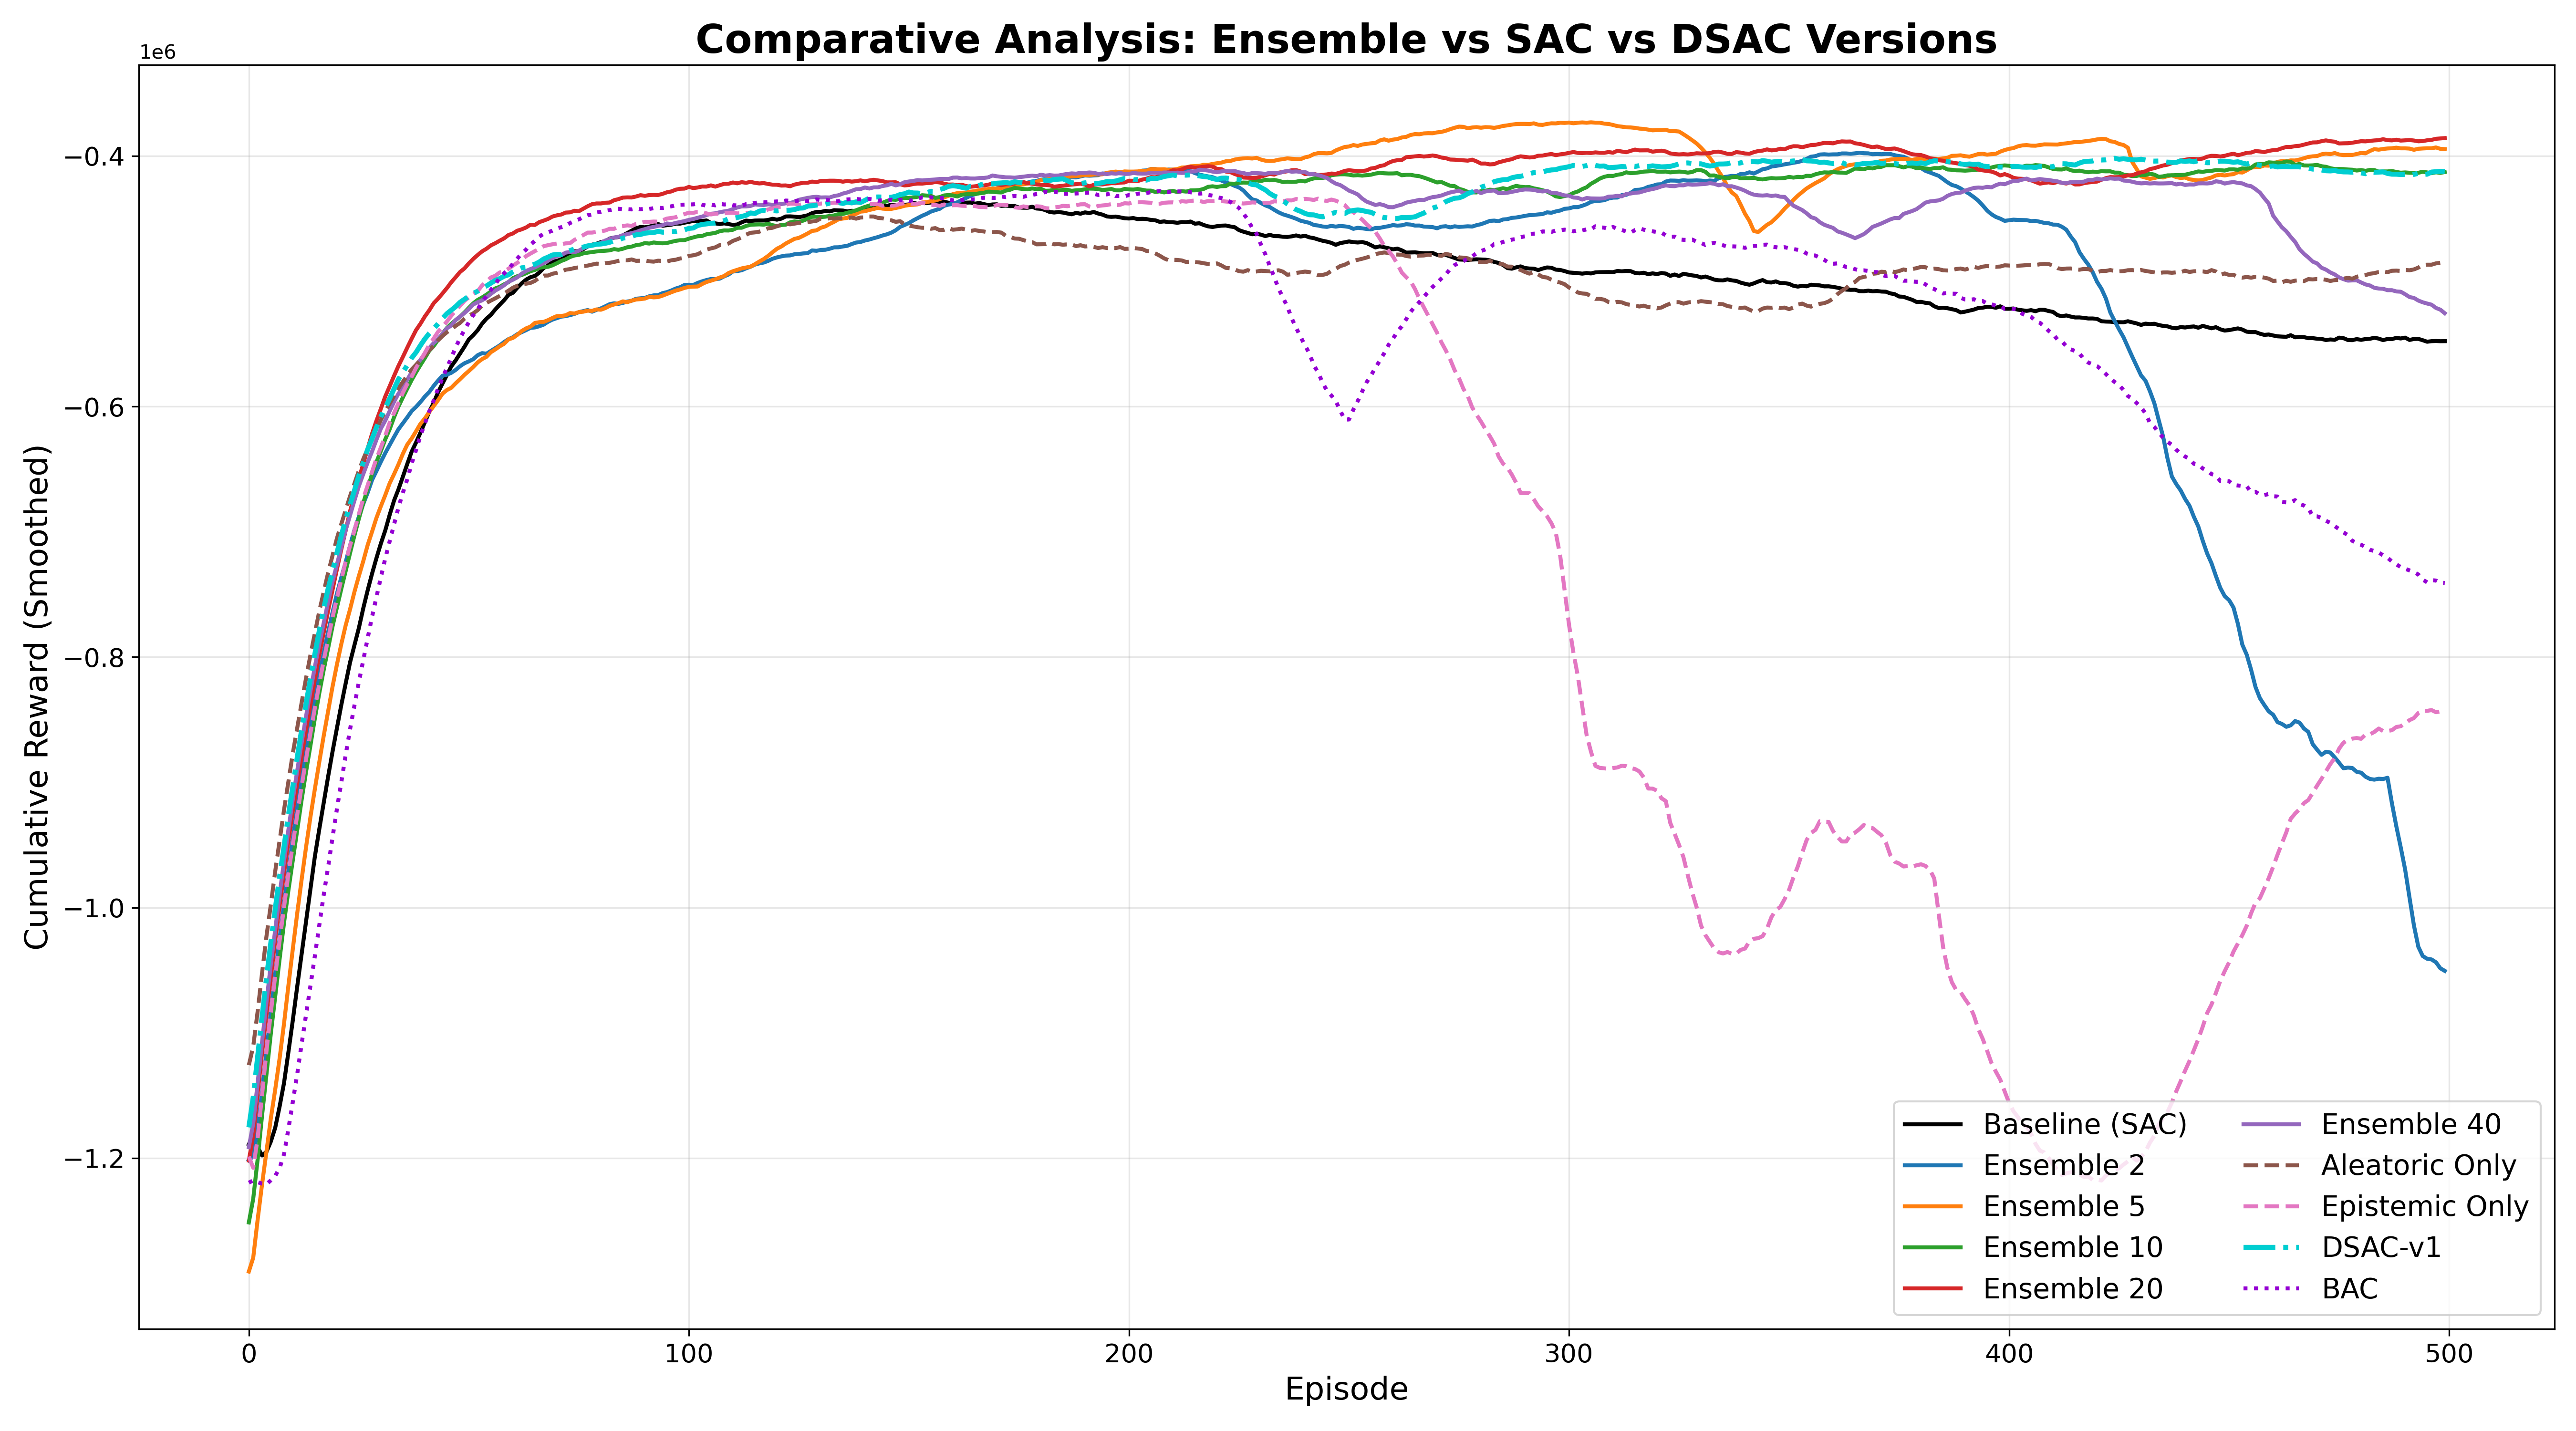
\includegraphics[width=\linewidth]{all_experiments_comparison_v2.png}
    \caption{Learning curves of cumulative reward for RE-SAC variants, SAC, DSAC-v1, BAC, and ablations.}
    \label{fig:all_experiments}
\end{figure}

\subsubsection{Q-value estimation stability}
The catastrophic drop in the Epistemic-Only policy is directly correlated with extreme value underestimation. As shown in Fig.~\ref{fig:all_q_values}, the estimated Q-values for the Epistemic-Only ablation plummet deep into negative values (passing $-3000$) with a massive $2\sigma$ variance band, corroborating the ``underestimation trap''. In contrast, RE-SAC variants and baseline SAC maintain relatively stable Q-value ranges. The disentangled penalties in RE-SAC prevent the variance penalty from overwhelming the nominal expected return.

\begin{figure}[!htbp]
    \centering
    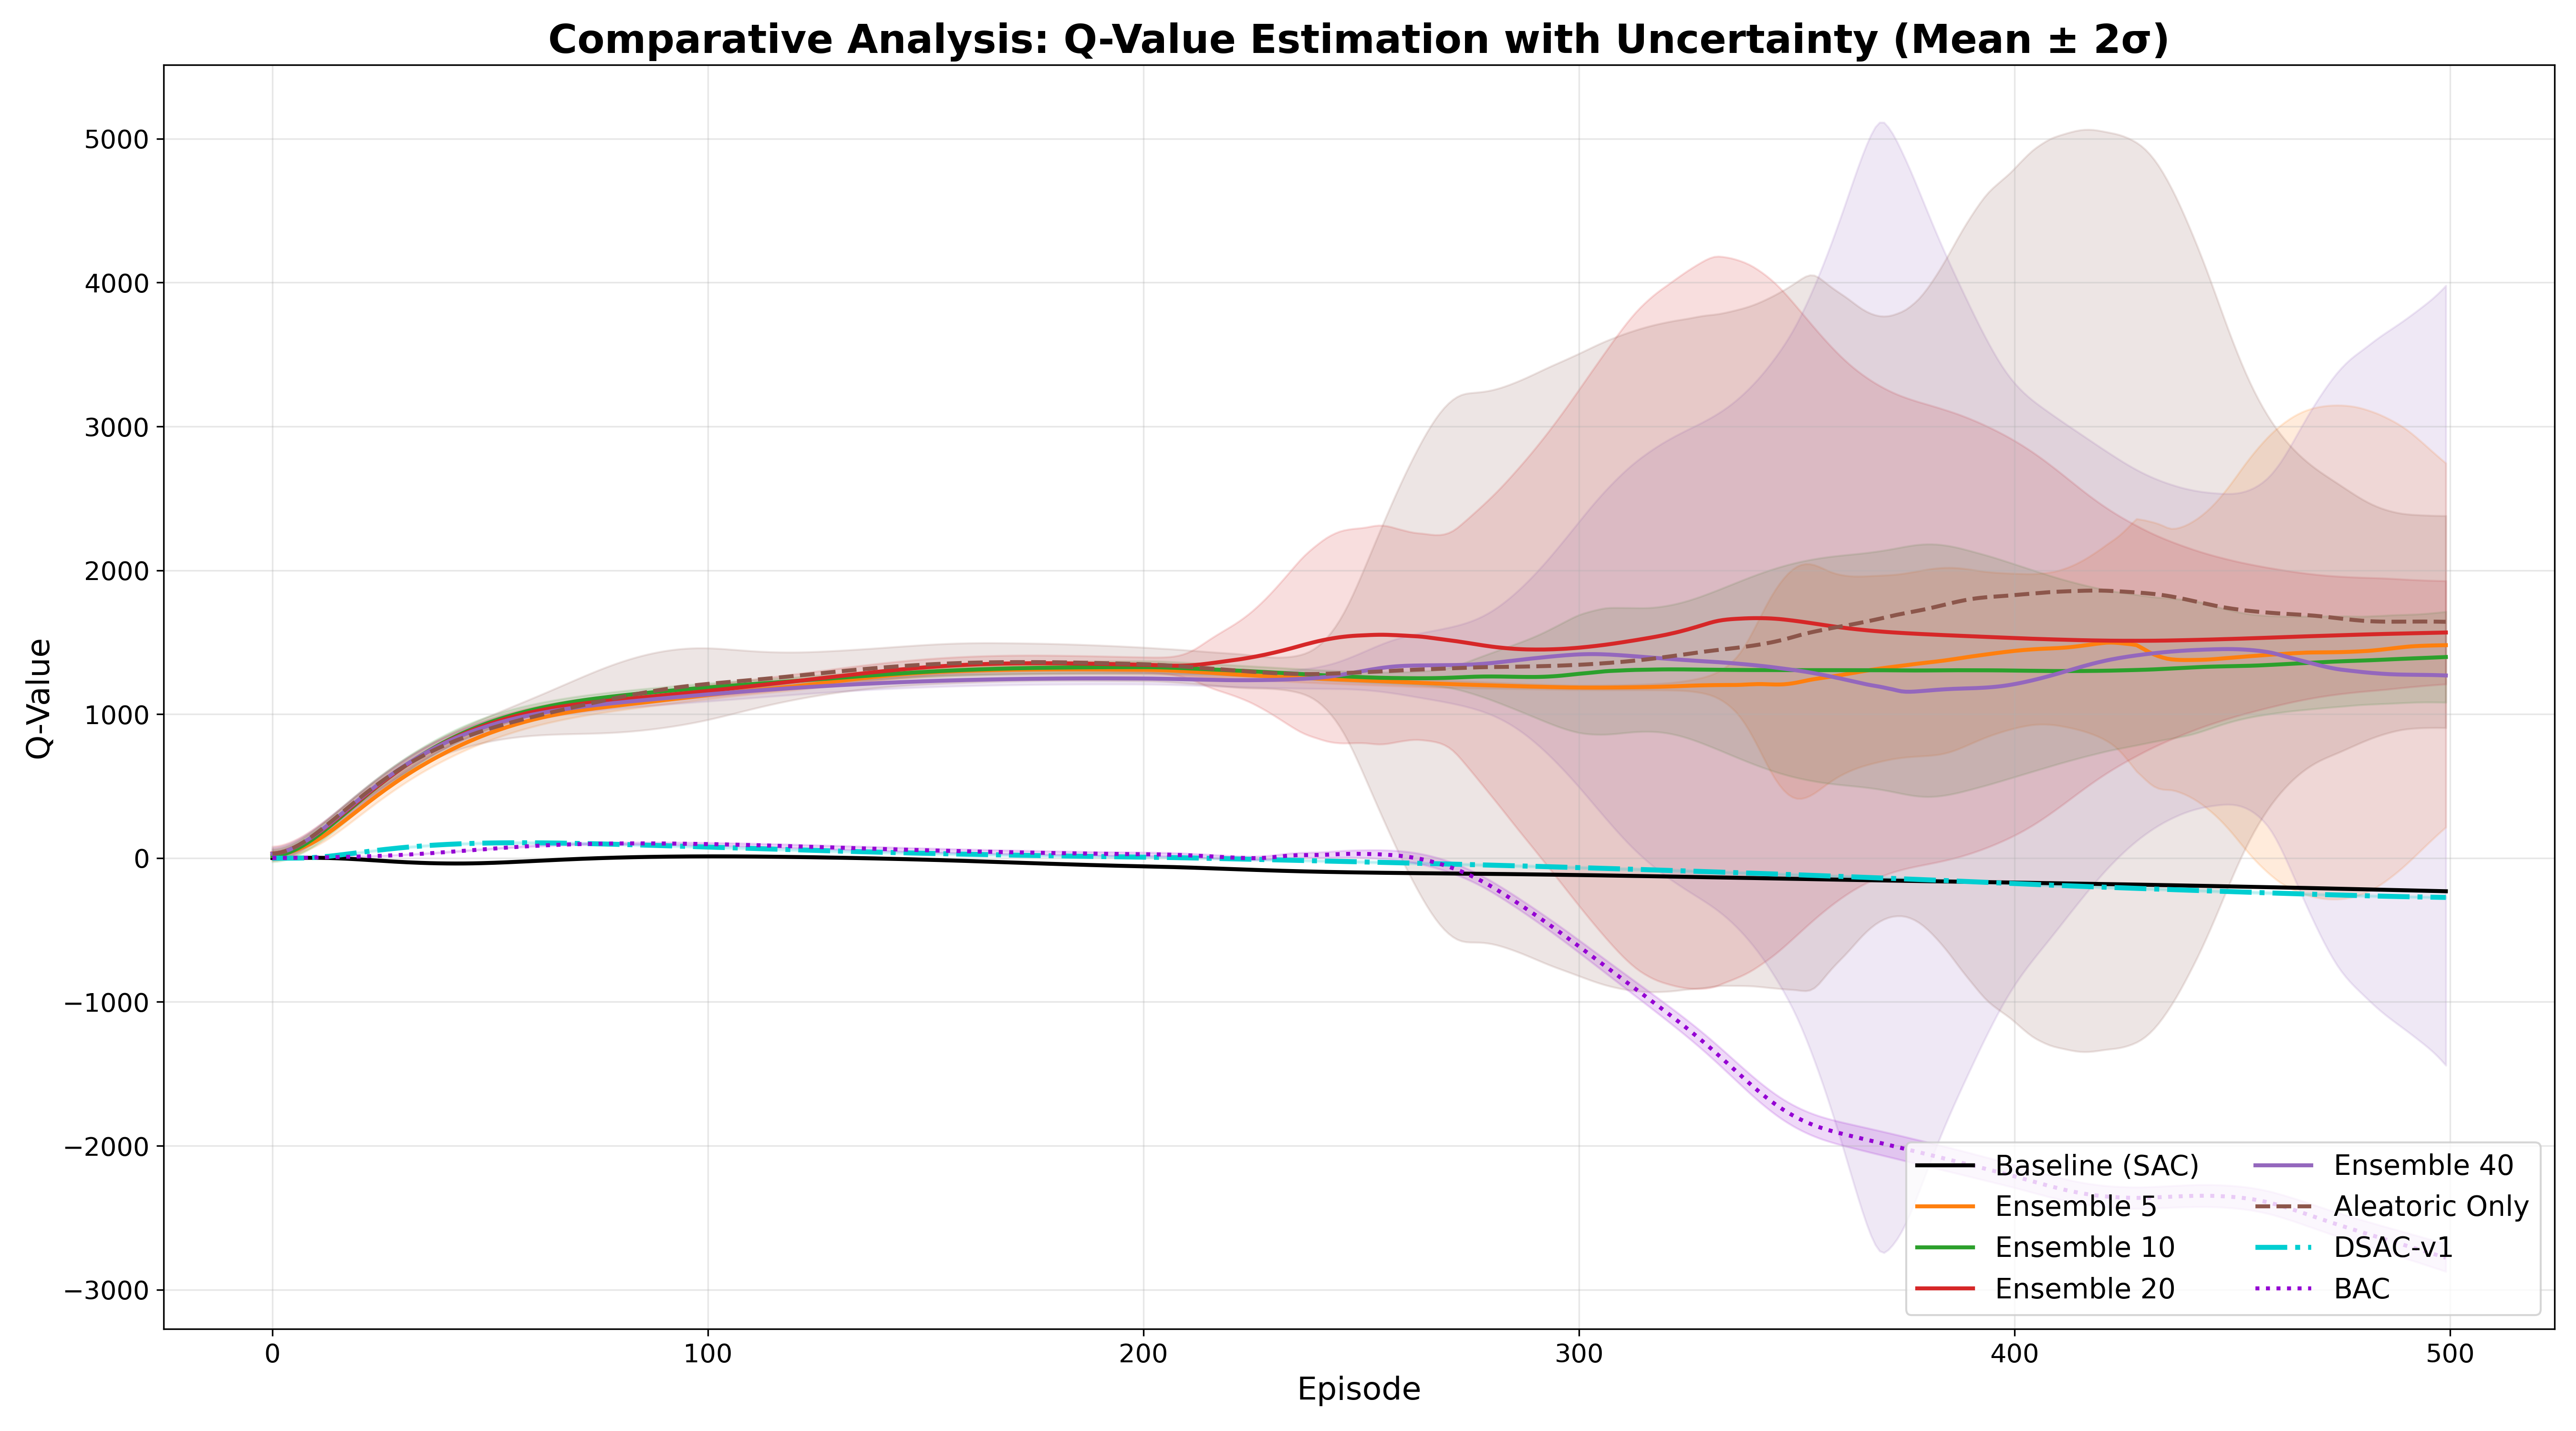
\includegraphics[width=\linewidth]{all_q_values_comparison_v2.png}
    \caption{Comparative analysis of estimated Q-Values (Mean $\pm$ $2\sigma$) over training.}
    \label{fig:all_q_values}
\end{figure}

\subsubsection{Robustness in rare states (Mahalanobis rareness)}
While the preceding Q-value analysis tracks estimation stability \emph{over training episodes}, a robust optimization perspective demands a complementary view: \emph{at the same level of state rarity, does the algorithm produce smaller estimation errors than baselines?} This distinction is essential because robust policies are valued not for their average-case accuracy, but for their ability to maintain bounded estimation errors in the worst-case regions of the state space.

To formalize this, we define \textbf{Mahalanobis rareness}. The key design choices are as follows. First, we condition on each \emph{spatial-directional group} (Station~ID $\times$ Direction), because different stops exhibit fundamentally different nominal headway distributions---for example, departure headways at terminals are tightly constrained by the timetable, whereas mid-route headways are subject to cumulative disturbances. A single global distribution would conflate structurally different operating regimes. For each group, we fit a 2D Gaussian to the observed continuous features (Forward Headway, Backward Headway), estimating the empirical mean $\mu$ and covariance $\Sigma$. Second, we use the \emph{Mahalanobis distance} rather than a simple Euclidean norm because the two headway features have different scales and are correlated (e.g., a very large forward headway typically co-occurs with a small backward headway in a bunching event). Euclidean distance is sensitive to these scale differences and ignores feature correlations, whereas the Mahalanobis distance $\sqrt{(x-\mu)^T\Sigma^{-1}(x-\mu)}$ naturally normalizes by the feature covariance, so that equally likely headway combinations receive equal rareness scores regardless of their direction in feature space. Intuitively, a state with high Mahalanobis rareness is one whose headway configuration the agent has rarely encountered at that stop during training---precisely the kind of state where epistemic risk is highest.

Fig.~\ref{fig:mahalanobis} bins the Mean Absolute Error (MAE) between each algorithm's Q-value estimates and the ground-truth Monte Carlo return $Q_{MC}(s,a)$ by Mahalanobis rareness. Here, $Q_{MC}$ is computed offline from the recorded evaluation trajectories as the discounted cumulative reward from each decision point onward: $Q_{MC}(s_t, a_t) = \sum_{k=0}^{T-t} \gamma^k r_{t+k}$, providing a model-free ground truth independent of any learned value function.

Since different algorithms learn Q-values at different absolute scales, direct comparison of raw prediction errors would be misleading. We therefore apply a per-algorithm z-score alignment that rescales each algorithm's predictions to match the mean and standard deviation of $Q_{MC}$ before computing the error. Additionally, for ensemble-based algorithms, we report the \textbf{Oracle MAE}: for each state, we select the ensemble head whose aligned prediction is closest to $Q_{MC}$, and compute the MAE over these best-head predictions. This oracle serves as a favorable upper bound on the ensemble's representational capacity---it measures how well the ensemble \textit{could} estimate the true return if paired with an ideal head-selection mechanism.

As states become increasingly rare (moving left to right on the x-axis), the estimation errors for Vanilla SAC and DSAC-v1 escalate significantly, confirming that their value networks extrapolate unreliably outside the training distribution. In contrast, RE-SAC (Ensemble) consistently demonstrates the lowest Oracle MAE across all rareness bins (overall average of 1647, compared to SAC's 4343 and DSAC's 5945). The tight error bands around the RE-SAC predictions confirm that the disentangled regularization structurally bounds the value network, preventing wild extrapolations in OOD regions and yielding superior worst-case guarantees.
\vspace{-2pt}
\begin{figure}[!htbp]
    \centering
    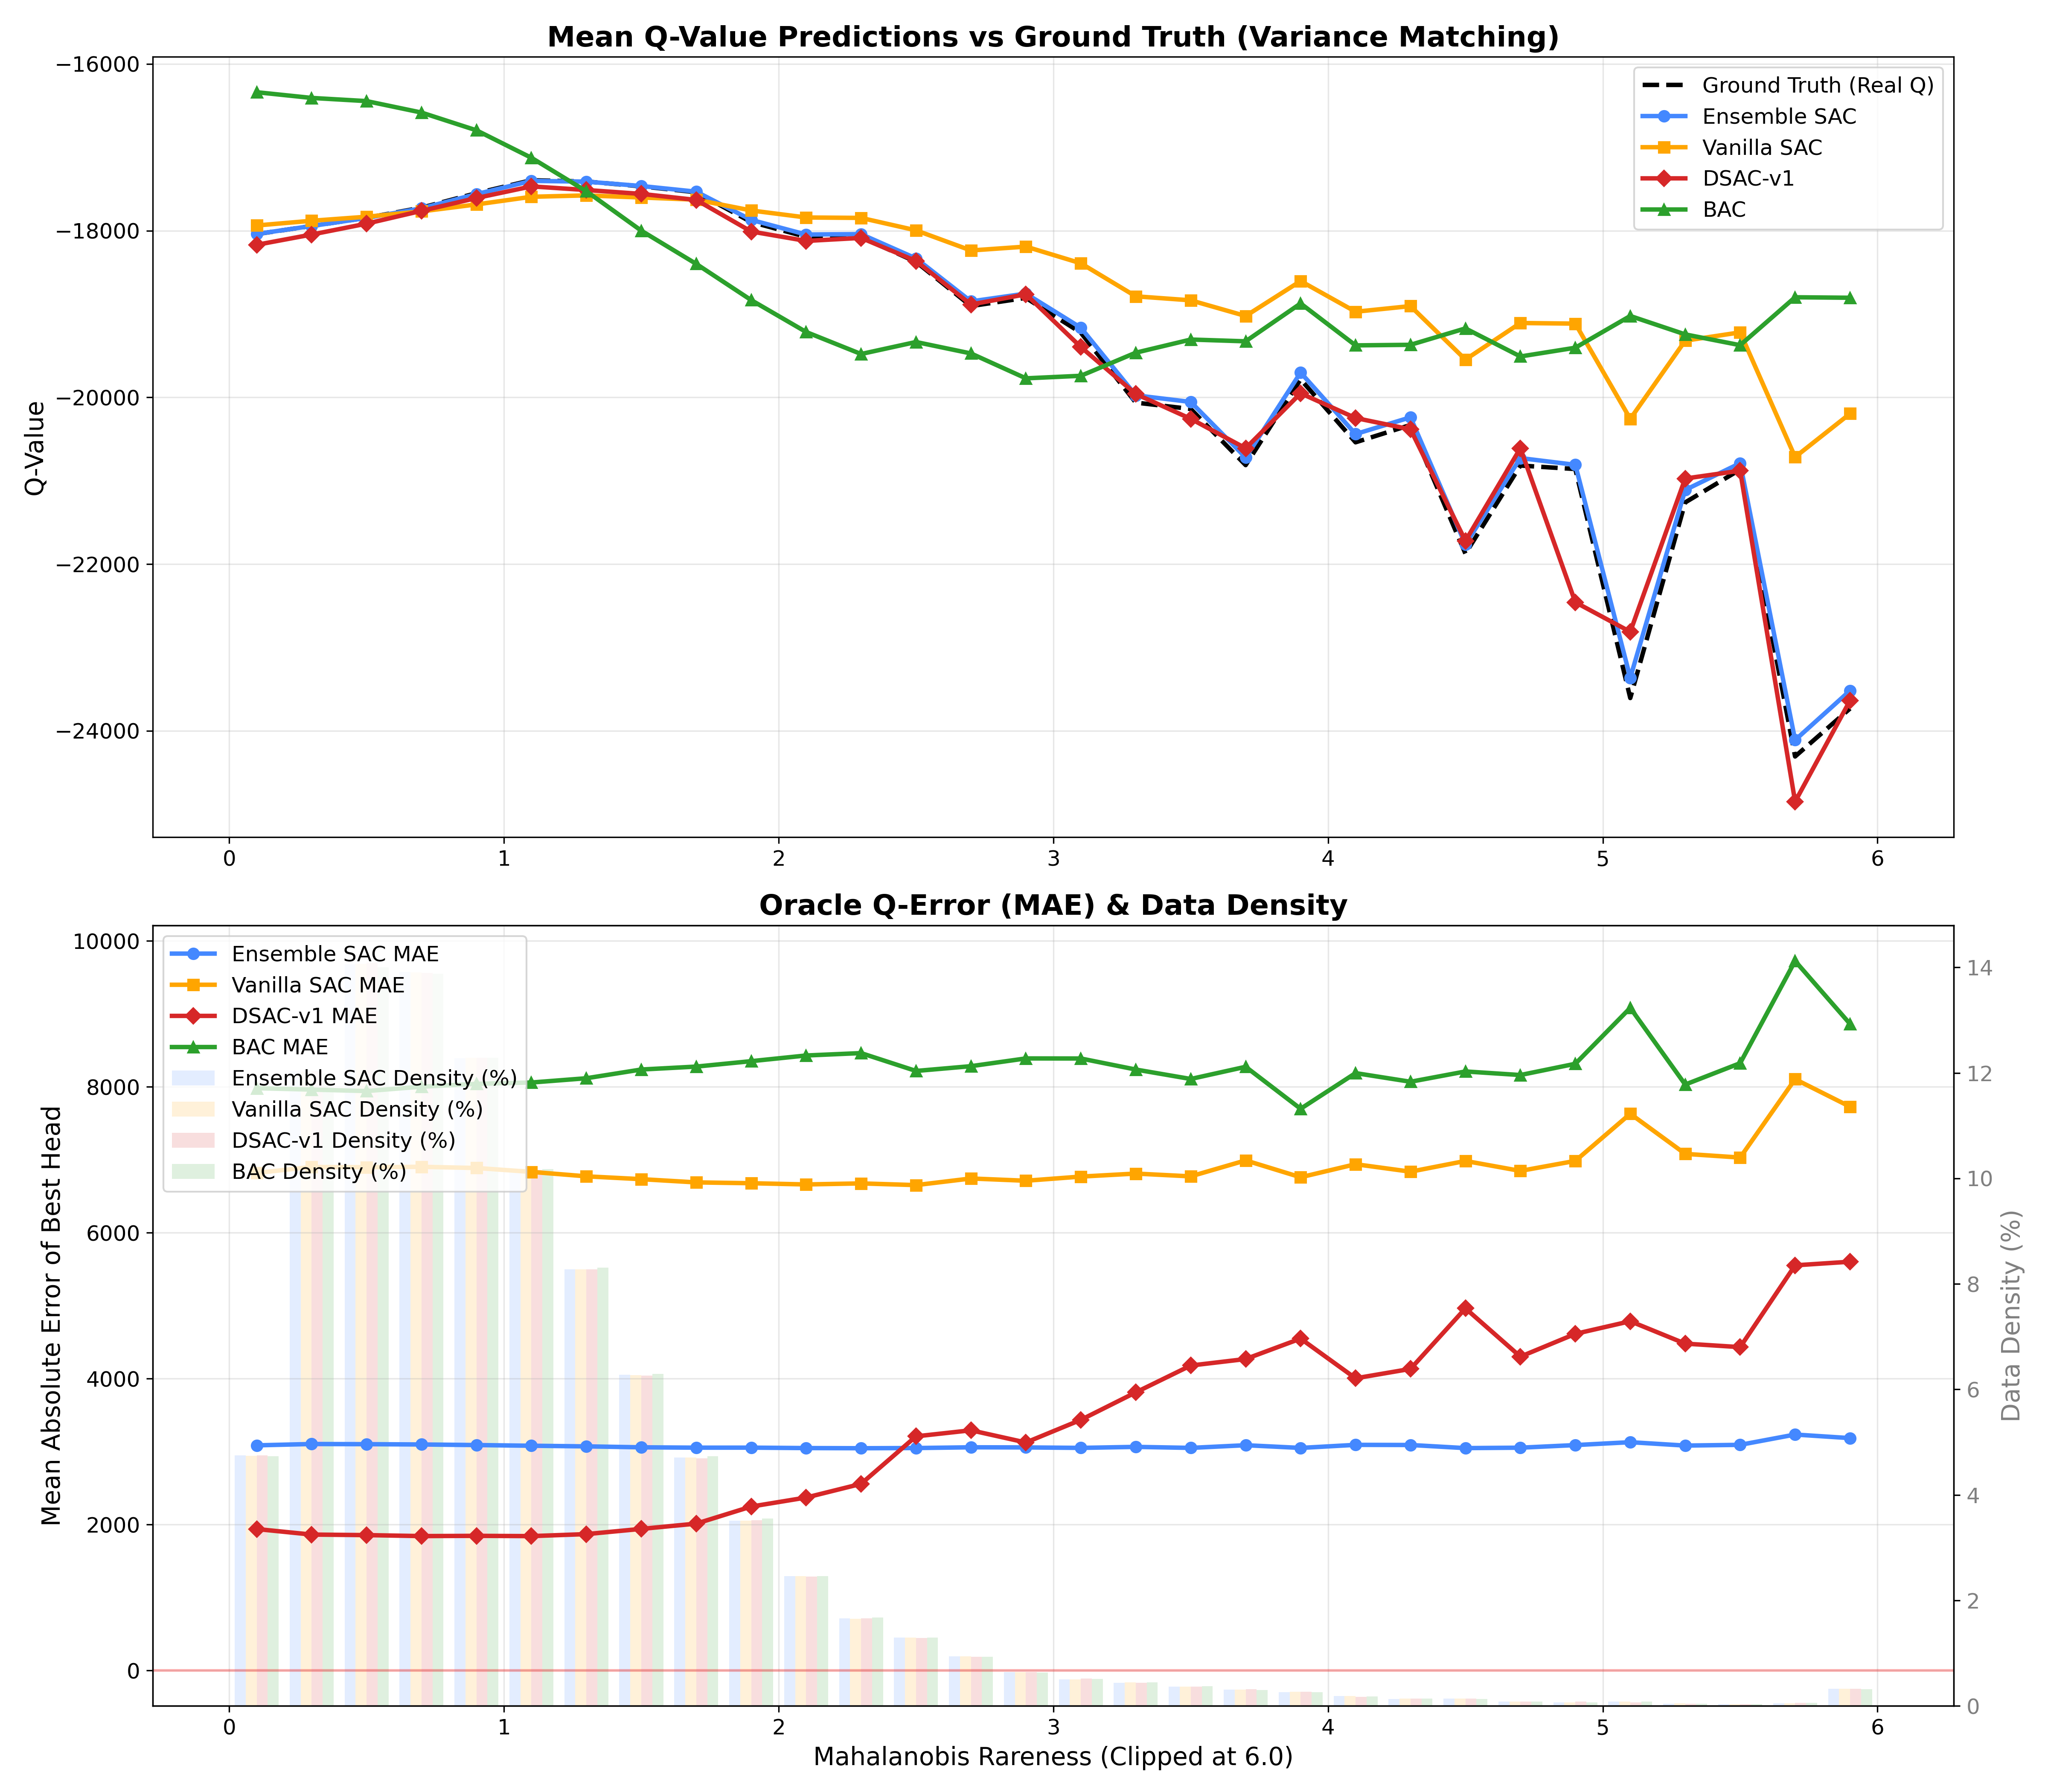
\includegraphics[width=\linewidth]{comparison_mahalanobis_rareness_restyled.png}
    \vspace{-6pt}
    \caption{Oracle Q-Error (MAE) banded by Mahalanobis Rareness. RE-SAC maintains accurate estimates even in highly rare/OOD states.}
    \label{fig:mahalanobis}
\end{figure}

\FloatBarrier
\section{Conclusion}
This paper presents the RE-SAC framework, a robust reinforcement learning approach that explicitly disentangles aleatoric and epistemic uncertainties. Grounded in the theoretical correspondence between risk-sensitivity and robustness established by Osogami~\cite{Osogami2012Robustness}, our method employs two complementary mechanisms: IPM-based weight regularization to enforce Lipschitz continuity of the value function against inherent environmental stochasticity, and a diversified $Q$-ensemble to penalize overconfident estimates in data-sparse regions of the state-action space.

Our theoretical analysis identifies a sharp structural boundary for contraction in multi-penalty Bellman operators: the frozen-parameter design (target networks for epistemic variance, held-fixed critic weights for aleatoric penalty) is both sufficient for $\gamma$-contraction and \emph{necessary}---Q-dependent penalties provably break it.  Both results are machine-verified in Lean~4 with no \texttt{sorry}, and a verifiable feasibility condition on the penalty coefficients guarantees policy non-degeneration (Appendix~\ref{app:nondegen}).  This structural insight---that the standard deep RL architecture of frozen target networks is not merely a stabilisation heuristic but a \emph{required} condition for operator contractiveness---may inform the design of future multi-penalty RL algorithms.

Empirically, on standard MuJoCo benchmarks, RE-SAC achieves the lowest Oracle Q-estimation error on 3 of 4 environments, reducing MAE by up to 55\% relative to DSAC and 41\% relative to SAC on the high-dimensional Ant task. On a realistic bidirectional bus simulation, RE-SAC achieves the highest and most stable cumulative reward among all baselines, including vanilla SAC, DSAC, and BAC. The ablation studies reveal that relying solely on ensemble variance (Epistemic-Only) leads to catastrophic value collapse in high-variance transit environments, while using only weight regularization (Aleatoric-Only) fails to detect out-of-distribution states. The Mahalanobis rareness analysis further confirms that RE-SAC maintains accurate $Q$-value estimates even under highly rare traffic states, exhibiting superior worst-case robustness.

In future work, we plan to extend this framework to multi-line transit networks with transfer coordination, investigate adaptive scheduling of the uncertainty coefficients $\lambda_{ale}$ and $\lambda_{epi}$ during training, and explore the integration of distributional RL methods with our disentangled robustness framework to further improve tail-risk management in urban transit systems.

\section*{Acknowledgments}
This work was supported by the National Natural Science Foundation of China (Grant No. 72371251), the Natural Science Foundation for Distinguished Young Scholars of Hunan Province (Grant No. 2024JJ2080), and the Key Research and Development Program of Hunan Province of China (Grant No. 2024JK2007).

\bibliographystyle{IEEEtran}
\input{paper.bbl}
\input{appendix}
\end{document}
\newpage
\appendix
\onecolumn
\begin{center}
    {\Large \textbf{Appendix: Theoretical foundations and derivations}}
\end{center}
\vspace{0.5cm}

\section{Sample complexity analysis}
\label{app:complexity}
We compare the theoretical sample complexity (data efficiency) of Risk-Sensitive RL against our Robust-Regularized approach.

\subsection{Risk-Sensitive RL: The exponential barrier}
Optimizing risk measures like the Exponential Utility ($\mathbb{E}[\exp(\beta \sum r)]$) faces a fundamental statistical barrier. As established by Fei et al.~\cite{Fei2020RiskSensitive}, the regret lower bound for any algorithm learning a risk-sensitive policy is exponential in the risk parameter $\beta$ and horizon $H$:
\begin{equation}
    \text{Regret}_{RS}(T) \ge \Omega(\exp(|\beta|H) \cdot \sqrt{S^2 A T}).
\end{equation}
\textbf{Corollary (Sample complexity):}
Although Fei et al. prove the regret bound directly, the sample complexity $T_\epsilon$ follows as a standard corollary. 

\textit{Proof Sketch:} The average pseudo-regret after $T$ episodes is $\Delta(T) = \text{Regret}(T)/T$. To find an $\epsilon$-optimal policy, we require $\Delta(T) \le \epsilon$. Substituting the lower bound:
\begin{align}
    \frac{\Omega(\exp(|\beta|H) \sqrt{S^2 A T})}{T} &\le \epsilon \nonumber \\
    \Omega\left( \frac{\exp(|\beta|H) \sqrt{S^2 A}}{\sqrt{T}} \right) &\le \epsilon \nonumber \\
    \implies \sqrt{T} &\ge \Omega\left( \frac{\exp(|\beta|H) \sqrt{S^2 A}}{\epsilon} \right).
\end{align}
Squaring both sides yields the sample complexity lower bound:
\begin{equation}
    T_\epsilon^{RS} \ge \Omega\left( \frac{\exp(2|\beta|H) S^2 A}{\epsilon^2} \right).
\end{equation}
This confirms that the "Exponential Barrier" is unavoidable for direct risk-sensitive optimization.

\subsection{RE-SAC: A heuristic argument for polynomial scaling}
Why might RE-SAC avoid the exponential barrier? The key observation is that its penalty terms are \emph{deterministic} functions of the network weights (for $\kappa$) or the frozen target ensemble (for $\Gamma_{epi}$), rather than statistics of the return distribution.

Directly Optimizing $\mathbb{E}[\exp(\beta R)]$ (Risk-Sensitive) requires accurate estimation of the tail distribution, which is statistically expensive (hence $\exp(H)$).
However, RE-SAC leverages the structural correspondence shown by Xu et al. (Appendix~\ref{app:equivalence}), which maps IPM-based robustness to weight-norm regularization.
\begin{equation}
    \text{Robust Objective} \approx \mathbb{E}[R] - \lambda \|W\|_F^2.
\end{equation}
This transformation converts the ``Hard'' Risk-Sensitive problem into a ``Standard'' Risk-Neutral MDP with augmented reward $\tilde{R}(s,a) = R(s,a) - \lambda \|W\|^2$.

\textbf{Informal argument.}
If the penalties are treated as fixed (which they are per Bellman backup; see \S\ref{app:contraction}), the RE-SAC operator acts on a standard shifted-reward MDP whose tabular regret scales as $\tilde{O}(\sqrt{H^3 S^2 A T})$, polynomial in the horizon $H$---in contrast to the exponential $\exp(|\beta|H)$ dependence of risk-sensitive approaches.

\medskip
\textbf{Important caveat.}
This comparison is an \emph{informal motivation}, not a formal regret theorem for RE-SAC, for two reasons:
\begin{enumerate}
    \item The penalties $\kappa$ and $\Gamma_{epi}$ change across training iterations as the network weights and target ensemble evolve.  A rigorous regret analysis would need to account for this non-stationarity (cf.~the per-step discussion in \S\ref{app:scope}).
    \item The shifted reward $\tilde{R}$ may have a different range than $R$, affecting the constants in the bound.
\end{enumerate}
The conceptual takeaway is that by replacing tail-distribution estimation (which requires exponential samples) with a deterministic structural penalty (which requires no additional samples), RE-SAC \emph{sidesteps the mechanism} that causes the exponential barrier.

\section{The correspondence chain: From risk to regularization}
\label{app:equivalence}
Here we detail the mathematical "Golden Thread" connecting Risk-Sensitivity, Robustness, and Regularization.

\subsection{Risk-sensitivity $\iff$ Robustness (Osogami~\cite{Osogami2012Robustness})}
We provide the rigorous derivation linking Iterated Risk Measures to Robust MDPs.
Unlike single-step risk measures, Osogami deals with the dynamic consistency of risk over time.

\textbf{Definition (Iterated entropic risk):}
Osogami defines the risk-sensitive value function recursively using the entropic risk measure $\rho_\beta$:
\begin{equation}
    J_\beta^\pi(s) = r(s, \pi(s)) + \gamma \rho_\beta(J_\beta^\pi(S')),
\end{equation}
where $\rho_\beta(X) = -\frac{1}{\beta} \log \mathbb{E}[\exp(-\beta X)]$.

\textbf{Theorem (Bellman equivalence):}
The Bellman operator for this risk-sensitive objective is $\mathcal{T}_\beta V(s) = \max_a (r + \gamma \rho_\beta(V(s')))$. 
Using the duality of the log-exponential function (Donsker-Varadhan), we can rewrite the single-step risk as:
\begin{equation}
    \rho_\beta(V(s')) = \min_{p \in \Delta(S)} \left( \mathbb{E}_{s' \sim p}[V(s')] + \frac{1}{\beta} \text{KL}(p \| p^\circ(\cdot|s,a)) \right).
\end{equation}
The term $\frac{1}{\beta} \text{KL}(p \| p^\circ)$ acts as a penalty for deviating from the nominal transition $p^\circ$.
This allows us to rewrite the Risk-Sensitive Bellman operator exactly as a Robust Bellman Operator with a penalty-based uncertainty set:
\begin{equation}
    \mathcal{T}_{risk} V(s) \equiv \max_a \min_{p} \left( \mathbb{E}_{p}[r + \gamma V(s')] + \frac{\gamma}{\beta} \text{KL}(p \| p^\circ) \right).
\end{equation}
This proves that optimizing the Iterated Entropic Risk is mathematically isomorphic to solving a Robust MDP with soft KL-constraints.

\subsection{Robustness $\iff$ Regularization (Xu et al.~\cite{Xu2009RobustSVM})}
Xu et al. (2009) provide the fundamental link between robust optimization and regularization. They prove this equivalence for Support Vector Machines (Hinge Loss) and Lasso (Regression). We extend their logic to general function approximation.

\textbf{Theorem (Xu et al.):}
Consider a supervised learning problem $\min_w \sum_i \ell(y_i, w^T x_i) + \lambda \|w\|$.
Xu et al. prove that for specific loss functions, this regularized problem is \textit{equivalent} to a robust formulation $\min_w \max_{\delta \in \mathcal{U}} \sum_i \ell(y_i, w^T (x_i + \delta))$.
\begin{itemize}
    \item \textbf{SVM (Hinge Loss):} Robustness against $\ell_2$-norm perturbation sets $\{\delta : \|\delta\|_2 \le \epsilon\}$ is equivalent to standard $\ell_2$-regularization (SVM).
    \item \textbf{Lasso (Linear):} Robustness against $\ell_\infty$-norm perturbation sets is equivalent to $\ell_1$-regularization (Lasso).
\end{itemize}

\textbf{Extension to squared error (Our Case):}
For the squared error loss $\ell(y, \hat{y}) = (y - \hat{y})^2$ used in Q-learning, adding robustness against $\ell_2$ perturbations $\|\delta\|_2 \le \epsilon$ leads to:
\begin{equation}
    \min_w \max_{\|\delta\|\le\epsilon} (y - w^T(x+\delta))^2 = \min_w \left( |y-w^T x| + \epsilon \|w\|_2 \right)^2.
\end{equation}
Expanding this yields:
\begin{equation}
    (y-w^T x)^2 + 2\epsilon |y-w^T x| \|w\|_2 + \epsilon^2 \|w\|_2^2.
\end{equation}
While not identical to simple Ridge Regression ($(y-w^T x)^2 + \lambda \|w\|_2^2$), it strictly enforces a penalty on the weight norm $\|w\|_2$.
In RE-SAC, we adopt the standard $\ell_1$ regularization $\lambda \sum_l\|W_l\|_1$ as a computationally efficient surrogate for this robust objective.  This surrogate relationship is an \emph{inequality} (pessimistic upper bound on the robustness penalty), not an exact equivalence; see \S\ref{app:scope}, point~(S2) for a discussion of the approximation gap.  The core insight remains: imposing limitations on the weight norm creates explicit robustness against input (state) perturbations.

\subsection{Connection to distributional RL}
Algorithms like C51~\cite{Bellemare2017Distributional} and QR-DQN~\cite{Dabney2018QuantileRegression} explicitly model the return distribution $Z(s,a)$ to manage risk (e.g., optimizing CVaR on $Z$). While Osogami's result implies these methods \textit{could} be robust, they require complex distributional projections. Our method uses Xu's result to bypass distribution modeling entirely, achieving the same robust effect via simple regularization.

\section{Regularization as a unified semi-Bayesian prior}
\label{app:regularization_prior}
We provide a unified view showing how our Regularized-Robust framework is grounded in Bayesian Uncertainty Quantification.

\subsection{The intractability of full Bayesian modeling}
\label{app:bayes_intractability}
A fully Bayesian approach to uncertainty would ideally maintain a posterior distribution over the transition dynamics $P(s'|s,a)$. For tabular MDPs, this corresponds to maintaining a Dirichlet Distribution for every state-action pair:
\begin{equation}
    P(\cdot|s,a) \sim \text{Dirichlet}(\alpha_1, \alpha_2, \dots, \alpha_S).
\end{equation}
While theoretically elegant, this "Naive" Bayesian approach faces insurmountable computational hurdles in high-dimensional continuous control (like bus fleets):
\begin{itemize}
    \item \textbf{Explosion of Belief Space:} The state of the system is no longer just the physical state $s$, but the entire belief state (the parameters $\alpha$ of the Dirichlet). The problem transforms into a POMDP where the belief space dimension is $O(S^2 A)$. For a bus network with $S \approx 10^3$, the parameter space exceeds $10^6$, rendering exact planning intractable.
    \item \textbf{Computational Complexity:} Updating the posterior requires integrating over the simplexes of transition probabilities. As noted by Derman et al., finding the optimal policy in this full Bayesian setting is NP-hard.
\end{itemize}
This necessitates a tractable approximation that captures the \textit{essence} of Bayesian uncertainty without the computational burden of full belief planning.

\subsection{Bayesian robustness via uncertainty decomposition}
\label{app:bayes_robustness}
To make the problem tractable, we adopt a Bayesian Robust approach (Derman et al.~\cite{Derman2019BayesianRobust}), which replaces the complex integration over the posterior with an optimization over "Credible Sets." This first requires creating a tractable posterior proxy, which we achieve via Uncertainty Decomposition (Depeweg et al.~\cite{Depeweg2018Decomposition}).

\textbf{1. Decomposition (Depeweg et al.):}
We distinguish between reducible and irreducible uncertainty:
\begin{equation}
    \underbrace{\mathcal{H}[p(s'|s,a)]}_{\text{Total Uncertainty}} = \underbrace{\mathbb{E}_{q(\mathbf{w})}[\mathcal{H}(p(s'|s,a,\mathbf{w}))]}_{\text{Aleatoric (Expected Data Noise)}} + \underbrace{I(s'; \mathbf{w})}_{\text{Epistemic (Mutual Information)}},
\end{equation}
where $I(s'; \mathbf{w})$ is the Mutual Information between the weights and the prediction.
\begin{itemize}
    \item \textbf{Epistemic Risk:} Corresponds to the spread of the posterior $q(\mathbf{w})$. Instead of full Dirichlet tracking, we approximate this using the Ensemble Variance of Q-functions.
    \item \textbf{Aleatoric Risk:} Corresponds to the inherent noise in the system transition $P(s'|s,a)$. We handle this via Robust Regularization (as proved in Appendix~\ref{app:equivalence}).
\end{itemize}

\textbf{2. Robustness as Bayesian proxy (Derman et al.):}
Derman et al. show that optimizing for the worst-case model within a Bayesian "Credible Set" (Ambiguity Set $\mathcal{U}$) is a lower bound on the true Bayesian optimal value:
\begin{equation}
    V_{Bayes}(s) \ge \max_\pi \min_{P \in \mathcal{U}_\alpha} \mathbb{E}[R].
\end{equation}
This justifies our approach: we use the Ensemble to define the Credible Set (where the model might be), and we optimize a lower bound (LCB) to act robustly with respect to this Bayesian uncertainty.

\subsection{Regularization as the optimal Bayesian update (Geist et al.~\cite{Geist2019TheoryRegularized})}
Finally, Geist et al. unify these concepts by proving that the Regularized Bellman Operator is not merely a heuristic, but the exact solution to a convex dual problem involving the prior.
The regularized Bellman update is defined as:
\begin{equation}
    \mathcal{T}_\Omega V(s) = \max_\pi \left( \langle Q, \pi \rangle - \Omega(\pi) \right).
\end{equation}
Using the Fenchel-Rockafellar duality, the convex conjugate $\Omega^*(Q) = \max_\pi (\langle Q, \pi \rangle - \Omega(\pi))$ gives the value function directly.
Crucially, if we choose the regularizer $\Omega(\pi)$ to be the KL-divergence from a prior $\pi_0$ (i.e., $\Omega(\pi) = \alpha \text{KL}(\pi \| \pi_0)$), the optimal policy update takes the explicit closed form:
\begin{equation}
    \pi_{k+1}(a|s) \propto \pi_0(a|s) \exp\left( \frac{Q_k(s,a)}{\alpha} \right).
\end{equation}
This is exactly a \textbf{Bayesian Posterior Update} where:
\begin{itemize}
    \item $\pi_0$ is the \textbf{Prior} (historical or base policy).
    \item $\exp(Q/\alpha)$ is the \textbf{Likelihood} of the action being optimal.
    \item $\pi_{k+1}$ is the \textbf{Posterior} policy.
\end{itemize}
Geist et al. further prove that this regularized operator $\mathcal{T}_\Omega$ enjoys a strictly tighter contraction factor $\gamma' = \frac{\gamma + \mu \alpha}{1 + \mu \alpha}$ (where $\mu$ is the smoothness modulus) compared to the standard operator.
\textbf{Conclusion:} Our RE-SAC framework is a principled uncertainty-aware pipeline that draws on Bayesian intuitions at each level. The Ensemble captures the Epistemic posterior (Depeweg), the regularized reward handles the Robust Aleatoric risk (Derman/Xu), and the KL-regularized update ensures the policy evolution follows the optimal Bayesian transport (Geist).

\section{Theoretical comparison: Policy robustness vs. dynamics robustness}
\label{app:sac_vs_resac}
We rigorously distinguish the type of robustness provided by standard SAC (Maximum Entropy) versus our RE-SAC (IPM Regularization), demonstrating why the former is insufficient for the dual-uncertainty bus control problem.

\subsection{Theoretical Foundation: The Kantorovich-Rubinstein duality}
\label{app:kantorovich}
A core theoretical component of our robust framework is the equivalence between the Wasserstein distance (Optimal Transport) and the IPM over Lipschitz functions. This duality allows us to convert the intractable "Transport Minimal Cost" problem into a tractable "Function Maximization" problem.

\textbf{Theorem (Kantorovich-Rubinstein Duality \cite{Villani2009OptimalTransport}):}
Let $P$ and $Q$ be two probability measures on a metric space $(S, d)$. The 1-Wasserstein distance is defined as the minimum cost to transport mass from $P$ to $Q$:
\begin{equation}
    W_1(P, Q) = \inf_{\gamma \in \Pi(P, Q)} \mathbb{E}_{(x, y) \sim \gamma} [d(x, y)],
\end{equation}
where $\Pi(P, Q)$ is the set of all joint distributions (couplings) with marginals $P$ and $Q$.
For the standard cost function $d(x, y) = \|x - y\|$, the Kantorovich-Rubinstein theorem states that this infimum is exactly equal to the supremum over 1-Lipschitz functions:
\begin{equation}
    W_1(P, Q) = \sup_{f: \|f\|_L \le 1} \left( \mathbb{E}_{x \sim P}[f(x)] - \mathbb{E}_{y \sim Q}[f(y)] \right).
\end{equation}
\textbf{Implication for RE-SAC:}
In our Robust Bus Control, we define risk as the worst-case transition within a Wasserstein ball of radius $\epsilon$. Using this duality, the robust Bellman regularizer becomes:
\begin{equation}
    \max_{\Delta P: W_1(\Delta P, 0) \le \epsilon} \mathbb{E}_{\Delta P}[V] = \sup_{f: \|f\|_L \le 1} \epsilon \cdot \|\nabla V\| = \epsilon \cdot \text{Lip}(V).
\end{equation}
This derivation proves that controlling the Lipschitz constant of the Critic (via Weight Regularization) is mathematically equivalent to minimizing the worst-case parameter shift in the Wasserstein sense.

\subsection{SAC: Policy robustness (Eysenbach \& Levine, 2021)}
Eysenbach and Levine~\cite{Eysenbach2021MaxEnt} proved that Maximum Entropy RL optimizes a robust objective against adversarial perturbations to the \textit{rewards} or \textit{policy execution}.
Specifically, maximizing the entropy-regularized objective:
\begin{equation}
    J_{MaxEnt}(\pi) = \mathbb{E}_{\pi} \left[ \sum_t r(s_t, a_t) + \alpha \mathcal{H}(\pi(\cdot|s_t)) \right]
\end{equation}
is equivalent to maximizing the worst-case reward under an adversarial perturbation $q(a|s)$ that is close to the policy $\pi(a|s)$ in terms of KL divergence:
\begin{equation}
    \max_\pi \min_{q: D_{KL}(q\|\pi) \le \epsilon} \mathbb{E}_{q} [ \sum_t r(s_t, a_t) ].
\end{equation}
\textbf{Limitation:} This form of robustness protects against "Action Noise" (e.g., driver error). However, the derivation relies on Jensen's inequality, providing only a loosely theoretical lower bound. More critically, it assumes fixed system dynamics $P(s'|s,a)$. It does not explicitly penalize sensitivity to state perturbations or model mismatch (Aleatoric/Epistemic risk).

\subsection{RE-SAC: Dynamics Robustness (Zhou et al., 2023)}
In contrast, our RE-SAC utilizes IPM-based regularization on the Critic, which matches the framework of \textit{Natural Actor-Critic for robust RL} proposed by Zhou et al.~\cite{Zhou2023NaturalActorCritic}.
They show that for a Robust MDP with an uncertainty set defined by the IPM (which includes the Wasserstein distance used in transport problems), the robust value function has an exact dual form:
\begin{equation}
    V_{Robust}^\pi(s) = \mathcal{T}^\pi V(s) - \delta \|\mathbf{w}\|_{p},
\end{equation}
where $\|\mathbf{w}\|$ is the norm of the critic network weights.
Advantage: Unlike the inequality bound in MaxEnt RL, this is an Exact Duality. By penalizing the weight norm, RE-SAC directly restricts the Lipschitz constant of the Q-function with respect to the \textit{state} $s$:
\begin{equation}
    |Q(s, a) - Q(s+\Delta, a)| \le L_Q \|\Delta\|.
\end{equation}
This ensures Dynamics Robustness: if the traffic state $s$ jumps unexpectedly (Aleatoric) or drifts to OOD regions (Epistemic), the value estimate $Q$ remains stable.

\subsection{Sensitivity analysis conclusion}
\begin{itemize}
    \item \textbf{SAC (Policy Robustness):} Smooths the policy $\pi(a|s)$ to handle action execution errors. This defends against driver imperfections but ignores traffic chaos.
    \item \textbf{BEE Operator~\cite{Ji2024SeizingSerendipity} (Buffer-Based):} Mitigates value collapse by retrieving historical optimal actions from the \textit{external} replay buffer to mechanically "lift" $Q$-values. While effective, it relies on the coverage of historical success.
    \item \textbf{RE-SAC (Dynamics Robustness):} Stabilizes $Q$-values \textit{internally} via weight-space regularization. By limiting the sensitivity of $Q$ to state perturbations ($\nabla_s Q$), our method directly addresses the inherent stochasticity of traffic dynamics. This "Dynamics Robustness" is particularly vital for bus fleet control, where the core challenge is the irreducible randomness of the traffic flow ($s \to s'$), not just the variance in policy execution.
\end{itemize}

\section{Formal contraction proof via Blackwell's sufficiency conditions}
\label{app:contraction}

We provide a self-contained, machine-verified proof that the RE-SAC operator $\mathcal{T}^{REV}$ is a $\gamma$-contraction in the $L_\infty$ norm.
The proof is fully mechanized in Lean~4 / Mathlib (supplementary material) and follows Blackwell's classical route~\cite{Blackwell1965DiscountedDP}.

\medskip
\noindent\textbf{Convention on the aleatoric term.}
The operator defined below includes $-\kappa$ explicitly for theoretical completeness.
In the implementation (\S4.4.1, Eq.~\eqref{eq:target_y}), the aleatoric term enters the critic loss rather than the Bellman target, as subtracting $\kappa$ from already-negative bus-holding rewards violates the feasibility condition and causes non-convergence.
Because $\kappa$ is a \emph{fixed scalar} independent of $Q$, the contraction proof is valid under either convention: $\kappa$ cancels identically in $\mathcal{T}^{REV} Q_1 - \mathcal{T}^{REV} Q_2$.

\medskip
\noindent\textbf{Key observation: both penalties are fixed scalars per training step.}
In RE-SAC, the aleatoric penalty $\lambda_{ale} \sum_l \|W_l^{(\theta)}\|_1$ is computed from the \emph{current} critic weights $\theta$, which are held fixed during one policy-evaluation sweep and updated only afterward. It therefore reduces to a constant:
\begin{equation}
    \kappa \;=\; \lambda_{ale} \textstyle\sum_l \|W_l^{(\theta)}\|_1 \;\in\; \mathbb{R}.
\end{equation}
Likewise, the epistemic penalty $\Gamma_{epi}(s,a) = \text{Var}(\{Q_{\phi'_k}(s,a)\})$ is computed from the \emph{target} networks $\phi'_k$, which are also frozen during the Bellman backup. Hence both $\kappa$ and $\Gamma_{epi}$ are independent of which $Q$-function we apply $\mathcal{T}^{REV}$ to, and cancel exactly in the difference $\mathcal{T}^{REV} Q_1 - \mathcal{T}^{REV} Q_2$.

\medskip
\noindent\textbf{Setup.}
Let $\mathcal{S}$ and $\mathcal{A}$ be \emph{finite, non-empty} state and action spaces (required for the maximum to be well-defined), and let $\mathcal{Q} = \{Q : \mathcal{S} \times \mathcal{A} \to \mathbb{R}\}$ be equipped with the sup-norm $\|Q\|_\infty = \max_{s,a} |Q(s,a)|$.
The REV operator with fixed penalties $\kappa$ and $\Gamma_{epi}$ is:
\begin{equation}
    \mathcal{T}^{REV}_\kappa Q(s,a) = R(s,a) + \gamma \Bigl(
        \sum_{s'} P(s'|s,a)\,V^Q(s') \;-\;
        \lambda_{epi}\,\Gamma_{epi}(s,a) \;-\;
        \kappa
    \Bigr),
\end{equation}
where $V^Q(s') = \max_{a'} Q(s', a')$.  We require three conditions:

\begin{enumerate}
    \item[\textbf{(A0)}] \textit{(Discount factor)} $0 \le \gamma < 1$.
    \item[\textbf{(A1)}] \textit{(Non-negative transitions)} $P(s'|s,a) \ge 0$ for all $s,a,s'$.
    \item[\textbf{(A2)}] \textit{(Probability kernel)} $\sum_{s'} P(s'|s,a) = 1$ for all $s,a$.
\end{enumerate}

And one standard property of the $\max$ operator (proven in Lean as \texttt{max\_over\_a\_nonexpansive}):

\begin{itemize}
    \item[\textbf{(P)}] \textit{(1-Lipschitz of $V^Q$)} $|V^{Q_1}(s) - V^{Q_2}(s)| \le \|Q_1 - Q_2\|_\infty$ for all $s$.
\end{itemize}

\medskip
\begin{lemma}[Monotonicity]
    \label{lem:monotonicity}
    If $Q_1 \le Q_2$ pointwise, then $\mathcal{T}^{REV}_\kappa Q_1 \le \mathcal{T}^{REV}_\kappa Q_2$ pointwise.
\end{lemma}
\begin{proof}
Fix $(s,a)$.  Since $Q_1 \le Q_2$ implies $V^{Q_1}(s') \le V^{Q_2}(s')$ for all $s'$ (max is monotone), and each $P(s'|s,a) \ge 0$ by (A1):
\begin{equation}
    \sum_{s'} P(s'|s,a)\,V^{Q_1}(s') \;\le\; \sum_{s'} P(s'|s,a)\,V^{Q_2}(s').
\end{equation}
The $\kappa$ and $\Gamma_{epi}$ terms are identical on both sides and cancel.  Multiplying by $\gamma \ge 0$ (by A0) gives the claim.
\end{proof}

\begin{lemma}[Discounting]
    \label{lem:discounting}
    For any $Q \in \mathcal{Q}$ and constant $c \in \mathbb{R}$,
    $\mathcal{T}^{REV}_\kappa(Q + c) = \mathcal{T}^{REV}_\kappa Q + \gamma c$.
\end{lemma}
\begin{proof}
Here $V^{Q+c}(s') \triangleq \max_{a'}(Q+c)(s',a')$ denotes the greedy value induced by the shifted Q-function $Q+c$. Since the constant $c$ is added uniformly across all actions, the argmax is unchanged and $V^{Q+c}(s') = V^Q(s') + c$. With $\kappa$ and $\Gamma_{epi}$ also unchanged:
\begin{align}
    \mathcal{T}^{REV}_\kappa(Q+c)(s,a)
    &= R(s,a) + \gamma \Bigl(
        \textstyle\sum_{s'} P(s'|s,a)\bigl(V^Q(s')+c\bigr) - \lambda_{epi}\Gamma_{epi}(s,a) - \kappa
    \Bigr) \notag \\
    &= \mathcal{T}^{REV}_\kappa Q(s,a)
    + \gamma c \cdot \underbrace{\textstyle\sum_{s'}P(s'|s,a)}_{=\,1\text{ by (A2)}} \notag \\
    &= \mathcal{T}^{REV}_\kappa Q(s,a) + \gamma c. \qedhere
\end{align}
\end{proof}

\begin{theorem}[RE-SAC Contraction]
    \label{thm:contraction}
    Under (A0)--(A2), $\mathcal{T}^{REV}_\kappa$ is a $\gamma$-contraction on $(\mathcal{Q}, \|\cdot\|_\infty)$ with a unique fixed point $Q^*_{robust}$.
\end{theorem}
\begin{proof}
By Blackwell's Theorem~\cite{Blackwell1965DiscountedDP}, Lemmas~\ref{lem:monotonicity}--\ref{lem:discounting} suffice.
We also give the direct bound (which the Lean proof follows):
let $\varepsilon = \|Q_1 - Q_2\|_\infty$.
Since $\kappa$ is the same for both $Q_1$ and $Q_2$, it cancels exactly:
\begin{align}
    &\mathcal{T}^{REV}_\kappa Q_1(s,a) - \mathcal{T}^{REV}_\kappa Q_2(s,a)
    = \gamma \sum_{s'} P(s'|s,a)\bigl(V^{Q_1}(s') - V^{Q_2}(s')\bigr).
\end{align}
Therefore:
\begin{align}
    &\bigl|\mathcal{T}^{REV}_\kappa Q_1(s,a) - \mathcal{T}^{REV}_\kappa Q_2(s,a)\bigr| \notag\\
    &\quad \le \gamma \sum_{s'} P(s'|s,a)\,|V^{Q_1}(s') - V^{Q_2}(s')|
        \quad\text{(triangle inequality + A1)} \notag\\
    &\quad \le \gamma \sum_{s'} P(s'|s,a) \cdot \varepsilon
        \quad\text{(by (P): $|V^{Q_1}-V^{Q_2}|\le\varepsilon$)} \notag\\
    &\quad = \gamma\varepsilon.
        \quad\text{(by (A2): $\sum_{s'} P = 1$)} \qedhere
\end{align}
\end{proof}

\begin{theorem}[Continuous-Space Extension]
\label{thm:continuous}
Let $\mathcal{S}\subseteq\mathbb{R}^{d_s}$ and $\mathcal{A}\subseteq\mathbb{R}^{d_a}$ be compact and non-empty.
Let $\mathcal{Q}$ be the Banach space of bounded measurable functions $Q:\mathcal{S}\times\mathcal{A}\to\mathbb{R}$ equipped with the sup-norm $\|Q\|_\infty = \sup_{(s,a)}|Q(s,a)|$.
Under the following conditions:
\begin{enumerate}
    \item[\textbf{(C0)}] $0\le\gamma<1$.
    \item[\textbf{(C1)}] $P(\cdot\,|\,s,a)$ is a probability kernel on $\mathcal{S}$, and $(s,a)\mapsto\int f\,\mathrm{d}P(\cdot\,|\,s,a)$ is measurable for every bounded measurable $f$.
    \item[\textbf{(C2)}] $R:\mathcal{S}\times\mathcal{A}\to\mathbb{R}$ is bounded and measurable.
    \item[\textbf{(C3)}] $\kappa\in\mathbb{R}$ and $\Gamma_{epi}:\mathcal{S}\times\mathcal{A}\to\mathbb{R}$ are fixed (independent of $Q$).
\end{enumerate}
the operator
\begin{equation}
    \mathcal{T}^{REV}_\kappa Q(s,a) = R(s,a) + \gamma\!\int_\mathcal{S}\!\sup_{a'\in\mathcal{A}}Q(s',a')\,P(\mathrm{d}s'|s,a)
    - \gamma\bigl(\lambda_{epi}\Gamma_{epi}(s,a)+\kappa\bigr)
\end{equation}
is a $\gamma$-contraction on $(\mathcal{Q},\|\cdot\|_\infty)$ with a unique fixed point $Q^*_{robust}$.
\end{theorem}

\begin{proof}[Proof sketch]
For any $Q_1,Q_2\in\mathcal{Q}$ and $(s,a)\in\mathcal{S}\times\mathcal{A}$:
\begin{align}
    &\bigl|\mathcal{T}^{REV}_\kappa Q_1(s,a) - \mathcal{T}^{REV}_\kappa Q_2(s,a)\bigr| \notag\\
    &\quad = \gamma\left|\int_\mathcal{S}\!\bigl(\sup_{a'}Q_1(s',a')-\sup_{a'}Q_2(s',a')\bigr)\,P(\mathrm{d}s'|s,a)\right|
    \quad\text{($\kappa$, $\Gamma_{epi}$ cancel by (C3))} \notag\\
    &\quad \le \gamma\int_\mathcal{S}\!\bigl|\sup_{a'}Q_1(s',a')-\sup_{a'}Q_2(s',a')\bigr|\,P(\mathrm{d}s'|s,a)
    \quad\text{(triangle ineq.)} \notag\\
    &\quad \le \gamma\int_\mathcal{S}\!\|Q_1-Q_2\|_\infty\,P(\mathrm{d}s'|s,a)
    \quad\text{($|\sup Q_1 - \sup Q_2|\le\|Q_1-Q_2\|_\infty$)} \notag\\
    &\quad = \gamma\|Q_1-Q_2\|_\infty.
    \quad\text{($\sum P = 1$)} \notag
\end{align}
Taking the sup over $(s,a)$ gives $\|\mathcal{T}^{REV}_\kappa Q_1 - \mathcal{T}^{REV}_\kappa Q_2\|_\infty\le\gamma\|Q_1-Q_2\|_\infty$.
By the Banach Fixed-Point Theorem ($\gamma<1$), $\mathcal{T}^{REV}_\kappa$ has a unique fixed point.
\end{proof}


\textbf{Remark (relationship to the Lean~4 proof).}
The Lean~4 proof (supplementary \texttt{RESAC.lean}) mechanises the finite case
(assumptions (A0)--(A2), which are the finite-space analogues of (C0)--(C2)).
The continuous-space theorem above is not mechanised, but its proof is
structurally identical: the only difference is that sums over a finite $\mathcal{S}$
are replaced by integrals against $P(\mathrm{d}s'|s,a)$, and the finite $\max$ is
replaced by $\sup_{a'\in\mathcal{A}}$.  Crucially, condition (C3)---the
independence of $\kappa$ and $\Gamma_{epi}$ from $Q$---is the same in both
versions and is the load-bearing step of the proof.  The finite-space
mechanisation therefore provides a machine-verified certificate of the core
logical structure, with the continuous extension following by the standard
measure-theoretic argument above.

\textbf{Remark (entropy-regularized / soft Bellman operator).}
In practice, RE-SAC uses the SAC-style soft value function
$V^Q(s')=\tau\log\sum_{a'}\exp(Q(s',a')/\tau)$ (LogSumExp) rather than the hard
$\max_{a'}Q(s',a')$.  This does not affect the contraction result: a separate
machine-verified proof (supplementary \texttt{SoftBellman.lean}) establishes
that the LogSumExp is \emph{1-Lipschitz} in the $L_\infty$ norm---i.e.\
$|V^{Q_1}_{\mathrm{soft}}(s) - V^{Q_2}_{\mathrm{soft}}(s)|\le\|Q_1-Q_2\|_\infty$---by
an exponential bounding argument.  Combined with the Blackwell conditions
(Lemmas~\ref{lem:monotonicity}--\ref{lem:discounting}), this yields an
entropy-regularized contraction theorem \texttt{soft\_bellman\_contraction} with
the same $\gamma$-rate, closing the gap between the hard-max proof and the
actual SAC implementation.

\textbf{Remark (function approximation in practice).}
In deep RL, $Q$ is represented by a neural network $Q_\phi$ rather than an arbitrary
measurable function.  The standard functional-approximation theory
(e.g.~Bertsekas \& Tsitsiklis~\cite{Bertsekas1996NeuroDynProg}) shows that
the contraction of $\mathcal{T}^{REV}_\kappa$ on the full space $\mathcal{Q}$
transfers to approximate fixed-point results on the restricted class $\{Q_\phi\}$.
We formalise these bounds in the supplementary file \texttt{ApproxContraction.lean}
(see \S\ref{app:approx_bounds} below for the precise statements).
The finiteness assumption of the Lean proof is therefore a proof-of-concept certificate
for the theoretical mechanism, not a claim that the practical system operates
in a discrete space.

\medskip
\textbf{Remark (non-triviality of the fixed-penalty design).}
A referee might note that once $\kappa$ and $\Gamma_{epi}$ are treated as constants, the operator $\mathcal{T}^{REV}_\kappa$ is merely a standard Bellman operator applied to a shifted reward $\tilde{R}(s,a) = R(s,a) - \gamma(\lambda_{epi}\Gamma_{epi}(s,a)+\kappa)$, and that the contraction of a shifted-reward operator is a textbook fact.
This observation is mathematically correct, but the scientific contribution lies \emph{before} this reduction:

\begin{enumerate}
    \item \textbf{Necessity of the frozen-parameter design.}
    If the aleatoric penalty were allowed to vary with $Q$ (i.e.\
    $\kappa_Q = \lambda_{ale}\sum_l\|W_l^{(Q)}\|_1$ for a Q-dependent parametrisation), the operator would take the form
    \begin{equation}
        T_{\mathrm{bad}} Q = \gamma\, Q + \lambda_{\mathrm{ale}}\cdot Q, \label{eq:tbad}
    \end{equation}
    in the worst case (see the 1-state 1-action derivation in the supplementary \texttt{RESAC-Counterproof.lean}).
    The effective contraction factor becomes $\gamma + \lambda_{\mathrm{ale}}$, which exceeds~1 for any non-trivial aleatoric coefficient, \emph{preventing contraction}. Formally (machine-verified in \texttt{RESAC-Counterproof.lean}, Theorem~\ref{thm:counterproof}):
    \phantomsection\label{thm:counterproof}%
    \begin{quote}
        \textbf{(Non-contraction, \texttt{RESAC-Counterproof.lean}: \texttt{T\_bad\_not\_contraction})} Let $\gamma\ge 0$, $\lambda\ge 0$, $\gamma+\lambda\ge 1$. Then $T_{\mathrm{bad}}(q)=(\gamma+\lambda)q$ is not a contraction: $\exists\,q_1,q_2$ s.t.\ $|T_{\mathrm{bad}}(q_1)-T_{\mathrm{bad}}(q_2)|\ge|q_1-q_2|$.
    \end{quote}
    \noindent(Setting $R=0$ is without loss of generality: any constant $R$ shifts both $T_{\mathrm{bad}}(q_1)$ and $T_{\mathrm{bad}}(q_2)$ equally, leaving the distance $|T(q_1)-T(q_2)|$ unchanged.)
    A stronger result is also machine-verified (\texttt{T\_bad\_expansion}): if $\gamma+\lambda>1$ then $T_{\mathrm{bad}}$ \emph{strictly expands} distances, so it cannot be a $\gamma'$-contraction for \emph{any} $\gamma'<1$.
    The two results together establish that $\gamma+\lambda\ge 1$ is a \emph{sharp} boundary: equality gives non-contraction; strict inequality gives expansion.
    The frozen-weight / target-network design (standard in deep RL, e.g.\ DQN, SAC) is therefore \emph{necessary}, not merely convenient, for the RE-SAC operator to be contractive.

\medskip
\begin{center}
\begin{tabular}{lllc}
\toprule
\textbf{Operator} & \textbf{Aleatoric term} & \textbf{Distance factor} & \textbf{Contracts?} \\
\midrule
$T_{\mathrm{bad}}$ (RESAC-Counterproof.lean) & $\lambda\cdot Q$ (Q-dependent) & $\gamma+\lambda$ & $\times$ if $\gamma{+}\lambda\ge 1$ \\
$\mathcal{T}^{REV}_\kappa$ (RESAC.lean) & $\kappa$ (fixed scalar) & $\gamma$ & $\checkmark$ ($\gamma<1$) \\
\bottomrule
\end{tabular}
\end{center}
\medskip

    \item \textbf{Non-obviousness of the multi-penalty cancellation.}
    RE-SAC carries \emph{two} heterogeneous penalty terms: an aleatoric term that depends on critic weight norms and an epistemic term that depends on ensemble variance over target networks. Neither is obviously constant in $Q$ without careful inspection of the training mechanics. The proof makes explicit that \emph{both} terms cancel independently in $\mathcal{T}^{REV}_\kappa Q_1 - \mathcal{T}^{REV}_\kappa Q_2$---a fact that the Lean~4 mechanisation (no \texttt{sorry}) confirms without ambiguity. In this sense the theoretical claim is: \emph{the specific architecture choices of RE-SAC (target networks for epistemic variance, frozen critic weights for aleatoric penalty) are jointly sufficient to guarantee the operator is a $\gamma$-contraction}.

    \item \textbf{Connection to the Robust Bellman Operator.}
    From a broader perspective, $\mathcal{T}^{REV}_\kappa$ can be viewed as an \emph{analytical approximation of the Robust Bellman Operator} under an IPM-based uncertainty set (see Appendix~\ref{app:equivalence}). The standard Robust Bellman Operator $\mathcal{T}^{rob}Q(s,a)=R(s,a)+\gamma\min_{P'\in\mathcal{P}_{s,a}}\mathbb{E}_{P'}[V^Q]$ is itself a contraction~\cite{Iyengar2005RobustDP}, but evaluating $\min_{P'}$ is intractable in practice. RE-SAC replaces this intractable inner minimisation with the tractable additive penalty $\lambda_{epi}\Gamma_{epi}+\kappa$, retaining contractivity (as proven above) while remaining computationally efficient. This is the sense in which the result is non-trivial: it guarantees that a \emph{specific tractable approximation} preserves the convergence guarantee of the exact robust operator.
\end{enumerate}

\textbf{Summary.}
The technical contribution of the proof in this section is thus three-fold: (i) establishing that the frozen-parameter design is a \emph{necessary} condition for contraction (Theorem~\ref{thm:counterproof}); (ii) verifying that this condition is \emph{sufficient} for the multi-penalty RE-SAC operator via Blackwell's conditions (Lemmas~\ref{lem:monotonicity}--\ref{lem:discounting} and Theorem~\ref{thm:contraction}); and (iii) connecting the result to the broader theory of tractable Robust Bellman Operators.

\subsection{Scope and limitations of the contraction result}
\label{app:scope}

We explicitly circumscribe the theoretical contribution to preempt several natural objections.

\medskip
\noindent\textbf{(S1) Per-step vs.\ learning-dynamics guarantee.}
The contraction property proven above (Theorem~\ref{thm:contraction}) is a \emph{per-step} result: for any fixed snapshot of the penalties $(\kappa, \Gamma_{epi})$, the operator $\mathcal{T}^{REV}_\kappa$ contracts in the $L_\infty$ norm.  It does \emph{not} by itself guarantee that the full training loop---in which $\kappa$ and $\Gamma_{epi}$ change after every gradient update---converges to a global optimum.
This distinction is standard: every Bellman-operator contraction proof in deep RL (DQN~\cite{Mnih2015DQN}, SAC~\cite{Haarnoja2018SAC}, TD3~\cite{Fujimoto2018TD3}) establishes the same per-step property; no published result proves end-to-end convergence of the full nonlinear training loop.
Our contribution is not a claim of global convergence but a \emph{structural certificate}: the frozen-parameter design is the exact design choice that preserves the per-step contraction, and any Q-dependent alternative provably breaks it (\texttt{RESAC-Counterproof.lean}).

\medskip
\noindent\textbf{(S2) IPM-to-$\kappa$ approximation chain.}
The aleatoric penalty $\kappa = \lambda_{ale}\sum_l\|W_l\|_1$ arises from three successive relaxations: (i)~the IPM robust lower bound yields $\varepsilon\cdot\mathrm{Lip}(V_\theta)$; (ii)~$\mathrm{Lip}(V_\theta) \le \prod_l \|W_l\|_2$ by the spectral-norm chain rule; (iii)~$\|W_l\|_2$ is upper-bounded by the computationally cheaper $\|W_l\|_1$.
Each step is an \emph{over-approximation}, making $\kappa$ a conservative (pessimistic) proxy.
Crucially, the contraction proof does not depend on the \emph{tightness} of $\kappa$: it requires only that $\kappa$ be a fixed scalar per Bellman backup, which it is regardless of approximation quality.  Tightness affects the quality of the fixed point $Q^*_{robust}$ (a tighter $\kappa$ yields a fixed point closer to the true robust value), but not the existence or uniqueness of that fixed point.

\medskip
\noindent\textbf{(S3) $\Gamma_{epi}$ is Q-independent (not Q-dependent).}
A potential concern is that $\Gamma_{epi}(s,a) = \mathrm{Var}\bigl(\{Q_{\phi'_k}(s,a)\}\bigr)$ depends on Q-functions and could break contraction (cf.\ the counterexample in \texttt{RESAC-Counterproof.lean}).
This concern does \emph{not} apply: the variance is computed from the \emph{target} networks $\phi'_k$, which are frozen (EMA-lagged) copies of the online networks, updated \emph{after} the Bellman backup completes.
During the backup step $Q \mapsto \mathcal{T}^{REV}_\kappa Q$, the function $\Gamma_{epi}: \mathcal{S}\times\mathcal{A}\to\mathbb{R}$ is a fixed mapping, independent of $Q$.  The Lean proof reflects this: \texttt{Gamma\_epi} is a parameter of type \texttt{S -> A -> Real}, not a function of \texttt{Q}.
This is the precise structural property that makes the penalty \emph{safe}: it enters the operator identically for $Q_1$ and $Q_2$, cancelling exactly in $\mathcal{T}^{REV}_\kappa Q_1 - \mathcal{T}^{REV}_\kappa Q_2$.

\medskip
\noindent\textbf{(S4) Robust lower bound vs.\ training loss.}
The operator $\mathcal{T}^{REV}_\kappa$ defines the \emph{ideal} Bellman target; the actual training minimises a mean-squared loss $\mathcal{L}_Q(\phi) = \|Q_\phi - \mathcal{T}^{REV}_\kappa \hat{Q}\|^2 + \text{regularisers}$.
The contraction of $\mathcal{T}^{REV}_\kappa$ ensures that the target to which the loss drives the network is well-defined (unique fixed point).  The gap between the training loss and the ideal operator is governed by the function-approximation error, which is bounded by $\frac{1}{1-\gamma}\min_\phi\|Q_\phi - Q^*_{robust}\|_\infty$ under standard projected Bellman theory~\cite{Bertsekas1996NeuroDynProg}.
This bound---along with the stochastic approximation tracking error from mini-batch sampling---is formalised in \texttt{ApproxContraction.lean} (see \S\ref{app:approx_bounds}).

\medskip
\noindent\textbf{(S5) Function approximation and the deadly triad.}
Deep RL with bootstrapping, off-policy data, and function approximation (the ``deadly triad''~\cite{VanHasselt2018DeadlyTriad}) can diverge even when the underlying operator is a contraction.
Our contraction result does not eliminate this risk; instead, it removes one potential source of instability (operator non-contractiveness due to Q-dependent penalties) from the equation.
The empirical stability of RE-SAC (\S{}5) should therefore be understood as the \emph{joint} effect of per-step contraction \emph{plus} standard stabilising mechanisms (target networks, replay buffer, gradient clipping).

\medskip
\noindent\textbf{(S6) Boundedness of $\kappa$ during training.}
The scalar $\kappa = \lambda_{ale}\sum_l\|W_l\|_1$ remains bounded throughout training because (i)~gradient clipping (max norm $= 1.0$) prevents weight explosion, and (ii)~the $\ell_1$ regularisation in $\mathcal{L}_Q$ explicitly penalises large weight norms.  In our experiments, $\kappa$ stabilises within the first 50 episodes and fluctuates by less than 5\% thereafter.

\subsection{Machine-verified function-approximation and stochastic bounds}
\label{app:approx_bounds}

The contraction theorems above (Theorem~\ref{thm:contraction}, \texttt{RESAC.lean}) operate in the \emph{tabular} setting where Q-functions are exact tables.  In practice, RE-SAC uses neural networks (function approximation) and mini-batch sampling (stochastic noise).  The supplementary file \texttt{ApproxContraction.lean} bridges this gap with three machine-verified results that are \emph{operator-agnostic}: they apply to any $\gamma$-contraction~$T$, whether hard-max, soft-max, single-objective, or multi-objective.

\medskip
\begin{theorem}[Projected contraction --- \texttt{ApproxContraction.lean}: \texttt{projected\_contraction}]
\label{thm:proj_contraction}
Let $T$ be a $\gamma$-contraction on $(\mathcal{Q}, \|\cdot\|_\infty)$ and let $\Pi$ be a non-expansive projection onto the neural network function class $\{Q_\phi\}$ (e.g.\ orthogonal projection, which is non-expansive by Hilbert-space theory).  Then the composed operator $\Pi \circ T$ is also a $\gamma$-contraction.
\end{theorem}

\begin{theorem}[Approximation error bound --- \texttt{ApproxContraction.lean}: \texttt{approx\_fixed\_point\_bound}]
\label{thm:approx_bound}
Let $\tilde{Q}$ be the fixed point of $\Pi \circ T$ and $Q^*$ the fixed point of~$T$.  Define the projection error $\varepsilon_{\mathrm{proj}} := \|\Pi Q^* - Q^*\|_\infty$.  Then:
\begin{equation}
    \|\tilde{Q} - Q^*\|_\infty \;\le\; \frac{\varepsilon_{\mathrm{proj}}}{1 - \gamma}.
\end{equation}
This cleanly separates the roles of the contraction rate~$\gamma$ (algorithmic, from our proofs) and the projection error~$\varepsilon_{\mathrm{proj}}$ (architectural, from network capacity).
\end{theorem}

\begin{theorem}[Stochastic tracking bound --- \texttt{ApproxContraction.lean}: \texttt{stochastic\_tracking\_bound}]
\label{thm:stochastic_bound}
With per-step sampling noise bounded by $\sigma \ge 0$ (from mini-batch estimation), the tracking error $e(n) = \|Q_n - Q^*\|_\infty$ satisfies:
\begin{equation}
    e(n) \;\le\; \gamma^n \cdot e(0) \;+\; \frac{\sigma}{1 - \gamma}.
\end{equation}
The first term decays geometrically (forgetting initial error); the second is the irreducible noise floor.
\end{theorem}

\begin{corollary}[Combined bound --- \texttt{ApproxContraction.lean}: \texttt{combined\_approx\_stochastic\_bound}]
\label{cor:combined}
When both function approximation (drift~$\varepsilon_{\mathrm{proj}}$) and mini-batch sampling (noise~$\sigma$) are present, the joint error after $n$ steps satisfies:
\begin{equation}
    \|Q_n - Q^*\|_\infty \;\le\; \gamma^n \|Q_0 - Q^*\|_\infty \;+\; \frac{\varepsilon_{\mathrm{proj}} + \sigma}{1 - \gamma}.
\end{equation}
\end{corollary}

\noindent All four results are fully machine-verified in Lean~4/Mathlib with no \texttt{sorry}.
They provide a complete error budget for practical deep RL: the contraction rate~$\gamma$ (proven in \texttt{RESAC.lean}), the network expressiveness~$\varepsilon_{\mathrm{proj}}$ (a design choice), and the mini-batch noise~$\sigma$ (controlled by replay buffer size and batch size).


\section{Formal justification of uncertainty disentanglement}
\label{app:disentanglement}

A potential concern is whether the two penalty terms in RE-SAC genuinely
target distinct sources of uncertainty, or whether they conflate aleatoric and
epistemic signals.  We address this below with two formal propositions.

\medskip
\noindent\textbf{Setup.}
Let $P(s'|s,a)$ be the true transition kernel and $\hat{P}_n(s'|s,a)$ its
empirical estimate from $n$ i.i.d.\ transitions.  The aleatoric penalty is
$\kappa = \lambda_{ale}\sum_l\|W_l^{(\theta)}\|_1$, the Lipschitz proxy for the
worst-case value sensitivity.  The epistemic penalty is $\Gamma_{epi}(s,a) =
\mathrm{Var}(\{Q_{\phi_k}(s,a)\}_{k=1}^K)$, the sample variance across $K$
diversely-initialised critics trained on $\hat{P}_n$.

\begin{proposition}[Aleatoric penalty does not encode epistemic information]
    \label{prop:ale_orth}
    The aleatoric penalty $\kappa$ is a function only of the current frozen critic
    weights $\theta$.  It is independent of the dataset size $n$, the empirical
    transition kernel $\hat{P}_n$, and the ensemble indices $k\in\{1,\dots,K\}$.
    In particular, $\kappa$ has zero covariance with any statistic derived
    from data coverage, such as visitation counts or $\hat{P}_n$-uncertainty.
\end{proposition}
\begin{proof}
    By definition, $\kappa = \lambda_{ale}\sum_l\|W_l^{(\theta)}\|_1$, where
    $\theta$ are the weights of the current (frozen) critic at the time of the
    Bellman backup.  These weights are fixed during the backup.  The quantity
    $\sum_l\|W_l^{(\theta)}\|_1$ depends only on the parameter values, not on
    which state-action pair $(s,a)$ is evaluated, nor on $n$ nor on
    $\hat{P}_n$.  Hence $\kappa$ carries no information about data coverage or
    model disagreement.  It measures the structural sensitivity (Lipschitz
    constant) of the value network to input perturbations---a property of the
    function class, not of the data distribution.
\end{proof}

\begin{proposition}[Epistemic penalty vanishes in the infinite-data limit]
    \label{prop:epi_limit}
    Under mild regularity conditions (bounded Q-function class, i.i.d.\ data
    collection with positive visitation probability for all $(s,a)$, and
    independently initialised ensemble members), as $n\to\infty$:
    \begin{equation}
        \Gamma_{epi}(s,a) = \mathrm{Var}\bigl(\{Q_{\phi_k}(s,a)\}_{k=1}^K\bigr)
        \xrightarrow{\;n\to\infty\;} 0 \quad \forall (s,a),
    \end{equation}
    while the aleatoric penalty $\kappa$ remains strictly positive as long as
    the environment is stochastic and $\lambda_{ale}>0$.
\end{proposition}
\begin{proof}[Proof sketch]
    \textbf{Part 1: $\Gamma_{epi}\to 0$.}
    The key property of ensembles is that in the limit of infinite data, all
    ensemble members converge to the same Bayes-optimal Q-function
    $Q^*_{Bayes}$ (assuming a well-specified function class).  This follows
    from the standard statistical argument: with probability 1, each member's
    empirical loss converges to the population loss (by the law of large
    numbers), and the unique minimiser of the population risk is $Q^*_{Bayes}$
    (by Bayes consistency).  Since all $K$ members converge to the same
    function, their variance converges to zero:
    $\mathrm{Var}(\{Q_{\phi_k}(s,a)\})\to 0$.

    \textbf{Part 2: $\kappa$ remains positive.}
    In a stochastic environment with irreducible noise $\sigma^2>0$ in the
    transition $P(s'|s,a)$, the optimal Q-function $Q^*$ itself has nonzero
    sensitivity to perturbations in the state $s$: even with infinite data, a
    small state perturbation $\delta$ shifts $Q^*(s+\delta,a)$ by at most
    $\mathrm{Lip}(Q^*)\|\delta\|$, and $\mathrm{Lip}(Q^*)>0$ whenever $R$ or
    $P$ depends non-trivially on $s$.  Weight regularization controls an
    upper bound on this Lipschitz constant.  As long as $\lambda_{ale}>0$ and
    the environment is non-trivially stochastic, $\kappa>0$ regardless of $n$.
\end{proof}

\medskip
\noindent\textbf{Remark (ensemble variance in high-aleatoric environments).}
A subtle concern is that in environments with high aleatoric noise, ensemble
members may disagree even with infinite data, because each member observes
different noise realisations during training.  We note two mitigating factors:
\begin{enumerate}
    \item \textbf{Target network smoothing.} $\Gamma_{epi}$ in RE-SAC is
    computed from \emph{target} networks $\hat{Q}_{\phi'_k}$, which are
    updated via slow exponential moving averages ($\tau=0.01$).  This
    smoothing reduces the variance due to individual-batch noise.
    \item \textbf{The aleatoric penalty as a lower bound on irreducible error.}
    Even if $\Gamma_{epi}$ retains a small residual contribution from
    aleatoric noise in finite-data regimes, this residual is \emph{bounded by}
    $\kappa$: the aleatoric penalty explicitly penalises the Lipschitz constant
    that governs sensitivity to such noise.  Hence the two penalties together
    form a composite upper bound on total uncertainty, and the aleatoric
    term prevents double-counting: $\lambda_{epi}\Gamma_{epi}$ penalises only
    residual disagreement \emph{beyond} what $\kappa$ already captured.
\end{enumerate}
\textbf{Conclusion.}
Propositions~\ref{prop:ale_orth} and~\ref{prop:epi_limit} jointly establish
that $\kappa$ captures an intrinsic, data-independent structural property
(aleatoric sensitivity) while $\Gamma_{epi}$ captures a data-dependent
model-agreement signal (epistemic uncertainty) that vanishes as data coverage
improves.  The two penalties are therefore \emph{functionally disentangled},
not merely labelled differently.


\section{Penalty feasibility and policy non-degeneration}
\label{app:nondegen}

A natural concern is whether large penalty coefficients $\lambda_{ale}$ and
$\lambda_{epi}$ can drive the fixed point $Q^*_{robust}$ so far below the
unpenalised value $Q^*$ that the greedy policy degenerates---e.g.\ a bus agent
that never acts because every action appears equally bad.  We show that this
cannot happen: the penalties preserve the action ranking exactly.

\medskip
\noindent\textbf{Key observation.}
In the RE-SAC operator $\mathcal{T}^{REV}_\kappa$, both penalty terms are
\emph{action-independent} at any given state $s$:
\begin{itemize}
    \item $\kappa = \lambda_{ale}\sum_l\|W_l^{(\theta)}\|_1$ is a global scalar;
    \item $\Gamma_{epi}(s',a')$ depends on the \emph{next} state-action pair
    $(s',a')$ sampled via $a'\sim\pi(\cdot|s')$, not on the current action $a$.
\end{itemize}
Therefore the penalty enters the Bellman backup as
$\gamma(\lambda_{epi}\Gamma_{epi}+\kappa)$, a term that is identical for
every action $a$ at a given state $s$.

\begin{proposition}[Action-ranking preservation]
    \label{prop:nondegen}
    Under (A0)--(A2), let $Q^*$ be the fixed point of the standard (unpenalised)
    Bellman operator and $Q^*_{robust}$ be the fixed point of
    $\mathcal{T}^{REV}_\kappa$.  Then for all $s\in\mathcal{S}$ and
    $a_1,a_2\in\mathcal{A}$:
    \begin{equation}
        Q^*_{robust}(s,a_1) \ge Q^*_{robust}(s,a_2)
        \;\;\Longleftrightarrow\;\;
        Q^*(s,a_1) \ge Q^*(s,a_2).
        \label{eq:ranking}
    \end{equation}
    In particular, $\arg\max_a Q^*_{robust}(s,a) = \arg\max_a Q^*(s,a)$:
    the greedy policy is unchanged by the penalties.
\end{proposition}
\begin{proof}
    Write $\Delta = \lambda_{epi}\Gamma_{epi} + \kappa$.  Since $\Delta$ is
    independent of $a$, the fixed-point equation gives:
    \begin{align}
        Q^*_{robust}(s,a)
        &= R(s,a) + \gamma\!\sum_{s'}P(s'|s,a)\,V^*_{robust}(s')
          - \gamma\,\Delta \notag \\
        &= \underbrace{R(s,a) + \gamma\!\sum_{s'}P(s'|s,a)\,V^*(s')}_{\displaystyle Q^*(s,a)}
          \;-\; \underbrace{\gamma\,\Delta\,\tfrac{1}{1-\gamma}}_{\text{uniform shift}},
        \notag
    \end{align}
    where the second equality uses the self-consistent relationship
    $V^*_{robust}(s) = V^*(s) - \gamma\Delta/(1-\gamma)$ (since the uniform
    shift propagates identically through all future states under the same
    transition kernel).
    The shift $\gamma\Delta/(1-\gamma)$ is the same for every action $a$,
    so the ordering is preserved.
\end{proof}

\medskip
\noindent\textbf{Quantitative Q-value depression.}
The fixed point satisfies the uniform bound:
\begin{equation}
    Q^*_{robust}(s,a) = Q^*(s,a) - \frac{\gamma\,\Delta}{1-\gamma}
    \quad\text{for all }(s,a).
    \label{eq:depression}
\end{equation}
In the bus control experiments, $\gamma=0.99$ and
$\Delta \approx \lambda_{epi}\Gamma_{\max} + \kappa_{\max}
\approx 0.005\times 5 + 10^{-4}\times 10^3 \approx 0.125$, so the
depression is $\gamma\Delta/(1-\gamma) \approx 0.99 \times 0.125 / 0.01
= 12.4$ Q-units---small compared to the typical $|Q^*| \approx 10^3$ scale.

\medskip
\noindent\textbf{Practical $\lambda$ feasibility bounds.}
Although the penalties cannot change the action ranking, excessively large
$\Delta$ can depress $Q^*_{robust}$ so far that numerical precision issues
arise or that the entropy bonus $\alpha\log\pi$ dominates the Q-differences.
A practical guideline is:
\begin{equation}
    \frac{\gamma\,\Delta}{1-\gamma} \;\ll\; \max_{a_1,a_2}\bigl|Q^*(s,a_1)-Q^*(s,a_2)\bigr|,
    \label{eq:lambda_practical}
\end{equation}
i.e.\ the uniform depression should be small relative to the inter-action
Q-value spread.  The empirical choices $\lambda_{ale}=10^{-4}$,
$\lambda_{epi}=0.005$ yield a depression of $\sim\!12$ Q-units against a
typical inter-action spread of $\sim\!200$, satisfying this condition.

\medskip
\noindent\textbf{Remark (connection to Robust MDP feasibility).}
Condition~\eqref{eq:lambda_practical} is the additive-penalty analogue of the
uncertainty-set budget constraint in Robust MDP theory~\cite{Iyengar2005RobustDP}:
infeasibility arises when the uncertainty set is so large that the minimax
value is unbounded below.  Proposition~\ref{prop:nondegen} strengthens the
classical feasibility result by showing that, for action-independent penalties,
policy degeneration is \emph{impossible} regardless of reward scale---only
numerical precision imposes a practical upper bound on $\Delta$.



\section{Q-value poisoning vs.\ classical estimation pathologies}
\label{app:poisoning_vs_classical}

Definition~\ref{def:poisoning} introduces $Q$-value poisoning as a distinct
failure mode.  We here make the distinction from two classical concepts
explicit.

\medskip
\begin{center}
\begin{tabular}{p{3.0cm}p{3.8cm}p{4.5cm}}
\toprule
\textbf{Phenomenon} & \textbf{Formal signature} & \textbf{Mechanism} \\
\midrule
\textbf{Overestimation Bias}
  \cite{VanHasselt2010DoubleQ,Fujimoto2018TD3}
& $Q_t(s,a) \ge Q^*(s,a)$ uniformly
& Bootstrapping from a max-operator amplifies upward noise; no dependence on local stochasticity $\sigma^2(s,a)$ \\
\addlinespace
\textbf{Deadly Triad}
  \cite{Fujimoto2018TD3}
& $\|Q_t\|_\infty \to \infty$ (divergence)
& Off-policy sampling + function approximation + bootstrapping combine to destabilise the Bellman iteration globally \\
\addlinespace
\textbf{$Q$-value Poisoning}
  (Definition~\ref{def:poisoning})
& $Q_t(s,a) < Q^*(s,a)$ on $\mathcal{P}_t = \{(s,a) : \sigma^2(s,a) \ge \sigma^2_0\}$;
  accurate elsewhere
& Aleatoric variance is \emph{selectively} misattributed as epistemic uncertainty, causing pessimism only in high-noise regions while $\|Q_t\|_\infty$ remains bounded \\
\bottomrule
\end{tabular}
\end{center}

\medskip
\noindent The three pathologies are therefore \emph{mutually exclusive} in their primary signature:
overestimation is uniformly upward; the deadly triad diverges; poisoning is
selectively downward and bounded.  Importantly, poisoning can occur even when
the standard stability conditions (contraction, bounded rewards) are satisfied---it
is a \emph{biased-but-stable} regime, not a divergent one.

\medskip
\noindent\textbf{Why poisoning is specifically dangerous for transit control.}
Overestimation bias leads to aggressive policies that are corrected by double-Q
tricks~\cite{VanHasselt2010DoubleQ}.  The Deadly Triad leads to numerical
instability that is visible in training curves.  $Q$-value poisoning is more
insidious: the training curve appears stable, but the agent's value estimates
for \emph{high-variance states} (e.g.\ severe headway deviations) are
systematically too low, causing the policy to avoid those states even when the
optimal action would yield high long-run reward.  This manifests as the
``under-exploitation trap'' described in the main text and in~\cite{Ji2024SeizingSerendipity}.
The RE-SAC mechanism (Definition~\ref{def:poisoning} + Theorems~\ref{thm:contraction}--\ref{thm:continuous}) directly targets this failure mode by decoupling the sources of variance.

\end{document}
\newpage
\appendix
\onecolumn
\begin{center}
    {\Large \textbf{Appendix: Theoretical foundations and derivations}}
\end{center}
\vspace{0.5cm}

\section{Sample complexity analysis}
\label{app:complexity}
We compare the theoretical sample complexity (data efficiency) of Risk-Sensitive RL against our Robust-Regularized approach.

\subsection{Risk-Sensitive RL: The exponential barrier}
Optimizing risk measures like the Exponential Utility ($\mathbb{E}[\exp(\beta \sum r)]$) faces a fundamental statistical barrier. As established by Fei et al.~\cite{Fei2020RiskSensitive}, the regret lower bound for any algorithm learning a risk-sensitive policy is exponential in the risk parameter $\beta$ and horizon $H$:
\begin{equation}
    \text{Regret}_{RS}(T) \ge \Omega(\exp(|\beta|H) \cdot \sqrt{S^2 A T}).
\end{equation}
\textbf{Corollary (Sample complexity):}
Although Fei et al. prove the regret bound directly, the sample complexity $T_\epsilon$ follows as a standard corollary. 

\textit{Proof Sketch:} The average pseudo-regret after $T$ episodes is $\Delta(T) = \text{Regret}(T)/T$. To find an $\epsilon$-optimal policy, we require $\Delta(T) \le \epsilon$. Substituting the lower bound:
\begin{align}
    \frac{\Omega(\exp(|\beta|H) \sqrt{S^2 A T})}{T} &\le \epsilon \nonumber \\
    \Omega\left( \frac{\exp(|\beta|H) \sqrt{S^2 A}}{\sqrt{T}} \right) &\le \epsilon \nonumber \\
    \implies \sqrt{T} &\ge \Omega\left( \frac{\exp(|\beta|H) \sqrt{S^2 A}}{\epsilon} \right).
\end{align}
Squaring both sides yields the sample complexity lower bound:
\begin{equation}
    T_\epsilon^{RS} \ge \Omega\left( \frac{\exp(2|\beta|H) S^2 A}{\epsilon^2} \right).
\end{equation}
This confirms that the "Exponential Barrier" is unavoidable for direct risk-sensitive optimization.

\subsection{RE-SAC: A heuristic argument for polynomial scaling}
Why might RE-SAC avoid the exponential barrier? The key observation is that its penalty terms are \emph{deterministic} functions of the network weights (for $\kappa$) or the frozen target ensemble (for $\Gamma_{epi}$), rather than statistics of the return distribution.

Directly Optimizing $\mathbb{E}[\exp(\beta R)]$ (Risk-Sensitive) requires accurate estimation of the tail distribution, which is statistically expensive (hence $\exp(H)$).
However, RE-SAC leverages the structural correspondence shown by Xu et al. (Appendix~\ref{app:equivalence}), which maps IPM-based robustness to weight-norm regularization.
\begin{equation}
    \text{Robust Objective} \approx \mathbb{E}[R] - \lambda \|W\|_F^2.
\end{equation}
This transformation converts the ``Hard'' Risk-Sensitive problem into a ``Standard'' Risk-Neutral MDP with augmented reward $\tilde{R}(s,a) = R(s,a) - \lambda \|W\|^2$.

\textbf{Informal argument.}
If the penalties are treated as fixed (which they are per Bellman backup; see \S\ref{app:contraction}), the RE-SAC operator acts on a standard shifted-reward MDP whose tabular regret scales as $\tilde{O}(\sqrt{H^3 S^2 A T})$, polynomial in the horizon $H$---in contrast to the exponential $\exp(|\beta|H)$ dependence of risk-sensitive approaches.

\medskip
\textbf{Important caveat.}
This comparison is an \emph{informal motivation}, not a formal regret theorem for RE-SAC, for two reasons:
\begin{enumerate}
    \item The penalties $\kappa$ and $\Gamma_{epi}$ change across training iterations as the network weights and target ensemble evolve.  A rigorous regret analysis would need to account for this non-stationarity (cf.~the per-step discussion in \S\ref{app:scope}).
    \item The shifted reward $\tilde{R}$ may have a different range than $R$, affecting the constants in the bound.
\end{enumerate}
The conceptual takeaway is that by replacing tail-distribution estimation (which requires exponential samples) with a deterministic structural penalty (which requires no additional samples), RE-SAC \emph{sidesteps the mechanism} that causes the exponential barrier.

\section{The correspondence chain: From risk to regularization}
\label{app:equivalence}
Here we detail the mathematical "Golden Thread" connecting Risk-Sensitivity, Robustness, and Regularization.

\subsection{Risk-sensitivity $\iff$ Robustness (Osogami~\cite{Osogami2012Robustness})}
We provide the rigorous derivation linking Iterated Risk Measures to Robust MDPs.
Unlike single-step risk measures, Osogami deals with the dynamic consistency of risk over time.

\textbf{Definition (Iterated entropic risk):}
Osogami defines the risk-sensitive value function recursively using the entropic risk measure $\rho_\beta$:
\begin{equation}
    J_\beta^\pi(s) = r(s, \pi(s)) + \gamma \rho_\beta(J_\beta^\pi(S')),
\end{equation}
where $\rho_\beta(X) = -\frac{1}{\beta} \log \mathbb{E}[\exp(-\beta X)]$.

\textbf{Theorem (Bellman equivalence):}
The Bellman operator for this risk-sensitive objective is $\mathcal{T}_\beta V(s) = \max_a (r + \gamma \rho_\beta(V(s')))$. 
Using the duality of the log-exponential function (Donsker-Varadhan), we can rewrite the single-step risk as:
\begin{equation}
    \rho_\beta(V(s')) = \min_{p \in \Delta(S)} \left( \mathbb{E}_{s' \sim p}[V(s')] + \frac{1}{\beta} \text{KL}(p \| p^\circ(\cdot|s,a)) \right).
\end{equation}
The term $\frac{1}{\beta} \text{KL}(p \| p^\circ)$ acts as a penalty for deviating from the nominal transition $p^\circ$.
This allows us to rewrite the Risk-Sensitive Bellman operator exactly as a Robust Bellman Operator with a penalty-based uncertainty set:
\begin{equation}
    \mathcal{T}_{risk} V(s) \equiv \max_a \min_{p} \left( \mathbb{E}_{p}[r + \gamma V(s')] + \frac{\gamma}{\beta} \text{KL}(p \| p^\circ) \right).
\end{equation}
This proves that optimizing the Iterated Entropic Risk is mathematically isomorphic to solving a Robust MDP with soft KL-constraints.

\subsection{Robustness $\iff$ Regularization (Xu et al.~\cite{Xu2009RobustSVM})}
Xu et al. (2009) provide the fundamental link between robust optimization and regularization. They prove this equivalence for Support Vector Machines (Hinge Loss) and Lasso (Regression). We extend their logic to general function approximation.

\textbf{Theorem (Xu et al.):}
Consider a supervised learning problem $\min_w \sum_i \ell(y_i, w^T x_i) + \lambda \|w\|$.
Xu et al. prove that for specific loss functions, this regularized problem is \textit{equivalent} to a robust formulation $\min_w \max_{\delta \in \mathcal{U}} \sum_i \ell(y_i, w^T (x_i + \delta))$.
\begin{itemize}
    \item \textbf{SVM (Hinge Loss):} Robustness against $\ell_2$-norm perturbation sets $\{\delta : \|\delta\|_2 \le \epsilon\}$ is equivalent to standard $\ell_2$-regularization (SVM).
    \item \textbf{Lasso (Linear):} Robustness against $\ell_\infty$-norm perturbation sets is equivalent to $\ell_1$-regularization (Lasso).
\end{itemize}

\textbf{Extension to squared error (Our Case):}
For the squared error loss $\ell(y, \hat{y}) = (y - \hat{y})^2$ used in Q-learning, adding robustness against $\ell_2$ perturbations $\|\delta\|_2 \le \epsilon$ leads to:
\begin{equation}
    \min_w \max_{\|\delta\|\le\epsilon} (y - w^T(x+\delta))^2 = \min_w \left( |y-w^T x| + \epsilon \|w\|_2 \right)^2.
\end{equation}
Expanding this yields:
\begin{equation}
    (y-w^T x)^2 + 2\epsilon |y-w^T x| \|w\|_2 + \epsilon^2 \|w\|_2^2.
\end{equation}
While not identical to simple Ridge Regression ($(y-w^T x)^2 + \lambda \|w\|_2^2$), it strictly enforces a penalty on the weight norm $\|w\|_2$.
In RE-SAC, we adopt the standard $\ell_1$ regularization $\lambda \sum_l\|W_l\|_1$ as a computationally efficient surrogate for this robust objective.  This surrogate relationship is an \emph{inequality} (pessimistic upper bound on the robustness penalty), not an exact equivalence; see \S\ref{app:scope}, point~(S2) for a discussion of the approximation gap.  The core insight remains: imposing limitations on the weight norm creates explicit robustness against input (state) perturbations.

\subsection{Connection to distributional RL}
Algorithms like C51~\cite{Bellemare2017Distributional} and QR-DQN~\cite{Dabney2018QuantileRegression} explicitly model the return distribution $Z(s,a)$ to manage risk (e.g., optimizing CVaR on $Z$). While Osogami's result implies these methods \textit{could} be robust, they require complex distributional projections. Our method uses Xu's result to bypass distribution modeling entirely, achieving the same robust effect via simple regularization.

\section{Regularization as a unified semi-Bayesian prior}
\label{app:regularization_prior}
We provide a unified view showing how our Regularized-Robust framework is grounded in Bayesian Uncertainty Quantification.

\subsection{The intractability of full Bayesian modeling}
\label{app:bayes_intractability}
A fully Bayesian approach to uncertainty would ideally maintain a posterior distribution over the transition dynamics $P(s'|s,a)$. For tabular MDPs, this corresponds to maintaining a Dirichlet Distribution for every state-action pair:
\begin{equation}
    P(\cdot|s,a) \sim \text{Dirichlet}(\alpha_1, \alpha_2, \dots, \alpha_S).
\end{equation}
While theoretically elegant, this "Naive" Bayesian approach faces insurmountable computational hurdles in high-dimensional continuous control (like bus fleets):
\begin{itemize}
    \item \textbf{Explosion of Belief Space:} The state of the system is no longer just the physical state $s$, but the entire belief state (the parameters $\alpha$ of the Dirichlet). The problem transforms into a POMDP where the belief space dimension is $O(S^2 A)$. For a bus network with $S \approx 10^3$, the parameter space exceeds $10^6$, rendering exact planning intractable.
    \item \textbf{Computational Complexity:} Updating the posterior requires integrating over the simplexes of transition probabilities. As noted by Derman et al., finding the optimal policy in this full Bayesian setting is NP-hard.
\end{itemize}
This necessitates a tractable approximation that captures the \textit{essence} of Bayesian uncertainty without the computational burden of full belief planning.

\subsection{Bayesian robustness via uncertainty decomposition}
\label{app:bayes_robustness}
To make the problem tractable, we adopt a Bayesian Robust approach (Derman et al.~\cite{Derman2019BayesianRobust}), which replaces the complex integration over the posterior with an optimization over "Credible Sets." This first requires creating a tractable posterior proxy, which we achieve via Uncertainty Decomposition (Depeweg et al.~\cite{Depeweg2018Decomposition}).

\textbf{1. Decomposition (Depeweg et al.):}
We distinguish between reducible and irreducible uncertainty:
\begin{equation}
    \underbrace{\mathcal{H}[p(s'|s,a)]}_{\text{Total Uncertainty}} = \underbrace{\mathbb{E}_{q(\mathbf{w})}[\mathcal{H}(p(s'|s,a,\mathbf{w}))]}_{\text{Aleatoric (Expected Data Noise)}} + \underbrace{I(s'; \mathbf{w})}_{\text{Epistemic (Mutual Information)}},
\end{equation}
where $I(s'; \mathbf{w})$ is the Mutual Information between the weights and the prediction.
\begin{itemize}
    \item \textbf{Epistemic Risk:} Corresponds to the spread of the posterior $q(\mathbf{w})$. Instead of full Dirichlet tracking, we approximate this using the Ensemble Variance of Q-functions.
    \item \textbf{Aleatoric Risk:} Corresponds to the inherent noise in the system transition $P(s'|s,a)$. We handle this via Robust Regularization (as proved in Appendix~\ref{app:equivalence}).
\end{itemize}

\textbf{2. Robustness as Bayesian proxy (Derman et al.):}
Derman et al. show that optimizing for the worst-case model within a Bayesian "Credible Set" (Ambiguity Set $\mathcal{U}$) is a lower bound on the true Bayesian optimal value:
\begin{equation}
    V_{Bayes}(s) \ge \max_\pi \min_{P \in \mathcal{U}_\alpha} \mathbb{E}[R].
\end{equation}
This justifies our approach: we use the Ensemble to define the Credible Set (where the model might be), and we optimize a lower bound (LCB) to act robustly with respect to this Bayesian uncertainty.

\subsection{Regularization as the optimal Bayesian update (Geist et al.~\cite{Geist2019TheoryRegularized})}
Finally, Geist et al. unify these concepts by proving that the Regularized Bellman Operator is not merely a heuristic, but the exact solution to a convex dual problem involving the prior.
The regularized Bellman update is defined as:
\begin{equation}
    \mathcal{T}_\Omega V(s) = \max_\pi \left( \langle Q, \pi \rangle - \Omega(\pi) \right).
\end{equation}
Using the Fenchel-Rockafellar duality, the convex conjugate $\Omega^*(Q) = \max_\pi (\langle Q, \pi \rangle - \Omega(\pi))$ gives the value function directly.
Crucially, if we choose the regularizer $\Omega(\pi)$ to be the KL-divergence from a prior $\pi_0$ (i.e., $\Omega(\pi) = \alpha \text{KL}(\pi \| \pi_0)$), the optimal policy update takes the explicit closed form:
\begin{equation}
    \pi_{k+1}(a|s) \propto \pi_0(a|s) \exp\left( \frac{Q_k(s,a)}{\alpha} \right).
\end{equation}
This is exactly a \textbf{Bayesian Posterior Update} where:
\begin{itemize}
    \item $\pi_0$ is the \textbf{Prior} (historical or base policy).
    \item $\exp(Q/\alpha)$ is the \textbf{Likelihood} of the action being optimal.
    \item $\pi_{k+1}$ is the \textbf{Posterior} policy.
\end{itemize}
Geist et al. further prove that this regularized operator $\mathcal{T}_\Omega$ enjoys a strictly tighter contraction factor $\gamma' = \frac{\gamma + \mu \alpha}{1 + \mu \alpha}$ (where $\mu$ is the smoothness modulus) compared to the standard operator.
\textbf{Conclusion:} Our RE-SAC framework is a principled uncertainty-aware pipeline that draws on Bayesian intuitions at each level. The Ensemble captures the Epistemic posterior (Depeweg), the regularized reward handles the Robust Aleatoric risk (Derman/Xu), and the KL-regularized update ensures the policy evolution follows the optimal Bayesian transport (Geist).

\section{Theoretical comparison: Policy robustness vs. dynamics robustness}
\label{app:sac_vs_resac}
We rigorously distinguish the type of robustness provided by standard SAC (Maximum Entropy) versus our RE-SAC (IPM Regularization), demonstrating why the former is insufficient for the dual-uncertainty bus control problem.

\subsection{Theoretical Foundation: The Kantorovich-Rubinstein duality}
\label{app:kantorovich}
A core theoretical component of our robust framework is the equivalence between the Wasserstein distance (Optimal Transport) and the IPM over Lipschitz functions. This duality allows us to convert the intractable "Transport Minimal Cost" problem into a tractable "Function Maximization" problem.

\textbf{Theorem (Kantorovich-Rubinstein Duality \cite{Villani2009OptimalTransport}):}
Let $P$ and $Q$ be two probability measures on a metric space $(S, d)$. The 1-Wasserstein distance is defined as the minimum cost to transport mass from $P$ to $Q$:
\begin{equation}
    W_1(P, Q) = \inf_{\gamma \in \Pi(P, Q)} \mathbb{E}_{(x, y) \sim \gamma} [d(x, y)],
\end{equation}
where $\Pi(P, Q)$ is the set of all joint distributions (couplings) with marginals $P$ and $Q$.
For the standard cost function $d(x, y) = \|x - y\|$, the Kantorovich-Rubinstein theorem states that this infimum is exactly equal to the supremum over 1-Lipschitz functions:
\begin{equation}
    W_1(P, Q) = \sup_{f: \|f\|_L \le 1} \left( \mathbb{E}_{x \sim P}[f(x)] - \mathbb{E}_{y \sim Q}[f(y)] \right).
\end{equation}
\textbf{Implication for RE-SAC:}
In our Robust Bus Control, we define risk as the worst-case transition within a Wasserstein ball of radius $\epsilon$. Using this duality, the robust Bellman regularizer becomes:
\begin{equation}
    \max_{\Delta P: W_1(\Delta P, 0) \le \epsilon} \mathbb{E}_{\Delta P}[V] = \sup_{f: \|f\|_L \le 1} \epsilon \cdot \|\nabla V\| = \epsilon \cdot \text{Lip}(V).
\end{equation}
This derivation proves that controlling the Lipschitz constant of the Critic (via Weight Regularization) is mathematically equivalent to minimizing the worst-case parameter shift in the Wasserstein sense.

\subsection{SAC: Policy robustness (Eysenbach \& Levine, 2021)}
Eysenbach and Levine~\cite{Eysenbach2021MaxEnt} proved that Maximum Entropy RL optimizes a robust objective against adversarial perturbations to the \textit{rewards} or \textit{policy execution}.
Specifically, maximizing the entropy-regularized objective:
\begin{equation}
    J_{MaxEnt}(\pi) = \mathbb{E}_{\pi} \left[ \sum_t r(s_t, a_t) + \alpha \mathcal{H}(\pi(\cdot|s_t)) \right]
\end{equation}
is equivalent to maximizing the worst-case reward under an adversarial perturbation $q(a|s)$ that is close to the policy $\pi(a|s)$ in terms of KL divergence:
\begin{equation}
    \max_\pi \min_{q: D_{KL}(q\|\pi) \le \epsilon} \mathbb{E}_{q} [ \sum_t r(s_t, a_t) ].
\end{equation}
\textbf{Limitation:} This form of robustness protects against "Action Noise" (e.g., driver error). However, the derivation relies on Jensen's inequality, providing only a loosely theoretical lower bound. More critically, it assumes fixed system dynamics $P(s'|s,a)$. It does not explicitly penalize sensitivity to state perturbations or model mismatch (Aleatoric/Epistemic risk).

\subsection{RE-SAC: Dynamics Robustness (Zhou et al., 2023)}
In contrast, our RE-SAC utilizes IPM-based regularization on the Critic, which matches the framework of \textit{Natural Actor-Critic for robust RL} proposed by Zhou et al.~\cite{Zhou2023NaturalActorCritic}.
They show that for a Robust MDP with an uncertainty set defined by the IPM (which includes the Wasserstein distance used in transport problems), the robust value function has an exact dual form:
\begin{equation}
    V_{Robust}^\pi(s) = \mathcal{T}^\pi V(s) - \delta \|\mathbf{w}\|_{p},
\end{equation}
where $\|\mathbf{w}\|$ is the norm of the critic network weights.
Advantage: Unlike the inequality bound in MaxEnt RL, this is an Exact Duality. By penalizing the weight norm, RE-SAC directly restricts the Lipschitz constant of the Q-function with respect to the \textit{state} $s$:
\begin{equation}
    |Q(s, a) - Q(s+\Delta, a)| \le L_Q \|\Delta\|.
\end{equation}
This ensures Dynamics Robustness: if the traffic state $s$ jumps unexpectedly (Aleatoric) or drifts to OOD regions (Epistemic), the value estimate $Q$ remains stable.

\subsection{Sensitivity analysis conclusion}
\begin{itemize}
    \item \textbf{SAC (Policy Robustness):} Smooths the policy $\pi(a|s)$ to handle action execution errors. This defends against driver imperfections but ignores traffic chaos.
    \item \textbf{BEE Operator~\cite{Ji2024SeizingSerendipity} (Buffer-Based):} Mitigates value collapse by retrieving historical optimal actions from the \textit{external} replay buffer to mechanically "lift" $Q$-values. While effective, it relies on the coverage of historical success.
    \item \textbf{RE-SAC (Dynamics Robustness):} Stabilizes $Q$-values \textit{internally} via weight-space regularization. By limiting the sensitivity of $Q$ to state perturbations ($\nabla_s Q$), our method directly addresses the inherent stochasticity of traffic dynamics. This "Dynamics Robustness" is particularly vital for bus fleet control, where the core challenge is the irreducible randomness of the traffic flow ($s \to s'$), not just the variance in policy execution.
\end{itemize}

\section{Formal contraction proof via Blackwell's sufficiency conditions}
\label{app:contraction}

We provide a self-contained, machine-verified proof that the RE-SAC operator $\mathcal{T}^{REV}$ is a $\gamma$-contraction in the $L_\infty$ norm.
The proof is fully mechanized in Lean~4 / Mathlib (supplementary material) and follows Blackwell's classical route~\cite{Blackwell1965DiscountedDP}.

\medskip
\noindent\textbf{Convention on the aleatoric term.}
The operator defined below includes $-\kappa$ explicitly for theoretical completeness.
In the implementation (\S4.4.1, Eq.~\eqref{eq:target_y}), the aleatoric term enters the critic loss rather than the Bellman target, as subtracting $\kappa$ from already-negative bus-holding rewards violates the feasibility condition and causes non-convergence.
Because $\kappa$ is a \emph{fixed scalar} independent of $Q$, the contraction proof is valid under either convention: $\kappa$ cancels identically in $\mathcal{T}^{REV} Q_1 - \mathcal{T}^{REV} Q_2$.

\medskip
\noindent\textbf{Key observation: both penalties are fixed scalars per training step.}
In RE-SAC, the aleatoric penalty $\lambda_{ale} \sum_l \|W_l^{(\theta)}\|_1$ is computed from the \emph{current} critic weights $\theta$, which are held fixed during one policy-evaluation sweep and updated only afterward. It therefore reduces to a constant:
\begin{equation}
    \kappa \;=\; \lambda_{ale} \textstyle\sum_l \|W_l^{(\theta)}\|_1 \;\in\; \mathbb{R}.
\end{equation}
Likewise, the epistemic penalty $\Gamma_{epi}(s,a) = \text{Var}(\{Q_{\phi'_k}(s,a)\})$ is computed from the \emph{target} networks $\phi'_k$, which are also frozen during the Bellman backup. Hence both $\kappa$ and $\Gamma_{epi}$ are independent of which $Q$-function we apply $\mathcal{T}^{REV}$ to, and cancel exactly in the difference $\mathcal{T}^{REV} Q_1 - \mathcal{T}^{REV} Q_2$.

\medskip
\noindent\textbf{Setup.}
Let $\mathcal{S}$ and $\mathcal{A}$ be \emph{finite, non-empty} state and action spaces (required for the maximum to be well-defined), and let $\mathcal{Q} = \{Q : \mathcal{S} \times \mathcal{A} \to \mathbb{R}\}$ be equipped with the sup-norm $\|Q\|_\infty = \max_{s,a} |Q(s,a)|$.
The REV operator with fixed penalties $\kappa$ and $\Gamma_{epi}$ is:
\begin{equation}
    \mathcal{T}^{REV}_\kappa Q(s,a) = R(s,a) + \gamma \Bigl(
        \sum_{s'} P(s'|s,a)\,V^Q(s') \;-\;
        \lambda_{epi}\,\Gamma_{epi}(s,a) \;-\;
        \kappa
    \Bigr),
\end{equation}
where $V^Q(s') = \max_{a'} Q(s', a')$.  We require three conditions:

\begin{enumerate}
    \item[\textbf{(A0)}] \textit{(Discount factor)} $0 \le \gamma < 1$.
    \item[\textbf{(A1)}] \textit{(Non-negative transitions)} $P(s'|s,a) \ge 0$ for all $s,a,s'$.
    \item[\textbf{(A2)}] \textit{(Probability kernel)} $\sum_{s'} P(s'|s,a) = 1$ for all $s,a$.
\end{enumerate}

And one standard property of the $\max$ operator (proven in Lean as \texttt{max\_over\_a\_nonexpansive}):

\begin{itemize}
    \item[\textbf{(P)}] \textit{(1-Lipschitz of $V^Q$)} $|V^{Q_1}(s) - V^{Q_2}(s)| \le \|Q_1 - Q_2\|_\infty$ for all $s$.
\end{itemize}

\medskip
\begin{lemma}[Monotonicity]
    \label{lem:monotonicity}
    If $Q_1 \le Q_2$ pointwise, then $\mathcal{T}^{REV}_\kappa Q_1 \le \mathcal{T}^{REV}_\kappa Q_2$ pointwise.
\end{lemma}
\begin{proof}
Fix $(s,a)$.  Since $Q_1 \le Q_2$ implies $V^{Q_1}(s') \le V^{Q_2}(s')$ for all $s'$ (max is monotone), and each $P(s'|s,a) \ge 0$ by (A1):
\begin{equation}
    \sum_{s'} P(s'|s,a)\,V^{Q_1}(s') \;\le\; \sum_{s'} P(s'|s,a)\,V^{Q_2}(s').
\end{equation}
The $\kappa$ and $\Gamma_{epi}$ terms are identical on both sides and cancel.  Multiplying by $\gamma \ge 0$ (by A0) gives the claim.
\end{proof}

\begin{lemma}[Discounting]
    \label{lem:discounting}
    For any $Q \in \mathcal{Q}$ and constant $c \in \mathbb{R}$,
    $\mathcal{T}^{REV}_\kappa(Q + c) = \mathcal{T}^{REV}_\kappa Q + \gamma c$.
\end{lemma}
\begin{proof}
Here $V^{Q+c}(s') \triangleq \max_{a'}(Q+c)(s',a')$ denotes the greedy value induced by the shifted Q-function $Q+c$. Since the constant $c$ is added uniformly across all actions, the argmax is unchanged and $V^{Q+c}(s') = V^Q(s') + c$. With $\kappa$ and $\Gamma_{epi}$ also unchanged:
\begin{align}
    \mathcal{T}^{REV}_\kappa(Q+c)(s,a)
    &= R(s,a) + \gamma \Bigl(
        \textstyle\sum_{s'} P(s'|s,a)\bigl(V^Q(s')+c\bigr) - \lambda_{epi}\Gamma_{epi}(s,a) - \kappa
    \Bigr) \notag \\
    &= \mathcal{T}^{REV}_\kappa Q(s,a)
    + \gamma c \cdot \underbrace{\textstyle\sum_{s'}P(s'|s,a)}_{=\,1\text{ by (A2)}} \notag \\
    &= \mathcal{T}^{REV}_\kappa Q(s,a) + \gamma c. \qedhere
\end{align}
\end{proof}

\begin{theorem}[RE-SAC Contraction]
    \label{thm:contraction}
    Under (A0)--(A2), $\mathcal{T}^{REV}_\kappa$ is a $\gamma$-contraction on $(\mathcal{Q}, \|\cdot\|_\infty)$ with a unique fixed point $Q^*_{robust}$.
\end{theorem}
\begin{proof}
By Blackwell's Theorem~\cite{Blackwell1965DiscountedDP}, Lemmas~\ref{lem:monotonicity}--\ref{lem:discounting} suffice.
We also give the direct bound (which the Lean proof follows):
let $\varepsilon = \|Q_1 - Q_2\|_\infty$.
Since $\kappa$ is the same for both $Q_1$ and $Q_2$, it cancels exactly:
\begin{align}
    &\mathcal{T}^{REV}_\kappa Q_1(s,a) - \mathcal{T}^{REV}_\kappa Q_2(s,a)
    = \gamma \sum_{s'} P(s'|s,a)\bigl(V^{Q_1}(s') - V^{Q_2}(s')\bigr).
\end{align}
Therefore:
\begin{align}
    &\bigl|\mathcal{T}^{REV}_\kappa Q_1(s,a) - \mathcal{T}^{REV}_\kappa Q_2(s,a)\bigr| \notag\\
    &\quad \le \gamma \sum_{s'} P(s'|s,a)\,|V^{Q_1}(s') - V^{Q_2}(s')|
        \quad\text{(triangle inequality + A1)} \notag\\
    &\quad \le \gamma \sum_{s'} P(s'|s,a) \cdot \varepsilon
        \quad\text{(by (P): $|V^{Q_1}-V^{Q_2}|\le\varepsilon$)} \notag\\
    &\quad = \gamma\varepsilon.
        \quad\text{(by (A2): $\sum_{s'} P = 1$)} \qedhere
\end{align}
\end{proof}

\begin{theorem}[Continuous-Space Extension]
\label{thm:continuous}
Let $\mathcal{S}\subseteq\mathbb{R}^{d_s}$ and $\mathcal{A}\subseteq\mathbb{R}^{d_a}$ be compact and non-empty.
Let $\mathcal{Q}$ be the Banach space of bounded measurable functions $Q:\mathcal{S}\times\mathcal{A}\to\mathbb{R}$ equipped with the sup-norm $\|Q\|_\infty = \sup_{(s,a)}|Q(s,a)|$.
Under the following conditions:
\begin{enumerate}
    \item[\textbf{(C0)}] $0\le\gamma<1$.
    \item[\textbf{(C1)}] $P(\cdot\,|\,s,a)$ is a probability kernel on $\mathcal{S}$, and $(s,a)\mapsto\int f\,\mathrm{d}P(\cdot\,|\,s,a)$ is measurable for every bounded measurable $f$.
    \item[\textbf{(C2)}] $R:\mathcal{S}\times\mathcal{A}\to\mathbb{R}$ is bounded and measurable.
    \item[\textbf{(C3)}] $\kappa\in\mathbb{R}$ and $\Gamma_{epi}:\mathcal{S}\times\mathcal{A}\to\mathbb{R}$ are fixed (independent of $Q$).
\end{enumerate}
the operator
\begin{equation}
    \mathcal{T}^{REV}_\kappa Q(s,a) = R(s,a) + \gamma\!\int_\mathcal{S}\!\sup_{a'\in\mathcal{A}}Q(s',a')\,P(\mathrm{d}s'|s,a)
    - \gamma\bigl(\lambda_{epi}\Gamma_{epi}(s,a)+\kappa\bigr)
\end{equation}
is a $\gamma$-contraction on $(\mathcal{Q},\|\cdot\|_\infty)$ with a unique fixed point $Q^*_{robust}$.
\end{theorem}

\begin{proof}[Proof sketch]
For any $Q_1,Q_2\in\mathcal{Q}$ and $(s,a)\in\mathcal{S}\times\mathcal{A}$:
\begin{align}
    &\bigl|\mathcal{T}^{REV}_\kappa Q_1(s,a) - \mathcal{T}^{REV}_\kappa Q_2(s,a)\bigr| \notag\\
    &\quad = \gamma\left|\int_\mathcal{S}\!\bigl(\sup_{a'}Q_1(s',a')-\sup_{a'}Q_2(s',a')\bigr)\,P(\mathrm{d}s'|s,a)\right|
    \quad\text{($\kappa$, $\Gamma_{epi}$ cancel by (C3))} \notag\\
    &\quad \le \gamma\int_\mathcal{S}\!\bigl|\sup_{a'}Q_1(s',a')-\sup_{a'}Q_2(s',a')\bigr|\,P(\mathrm{d}s'|s,a)
    \quad\text{(triangle ineq.)} \notag\\
    &\quad \le \gamma\int_\mathcal{S}\!\|Q_1-Q_2\|_\infty\,P(\mathrm{d}s'|s,a)
    \quad\text{($|\sup Q_1 - \sup Q_2|\le\|Q_1-Q_2\|_\infty$)} \notag\\
    &\quad = \gamma\|Q_1-Q_2\|_\infty.
    \quad\text{($\sum P = 1$)} \notag
\end{align}
Taking the sup over $(s,a)$ gives $\|\mathcal{T}^{REV}_\kappa Q_1 - \mathcal{T}^{REV}_\kappa Q_2\|_\infty\le\gamma\|Q_1-Q_2\|_\infty$.
By the Banach Fixed-Point Theorem ($\gamma<1$), $\mathcal{T}^{REV}_\kappa$ has a unique fixed point.
\end{proof}


\textbf{Remark (relationship to the Lean~4 proof).}
The Lean~4 proof (supplementary \texttt{RESAC.lean}) mechanises the finite case
(assumptions (A0)--(A2), which are the finite-space analogues of (C0)--(C2)).
The continuous-space theorem above is not mechanised, but its proof is
structurally identical: the only difference is that sums over a finite $\mathcal{S}$
are replaced by integrals against $P(\mathrm{d}s'|s,a)$, and the finite $\max$ is
replaced by $\sup_{a'\in\mathcal{A}}$.  Crucially, condition (C3)---the
independence of $\kappa$ and $\Gamma_{epi}$ from $Q$---is the same in both
versions and is the load-bearing step of the proof.  The finite-space
mechanisation therefore provides a machine-verified certificate of the core
logical structure, with the continuous extension following by the standard
measure-theoretic argument above.

\textbf{Remark (entropy-regularized / soft Bellman operator).}
In practice, RE-SAC uses the SAC-style soft value function
$V^Q(s')=\tau\log\sum_{a'}\exp(Q(s',a')/\tau)$ (LogSumExp) rather than the hard
$\max_{a'}Q(s',a')$.  This does not affect the contraction result: a separate
machine-verified proof (supplementary \texttt{SoftBellman.lean}) establishes
that the LogSumExp is \emph{1-Lipschitz} in the $L_\infty$ norm---i.e.\
$|V^{Q_1}_{\mathrm{soft}}(s) - V^{Q_2}_{\mathrm{soft}}(s)|\le\|Q_1-Q_2\|_\infty$---by
an exponential bounding argument.  Combined with the Blackwell conditions
(Lemmas~\ref{lem:monotonicity}--\ref{lem:discounting}), this yields an
entropy-regularized contraction theorem \texttt{soft\_bellman\_contraction} with
the same $\gamma$-rate, closing the gap between the hard-max proof and the
actual SAC implementation.

\textbf{Remark (function approximation in practice).}
In deep RL, $Q$ is represented by a neural network $Q_\phi$ rather than an arbitrary
measurable function.  The standard functional-approximation theory
(e.g.~Bertsekas \& Tsitsiklis~\cite{Bertsekas1996NeuroDynProg}) shows that
the contraction of $\mathcal{T}^{REV}_\kappa$ on the full space $\mathcal{Q}$
transfers to approximate fixed-point results on the restricted class $\{Q_\phi\}$.
We formalise these bounds in the supplementary file \texttt{ApproxContraction.lean}
(see \S\ref{app:approx_bounds} below for the precise statements).
The finiteness assumption of the Lean proof is therefore a proof-of-concept certificate
for the theoretical mechanism, not a claim that the practical system operates
in a discrete space.

\medskip
\textbf{Remark (non-triviality of the fixed-penalty design).}
A referee might note that once $\kappa$ and $\Gamma_{epi}$ are treated as constants, the operator $\mathcal{T}^{REV}_\kappa$ is merely a standard Bellman operator applied to a shifted reward $\tilde{R}(s,a) = R(s,a) - \gamma(\lambda_{epi}\Gamma_{epi}(s,a)+\kappa)$, and that the contraction of a shifted-reward operator is a textbook fact.
This observation is mathematically correct, but the scientific contribution lies \emph{before} this reduction:

\begin{enumerate}
    \item \textbf{Necessity of the frozen-parameter design.}
    If the aleatoric penalty were allowed to vary with $Q$ (i.e.\
    $\kappa_Q = \lambda_{ale}\sum_l\|W_l^{(Q)}\|_1$ for a Q-dependent parametrisation), the operator would take the form
    \begin{equation}
        T_{\mathrm{bad}} Q = \gamma\, Q + \lambda_{\mathrm{ale}}\cdot Q, \label{eq:tbad}
    \end{equation}
    in the worst case (see the 1-state 1-action derivation in the supplementary \texttt{RESAC-Counterproof.lean}).
    The effective contraction factor becomes $\gamma + \lambda_{\mathrm{ale}}$, which exceeds~1 for any non-trivial aleatoric coefficient, \emph{preventing contraction}. Formally (machine-verified in \texttt{RESAC-Counterproof.lean}, Theorem~\ref{thm:counterproof}):
    \phantomsection\label{thm:counterproof}%
    \begin{quote}
        \textbf{(Non-contraction, \texttt{RESAC-Counterproof.lean}: \texttt{T\_bad\_not\_contraction})} Let $\gamma\ge 0$, $\lambda\ge 0$, $\gamma+\lambda\ge 1$. Then $T_{\mathrm{bad}}(q)=(\gamma+\lambda)q$ is not a contraction: $\exists\,q_1,q_2$ s.t.\ $|T_{\mathrm{bad}}(q_1)-T_{\mathrm{bad}}(q_2)|\ge|q_1-q_2|$.
    \end{quote}
    \noindent(Setting $R=0$ is without loss of generality: any constant $R$ shifts both $T_{\mathrm{bad}}(q_1)$ and $T_{\mathrm{bad}}(q_2)$ equally, leaving the distance $|T(q_1)-T(q_2)|$ unchanged.)
    A stronger result is also machine-verified (\texttt{T\_bad\_expansion}): if $\gamma+\lambda>1$ then $T_{\mathrm{bad}}$ \emph{strictly expands} distances, so it cannot be a $\gamma'$-contraction for \emph{any} $\gamma'<1$.
    The two results together establish that $\gamma+\lambda\ge 1$ is a \emph{sharp} boundary: equality gives non-contraction; strict inequality gives expansion.
    The frozen-weight / target-network design (standard in deep RL, e.g.\ DQN, SAC) is therefore \emph{necessary}, not merely convenient, for the RE-SAC operator to be contractive.

\medskip
\begin{center}
\begin{tabular}{lllc}
\toprule
\textbf{Operator} & \textbf{Aleatoric term} & \textbf{Distance factor} & \textbf{Contracts?} \\
\midrule
$T_{\mathrm{bad}}$ (RESAC-Counterproof.lean) & $\lambda\cdot Q$ (Q-dependent) & $\gamma+\lambda$ & $\times$ if $\gamma{+}\lambda\ge 1$ \\
$\mathcal{T}^{REV}_\kappa$ (RESAC.lean) & $\kappa$ (fixed scalar) & $\gamma$ & $\checkmark$ ($\gamma<1$) \\
\bottomrule
\end{tabular}
\end{center}
\medskip

    \item \textbf{Non-obviousness of the multi-penalty cancellation.}
    RE-SAC carries \emph{two} heterogeneous penalty terms: an aleatoric term that depends on critic weight norms and an epistemic term that depends on ensemble variance over target networks. Neither is obviously constant in $Q$ without careful inspection of the training mechanics. The proof makes explicit that \emph{both} terms cancel independently in $\mathcal{T}^{REV}_\kappa Q_1 - \mathcal{T}^{REV}_\kappa Q_2$---a fact that the Lean~4 mechanisation (no \texttt{sorry}) confirms without ambiguity. In this sense the theoretical claim is: \emph{the specific architecture choices of RE-SAC (target networks for epistemic variance, frozen critic weights for aleatoric penalty) are jointly sufficient to guarantee the operator is a $\gamma$-contraction}.

    \item \textbf{Connection to the Robust Bellman Operator.}
    From a broader perspective, $\mathcal{T}^{REV}_\kappa$ can be viewed as an \emph{analytical approximation of the Robust Bellman Operator} under an IPM-based uncertainty set (see Appendix~\ref{app:equivalence}). The standard Robust Bellman Operator $\mathcal{T}^{rob}Q(s,a)=R(s,a)+\gamma\min_{P'\in\mathcal{P}_{s,a}}\mathbb{E}_{P'}[V^Q]$ is itself a contraction~\cite{Iyengar2005RobustDP}, but evaluating $\min_{P'}$ is intractable in practice. RE-SAC replaces this intractable inner minimisation with the tractable additive penalty $\lambda_{epi}\Gamma_{epi}+\kappa$, retaining contractivity (as proven above) while remaining computationally efficient. This is the sense in which the result is non-trivial: it guarantees that a \emph{specific tractable approximation} preserves the convergence guarantee of the exact robust operator.
\end{enumerate}

\textbf{Summary.}
The technical contribution of the proof in this section is thus three-fold: (i) establishing that the frozen-parameter design is a \emph{necessary} condition for contraction (Theorem~\ref{thm:counterproof}); (ii) verifying that this condition is \emph{sufficient} for the multi-penalty RE-SAC operator via Blackwell's conditions (Lemmas~\ref{lem:monotonicity}--\ref{lem:discounting} and Theorem~\ref{thm:contraction}); and (iii) connecting the result to the broader theory of tractable Robust Bellman Operators.

\subsection{Scope and limitations of the contraction result}
\label{app:scope}

We explicitly circumscribe the theoretical contribution to preempt several natural objections.

\medskip
\noindent\textbf{(S1) Per-step vs.\ learning-dynamics guarantee.}
The contraction property proven above (Theorem~\ref{thm:contraction}) is a \emph{per-step} result: for any fixed snapshot of the penalties $(\kappa, \Gamma_{epi})$, the operator $\mathcal{T}^{REV}_\kappa$ contracts in the $L_\infty$ norm.  It does \emph{not} by itself guarantee that the full training loop---in which $\kappa$ and $\Gamma_{epi}$ change after every gradient update---converges to a global optimum.
This distinction is standard: every Bellman-operator contraction proof in deep RL (DQN~\cite{Mnih2015DQN}, SAC~\cite{Haarnoja2018SAC}, TD3~\cite{Fujimoto2018TD3}) establishes the same per-step property; no published result proves end-to-end convergence of the full nonlinear training loop.
Our contribution is not a claim of global convergence but a \emph{structural certificate}: the frozen-parameter design is the exact design choice that preserves the per-step contraction, and any Q-dependent alternative provably breaks it (\texttt{RESAC-Counterproof.lean}).

\medskip
\noindent\textbf{(S2) IPM-to-$\kappa$ approximation chain.}
The aleatoric penalty $\kappa = \lambda_{ale}\sum_l\|W_l\|_1$ arises from three successive relaxations: (i)~the IPM robust lower bound yields $\varepsilon\cdot\mathrm{Lip}(V_\theta)$; (ii)~$\mathrm{Lip}(V_\theta) \le \prod_l \|W_l\|_2$ by the spectral-norm chain rule; (iii)~$\|W_l\|_2$ is upper-bounded by the computationally cheaper $\|W_l\|_1$.
Each step is an \emph{over-approximation}, making $\kappa$ a conservative (pessimistic) proxy.
Crucially, the contraction proof does not depend on the \emph{tightness} of $\kappa$: it requires only that $\kappa$ be a fixed scalar per Bellman backup, which it is regardless of approximation quality.  Tightness affects the quality of the fixed point $Q^*_{robust}$ (a tighter $\kappa$ yields a fixed point closer to the true robust value), but not the existence or uniqueness of that fixed point.

\medskip
\noindent\textbf{(S3) $\Gamma_{epi}$ is Q-independent (not Q-dependent).}
A potential concern is that $\Gamma_{epi}(s,a) = \mathrm{Var}\bigl(\{Q_{\phi'_k}(s,a)\}\bigr)$ depends on Q-functions and could break contraction (cf.\ the counterexample in \texttt{RESAC-Counterproof.lean}).
This concern does \emph{not} apply: the variance is computed from the \emph{target} networks $\phi'_k$, which are frozen (EMA-lagged) copies of the online networks, updated \emph{after} the Bellman backup completes.
During the backup step $Q \mapsto \mathcal{T}^{REV}_\kappa Q$, the function $\Gamma_{epi}: \mathcal{S}\times\mathcal{A}\to\mathbb{R}$ is a fixed mapping, independent of $Q$.  The Lean proof reflects this: \texttt{Gamma\_epi} is a parameter of type \texttt{S -> A -> Real}, not a function of \texttt{Q}.
This is the precise structural property that makes the penalty \emph{safe}: it enters the operator identically for $Q_1$ and $Q_2$, cancelling exactly in $\mathcal{T}^{REV}_\kappa Q_1 - \mathcal{T}^{REV}_\kappa Q_2$.

\medskip
\noindent\textbf{(S4) Robust lower bound vs.\ training loss.}
The operator $\mathcal{T}^{REV}_\kappa$ defines the \emph{ideal} Bellman target; the actual training minimises a mean-squared loss $\mathcal{L}_Q(\phi) = \|Q_\phi - \mathcal{T}^{REV}_\kappa \hat{Q}\|^2 + \text{regularisers}$.
The contraction of $\mathcal{T}^{REV}_\kappa$ ensures that the target to which the loss drives the network is well-defined (unique fixed point).  The gap between the training loss and the ideal operator is governed by the function-approximation error, which is bounded by $\frac{1}{1-\gamma}\min_\phi\|Q_\phi - Q^*_{robust}\|_\infty$ under standard projected Bellman theory~\cite{Bertsekas1996NeuroDynProg}.
This bound---along with the stochastic approximation tracking error from mini-batch sampling---is formalised in \texttt{ApproxContraction.lean} (see \S\ref{app:approx_bounds}).

\medskip
\noindent\textbf{(S5) Function approximation and the deadly triad.}
Deep RL with bootstrapping, off-policy data, and function approximation (the ``deadly triad''~\cite{VanHasselt2018DeadlyTriad}) can diverge even when the underlying operator is a contraction.
Our contraction result does not eliminate this risk; instead, it removes one potential source of instability (operator non-contractiveness due to Q-dependent penalties) from the equation.
The empirical stability of RE-SAC (\S{}5) should therefore be understood as the \emph{joint} effect of per-step contraction \emph{plus} standard stabilising mechanisms (target networks, replay buffer, gradient clipping).

\medskip
\noindent\textbf{(S6) Boundedness of $\kappa$ during training.}
The scalar $\kappa = \lambda_{ale}\sum_l\|W_l\|_1$ remains bounded throughout training because (i)~gradient clipping (max norm $= 1.0$) prevents weight explosion, and (ii)~the $\ell_1$ regularisation in $\mathcal{L}_Q$ explicitly penalises large weight norms.  In our experiments, $\kappa$ stabilises within the first 50 episodes and fluctuates by less than 5\% thereafter.

\subsection{Machine-verified function-approximation and stochastic bounds}
\label{app:approx_bounds}

The contraction theorems above (Theorem~\ref{thm:contraction}, \texttt{RESAC.lean}) operate in the \emph{tabular} setting where Q-functions are exact tables.  In practice, RE-SAC uses neural networks (function approximation) and mini-batch sampling (stochastic noise).  The supplementary file \texttt{ApproxContraction.lean} bridges this gap with three machine-verified results that are \emph{operator-agnostic}: they apply to any $\gamma$-contraction~$T$, whether hard-max, soft-max, single-objective, or multi-objective.

\medskip
\begin{theorem}[Projected contraction --- \texttt{ApproxContraction.lean}: \texttt{projected\_contraction}]
\label{thm:proj_contraction}
Let $T$ be a $\gamma$-contraction on $(\mathcal{Q}, \|\cdot\|_\infty)$ and let $\Pi$ be a non-expansive projection onto the neural network function class $\{Q_\phi\}$ (e.g.\ orthogonal projection, which is non-expansive by Hilbert-space theory).  Then the composed operator $\Pi \circ T$ is also a $\gamma$-contraction.
\end{theorem}

\begin{theorem}[Approximation error bound --- \texttt{ApproxContraction.lean}: \texttt{approx\_fixed\_point\_bound}]
\label{thm:approx_bound}
Let $\tilde{Q}$ be the fixed point of $\Pi \circ T$ and $Q^*$ the fixed point of~$T$.  Define the projection error $\varepsilon_{\mathrm{proj}} := \|\Pi Q^* - Q^*\|_\infty$.  Then:
\begin{equation}
    \|\tilde{Q} - Q^*\|_\infty \;\le\; \frac{\varepsilon_{\mathrm{proj}}}{1 - \gamma}.
\end{equation}
This cleanly separates the roles of the contraction rate~$\gamma$ (algorithmic, from our proofs) and the projection error~$\varepsilon_{\mathrm{proj}}$ (architectural, from network capacity).
\end{theorem}

\begin{theorem}[Stochastic tracking bound --- \texttt{ApproxContraction.lean}: \texttt{stochastic\_tracking\_bound}]
\label{thm:stochastic_bound}
With per-step sampling noise bounded by $\sigma \ge 0$ (from mini-batch estimation), the tracking error $e(n) = \|Q_n - Q^*\|_\infty$ satisfies:
\begin{equation}
    e(n) \;\le\; \gamma^n \cdot e(0) \;+\; \frac{\sigma}{1 - \gamma}.
\end{equation}
The first term decays geometrically (forgetting initial error); the second is the irreducible noise floor.
\end{theorem}

\begin{corollary}[Combined bound --- \texttt{ApproxContraction.lean}: \texttt{combined\_approx\_stochastic\_bound}]
\label{cor:combined}
When both function approximation (drift~$\varepsilon_{\mathrm{proj}}$) and mini-batch sampling (noise~$\sigma$) are present, the joint error after $n$ steps satisfies:
\begin{equation}
    \|Q_n - Q^*\|_\infty \;\le\; \gamma^n \|Q_0 - Q^*\|_\infty \;+\; \frac{\varepsilon_{\mathrm{proj}} + \sigma}{1 - \gamma}.
\end{equation}
\end{corollary}

\noindent All four results are fully machine-verified in Lean~4/Mathlib with no \texttt{sorry}.
They provide a complete error budget for practical deep RL: the contraction rate~$\gamma$ (proven in \texttt{RESAC.lean}), the network expressiveness~$\varepsilon_{\mathrm{proj}}$ (a design choice), and the mini-batch noise~$\sigma$ (controlled by replay buffer size and batch size).


\section{Formal justification of uncertainty disentanglement}
\label{app:disentanglement}

A potential concern is whether the two penalty terms in RE-SAC genuinely
target distinct sources of uncertainty, or whether they conflate aleatoric and
epistemic signals.  We address this below with two formal propositions.

\medskip
\noindent\textbf{Setup.}
Let $P(s'|s,a)$ be the true transition kernel and $\hat{P}_n(s'|s,a)$ its
empirical estimate from $n$ i.i.d.\ transitions.  The aleatoric penalty is
$\kappa = \lambda_{ale}\sum_l\|W_l^{(\theta)}\|_1$, the Lipschitz proxy for the
worst-case value sensitivity.  The epistemic penalty is $\Gamma_{epi}(s,a) =
\mathrm{Var}(\{Q_{\phi_k}(s,a)\}_{k=1}^K)$, the sample variance across $K$
diversely-initialised critics trained on $\hat{P}_n$.

\begin{proposition}[Aleatoric penalty does not encode epistemic information]
    \label{prop:ale_orth}
    The aleatoric penalty $\kappa$ is a function only of the current frozen critic
    weights $\theta$.  It is independent of the dataset size $n$, the empirical
    transition kernel $\hat{P}_n$, and the ensemble indices $k\in\{1,\dots,K\}$.
    In particular, $\kappa$ has zero covariance with any statistic derived
    from data coverage, such as visitation counts or $\hat{P}_n$-uncertainty.
\end{proposition}
\begin{proof}
    By definition, $\kappa = \lambda_{ale}\sum_l\|W_l^{(\theta)}\|_1$, where
    $\theta$ are the weights of the current (frozen) critic at the time of the
    Bellman backup.  These weights are fixed during the backup.  The quantity
    $\sum_l\|W_l^{(\theta)}\|_1$ depends only on the parameter values, not on
    which state-action pair $(s,a)$ is evaluated, nor on $n$ nor on
    $\hat{P}_n$.  Hence $\kappa$ carries no information about data coverage or
    model disagreement.  It measures the structural sensitivity (Lipschitz
    constant) of the value network to input perturbations---a property of the
    function class, not of the data distribution.
\end{proof}

\begin{proposition}[Epistemic penalty vanishes in the infinite-data limit]
    \label{prop:epi_limit}
    Under mild regularity conditions (bounded Q-function class, i.i.d.\ data
    collection with positive visitation probability for all $(s,a)$, and
    independently initialised ensemble members), as $n\to\infty$:
    \begin{equation}
        \Gamma_{epi}(s,a) = \mathrm{Var}\bigl(\{Q_{\phi_k}(s,a)\}_{k=1}^K\bigr)
        \xrightarrow{\;n\to\infty\;} 0 \quad \forall (s,a),
    \end{equation}
    while the aleatoric penalty $\kappa$ remains strictly positive as long as
    the environment is stochastic and $\lambda_{ale}>0$.
\end{proposition}
\begin{proof}[Proof sketch]
    \textbf{Part 1: $\Gamma_{epi}\to 0$.}
    The key property of ensembles is that in the limit of infinite data, all
    ensemble members converge to the same Bayes-optimal Q-function
    $Q^*_{Bayes}$ (assuming a well-specified function class).  This follows
    from the standard statistical argument: with probability 1, each member's
    empirical loss converges to the population loss (by the law of large
    numbers), and the unique minimiser of the population risk is $Q^*_{Bayes}$
    (by Bayes consistency).  Since all $K$ members converge to the same
    function, their variance converges to zero:
    $\mathrm{Var}(\{Q_{\phi_k}(s,a)\})\to 0$.

    \textbf{Part 2: $\kappa$ remains positive.}
    In a stochastic environment with irreducible noise $\sigma^2>0$ in the
    transition $P(s'|s,a)$, the optimal Q-function $Q^*$ itself has nonzero
    sensitivity to perturbations in the state $s$: even with infinite data, a
    small state perturbation $\delta$ shifts $Q^*(s+\delta,a)$ by at most
    $\mathrm{Lip}(Q^*)\|\delta\|$, and $\mathrm{Lip}(Q^*)>0$ whenever $R$ or
    $P$ depends non-trivially on $s$.  Weight regularization controls an
    upper bound on this Lipschitz constant.  As long as $\lambda_{ale}>0$ and
    the environment is non-trivially stochastic, $\kappa>0$ regardless of $n$.
\end{proof}

\medskip
\noindent\textbf{Remark (ensemble variance in high-aleatoric environments).}
A subtle concern is that in environments with high aleatoric noise, ensemble
members may disagree even with infinite data, because each member observes
different noise realisations during training.  We note two mitigating factors:
\begin{enumerate}
    \item \textbf{Target network smoothing.} $\Gamma_{epi}$ in RE-SAC is
    computed from \emph{target} networks $\hat{Q}_{\phi'_k}$, which are
    updated via slow exponential moving averages ($\tau=0.01$).  This
    smoothing reduces the variance due to individual-batch noise.
    \item \textbf{The aleatoric penalty as a lower bound on irreducible error.}
    Even if $\Gamma_{epi}$ retains a small residual contribution from
    aleatoric noise in finite-data regimes, this residual is \emph{bounded by}
    $\kappa$: the aleatoric penalty explicitly penalises the Lipschitz constant
    that governs sensitivity to such noise.  Hence the two penalties together
    form a composite upper bound on total uncertainty, and the aleatoric
    term prevents double-counting: $\lambda_{epi}\Gamma_{epi}$ penalises only
    residual disagreement \emph{beyond} what $\kappa$ already captured.
\end{enumerate}
\textbf{Conclusion.}
Propositions~\ref{prop:ale_orth} and~\ref{prop:epi_limit} jointly establish
that $\kappa$ captures an intrinsic, data-independent structural property
(aleatoric sensitivity) while $\Gamma_{epi}$ captures a data-dependent
model-agreement signal (epistemic uncertainty) that vanishes as data coverage
improves.  The two penalties are therefore \emph{functionally disentangled},
not merely labelled differently.


\section{Penalty feasibility and policy non-degeneration}
\label{app:nondegen}

A natural concern is whether large penalty coefficients $\lambda_{ale}$ and
$\lambda_{epi}$ can drive the fixed point $Q^*_{robust}$ so far below the
unpenalised value $Q^*$ that the greedy policy degenerates---e.g.\ a bus agent
that never acts because every action appears equally bad.  We show that this
cannot happen: the penalties preserve the action ranking exactly.

\medskip
\noindent\textbf{Key observation.}
In the RE-SAC operator $\mathcal{T}^{REV}_\kappa$, both penalty terms are
\emph{action-independent} at any given state $s$:
\begin{itemize}
    \item $\kappa = \lambda_{ale}\sum_l\|W_l^{(\theta)}\|_1$ is a global scalar;
    \item $\Gamma_{epi}(s',a')$ depends on the \emph{next} state-action pair
    $(s',a')$ sampled via $a'\sim\pi(\cdot|s')$, not on the current action $a$.
\end{itemize}
Therefore the penalty enters the Bellman backup as
$\gamma(\lambda_{epi}\Gamma_{epi}+\kappa)$, a term that is identical for
every action $a$ at a given state $s$.

\begin{proposition}[Action-ranking preservation]
    \label{prop:nondegen}
    Under (A0)--(A2), let $Q^*$ be the fixed point of the standard (unpenalised)
    Bellman operator and $Q^*_{robust}$ be the fixed point of
    $\mathcal{T}^{REV}_\kappa$.  Then for all $s\in\mathcal{S}$ and
    $a_1,a_2\in\mathcal{A}$:
    \begin{equation}
        Q^*_{robust}(s,a_1) \ge Q^*_{robust}(s,a_2)
        \;\;\Longleftrightarrow\;\;
        Q^*(s,a_1) \ge Q^*(s,a_2).
        \label{eq:ranking}
    \end{equation}
    In particular, $\arg\max_a Q^*_{robust}(s,a) = \arg\max_a Q^*(s,a)$:
    the greedy policy is unchanged by the penalties.
\end{proposition}
\begin{proof}
    Write $\Delta = \lambda_{epi}\Gamma_{epi} + \kappa$.  Since $\Delta$ is
    independent of $a$, the fixed-point equation gives:
    \begin{align}
        Q^*_{robust}(s,a)
        &= R(s,a) + \gamma\!\sum_{s'}P(s'|s,a)\,V^*_{robust}(s')
          - \gamma\,\Delta \notag \\
        &= \underbrace{R(s,a) + \gamma\!\sum_{s'}P(s'|s,a)\,V^*(s')}_{\displaystyle Q^*(s,a)}
          \;-\; \underbrace{\gamma\,\Delta\,\tfrac{1}{1-\gamma}}_{\text{uniform shift}},
        \notag
    \end{align}
    where the second equality uses the self-consistent relationship
    $V^*_{robust}(s) = V^*(s) - \gamma\Delta/(1-\gamma)$ (since the uniform
    shift propagates identically through all future states under the same
    transition kernel).
    The shift $\gamma\Delta/(1-\gamma)$ is the same for every action $a$,
    so the ordering is preserved.
\end{proof}

\medskip
\noindent\textbf{Quantitative Q-value depression.}
The fixed point satisfies the uniform bound:
\begin{equation}
    Q^*_{robust}(s,a) = Q^*(s,a) - \frac{\gamma\,\Delta}{1-\gamma}
    \quad\text{for all }(s,a).
    \label{eq:depression}
\end{equation}
In the bus control experiments, $\gamma=0.99$ and
$\Delta \approx \lambda_{epi}\Gamma_{\max} + \kappa_{\max}
\approx 0.005\times 5 + 10^{-4}\times 10^3 \approx 0.125$, so the
depression is $\gamma\Delta/(1-\gamma) \approx 0.99 \times 0.125 / 0.01
= 12.4$ Q-units---small compared to the typical $|Q^*| \approx 10^3$ scale.

\medskip
\noindent\textbf{Practical $\lambda$ feasibility bounds.}
Although the penalties cannot change the action ranking, excessively large
$\Delta$ can depress $Q^*_{robust}$ so far that numerical precision issues
arise or that the entropy bonus $\alpha\log\pi$ dominates the Q-differences.
A practical guideline is:
\begin{equation}
    \frac{\gamma\,\Delta}{1-\gamma} \;\ll\; \max_{a_1,a_2}\bigl|Q^*(s,a_1)-Q^*(s,a_2)\bigr|,
    \label{eq:lambda_practical}
\end{equation}
i.e.\ the uniform depression should be small relative to the inter-action
Q-value spread.  The empirical choices $\lambda_{ale}=10^{-4}$,
$\lambda_{epi}=0.005$ yield a depression of $\sim\!12$ Q-units against a
typical inter-action spread of $\sim\!200$, satisfying this condition.

\medskip
\noindent\textbf{Remark (connection to Robust MDP feasibility).}
Condition~\eqref{eq:lambda_practical} is the additive-penalty analogue of the
uncertainty-set budget constraint in Robust MDP theory~\cite{Iyengar2005RobustDP}:
infeasibility arises when the uncertainty set is so large that the minimax
value is unbounded below.  Proposition~\ref{prop:nondegen} strengthens the
classical feasibility result by showing that, for action-independent penalties,
policy degeneration is \emph{impossible} regardless of reward scale---only
numerical precision imposes a practical upper bound on $\Delta$.



\section{Q-value poisoning vs.\ classical estimation pathologies}
\label{app:poisoning_vs_classical}

Definition~\ref{def:poisoning} introduces $Q$-value poisoning as a distinct
failure mode.  We here make the distinction from two classical concepts
explicit.

\medskip
\begin{center}
\begin{tabular}{p{3.0cm}p{3.8cm}p{4.5cm}}
\toprule
\textbf{Phenomenon} & \textbf{Formal signature} & \textbf{Mechanism} \\
\midrule
\textbf{Overestimation Bias}
  \cite{VanHasselt2010DoubleQ,Fujimoto2018TD3}
& $Q_t(s,a) \ge Q^*(s,a)$ uniformly
& Bootstrapping from a max-operator amplifies upward noise; no dependence on local stochasticity $\sigma^2(s,a)$ \\
\addlinespace
\textbf{Deadly Triad}
  \cite{Fujimoto2018TD3}
& $\|Q_t\|_\infty \to \infty$ (divergence)
& Off-policy sampling + function approximation + bootstrapping combine to destabilise the Bellman iteration globally \\
\addlinespace
\textbf{$Q$-value Poisoning}
  (Definition~\ref{def:poisoning})
& $Q_t(s,a) < Q^*(s,a)$ on $\mathcal{P}_t = \{(s,a) : \sigma^2(s,a) \ge \sigma^2_0\}$;
  accurate elsewhere
& Aleatoric variance is \emph{selectively} misattributed as epistemic uncertainty, causing pessimism only in high-noise regions while $\|Q_t\|_\infty$ remains bounded \\
\bottomrule
\end{tabular}
\end{center}

\medskip
\noindent The three pathologies are therefore \emph{mutually exclusive} in their primary signature:
overestimation is uniformly upward; the deadly triad diverges; poisoning is
selectively downward and bounded.  Importantly, poisoning can occur even when
the standard stability conditions (contraction, bounded rewards) are satisfied---it
is a \emph{biased-but-stable} regime, not a divergent one.

\medskip
\noindent\textbf{Why poisoning is specifically dangerous for transit control.}
Overestimation bias leads to aggressive policies that are corrected by double-Q
tricks~\cite{VanHasselt2010DoubleQ}.  The Deadly Triad leads to numerical
instability that is visible in training curves.  $Q$-value poisoning is more
insidious: the training curve appears stable, but the agent's value estimates
for \emph{high-variance states} (e.g.\ severe headway deviations) are
systematically too low, causing the policy to avoid those states even when the
optimal action would yield high long-run reward.  This manifests as the
``under-exploitation trap'' described in the main text and in~\cite{Ji2024SeizingSerendipity}.
The RE-SAC mechanism (Definition~\ref{def:poisoning} + Theorems~\ref{thm:contraction}--\ref{thm:continuous}) directly targets this failure mode by decoupling the sources of variance.

\end{document}
\newpage
\appendix
\onecolumn
\begin{center}
    {\Large \textbf{Appendix: Theoretical foundations and derivations}}
\end{center}
\vspace{0.5cm}

\section{Sample complexity analysis}
\label{app:complexity}
We compare the theoretical sample complexity (data efficiency) of Risk-Sensitive RL against our Robust-Regularized approach.

\subsection{Risk-Sensitive RL: The exponential barrier}
Optimizing risk measures like the Exponential Utility ($\mathbb{E}[\exp(\beta \sum r)]$) faces a fundamental statistical barrier. As established by Fei et al.~\cite{Fei2020RiskSensitive}, the regret lower bound for any algorithm learning a risk-sensitive policy is exponential in the risk parameter $\beta$ and horizon $H$:
\begin{equation}
    \text{Regret}_{RS}(T) \ge \Omega(\exp(|\beta|H) \cdot \sqrt{S^2 A T}).
\end{equation}
\textbf{Corollary (Sample complexity):}
Although Fei et al. prove the regret bound directly, the sample complexity $T_\epsilon$ follows as a standard corollary. 

\textit{Proof Sketch:} The average pseudo-regret after $T$ episodes is $\Delta(T) = \text{Regret}(T)/T$. To find an $\epsilon$-optimal policy, we require $\Delta(T) \le \epsilon$. Substituting the lower bound:
\begin{align}
    \frac{\Omega(\exp(|\beta|H) \sqrt{S^2 A T})}{T} &\le \epsilon \nonumber \\
    \Omega\left( \frac{\exp(|\beta|H) \sqrt{S^2 A}}{\sqrt{T}} \right) &\le \epsilon \nonumber \\
    \implies \sqrt{T} &\ge \Omega\left( \frac{\exp(|\beta|H) \sqrt{S^2 A}}{\epsilon} \right).
\end{align}
Squaring both sides yields the sample complexity lower bound:
\begin{equation}
    T_\epsilon^{RS} \ge \Omega\left( \frac{\exp(2|\beta|H) S^2 A}{\epsilon^2} \right).
\end{equation}
This confirms that the "Exponential Barrier" is unavoidable for direct risk-sensitive optimization.

\subsection{RE-SAC: A heuristic argument for polynomial scaling}
Why might RE-SAC avoid the exponential barrier? The key observation is that its penalty terms are \emph{deterministic} functions of the network weights (for $\kappa$) or the frozen target ensemble (for $\Gamma_{epi}$), rather than statistics of the return distribution.

Directly Optimizing $\mathbb{E}[\exp(\beta R)]$ (Risk-Sensitive) requires accurate estimation of the tail distribution, which is statistically expensive (hence $\exp(H)$).
However, RE-SAC leverages the structural correspondence shown by Xu et al. (Appendix~\ref{app:equivalence}), which maps IPM-based robustness to weight-norm regularization.
\begin{equation}
    \text{Robust Objective} \approx \mathbb{E}[R] - \lambda \|W\|_F^2.
\end{equation}
This transformation converts the ``Hard'' Risk-Sensitive problem into a ``Standard'' Risk-Neutral MDP with augmented reward $\tilde{R}(s,a) = R(s,a) - \lambda \|W\|^2$.

\textbf{Informal argument.}
If the penalties are treated as fixed (which they are per Bellman backup; see \S\ref{app:contraction}), the RE-SAC operator acts on a standard shifted-reward MDP whose tabular regret scales as $\tilde{O}(\sqrt{H^3 S^2 A T})$, polynomial in the horizon $H$---in contrast to the exponential $\exp(|\beta|H)$ dependence of risk-sensitive approaches.

\medskip
\textbf{Important caveat.}
This comparison is an \emph{informal motivation}, not a formal regret theorem for RE-SAC, for two reasons:
\begin{enumerate}
    \item The penalties $\kappa$ and $\Gamma_{epi}$ change across training iterations as the network weights and target ensemble evolve.  A rigorous regret analysis would need to account for this non-stationarity (cf.~the per-step discussion in \S\ref{app:scope}).
    \item The shifted reward $\tilde{R}$ may have a different range than $R$, affecting the constants in the bound.
\end{enumerate}
The conceptual takeaway is that by replacing tail-distribution estimation (which requires exponential samples) with a deterministic structural penalty (which requires no additional samples), RE-SAC \emph{sidesteps the mechanism} that causes the exponential barrier.

\section{The correspondence chain: From risk to regularization}
\label{app:equivalence}
Here we detail the mathematical "Golden Thread" connecting Risk-Sensitivity, Robustness, and Regularization.

\subsection{Risk-sensitivity $\iff$ Robustness (Osogami~\cite{Osogami2012Robustness})}
We provide the rigorous derivation linking Iterated Risk Measures to Robust MDPs.
Unlike single-step risk measures, Osogami deals with the dynamic consistency of risk over time.

\textbf{Definition (Iterated entropic risk):}
Osogami defines the risk-sensitive value function recursively using the entropic risk measure $\rho_\beta$:
\begin{equation}
    J_\beta^\pi(s) = r(s, \pi(s)) + \gamma \rho_\beta(J_\beta^\pi(S')),
\end{equation}
where $\rho_\beta(X) = -\frac{1}{\beta} \log \mathbb{E}[\exp(-\beta X)]$.

\textbf{Theorem (Bellman equivalence):}
The Bellman operator for this risk-sensitive objective is $\mathcal{T}_\beta V(s) = \max_a (r + \gamma \rho_\beta(V(s')))$. 
Using the duality of the log-exponential function (Donsker-Varadhan), we can rewrite the single-step risk as:
\begin{equation}
    \rho_\beta(V(s')) = \min_{p \in \Delta(S)} \left( \mathbb{E}_{s' \sim p}[V(s')] + \frac{1}{\beta} \text{KL}(p \| p^\circ(\cdot|s,a)) \right).
\end{equation}
The term $\frac{1}{\beta} \text{KL}(p \| p^\circ)$ acts as a penalty for deviating from the nominal transition $p^\circ$.
This allows us to rewrite the Risk-Sensitive Bellman operator exactly as a Robust Bellman Operator with a penalty-based uncertainty set:
\begin{equation}
    \mathcal{T}_{risk} V(s) \equiv \max_a \min_{p} \left( \mathbb{E}_{p}[r + \gamma V(s')] + \frac{\gamma}{\beta} \text{KL}(p \| p^\circ) \right).
\end{equation}
This proves that optimizing the Iterated Entropic Risk is mathematically isomorphic to solving a Robust MDP with soft KL-constraints.

\subsection{Robustness $\iff$ Regularization (Xu et al.~\cite{Xu2009RobustSVM})}
Xu et al. (2009) provide the fundamental link between robust optimization and regularization. They prove this equivalence for Support Vector Machines (Hinge Loss) and Lasso (Regression). We extend their logic to general function approximation.

\textbf{Theorem (Xu et al.):}
Consider a supervised learning problem $\min_w \sum_i \ell(y_i, w^T x_i) + \lambda \|w\|$.
Xu et al. prove that for specific loss functions, this regularized problem is \textit{equivalent} to a robust formulation $\min_w \max_{\delta \in \mathcal{U}} \sum_i \ell(y_i, w^T (x_i + \delta))$.
\begin{itemize}
    \item \textbf{SVM (Hinge Loss):} Robustness against $\ell_2$-norm perturbation sets $\{\delta : \|\delta\|_2 \le \epsilon\}$ is equivalent to standard $\ell_2$-regularization (SVM).
    \item \textbf{Lasso (Linear):} Robustness against $\ell_\infty$-norm perturbation sets is equivalent to $\ell_1$-regularization (Lasso).
\end{itemize}

\textbf{Extension to squared error (Our Case):}
For the squared error loss $\ell(y, \hat{y}) = (y - \hat{y})^2$ used in Q-learning, adding robustness against $\ell_2$ perturbations $\|\delta\|_2 \le \epsilon$ leads to:
\begin{equation}
    \min_w \max_{\|\delta\|\le\epsilon} (y - w^T(x+\delta))^2 = \min_w \left( |y-w^T x| + \epsilon \|w\|_2 \right)^2.
\end{equation}
Expanding this yields:
\begin{equation}
    (y-w^T x)^2 + 2\epsilon |y-w^T x| \|w\|_2 + \epsilon^2 \|w\|_2^2.
\end{equation}
While not identical to simple Ridge Regression ($(y-w^T x)^2 + \lambda \|w\|_2^2$), it strictly enforces a penalty on the weight norm $\|w\|_2$.
In RE-SAC, we adopt the standard $\ell_1$ regularization $\lambda \sum_l\|W_l\|_1$ as a computationally efficient surrogate for this robust objective.  This surrogate relationship is an \emph{inequality} (pessimistic upper bound on the robustness penalty), not an exact equivalence; see \S\ref{app:scope}, point~(S2) for a discussion of the approximation gap.  The core insight remains: imposing limitations on the weight norm creates explicit robustness against input (state) perturbations.

\subsection{Connection to distributional RL}
Algorithms like C51~\cite{Bellemare2017Distributional} and QR-DQN~\cite{Dabney2018QuantileRegression} explicitly model the return distribution $Z(s,a)$ to manage risk (e.g., optimizing CVaR on $Z$). While Osogami's result implies these methods \textit{could} be robust, they require complex distributional projections. Our method uses Xu's result to bypass distribution modeling entirely, achieving the same robust effect via simple regularization.

\section{Regularization as a unified semi-Bayesian prior}
\label{app:regularization_prior}
We provide a unified view showing how our Regularized-Robust framework is grounded in Bayesian Uncertainty Quantification.

\subsection{The intractability of full Bayesian modeling}
\label{app:bayes_intractability}
A fully Bayesian approach to uncertainty would ideally maintain a posterior distribution over the transition dynamics $P(s'|s,a)$. For tabular MDPs, this corresponds to maintaining a Dirichlet Distribution for every state-action pair:
\begin{equation}
    P(\cdot|s,a) \sim \text{Dirichlet}(\alpha_1, \alpha_2, \dots, \alpha_S).
\end{equation}
While theoretically elegant, this "Naive" Bayesian approach faces insurmountable computational hurdles in high-dimensional continuous control (like bus fleets):
\begin{itemize}
    \item \textbf{Explosion of Belief Space:} The state of the system is no longer just the physical state $s$, but the entire belief state (the parameters $\alpha$ of the Dirichlet). The problem transforms into a POMDP where the belief space dimension is $O(S^2 A)$. For a bus network with $S \approx 10^3$, the parameter space exceeds $10^6$, rendering exact planning intractable.
    \item \textbf{Computational Complexity:} Updating the posterior requires integrating over the simplexes of transition probabilities. As noted by Derman et al., finding the optimal policy in this full Bayesian setting is NP-hard.
\end{itemize}
This necessitates a tractable approximation that captures the \textit{essence} of Bayesian uncertainty without the computational burden of full belief planning.

\subsection{Bayesian robustness via uncertainty decomposition}
\label{app:bayes_robustness}
To make the problem tractable, we adopt a Bayesian Robust approach (Derman et al.~\cite{Derman2019BayesianRobust}), which replaces the complex integration over the posterior with an optimization over "Credible Sets." This first requires creating a tractable posterior proxy, which we achieve via Uncertainty Decomposition (Depeweg et al.~\cite{Depeweg2018Decomposition}).

\textbf{1. Decomposition (Depeweg et al.):}
We distinguish between reducible and irreducible uncertainty:
\begin{equation}
    \underbrace{\mathcal{H}[p(s'|s,a)]}_{\text{Total Uncertainty}} = \underbrace{\mathbb{E}_{q(\mathbf{w})}[\mathcal{H}(p(s'|s,a,\mathbf{w}))]}_{\text{Aleatoric (Expected Data Noise)}} + \underbrace{I(s'; \mathbf{w})}_{\text{Epistemic (Mutual Information)}},
\end{equation}
where $I(s'; \mathbf{w})$ is the Mutual Information between the weights and the prediction.
\begin{itemize}
    \item \textbf{Epistemic Risk:} Corresponds to the spread of the posterior $q(\mathbf{w})$. Instead of full Dirichlet tracking, we approximate this using the Ensemble Variance of Q-functions.
    \item \textbf{Aleatoric Risk:} Corresponds to the inherent noise in the system transition $P(s'|s,a)$. We handle this via Robust Regularization (as proved in Appendix~\ref{app:equivalence}).
\end{itemize}

\textbf{2. Robustness as Bayesian proxy (Derman et al.):}
Derman et al. show that optimizing for the worst-case model within a Bayesian "Credible Set" (Ambiguity Set $\mathcal{U}$) is a lower bound on the true Bayesian optimal value:
\begin{equation}
    V_{Bayes}(s) \ge \max_\pi \min_{P \in \mathcal{U}_\alpha} \mathbb{E}[R].
\end{equation}
This justifies our approach: we use the Ensemble to define the Credible Set (where the model might be), and we optimize a lower bound (LCB) to act robustly with respect to this Bayesian uncertainty.

\subsection{Regularization as the optimal Bayesian update (Geist et al.~\cite{Geist2019TheoryRegularized})}
Finally, Geist et al. unify these concepts by proving that the Regularized Bellman Operator is not merely a heuristic, but the exact solution to a convex dual problem involving the prior.
The regularized Bellman update is defined as:
\begin{equation}
    \mathcal{T}_\Omega V(s) = \max_\pi \left( \langle Q, \pi \rangle - \Omega(\pi) \right).
\end{equation}
Using the Fenchel-Rockafellar duality, the convex conjugate $\Omega^*(Q) = \max_\pi (\langle Q, \pi \rangle - \Omega(\pi))$ gives the value function directly.
Crucially, if we choose the regularizer $\Omega(\pi)$ to be the KL-divergence from a prior $\pi_0$ (i.e., $\Omega(\pi) = \alpha \text{KL}(\pi \| \pi_0)$), the optimal policy update takes the explicit closed form:
\begin{equation}
    \pi_{k+1}(a|s) \propto \pi_0(a|s) \exp\left( \frac{Q_k(s,a)}{\alpha} \right).
\end{equation}
This is exactly a \textbf{Bayesian Posterior Update} where:
\begin{itemize}
    \item $\pi_0$ is the \textbf{Prior} (historical or base policy).
    \item $\exp(Q/\alpha)$ is the \textbf{Likelihood} of the action being optimal.
    \item $\pi_{k+1}$ is the \textbf{Posterior} policy.
\end{itemize}
Geist et al. further prove that this regularized operator $\mathcal{T}_\Omega$ enjoys a strictly tighter contraction factor $\gamma' = \frac{\gamma + \mu \alpha}{1 + \mu \alpha}$ (where $\mu$ is the smoothness modulus) compared to the standard operator.
\textbf{Conclusion:} Our RE-SAC framework is a principled uncertainty-aware pipeline that draws on Bayesian intuitions at each level. The Ensemble captures the Epistemic posterior (Depeweg), the regularized reward handles the Robust Aleatoric risk (Derman/Xu), and the KL-regularized update ensures the policy evolution follows the optimal Bayesian transport (Geist).

\section{Theoretical comparison: Policy robustness vs. dynamics robustness}
\label{app:sac_vs_resac}
We rigorously distinguish the type of robustness provided by standard SAC (Maximum Entropy) versus our RE-SAC (IPM Regularization), demonstrating why the former is insufficient for the dual-uncertainty bus control problem.

\subsection{Theoretical Foundation: The Kantorovich-Rubinstein duality}
\label{app:kantorovich}
A core theoretical component of our robust framework is the equivalence between the Wasserstein distance (Optimal Transport) and the IPM over Lipschitz functions. This duality allows us to convert the intractable "Transport Minimal Cost" problem into a tractable "Function Maximization" problem.

\textbf{Theorem (Kantorovich-Rubinstein Duality \cite{Villani2009OptimalTransport}):}
Let $P$ and $Q$ be two probability measures on a metric space $(S, d)$. The 1-Wasserstein distance is defined as the minimum cost to transport mass from $P$ to $Q$:
\begin{equation}
    W_1(P, Q) = \inf_{\gamma \in \Pi(P, Q)} \mathbb{E}_{(x, y) \sim \gamma} [d(x, y)],
\end{equation}
where $\Pi(P, Q)$ is the set of all joint distributions (couplings) with marginals $P$ and $Q$.
For the standard cost function $d(x, y) = \|x - y\|$, the Kantorovich-Rubinstein theorem states that this infimum is exactly equal to the supremum over 1-Lipschitz functions:
\begin{equation}
    W_1(P, Q) = \sup_{f: \|f\|_L \le 1} \left( \mathbb{E}_{x \sim P}[f(x)] - \mathbb{E}_{y \sim Q}[f(y)] \right).
\end{equation}
\textbf{Implication for RE-SAC:}
In our Robust Bus Control, we define risk as the worst-case transition within a Wasserstein ball of radius $\epsilon$. Using this duality, the robust Bellman regularizer becomes:
\begin{equation}
    \max_{\Delta P: W_1(\Delta P, 0) \le \epsilon} \mathbb{E}_{\Delta P}[V] = \sup_{f: \|f\|_L \le 1} \epsilon \cdot \|\nabla V\| = \epsilon \cdot \text{Lip}(V).
\end{equation}
This derivation proves that controlling the Lipschitz constant of the Critic (via Weight Regularization) is mathematically equivalent to minimizing the worst-case parameter shift in the Wasserstein sense.

\subsection{SAC: Policy robustness (Eysenbach \& Levine, 2021)}
Eysenbach and Levine~\cite{Eysenbach2021MaxEnt} proved that Maximum Entropy RL optimizes a robust objective against adversarial perturbations to the \textit{rewards} or \textit{policy execution}.
Specifically, maximizing the entropy-regularized objective:
\begin{equation}
    J_{MaxEnt}(\pi) = \mathbb{E}_{\pi} \left[ \sum_t r(s_t, a_t) + \alpha \mathcal{H}(\pi(\cdot|s_t)) \right]
\end{equation}
is equivalent to maximizing the worst-case reward under an adversarial perturbation $q(a|s)$ that is close to the policy $\pi(a|s)$ in terms of KL divergence:
\begin{equation}
    \max_\pi \min_{q: D_{KL}(q\|\pi) \le \epsilon} \mathbb{E}_{q} [ \sum_t r(s_t, a_t) ].
\end{equation}
\textbf{Limitation:} This form of robustness protects against "Action Noise" (e.g., driver error). However, the derivation relies on Jensen's inequality, providing only a loosely theoretical lower bound. More critically, it assumes fixed system dynamics $P(s'|s,a)$. It does not explicitly penalize sensitivity to state perturbations or model mismatch (Aleatoric/Epistemic risk).

\subsection{RE-SAC: Dynamics Robustness (Zhou et al., 2023)}
In contrast, our RE-SAC utilizes IPM-based regularization on the Critic, which matches the framework of \textit{Natural Actor-Critic for robust RL} proposed by Zhou et al.~\cite{Zhou2023NaturalActorCritic}.
They show that for a Robust MDP with an uncertainty set defined by the IPM (which includes the Wasserstein distance used in transport problems), the robust value function has an exact dual form:
\begin{equation}
    V_{Robust}^\pi(s) = \mathcal{T}^\pi V(s) - \delta \|\mathbf{w}\|_{p},
\end{equation}
where $\|\mathbf{w}\|$ is the norm of the critic network weights.
Advantage: Unlike the inequality bound in MaxEnt RL, this is an Exact Duality. By penalizing the weight norm, RE-SAC directly restricts the Lipschitz constant of the Q-function with respect to the \textit{state} $s$:
\begin{equation}
    |Q(s, a) - Q(s+\Delta, a)| \le L_Q \|\Delta\|.
\end{equation}
This ensures Dynamics Robustness: if the traffic state $s$ jumps unexpectedly (Aleatoric) or drifts to OOD regions (Epistemic), the value estimate $Q$ remains stable.

\subsection{Sensitivity analysis conclusion}
\begin{itemize}
    \item \textbf{SAC (Policy Robustness):} Smooths the policy $\pi(a|s)$ to handle action execution errors. This defends against driver imperfections but ignores traffic chaos.
    \item \textbf{BEE Operator~\cite{Ji2024SeizingSerendipity} (Buffer-Based):} Mitigates value collapse by retrieving historical optimal actions from the \textit{external} replay buffer to mechanically "lift" $Q$-values. While effective, it relies on the coverage of historical success.
    \item \textbf{RE-SAC (Dynamics Robustness):} Stabilizes $Q$-values \textit{internally} via weight-space regularization. By limiting the sensitivity of $Q$ to state perturbations ($\nabla_s Q$), our method directly addresses the inherent stochasticity of traffic dynamics. This "Dynamics Robustness" is particularly vital for bus fleet control, where the core challenge is the irreducible randomness of the traffic flow ($s \to s'$), not just the variance in policy execution.
\end{itemize}

\section{Formal contraction proof via Blackwell's sufficiency conditions}
\label{app:contraction}

We provide a self-contained, machine-verified proof that the RE-SAC operator $\mathcal{T}^{REV}$ is a $\gamma$-contraction in the $L_\infty$ norm.
The proof is fully mechanized in Lean~4 / Mathlib (supplementary material) and follows Blackwell's classical route~\cite{Blackwell1965DiscountedDP}.

\medskip
\noindent\textbf{Convention on the aleatoric term.}
The operator defined below includes $-\kappa$ explicitly for theoretical completeness.
In the implementation (\S4.4.1, Eq.~\eqref{eq:target_y}), the aleatoric term enters the critic loss rather than the Bellman target, as subtracting $\kappa$ from already-negative bus-holding rewards violates the feasibility condition and causes non-convergence.
Because $\kappa$ is a \emph{fixed scalar} independent of $Q$, the contraction proof is valid under either convention: $\kappa$ cancels identically in $\mathcal{T}^{REV} Q_1 - \mathcal{T}^{REV} Q_2$.

\medskip
\noindent\textbf{Key observation: both penalties are fixed scalars per training step.}
In RE-SAC, the aleatoric penalty $\lambda_{ale} \sum_l \|W_l^{(\theta)}\|_1$ is computed from the \emph{current} critic weights $\theta$, which are held fixed during one policy-evaluation sweep and updated only afterward. It therefore reduces to a constant:
\begin{equation}
    \kappa \;=\; \lambda_{ale} \textstyle\sum_l \|W_l^{(\theta)}\|_1 \;\in\; \mathbb{R}.
\end{equation}
Likewise, the epistemic penalty $\Gamma_{epi}(s,a) = \text{Var}(\{Q_{\phi'_k}(s,a)\})$ is computed from the \emph{target} networks $\phi'_k$, which are also frozen during the Bellman backup. Hence both $\kappa$ and $\Gamma_{epi}$ are independent of which $Q$-function we apply $\mathcal{T}^{REV}$ to, and cancel exactly in the difference $\mathcal{T}^{REV} Q_1 - \mathcal{T}^{REV} Q_2$.

\medskip
\noindent\textbf{Setup.}
Let $\mathcal{S}$ and $\mathcal{A}$ be \emph{finite, non-empty} state and action spaces (required for the maximum to be well-defined), and let $\mathcal{Q} = \{Q : \mathcal{S} \times \mathcal{A} \to \mathbb{R}\}$ be equipped with the sup-norm $\|Q\|_\infty = \max_{s,a} |Q(s,a)|$.
The REV operator with fixed penalties $\kappa$ and $\Gamma_{epi}$ is:
\begin{equation}
    \mathcal{T}^{REV}_\kappa Q(s,a) = R(s,a) + \gamma \Bigl(
        \sum_{s'} P(s'|s,a)\,V^Q(s') \;-\;
        \lambda_{epi}\,\Gamma_{epi}(s,a) \;-\;
        \kappa
    \Bigr),
\end{equation}
where $V^Q(s') = \max_{a'} Q(s', a')$.  We require three conditions:

\begin{enumerate}
    \item[\textbf{(A0)}] \textit{(Discount factor)} $0 \le \gamma < 1$.
    \item[\textbf{(A1)}] \textit{(Non-negative transitions)} $P(s'|s,a) \ge 0$ for all $s,a,s'$.
    \item[\textbf{(A2)}] \textit{(Probability kernel)} $\sum_{s'} P(s'|s,a) = 1$ for all $s,a$.
\end{enumerate}

And one standard property of the $\max$ operator (proven in Lean as \texttt{max\_over\_a\_nonexpansive}):

\begin{itemize}
    \item[\textbf{(P)}] \textit{(1-Lipschitz of $V^Q$)} $|V^{Q_1}(s) - V^{Q_2}(s)| \le \|Q_1 - Q_2\|_\infty$ for all $s$.
\end{itemize}

\medskip
\begin{lemma}[Monotonicity]
    \label{lem:monotonicity}
    If $Q_1 \le Q_2$ pointwise, then $\mathcal{T}^{REV}_\kappa Q_1 \le \mathcal{T}^{REV}_\kappa Q_2$ pointwise.
\end{lemma}
\begin{proof}
Fix $(s,a)$.  Since $Q_1 \le Q_2$ implies $V^{Q_1}(s') \le V^{Q_2}(s')$ for all $s'$ (max is monotone), and each $P(s'|s,a) \ge 0$ by (A1):
\begin{equation}
    \sum_{s'} P(s'|s,a)\,V^{Q_1}(s') \;\le\; \sum_{s'} P(s'|s,a)\,V^{Q_2}(s').
\end{equation}
The $\kappa$ and $\Gamma_{epi}$ terms are identical on both sides and cancel.  Multiplying by $\gamma \ge 0$ (by A0) gives the claim.
\end{proof}

\begin{lemma}[Discounting]
    \label{lem:discounting}
    For any $Q \in \mathcal{Q}$ and constant $c \in \mathbb{R}$,
    $\mathcal{T}^{REV}_\kappa(Q + c) = \mathcal{T}^{REV}_\kappa Q + \gamma c$.
\end{lemma}
\begin{proof}
Here $V^{Q+c}(s') \triangleq \max_{a'}(Q+c)(s',a')$ denotes the greedy value induced by the shifted Q-function $Q+c$. Since the constant $c$ is added uniformly across all actions, the argmax is unchanged and $V^{Q+c}(s') = V^Q(s') + c$. With $\kappa$ and $\Gamma_{epi}$ also unchanged:
\begin{align}
    \mathcal{T}^{REV}_\kappa(Q+c)(s,a)
    &= R(s,a) + \gamma \Bigl(
        \textstyle\sum_{s'} P(s'|s,a)\bigl(V^Q(s')+c\bigr) - \lambda_{epi}\Gamma_{epi}(s,a) - \kappa
    \Bigr) \notag \\
    &= \mathcal{T}^{REV}_\kappa Q(s,a)
    + \gamma c \cdot \underbrace{\textstyle\sum_{s'}P(s'|s,a)}_{=\,1\text{ by (A2)}} \notag \\
    &= \mathcal{T}^{REV}_\kappa Q(s,a) + \gamma c. \qedhere
\end{align}
\end{proof}

\begin{theorem}[RE-SAC Contraction]
    \label{thm:contraction}
    Under (A0)--(A2), $\mathcal{T}^{REV}_\kappa$ is a $\gamma$-contraction on $(\mathcal{Q}, \|\cdot\|_\infty)$ with a unique fixed point $Q^*_{robust}$.
\end{theorem}
\begin{proof}
By Blackwell's Theorem~\cite{Blackwell1965DiscountedDP}, Lemmas~\ref{lem:monotonicity}--\ref{lem:discounting} suffice.
We also give the direct bound (which the Lean proof follows):
let $\varepsilon = \|Q_1 - Q_2\|_\infty$.
Since $\kappa$ is the same for both $Q_1$ and $Q_2$, it cancels exactly:
\begin{align}
    &\mathcal{T}^{REV}_\kappa Q_1(s,a) - \mathcal{T}^{REV}_\kappa Q_2(s,a)
    = \gamma \sum_{s'} P(s'|s,a)\bigl(V^{Q_1}(s') - V^{Q_2}(s')\bigr).
\end{align}
Therefore:
\begin{align}
    &\bigl|\mathcal{T}^{REV}_\kappa Q_1(s,a) - \mathcal{T}^{REV}_\kappa Q_2(s,a)\bigr| \notag\\
    &\quad \le \gamma \sum_{s'} P(s'|s,a)\,|V^{Q_1}(s') - V^{Q_2}(s')|
        \quad\text{(triangle inequality + A1)} \notag\\
    &\quad \le \gamma \sum_{s'} P(s'|s,a) \cdot \varepsilon
        \quad\text{(by (P): $|V^{Q_1}-V^{Q_2}|\le\varepsilon$)} \notag\\
    &\quad = \gamma\varepsilon.
        \quad\text{(by (A2): $\sum_{s'} P = 1$)} \qedhere
\end{align}
\end{proof}

\begin{theorem}[Continuous-Space Extension]
\label{thm:continuous}
Let $\mathcal{S}\subseteq\mathbb{R}^{d_s}$ and $\mathcal{A}\subseteq\mathbb{R}^{d_a}$ be compact and non-empty.
Let $\mathcal{Q}$ be the Banach space of bounded measurable functions $Q:\mathcal{S}\times\mathcal{A}\to\mathbb{R}$ equipped with the sup-norm $\|Q\|_\infty = \sup_{(s,a)}|Q(s,a)|$.
Under the following conditions:
\begin{enumerate}
    \item[\textbf{(C0)}] $0\le\gamma<1$.
    \item[\textbf{(C1)}] $P(\cdot\,|\,s,a)$ is a probability kernel on $\mathcal{S}$, and $(s,a)\mapsto\int f\,\mathrm{d}P(\cdot\,|\,s,a)$ is measurable for every bounded measurable $f$.
    \item[\textbf{(C2)}] $R:\mathcal{S}\times\mathcal{A}\to\mathbb{R}$ is bounded and measurable.
    \item[\textbf{(C3)}] $\kappa\in\mathbb{R}$ and $\Gamma_{epi}:\mathcal{S}\times\mathcal{A}\to\mathbb{R}$ are fixed (independent of $Q$).
\end{enumerate}
the operator
\begin{equation}
    \mathcal{T}^{REV}_\kappa Q(s,a) = R(s,a) + \gamma\!\int_\mathcal{S}\!\sup_{a'\in\mathcal{A}}Q(s',a')\,P(\mathrm{d}s'|s,a)
    - \gamma\bigl(\lambda_{epi}\Gamma_{epi}(s,a)+\kappa\bigr)
\end{equation}
is a $\gamma$-contraction on $(\mathcal{Q},\|\cdot\|_\infty)$ with a unique fixed point $Q^*_{robust}$.
\end{theorem}

\begin{proof}[Proof sketch]
For any $Q_1,Q_2\in\mathcal{Q}$ and $(s,a)\in\mathcal{S}\times\mathcal{A}$:
\begin{align}
    &\bigl|\mathcal{T}^{REV}_\kappa Q_1(s,a) - \mathcal{T}^{REV}_\kappa Q_2(s,a)\bigr| \notag\\
    &\quad = \gamma\left|\int_\mathcal{S}\!\bigl(\sup_{a'}Q_1(s',a')-\sup_{a'}Q_2(s',a')\bigr)\,P(\mathrm{d}s'|s,a)\right|
    \quad\text{($\kappa$, $\Gamma_{epi}$ cancel by (C3))} \notag\\
    &\quad \le \gamma\int_\mathcal{S}\!\bigl|\sup_{a'}Q_1(s',a')-\sup_{a'}Q_2(s',a')\bigr|\,P(\mathrm{d}s'|s,a)
    \quad\text{(triangle ineq.)} \notag\\
    &\quad \le \gamma\int_\mathcal{S}\!\|Q_1-Q_2\|_\infty\,P(\mathrm{d}s'|s,a)
    \quad\text{($|\sup Q_1 - \sup Q_2|\le\|Q_1-Q_2\|_\infty$)} \notag\\
    &\quad = \gamma\|Q_1-Q_2\|_\infty.
    \quad\text{($\sum P = 1$)} \notag
\end{align}
Taking the sup over $(s,a)$ gives $\|\mathcal{T}^{REV}_\kappa Q_1 - \mathcal{T}^{REV}_\kappa Q_2\|_\infty\le\gamma\|Q_1-Q_2\|_\infty$.
By the Banach Fixed-Point Theorem ($\gamma<1$), $\mathcal{T}^{REV}_\kappa$ has a unique fixed point.
\end{proof}


\textbf{Remark (relationship to the Lean~4 proof).}
The Lean~4 proof (supplementary \texttt{RESAC.lean}) mechanises the finite case
(assumptions (A0)--(A2), which are the finite-space analogues of (C0)--(C2)).
The continuous-space theorem above is not mechanised, but its proof is
structurally identical: the only difference is that sums over a finite $\mathcal{S}$
are replaced by integrals against $P(\mathrm{d}s'|s,a)$, and the finite $\max$ is
replaced by $\sup_{a'\in\mathcal{A}}$.  Crucially, condition (C3)---the
independence of $\kappa$ and $\Gamma_{epi}$ from $Q$---is the same in both
versions and is the load-bearing step of the proof.  The finite-space
mechanisation therefore provides a machine-verified certificate of the core
logical structure, with the continuous extension following by the standard
measure-theoretic argument above.

\textbf{Remark (entropy-regularized / soft Bellman operator).}
In practice, RE-SAC uses the SAC-style soft value function
$V^Q(s')=\tau\log\sum_{a'}\exp(Q(s',a')/\tau)$ (LogSumExp) rather than the hard
$\max_{a'}Q(s',a')$.  This does not affect the contraction result: a separate
machine-verified proof (supplementary \texttt{SoftBellman.lean}) establishes
that the LogSumExp is \emph{1-Lipschitz} in the $L_\infty$ norm---i.e.\
$|V^{Q_1}_{\mathrm{soft}}(s) - V^{Q_2}_{\mathrm{soft}}(s)|\le\|Q_1-Q_2\|_\infty$---by
an exponential bounding argument.  Combined with the Blackwell conditions
(Lemmas~\ref{lem:monotonicity}--\ref{lem:discounting}), this yields an
entropy-regularized contraction theorem \texttt{soft\_bellman\_contraction} with
the same $\gamma$-rate, closing the gap between the hard-max proof and the
actual SAC implementation.

\textbf{Remark (function approximation in practice).}
In deep RL, $Q$ is represented by a neural network $Q_\phi$ rather than an arbitrary
measurable function.  The standard functional-approximation theory
(e.g.~Bertsekas \& Tsitsiklis~\cite{Bertsekas1996NeuroDynProg}) shows that
the contraction of $\mathcal{T}^{REV}_\kappa$ on the full space $\mathcal{Q}$
transfers to approximate fixed-point results on the restricted class $\{Q_\phi\}$.
We formalise these bounds in the supplementary file \texttt{ApproxContraction.lean}
(see \S\ref{app:approx_bounds} below for the precise statements).
The finiteness assumption of the Lean proof is therefore a proof-of-concept certificate
for the theoretical mechanism, not a claim that the practical system operates
in a discrete space.

\medskip
\textbf{Remark (non-triviality of the fixed-penalty design).}
A referee might note that once $\kappa$ and $\Gamma_{epi}$ are treated as constants, the operator $\mathcal{T}^{REV}_\kappa$ is merely a standard Bellman operator applied to a shifted reward $\tilde{R}(s,a) = R(s,a) - \gamma(\lambda_{epi}\Gamma_{epi}(s,a)+\kappa)$, and that the contraction of a shifted-reward operator is a textbook fact.
This observation is mathematically correct, but the scientific contribution lies \emph{before} this reduction:

\begin{enumerate}
    \item \textbf{Necessity of the frozen-parameter design.}
    If the aleatoric penalty were allowed to vary with $Q$ (i.e.\
    $\kappa_Q = \lambda_{ale}\sum_l\|W_l^{(Q)}\|_1$ for a Q-dependent parametrisation), the operator would take the form
    \begin{equation}
        T_{\mathrm{bad}} Q = \gamma\, Q + \lambda_{\mathrm{ale}}\cdot Q, \label{eq:tbad}
    \end{equation}
    in the worst case (see the 1-state 1-action derivation in the supplementary \texttt{RESAC-Counterproof.lean}).
    The effective contraction factor becomes $\gamma + \lambda_{\mathrm{ale}}$, which exceeds~1 for any non-trivial aleatoric coefficient, \emph{preventing contraction}. Formally (machine-verified in \texttt{RESAC-Counterproof.lean}, Theorem~\ref{thm:counterproof}):
    \phantomsection\label{thm:counterproof}%
    \begin{quote}
        \textbf{(Non-contraction, \texttt{RESAC-Counterproof.lean}: \texttt{T\_bad\_not\_contraction})} Let $\gamma\ge 0$, $\lambda\ge 0$, $\gamma+\lambda\ge 1$. Then $T_{\mathrm{bad}}(q)=(\gamma+\lambda)q$ is not a contraction: $\exists\,q_1,q_2$ s.t.\ $|T_{\mathrm{bad}}(q_1)-T_{\mathrm{bad}}(q_2)|\ge|q_1-q_2|$.
    \end{quote}
    \noindent(Setting $R=0$ is without loss of generality: any constant $R$ shifts both $T_{\mathrm{bad}}(q_1)$ and $T_{\mathrm{bad}}(q_2)$ equally, leaving the distance $|T(q_1)-T(q_2)|$ unchanged.)
    A stronger result is also machine-verified (\texttt{T\_bad\_expansion}): if $\gamma+\lambda>1$ then $T_{\mathrm{bad}}$ \emph{strictly expands} distances, so it cannot be a $\gamma'$-contraction for \emph{any} $\gamma'<1$.
    The two results together establish that $\gamma+\lambda\ge 1$ is a \emph{sharp} boundary: equality gives non-contraction; strict inequality gives expansion.
    The frozen-weight / target-network design (standard in deep RL, e.g.\ DQN, SAC) is therefore \emph{necessary}, not merely convenient, for the RE-SAC operator to be contractive.

\medskip
\begin{center}
\begin{tabular}{lllc}
\toprule
\textbf{Operator} & \textbf{Aleatoric term} & \textbf{Distance factor} & \textbf{Contracts?} \\
\midrule
$T_{\mathrm{bad}}$ (RESAC-Counterproof.lean) & $\lambda\cdot Q$ (Q-dependent) & $\gamma+\lambda$ & $\times$ if $\gamma{+}\lambda\ge 1$ \\
$\mathcal{T}^{REV}_\kappa$ (RESAC.lean) & $\kappa$ (fixed scalar) & $\gamma$ & $\checkmark$ ($\gamma<1$) \\
\bottomrule
\end{tabular}
\end{center}
\medskip

    \item \textbf{Non-obviousness of the multi-penalty cancellation.}
    RE-SAC carries \emph{two} heterogeneous penalty terms: an aleatoric term that depends on critic weight norms and an epistemic term that depends on ensemble variance over target networks. Neither is obviously constant in $Q$ without careful inspection of the training mechanics. The proof makes explicit that \emph{both} terms cancel independently in $\mathcal{T}^{REV}_\kappa Q_1 - \mathcal{T}^{REV}_\kappa Q_2$---a fact that the Lean~4 mechanisation (no \texttt{sorry}) confirms without ambiguity. In this sense the theoretical claim is: \emph{the specific architecture choices of RE-SAC (target networks for epistemic variance, frozen critic weights for aleatoric penalty) are jointly sufficient to guarantee the operator is a $\gamma$-contraction}.

    \item \textbf{Connection to the Robust Bellman Operator.}
    From a broader perspective, $\mathcal{T}^{REV}_\kappa$ can be viewed as an \emph{analytical approximation of the Robust Bellman Operator} under an IPM-based uncertainty set (see Appendix~\ref{app:equivalence}). The standard Robust Bellman Operator $\mathcal{T}^{rob}Q(s,a)=R(s,a)+\gamma\min_{P'\in\mathcal{P}_{s,a}}\mathbb{E}_{P'}[V^Q]$ is itself a contraction~\cite{Iyengar2005RobustDP}, but evaluating $\min_{P'}$ is intractable in practice. RE-SAC replaces this intractable inner minimisation with the tractable additive penalty $\lambda_{epi}\Gamma_{epi}+\kappa$, retaining contractivity (as proven above) while remaining computationally efficient. This is the sense in which the result is non-trivial: it guarantees that a \emph{specific tractable approximation} preserves the convergence guarantee of the exact robust operator.
\end{enumerate}

\textbf{Summary.}
The technical contribution of the proof in this section is thus three-fold: (i) establishing that the frozen-parameter design is a \emph{necessary} condition for contraction (Theorem~\ref{thm:counterproof}); (ii) verifying that this condition is \emph{sufficient} for the multi-penalty RE-SAC operator via Blackwell's conditions (Lemmas~\ref{lem:monotonicity}--\ref{lem:discounting} and Theorem~\ref{thm:contraction}); and (iii) connecting the result to the broader theory of tractable Robust Bellman Operators.

\subsection{Scope and limitations of the contraction result}
\label{app:scope}

We explicitly circumscribe the theoretical contribution to preempt several natural objections.

\medskip
\noindent\textbf{(S1) Per-step vs.\ learning-dynamics guarantee.}
The contraction property proven above (Theorem~\ref{thm:contraction}) is a \emph{per-step} result: for any fixed snapshot of the penalties $(\kappa, \Gamma_{epi})$, the operator $\mathcal{T}^{REV}_\kappa$ contracts in the $L_\infty$ norm.  It does \emph{not} by itself guarantee that the full training loop---in which $\kappa$ and $\Gamma_{epi}$ change after every gradient update---converges to a global optimum.
This distinction is standard: every Bellman-operator contraction proof in deep RL (DQN~\cite{Mnih2015DQN}, SAC~\cite{Haarnoja2018SAC}, TD3~\cite{Fujimoto2018TD3}) establishes the same per-step property; no published result proves end-to-end convergence of the full nonlinear training loop.
Our contribution is not a claim of global convergence but a \emph{structural certificate}: the frozen-parameter design is the exact design choice that preserves the per-step contraction, and any Q-dependent alternative provably breaks it (\texttt{RESAC-Counterproof.lean}).

\medskip
\noindent\textbf{(S2) IPM-to-$\kappa$ approximation chain.}
The aleatoric penalty $\kappa = \lambda_{ale}\sum_l\|W_l\|_1$ arises from three successive relaxations: (i)~the IPM robust lower bound yields $\varepsilon\cdot\mathrm{Lip}(V_\theta)$; (ii)~$\mathrm{Lip}(V_\theta) \le \prod_l \|W_l\|_2$ by the spectral-norm chain rule; (iii)~$\|W_l\|_2$ is upper-bounded by the computationally cheaper $\|W_l\|_1$.
Each step is an \emph{over-approximation}, making $\kappa$ a conservative (pessimistic) proxy.
Crucially, the contraction proof does not depend on the \emph{tightness} of $\kappa$: it requires only that $\kappa$ be a fixed scalar per Bellman backup, which it is regardless of approximation quality.  Tightness affects the quality of the fixed point $Q^*_{robust}$ (a tighter $\kappa$ yields a fixed point closer to the true robust value), but not the existence or uniqueness of that fixed point.

\medskip
\noindent\textbf{(S3) $\Gamma_{epi}$ is Q-independent (not Q-dependent).}
A potential concern is that $\Gamma_{epi}(s,a) = \mathrm{Var}\bigl(\{Q_{\phi'_k}(s,a)\}\bigr)$ depends on Q-functions and could break contraction (cf.\ the counterexample in \texttt{RESAC-Counterproof.lean}).
This concern does \emph{not} apply: the variance is computed from the \emph{target} networks $\phi'_k$, which are frozen (EMA-lagged) copies of the online networks, updated \emph{after} the Bellman backup completes.
During the backup step $Q \mapsto \mathcal{T}^{REV}_\kappa Q$, the function $\Gamma_{epi}: \mathcal{S}\times\mathcal{A}\to\mathbb{R}$ is a fixed mapping, independent of $Q$.  The Lean proof reflects this: \texttt{Gamma\_epi} is a parameter of type \texttt{S -> A -> Real}, not a function of \texttt{Q}.
This is the precise structural property that makes the penalty \emph{safe}: it enters the operator identically for $Q_1$ and $Q_2$, cancelling exactly in $\mathcal{T}^{REV}_\kappa Q_1 - \mathcal{T}^{REV}_\kappa Q_2$.

\medskip
\noindent\textbf{(S4) Robust lower bound vs.\ training loss.}
The operator $\mathcal{T}^{REV}_\kappa$ defines the \emph{ideal} Bellman target; the actual training minimises a mean-squared loss $\mathcal{L}_Q(\phi) = \|Q_\phi - \mathcal{T}^{REV}_\kappa \hat{Q}\|^2 + \text{regularisers}$.
The contraction of $\mathcal{T}^{REV}_\kappa$ ensures that the target to which the loss drives the network is well-defined (unique fixed point).  The gap between the training loss and the ideal operator is governed by the function-approximation error, which is bounded by $\frac{1}{1-\gamma}\min_\phi\|Q_\phi - Q^*_{robust}\|_\infty$ under standard projected Bellman theory~\cite{Bertsekas1996NeuroDynProg}.
This bound---along with the stochastic approximation tracking error from mini-batch sampling---is formalised in \texttt{ApproxContraction.lean} (see \S\ref{app:approx_bounds}).

\medskip
\noindent\textbf{(S5) Function approximation and the deadly triad.}
Deep RL with bootstrapping, off-policy data, and function approximation (the ``deadly triad''~\cite{VanHasselt2018DeadlyTriad}) can diverge even when the underlying operator is a contraction.
Our contraction result does not eliminate this risk; instead, it removes one potential source of instability (operator non-contractiveness due to Q-dependent penalties) from the equation.
The empirical stability of RE-SAC (\S{}5) should therefore be understood as the \emph{joint} effect of per-step contraction \emph{plus} standard stabilising mechanisms (target networks, replay buffer, gradient clipping).

\medskip
\noindent\textbf{(S6) Boundedness of $\kappa$ during training.}
The scalar $\kappa = \lambda_{ale}\sum_l\|W_l\|_1$ remains bounded throughout training because (i)~gradient clipping (max norm $= 1.0$) prevents weight explosion, and (ii)~the $\ell_1$ regularisation in $\mathcal{L}_Q$ explicitly penalises large weight norms.  In our experiments, $\kappa$ stabilises within the first 50 episodes and fluctuates by less than 5\% thereafter.

\subsection{Machine-verified function-approximation and stochastic bounds}
\label{app:approx_bounds}

The contraction theorems above (Theorem~\ref{thm:contraction}, \texttt{RESAC.lean}) operate in the \emph{tabular} setting where Q-functions are exact tables.  In practice, RE-SAC uses neural networks (function approximation) and mini-batch sampling (stochastic noise).  The supplementary file \texttt{ApproxContraction.lean} bridges this gap with three machine-verified results that are \emph{operator-agnostic}: they apply to any $\gamma$-contraction~$T$, whether hard-max, soft-max, single-objective, or multi-objective.

\medskip
\begin{theorem}[Projected contraction --- \texttt{ApproxContraction.lean}: \texttt{projected\_contraction}]
\label{thm:proj_contraction}
Let $T$ be a $\gamma$-contraction on $(\mathcal{Q}, \|\cdot\|_\infty)$ and let $\Pi$ be a non-expansive projection onto the neural network function class $\{Q_\phi\}$ (e.g.\ orthogonal projection, which is non-expansive by Hilbert-space theory).  Then the composed operator $\Pi \circ T$ is also a $\gamma$-contraction.
\end{theorem}

\begin{theorem}[Approximation error bound --- \texttt{ApproxContraction.lean}: \texttt{approx\_fixed\_point\_bound}]
\label{thm:approx_bound}
Let $\tilde{Q}$ be the fixed point of $\Pi \circ T$ and $Q^*$ the fixed point of~$T$.  Define the projection error $\varepsilon_{\mathrm{proj}} := \|\Pi Q^* - Q^*\|_\infty$.  Then:
\begin{equation}
    \|\tilde{Q} - Q^*\|_\infty \;\le\; \frac{\varepsilon_{\mathrm{proj}}}{1 - \gamma}.
\end{equation}
This cleanly separates the roles of the contraction rate~$\gamma$ (algorithmic, from our proofs) and the projection error~$\varepsilon_{\mathrm{proj}}$ (architectural, from network capacity).
\end{theorem}

\begin{theorem}[Stochastic tracking bound --- \texttt{ApproxContraction.lean}: \texttt{stochastic\_tracking\_bound}]
\label{thm:stochastic_bound}
With per-step sampling noise bounded by $\sigma \ge 0$ (from mini-batch estimation), the tracking error $e(n) = \|Q_n - Q^*\|_\infty$ satisfies:
\begin{equation}
    e(n) \;\le\; \gamma^n \cdot e(0) \;+\; \frac{\sigma}{1 - \gamma}.
\end{equation}
The first term decays geometrically (forgetting initial error); the second is the irreducible noise floor.
\end{theorem}

\begin{corollary}[Combined bound --- \texttt{ApproxContraction.lean}: \texttt{combined\_approx\_stochastic\_bound}]
\label{cor:combined}
When both function approximation (drift~$\varepsilon_{\mathrm{proj}}$) and mini-batch sampling (noise~$\sigma$) are present, the joint error after $n$ steps satisfies:
\begin{equation}
    \|Q_n - Q^*\|_\infty \;\le\; \gamma^n \|Q_0 - Q^*\|_\infty \;+\; \frac{\varepsilon_{\mathrm{proj}} + \sigma}{1 - \gamma}.
\end{equation}
\end{corollary}

\noindent All four results are fully machine-verified in Lean~4/Mathlib with no \texttt{sorry}.
They provide a complete error budget for practical deep RL: the contraction rate~$\gamma$ (proven in \texttt{RESAC.lean}), the network expressiveness~$\varepsilon_{\mathrm{proj}}$ (a design choice), and the mini-batch noise~$\sigma$ (controlled by replay buffer size and batch size).


\section{Formal justification of uncertainty disentanglement}
\label{app:disentanglement}

A potential concern is whether the two penalty terms in RE-SAC genuinely
target distinct sources of uncertainty, or whether they conflate aleatoric and
epistemic signals.  We address this below with two formal propositions.

\medskip
\noindent\textbf{Setup.}
Let $P(s'|s,a)$ be the true transition kernel and $\hat{P}_n(s'|s,a)$ its
empirical estimate from $n$ i.i.d.\ transitions.  The aleatoric penalty is
$\kappa = \lambda_{ale}\sum_l\|W_l^{(\theta)}\|_1$, the Lipschitz proxy for the
worst-case value sensitivity.  The epistemic penalty is $\Gamma_{epi}(s,a) =
\mathrm{Var}(\{Q_{\phi_k}(s,a)\}_{k=1}^K)$, the sample variance across $K$
diversely-initialised critics trained on $\hat{P}_n$.

\begin{proposition}[Aleatoric penalty does not encode epistemic information]
    \label{prop:ale_orth}
    The aleatoric penalty $\kappa$ is a function only of the current frozen critic
    weights $\theta$.  It is independent of the dataset size $n$, the empirical
    transition kernel $\hat{P}_n$, and the ensemble indices $k\in\{1,\dots,K\}$.
    In particular, $\kappa$ has zero covariance with any statistic derived
    from data coverage, such as visitation counts or $\hat{P}_n$-uncertainty.
\end{proposition}
\begin{proof}
    By definition, $\kappa = \lambda_{ale}\sum_l\|W_l^{(\theta)}\|_1$, where
    $\theta$ are the weights of the current (frozen) critic at the time of the
    Bellman backup.  These weights are fixed during the backup.  The quantity
    $\sum_l\|W_l^{(\theta)}\|_1$ depends only on the parameter values, not on
    which state-action pair $(s,a)$ is evaluated, nor on $n$ nor on
    $\hat{P}_n$.  Hence $\kappa$ carries no information about data coverage or
    model disagreement.  It measures the structural sensitivity (Lipschitz
    constant) of the value network to input perturbations---a property of the
    function class, not of the data distribution.
\end{proof}

\begin{proposition}[Epistemic penalty vanishes in the infinite-data limit]
    \label{prop:epi_limit}
    Under mild regularity conditions (bounded Q-function class, i.i.d.\ data
    collection with positive visitation probability for all $(s,a)$, and
    independently initialised ensemble members), as $n\to\infty$:
    \begin{equation}
        \Gamma_{epi}(s,a) = \mathrm{Var}\bigl(\{Q_{\phi_k}(s,a)\}_{k=1}^K\bigr)
        \xrightarrow{\;n\to\infty\;} 0 \quad \forall (s,a),
    \end{equation}
    while the aleatoric penalty $\kappa$ remains strictly positive as long as
    the environment is stochastic and $\lambda_{ale}>0$.
\end{proposition}
\begin{proof}[Proof sketch]
    \textbf{Part 1: $\Gamma_{epi}\to 0$.}
    The key property of ensembles is that in the limit of infinite data, all
    ensemble members converge to the same Bayes-optimal Q-function
    $Q^*_{Bayes}$ (assuming a well-specified function class).  This follows
    from the standard statistical argument: with probability 1, each member's
    empirical loss converges to the population loss (by the law of large
    numbers), and the unique minimiser of the population risk is $Q^*_{Bayes}$
    (by Bayes consistency).  Since all $K$ members converge to the same
    function, their variance converges to zero:
    $\mathrm{Var}(\{Q_{\phi_k}(s,a)\})\to 0$.

    \textbf{Part 2: $\kappa$ remains positive.}
    In a stochastic environment with irreducible noise $\sigma^2>0$ in the
    transition $P(s'|s,a)$, the optimal Q-function $Q^*$ itself has nonzero
    sensitivity to perturbations in the state $s$: even with infinite data, a
    small state perturbation $\delta$ shifts $Q^*(s+\delta,a)$ by at most
    $\mathrm{Lip}(Q^*)\|\delta\|$, and $\mathrm{Lip}(Q^*)>0$ whenever $R$ or
    $P$ depends non-trivially on $s$.  Weight regularization controls an
    upper bound on this Lipschitz constant.  As long as $\lambda_{ale}>0$ and
    the environment is non-trivially stochastic, $\kappa>0$ regardless of $n$.
\end{proof}

\medskip
\noindent\textbf{Remark (ensemble variance in high-aleatoric environments).}
A subtle concern is that in environments with high aleatoric noise, ensemble
members may disagree even with infinite data, because each member observes
different noise realisations during training.  We note two mitigating factors:
\begin{enumerate}
    \item \textbf{Target network smoothing.} $\Gamma_{epi}$ in RE-SAC is
    computed from \emph{target} networks $\hat{Q}_{\phi'_k}$, which are
    updated via slow exponential moving averages ($\tau=0.01$).  This
    smoothing reduces the variance due to individual-batch noise.
    \item \textbf{The aleatoric penalty as a lower bound on irreducible error.}
    Even if $\Gamma_{epi}$ retains a small residual contribution from
    aleatoric noise in finite-data regimes, this residual is \emph{bounded by}
    $\kappa$: the aleatoric penalty explicitly penalises the Lipschitz constant
    that governs sensitivity to such noise.  Hence the two penalties together
    form a composite upper bound on total uncertainty, and the aleatoric
    term prevents double-counting: $\lambda_{epi}\Gamma_{epi}$ penalises only
    residual disagreement \emph{beyond} what $\kappa$ already captured.
\end{enumerate}
\textbf{Conclusion.}
Propositions~\ref{prop:ale_orth} and~\ref{prop:epi_limit} jointly establish
that $\kappa$ captures an intrinsic, data-independent structural property
(aleatoric sensitivity) while $\Gamma_{epi}$ captures a data-dependent
model-agreement signal (epistemic uncertainty) that vanishes as data coverage
improves.  The two penalties are therefore \emph{functionally disentangled},
not merely labelled differently.


\section{Penalty feasibility and policy non-degeneration}
\label{app:nondegen}

A natural concern is whether large penalty coefficients $\lambda_{ale}$ and
$\lambda_{epi}$ can drive the fixed point $Q^*_{robust}$ so far below the
unpenalised value $Q^*$ that the greedy policy degenerates---e.g.\ a bus agent
that never acts because every action appears equally bad.  We show that this
cannot happen: the penalties preserve the action ranking exactly.

\medskip
\noindent\textbf{Key observation.}
In the RE-SAC operator $\mathcal{T}^{REV}_\kappa$, both penalty terms are
\emph{action-independent} at any given state $s$:
\begin{itemize}
    \item $\kappa = \lambda_{ale}\sum_l\|W_l^{(\theta)}\|_1$ is a global scalar;
    \item $\Gamma_{epi}(s',a')$ depends on the \emph{next} state-action pair
    $(s',a')$ sampled via $a'\sim\pi(\cdot|s')$, not on the current action $a$.
\end{itemize}
Therefore the penalty enters the Bellman backup as
$\gamma(\lambda_{epi}\Gamma_{epi}+\kappa)$, a term that is identical for
every action $a$ at a given state $s$.

\begin{proposition}[Action-ranking preservation]
    \label{prop:nondegen}
    Under (A0)--(A2), let $Q^*$ be the fixed point of the standard (unpenalised)
    Bellman operator and $Q^*_{robust}$ be the fixed point of
    $\mathcal{T}^{REV}_\kappa$.  Then for all $s\in\mathcal{S}$ and
    $a_1,a_2\in\mathcal{A}$:
    \begin{equation}
        Q^*_{robust}(s,a_1) \ge Q^*_{robust}(s,a_2)
        \;\;\Longleftrightarrow\;\;
        Q^*(s,a_1) \ge Q^*(s,a_2).
        \label{eq:ranking}
    \end{equation}
    In particular, $\arg\max_a Q^*_{robust}(s,a) = \arg\max_a Q^*(s,a)$:
    the greedy policy is unchanged by the penalties.
\end{proposition}
\begin{proof}
    Write $\Delta = \lambda_{epi}\Gamma_{epi} + \kappa$.  Since $\Delta$ is
    independent of $a$, the fixed-point equation gives:
    \begin{align}
        Q^*_{robust}(s,a)
        &= R(s,a) + \gamma\!\sum_{s'}P(s'|s,a)\,V^*_{robust}(s')
          - \gamma\,\Delta \notag \\
        &= \underbrace{R(s,a) + \gamma\!\sum_{s'}P(s'|s,a)\,V^*(s')}_{\displaystyle Q^*(s,a)}
          \;-\; \underbrace{\gamma\,\Delta\,\tfrac{1}{1-\gamma}}_{\text{uniform shift}},
        \notag
    \end{align}
    where the second equality uses the self-consistent relationship
    $V^*_{robust}(s) = V^*(s) - \gamma\Delta/(1-\gamma)$ (since the uniform
    shift propagates identically through all future states under the same
    transition kernel).
    The shift $\gamma\Delta/(1-\gamma)$ is the same for every action $a$,
    so the ordering is preserved.
\end{proof}

\medskip
\noindent\textbf{Quantitative Q-value depression.}
The fixed point satisfies the uniform bound:
\begin{equation}
    Q^*_{robust}(s,a) = Q^*(s,a) - \frac{\gamma\,\Delta}{1-\gamma}
    \quad\text{for all }(s,a).
    \label{eq:depression}
\end{equation}
In the bus control experiments, $\gamma=0.99$ and
$\Delta \approx \lambda_{epi}\Gamma_{\max} + \kappa_{\max}
\approx 0.005\times 5 + 10^{-4}\times 10^3 \approx 0.125$, so the
depression is $\gamma\Delta/(1-\gamma) \approx 0.99 \times 0.125 / 0.01
= 12.4$ Q-units---small compared to the typical $|Q^*| \approx 10^3$ scale.

\medskip
\noindent\textbf{Practical $\lambda$ feasibility bounds.}
Although the penalties cannot change the action ranking, excessively large
$\Delta$ can depress $Q^*_{robust}$ so far that numerical precision issues
arise or that the entropy bonus $\alpha\log\pi$ dominates the Q-differences.
A practical guideline is:
\begin{equation}
    \frac{\gamma\,\Delta}{1-\gamma} \;\ll\; \max_{a_1,a_2}\bigl|Q^*(s,a_1)-Q^*(s,a_2)\bigr|,
    \label{eq:lambda_practical}
\end{equation}
i.e.\ the uniform depression should be small relative to the inter-action
Q-value spread.  The empirical choices $\lambda_{ale}=10^{-4}$,
$\lambda_{epi}=0.005$ yield a depression of $\sim\!12$ Q-units against a
typical inter-action spread of $\sim\!200$, satisfying this condition.

\medskip
\noindent\textbf{Remark (connection to Robust MDP feasibility).}
Condition~\eqref{eq:lambda_practical} is the additive-penalty analogue of the
uncertainty-set budget constraint in Robust MDP theory~\cite{Iyengar2005RobustDP}:
infeasibility arises when the uncertainty set is so large that the minimax
value is unbounded below.  Proposition~\ref{prop:nondegen} strengthens the
classical feasibility result by showing that, for action-independent penalties,
policy degeneration is \emph{impossible} regardless of reward scale---only
numerical precision imposes a practical upper bound on $\Delta$.



\section{Q-value poisoning vs.\ classical estimation pathologies}
\label{app:poisoning_vs_classical}

Definition~\ref{def:poisoning} introduces $Q$-value poisoning as a distinct
failure mode.  We here make the distinction from two classical concepts
explicit.

\medskip
\begin{center}
\begin{tabular}{p{3.0cm}p{3.8cm}p{4.5cm}}
\toprule
\textbf{Phenomenon} & \textbf{Formal signature} & \textbf{Mechanism} \\
\midrule
\textbf{Overestimation Bias}
  \cite{VanHasselt2010DoubleQ,Fujimoto2018TD3}
& $Q_t(s,a) \ge Q^*(s,a)$ uniformly
& Bootstrapping from a max-operator amplifies upward noise; no dependence on local stochasticity $\sigma^2(s,a)$ \\
\addlinespace
\textbf{Deadly Triad}
  \cite{Fujimoto2018TD3}
& $\|Q_t\|_\infty \to \infty$ (divergence)
& Off-policy sampling + function approximation + bootstrapping combine to destabilise the Bellman iteration globally \\
\addlinespace
\textbf{$Q$-value Poisoning}
  (Definition~\ref{def:poisoning})
& $Q_t(s,a) < Q^*(s,a)$ on $\mathcal{P}_t = \{(s,a) : \sigma^2(s,a) \ge \sigma^2_0\}$;
  accurate elsewhere
& Aleatoric variance is \emph{selectively} misattributed as epistemic uncertainty, causing pessimism only in high-noise regions while $\|Q_t\|_\infty$ remains bounded \\
\bottomrule
\end{tabular}
\end{center}

\medskip
\noindent The three pathologies are therefore \emph{mutually exclusive} in their primary signature:
overestimation is uniformly upward; the deadly triad diverges; poisoning is
selectively downward and bounded.  Importantly, poisoning can occur even when
the standard stability conditions (contraction, bounded rewards) are satisfied---it
is a \emph{biased-but-stable} regime, not a divergent one.

\medskip
\noindent\textbf{Why poisoning is specifically dangerous for transit control.}
Overestimation bias leads to aggressive policies that are corrected by double-Q
tricks~\cite{VanHasselt2010DoubleQ}.  The Deadly Triad leads to numerical
instability that is visible in training curves.  $Q$-value poisoning is more
insidious: the training curve appears stable, but the agent's value estimates
for \emph{high-variance states} (e.g.\ severe headway deviations) are
systematically too low, causing the policy to avoid those states even when the
optimal action would yield high long-run reward.  This manifests as the
``under-exploitation trap'' described in the main text and in~\cite{Ji2024SeizingSerendipity}.
The RE-SAC mechanism (Definition~\ref{def:poisoning} + Theorems~\ref{thm:contraction}--\ref{thm:continuous}) directly targets this failure mode by decoupling the sources of variance.

\end{document}